\PassOptionsToPackage{obeyspaces}{url}
\documentclass[cn,11pt]{elegantbook}

\usepackage[labelformat=simple,listofformat=subsimple]{subfig}
\usepackage{longtable}
\usepackage[boxed]{algorithm2e}
\usepackage{makecell}
\usepackage{rotating}
\usepackage{wrapfig}
\usepackage{tikz}
\usepackage{forest}

\hypersetup{bookmarksdepth=5}
\lstset{language={C++}}

\AtBeginDocument{
	\setcounter{tocdepth}{0}
}

\renewcommand{\figureautorefname}{图}
\renewcommand{\tableautorefname}{表}
\renewcommand{\sectionautorefname}{节}
\renewcommand{\subsectionautorefname}{小节}
\renewcommand{\chapterautorefname}{章}
\renewcommand{\algorithmautorefname}{算法}
\renewcommand{\algorithmcfname}{算法}
\newcommand{\examautorefname}{例}
\renewcommand\thesubfigure{(\alph{subfigure})}
\newcommand{\subfigureautorefname}{\figureautorefname}
\newcommand{\wiki}[1]{\href{https://terraria-zh.gamepedia.com/#1}{#1}}
\newcommand{\wikii}[2]{\href{https://terraria-zh.gamepedia.com/#1}{#2}}
\setcounter{totalnumber}{100}
\makeatletter
\g@addto@macro\UrlBreaks{%
 \do\.\do\@\do\\\do\/\do\!\do\_\do\|\do\;\do\>\do\]%这里没有语法问题,属于分析器bug
 \do\)\do\,\do\?\do\&\do\'\do+\do\=\do\#}
\makeatother


\title{Terraria 电路文档}
\subtitle{最全面的Terraria电路参考资料}

% 这部分不要删掉任何一个属性,否则会导致 "undefined control sequence"
\author{putianyi888}
\institute{Terraria 电路爱好者交流群(\href{https://jq.qq.com/?_wv=1027\&k=52nFXER}{231355279})}
\date{\today}
\version{2.9.7}

\extrainfo{\LaTeX 模板:\href{https://github.com/ElegantLaTeX/}{ElegantBook}}

\logo{logo.png}
\cover{cover.jpg}
\begin{document}

\maketitle
\tableofcontents

\mainmatter
\hypersetup{pageanchor=true}

\chapter{从零开始}

\section{前言}\label{sec1:1}

本书定位为“文档”,主要用于系统性收录电路理论,因此行文中会先讲理论后讲例子。如果读者觉得理论难以理解,不妨先看例子,再结合例子看理论。

每章后的思考题,有部分是经典电路的分析理解,有部分是因为我懒而没有去做的电路,还有一部分是纯理论推导。它们的共同点就是做不做都无所谓。与思考题相比,正文中用于举例、自成一节的电路是必须熟练掌握的。

学习\nameref{dianlujichu}后,你就可以做出大多数解谜地图与刷怪场里的电路,包括南瓜神教等。学习\nameref{sec7}后,你将可以研究设计复杂电路,例如电路小游戏。\nameref{chap7}难度较高,仅供有能力的读者阅读。不要忽视附录,附录中包含大量的有价值链接与游戏机制,它们会有助于你学习电路和设计一些场地。

因为泰拉瑞亚官方资料都是全英文的,并且几乎所有英文资料都没有翻译,所以在对泰拉瑞亚进行深入研究的时候请务必备好词典以及初中以上的英文水准。同时,一定的计算机或数学专业知识也会有帮助。如果你在词典的帮助下仍然看不懂英文,建议找人求助,而不是去使用机翻,机翻基本上没有一句话是准确的。\url{https://github.com/putianyi889/TMECbackup}整理了泰拉瑞亚英文官方论坛电路版块的部分帖子,你可以在那里求助翻译。

如果你对于纯文字的内容难以接受,也可以去观看视频教程,链接在附录中。视频相对于文字的缺点主要是时效性,因为视频不易更改,所以视频中的技术往往是已被淘汰的技术。我们仍建议在理解了视频教程的内容后以本书作为主参考。

本书中所有游戏名词首选为\href{https://store.steampowered.com/}{Steam平台}上最新版本\href{https://store.steampowered.com/app/105600/Terraria/}{泰拉瑞亚}的中文,其次是\href{https://terraria-zh.gamepedia.com/index.php?title=Terraria_Wiki&variant=zh}{中文wiki}。此外,对于想做大型装置的同学,\hyperref[app3]{地图编辑器}与模组\footnote{\hyperref[app4]{tModLoader}、\hyperref[app5]{CheatSheet}、\hyperref[app6]{HERO's mod}}是必不可少的,它们可以帮助你快速建造、备份。

关于游戏机制,如果你有编程基础,看反编译的\hyperref[app8]{c\#源码}是最可靠的方法。否则请参考\hyperref[app2]{Wiki},对Wiki有疑问的话再求助可以看懂源码的人。附录中的游戏机制均通过源码得到。

本书正文部分用于集中讨论电路,对于电路以外的信息会在附录中讨论。

在\url{https://github.com/putianyi889/TerrariaWiringTutorial}协助编写本书是唯一的支持我们的方式。你可以主动创作,也可以在\href{https://github.com/putianyi889/TerrariaWiringTutorial/issues}{Issues}中领取任务。如果你不会使用GitHub,可以看教程\url{https://zhuanlan.zhihu.com/p/34693871}。关注(Watch)本书的GitHub项目可以即时获取更新信息。

\section{一些基本概念与机制}

\subsection{实体}
实体指的是可以发生碰撞的物体\footnote{严格地讲,实体是编程术语,这里仅仅是在不影响游戏理解的前提下进行简化。},包括但不限于\wikii{NPC_ID}{NPC}、\wiki{人物}、\wiki{射弹}、\wiki{物品}、\wikii{图格_ID}{图格}。

史莱姆对玩家造成接触伤害,就是史莱姆(NPC)与玩家的碰撞;玩家用弓射出木箭击中了史莱姆,就是史莱姆(NPC)与木箭(射弹)的碰撞;玩家被血肉墙激光击中,就是玩家与激光(射弹)的碰撞;玩家、掉落物、大多数NPC、大多数射弹不能穿墙,是因为玩家、掉落物、NPC、射弹会和图格碰撞。

碰撞是通过碰撞箱判定的,例如史莱姆与玩家碰撞,是因为史莱姆的碰撞箱与玩家的碰撞箱有重叠。泰拉瑞亚中所有实体的碰撞箱均为矩形,有宽度和高度两个属性,它们可以在\nameref{app8}中查到。

\subsection{硬上限与软上限}
泰拉瑞亚中许多实体都有数量上限,而数量上限又分为硬上限和软上限。硬上限是游戏中的静态常量,例如NPC硬上限200等。软上限是游戏中的变量,例如活跃刷怪数量(一般在5到15)等。

从程序角度来说,硬上限是由C\#定长数组的长度决定的,如果尝试突破会导致数组越界。为避免在正常游戏过程中出现崩溃现象,游戏程序中在关键函数中都有越界检查,例如NPC达到上限时,游戏会拒绝生成新NPC以防止崩溃。软上限是开发者对游戏的平衡控制,例如玩家附近的活跃敌怪数量到达15则不会进行刷怪。

目前已知的硬上限见\autoref{tab8928}。
\begin{longtable}{|c|c|}
\caption{泰拉瑞亚中的硬上限}\label{tab8928}\\\hline
对象&上限\\\hline
\endfirsthead
\hline 对象&上限\\\hline
\endhead
\hline
\endfoot
buff&22\\\hline
傀儡影子&100\\\hline
NPC&200\\\hline
玩家&255\\\hline
掉落物&400\\\hline
射弹&1000\\\hline
冷却机关&1000\\\hline
宝箱&1000\\\hline
活跃液体&5000\\\hline
缓冲液体&10000
\end{longtable}

\subsection{图像帧/物理帧}

图像帧(frame)指泰拉瑞亚游戏过程中电脑显示屏更新的每帧画面,在游戏中按F10可以在游戏窗口左下角显示当前图像帧率。

物理帧(tick)指泰拉瑞亚中时间的最小单位,为1/60秒。在物理帧的尺度下,泰拉瑞亚是回合制游戏,每个物理帧中,除电路外所有的游戏机制会依一定顺序结算。由于本书是针对游戏机制的讨论,未经特殊说明的情况下将直接用“帧”表示物理帧。

游戏运行时,显卡负责图像处理,CPU负责机制结算。如果这两个过程都能在1/60秒内完成,那么物理帧率就是60。如果CPU处理时间大于1/60秒,那么相应的物理帧率会变低。如果显卡处理时间大于1/60秒,那么结果取决于是否跳帧。如果设置中打开跳帧,那么会适当降低图像帧率以保持CPU能达到的最高物理帧率。如果关闭跳帧,那么图像帧和物理帧会完全同步,实时的游戏速度以显卡和CPU中的最慢速度为准。

\subsection{坐标}\label{tab8}
坐标就是在世界中的位置。坐标并非深度计与罗盘所显示的那样。程序中的坐标是以世界左上角为(0,0),横坐标向右,纵坐标向下。世界宽度为\lstinline{maxTilesX}格,高度为\lstinline{maxTilesY}格。世界右下角的坐标为(\lstinline{maxTilesX},\lstinline{maxTilesY})。

泰拉瑞亚中纵坐标分层一般分为太空、地表、地下、洞穴、地狱五层。而游戏机制中,只有两个阈值,一个是地表层与地下层交界处的纵坐标,称为\lstinline{worldSurface};另一个是地下层与洞穴层交界处的纵坐标,称为\lstinline{rockLayer}。太空层高度是把\lstinline{rockLayer}乘上一个系数得到的;地狱层高度是把\lstinline{maxTilesY}减去一个常数得到的。这个系数一般是0.35,常数一般是200格,但是在不同情况下也可能会有出入。

\subsection{度量}
泰拉瑞亚中的长度单位有:英里、格、英尺、像素。换算关系是1英尺=8像素=1/2格=1/5280英里。

泰拉瑞亚中的时间单位有:帧、秒、分、天。换算关系是1天=24分,1分=60秒,1秒=60帧。有的时候帧、秒、分也分别叫做游戏秒、游戏分、游戏时。

速度单位=长度单位/时间单位,主要有:英里/小时、格/秒、像素/帧。

程序内部的长度单位是像素,时间单位是帧,速度单位是像素/帧。

\subsection{驱动}

驱动(engine)指可以间歇性自动激活电路的装置。驱动按频率分类可分为低频驱动、高频驱动、满频驱动、超频驱动。

\begin{itemize}
\item 低频驱动指频率小于等于1Hz的驱动。这类驱动一般通过计时器降频得到。
\item 高频驱动指频率大于1Hz且小于60Hz的驱动。这类驱动造法非常丰富,最可靠稳定的方法是利用满频驱动降频。
\item 满频驱动指频率等于60Hz的驱动。主流的满频驱动有假人驱动和传送带驱动。之所以叫满频驱动,是因为驱动频率与物理帧率相同。更高的频率也可以通过满频驱动得到相同的效果。例如,120Hz的驱动的输出效果和两个满频驱动同时输出的效果完全相同。
\item 超频驱动指频率大于60Hz的驱动。此类驱动一般用多个满频驱动同时运行,或者利用加重压力板的超灵敏度。目前还没有超频驱动的应用实例。
\end{itemize}

\subsection{半砖}

当掉落物/非穿墙生物的碰撞箱与实体块重合时,程序会尝试将碰撞箱推离实体块。从1.2版本开始,大多数前景物块都有六种半砖形态,每种半砖推离碰撞箱的机制各不相同。尽管半砖在电路中占有一席之地,由于其:本身不涉及到电路;应用不广泛\footnote{其大多数功能可以用传送机或传送带解决。};目前没有严谨的机制;设计装置主要靠经验和尝试,本书中暂时不涉及半砖教学。

关于半砖有关的研究与教程,读者可以参考以下的链接,链接排序随机。

\begin{itemize}
\item 视频
\begin{itemize}
\item 你会使用半砖吗?-Zerogravitas \url{https://www.bilibili.com/video/av22088325}
\item 物品半砖以及一些有趣应用!-Zerogravitas \url{https://www.bilibili.com/video/av22739847}
\item 鬼畜的石巨人!-Zerogravitas \url{https://www.bilibili.com/video/av22088547}
\end{itemize}
\item 文章
\begin{itemize}
\item 【实验】半砖性质探究 \url{https://tieba.baidu.com/p/3603529198}
\item HOIK! [Guide] - Rapid Player/NPC/Etc Transport Using Only Sloped Tiles. \url{https://forums.terraria.org/index.php?threads/hoik-guide-rapid-player-npc-etc-transport-using-only-sloped-tiles.1656/}
\item {[}Early Game] Anti-Monster Wall Defense (Using HOIK! and Stair Glitch) \url{https://forums.terraria.org/index.php?threads/early-game-anti-monster-wall-defense-using-hoik-and-stair-glitch.29917/}
\item Hoik tracks with pressure plates for mounts \url{https://forums.terraria.org/index.php?threads/hoik-tracks-with-pressure-plates-for-mounts.37113/}
\end{itemize}
\end{itemize}

\subsection{射弹生成以及刷新机制}
射弹(projectile)是泰拉瑞亚中的一大类实体。包括但不限于机关射出来的飞镖、火焰,抛出的悠悠球,棱镜射出的激光,扔出的沙滩球,挥舞的日耀链刃,甚至玩家死亡后弹跳的墓碑。

这小节内容主要针对所有射弹的生成及刷新过程,用于后续某些内容的引用,读者大可直接跳过本小节。

游戏使用一个长度为1000的列表存储射弹。射弹生成时,其信息会被存储在射弹列表的第一个空位。如果射弹列表没有空位,那么该射弹不会生成。

每个物理帧,游戏会执行一轮射弹刷新过程,即对列表从头到尾扫描,对每个射弹执行其刷新函数。每个射弹的刷新方式取决于射弹的id。射弹刷新第一步是改变射弹的位置,即$$\textrm{新位置}=\textrm{原位置}+\textrm{速度。}$$对于非匀速直线运动的射弹,还需要对其速度进行计算。第二步就要进行碰撞判定,射弹如果与生物碰撞了,就可能要进行伤害计算;如果与前景物块碰撞了,就可能要销毁射弹;如果与青绿压力垫板碰撞了,就可能要插入电路结算。这最后一种情况就是这本书主要关心的内容。

机关射弹的刷新机制列举在附录中。
\chapter{电路基础}\label{dianlujichu}

\begin{introduction}
\item \nameref{sec10}
\item 基础电路示例
\item 逻辑门基础
\end{introduction}

\section{电源/电线/用电器}\label{sec10}

在现实生活中,电路的三个基本组成部分为电源、导电回路和用电器,电源产生的电流经回路传导到用电器并驱动用电器。在泰拉瑞亚中,电路的三个基本组成部分为电源、电线和用电器,电源产生的电信号经电线传导到用电器,用电器响应该电信号。wiki上这样描述这个过程:电源激活——电源上的电线激活——电线下的用电器激活。在本书接下来的讨论中,我们采用wiki上的解释,统一使用激活(activate)来表达电路的活跃状态。

由于电线和图格处于不同图层,它们可以重叠。如果某电线与某图格重叠,我们说该图格在该电线下,该电线在该图格上。

电源指可激活其上电线的图格或该图格对应的物品,每个电源有其特有的激活条件。泰拉瑞亚中所有电源及其激活条件见\autoref{dianyuan},详细信息请参阅\nameref{sec1}及wiki。

\begin{longtable}{|c|c|}
\caption{泰拉瑞亚中的电源}\label{dianyuan}\\\hline
电源					&	激活条件					\\
\hline
\endfirsthead
\hline
电源					&	激活条件					\\
\hline
\endhead
\hline
\endfoot
开关/控制杆				&	鼠标右击					\\
\hline
灰/棕/蓝/丛林蜥蜴压力板	&	玩家踩踏					\\
\hline
红/绿压力板				&	玩家/NPC/敌怪踩踏			\\
\hline
黄压力板				&	NPC/敌怪踩踏				\\
\hline
加重压力板				&	玩家踩上或离开				\\
\hline
青绿压力垫板			&	射弹触碰					\\
\hline
1/3/5秒计时器			&	开启后每隔1/3/5秒激活		\\
\hline
引爆器					&	玩家自上而下冲击或鼠标右击	\\
\hline
宝石锁					&	对应的大宝石被嵌入或取出	\\
\hline
受困宝箱				&	鼠标右击					\\
\hline
逻辑感应器(昼/夜)		&	入昼/入夜					\\
\hline
逻辑感应器(玩家)		&	玩家进或出蓝色方框			\\
\hline
液体感应器				&	对应液体进入或离开			\\
\hline
逻辑门					&	详见后文					\\
\end{longtable}

用电器指可被其上电线激活的图格或该图格对应的物品,每个用电器被激活时有其特有的响应方式。泰拉瑞亚中所有用电器及其响应方式见\autoref{yongdianqi},详细信息请参阅\nameref{sec1}及wiki。

最简单的电路包含一个电源、一个用电器,以及连接电源与用电器的电线。在这个电路中,激活电源的瞬间,用电器会被自动激活。

广义的电源指一个起到电源作用的模块,例如假人驱动。广义的用电器指一个起到用电器作用的模块,例如显示屏。

有一部分用电器被激活的时候会在两个状态间切换,例如发光物品的亮灭切换,功能物品的开关切换。在涉及到逻辑的时候,可以将两个状态看作1和0。

\begin{longtable}{|c|c|}
\caption{泰拉瑞亚中的用电器}\label{yongdianqi}\\\hline
用电器		&	响应方式	\\\hline
\endfirsthead
\hline
用电器		&	响应方式	\\\hline
\endhead
\hline
\endfoot
部分光源	&	亮/灭切换	\\\hline
门、机关门、高门&	开/关切换	\\\hline
泵	&把入水泵上的液体传送到出水泵	\\\hline
机关	&	发射射弹/爆炸并消失	\\\hline
炮台&根据激活点改变方向/射击\\\hline
烟花喷泉、烟花盒&产生烟花\\\hline
烟花火箭&发射\\\hline
泡泡机、呆萌气球机、派对中心&开/关切换,生成背景特效\\\hline
喷泉&开/关切换,改变水的颜色\\\hline
八音盒&开/关切换,改变背景音乐\\\hline
部分雕像&\makecell{生成物品/传送城镇NPC/亮灭切换/\\生成敌怪/生成小动物}\\\hline
烟囱&三个状态切换\\\hline
传送机&交换两个传送机上的玩家和NPC\\\hline
天塔柱&开/关切换,改变背景\\\hline
广播盒&显示文字讯息\\\hline
传送带&改变方向\\\hline
制动器&切换图格的虚化状态\\\hline
彩线灯泡&四色电线各控制一个灯泡的亮灭\\\hline
像素盒&\makecell{从左/右激活时熄灭,\\同时从上/下和左/右激活时点亮}\\\hline
逻辑灯&详见后文\\\hline
矿车轨道交叉点&在两种交叉方式中切换
\end{longtable}

\subsection{让派对永不停止}

在视频\url{https://www.bilibili.com/video/av21009075/}中,为了使所有NPC戴上派对帽,需要使地图保持在派对事件中。派对事件可通过派对中心激活。入夜时派对事件自动结束,派对中心也会关闭。想让地图保持在派对事件中,就需要在入夜时重新开启派对中心。一个简单的装置可以实现这个功能。如\autoref{i3:4}所示,用电线连接逻辑感应器(夜)与派对中心,组成一个完整的电路。这个电路中,逻辑感应器(夜)为电源,派对中心为用电器。入夜时,首先派对事件结束,派对中心关闭,然后逻辑感应器(夜)激活,派对中心激活,又重新打开。每天入夜时重复这个过程,从而使地图保持在派对事件中。需要注意的是该装置能够实现所需功能,依赖于入夜时事件结算先于感应器结算。如果感应器先结算,则该装置无法实现所需功能。

\begin{figure}[!ht]
\begin{center}
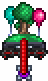
\includegraphics{images/3.png}
\qquad
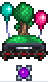
\includegraphics{images/4.png}
\end{center}
\caption{}
\label{i3:4}
\end{figure}

\subsection{传送带驱动}

传送带驱动是结构最简单、占地最小的满频驱动,其电路图见\autoref{i5:6}。在这个电路中,加重压力板是电源,传送带是用电器。要触发此驱动,只需要玩家站在传送带上。传送带使玩家向右移动,玩家进入加重压力板所在格时激活加重压力板,进而激活传送带,传送带变为逆时针,玩家向左移动,移出加重压力板时又激活加重压力板,传送带变为顺时针,玩家向右移动,如此反复。红线上的信号即为驱动信号。需要注意的是,玩家进入压力板的“瞬间”即向左移动,移出压力板的“瞬间”即向右移动,所以该驱动的频率等于电脑判断玩家与压力板是否重叠的频率,即帧率。

\begin{figure}[!ht]
\begin{center}

\includegraphics{images/5.png}
\qquad
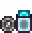
\includegraphics{images/6.png}
\end{center}
\caption{传送带驱动。图中传送带为顺时针。}
\label{i5:6}
\end{figure}

\subsection{自动门}

很多人刚开始玩泰拉瑞亚的时候,盖房子都会造门。普通的门是非常不方便的,不光出入都需要操作,门的两边不能有障碍物,而且有些时候并不能阻止敌怪进入。解救了机械师后,自然就会把普通的门改成装有制动器的物块(\autoref{i38:39}),这样的门两边可以有障碍物,而且血月也不会被开门。为了节省出入门的额外操作,就发明了自动门,它可以在玩家出入门时自动打开,出入门后自动关闭。

\begin{figure}[!ht]
\begin{center}

\includegraphics{images/38.png}
\qquad

\includegraphics{images/39.png}
\end{center}
\caption{使用制动器做的门,开关可以开关门。}
\label{i38:39}
\end{figure}

使用两个压力板就可以完成这个功能。如\autoref{i40:41}所示,当玩家从左边走向门时,会踩到门左边的压力板,压力板激活制动器,把物块虚化。当玩家通过门时,踩到门右边的压力板,压力板激活制动器,把物块实化。玩家从右边向左走同理。

\begin{figure}[!ht]
\begin{center}

\includegraphics{images/40.png}
\qquad
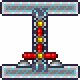
\includegraphics{images/41.png}
\end{center}
\caption{}
\label{i40:41}
\end{figure}

善于思考的人很快就会发现这个门的漏洞,那就是如果人走到门口,又回去,门就会保持开启状态。为了解决这个问题,需要把普通压力板改成加重压力板(\autoref{i44:45})。

\begin{figure}[!ht]
\begin{center}
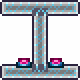
\includegraphics{images/44.png}
\qquad

\includegraphics{images/45.png}
\end{center}
\caption{}
\label{i44:45}
\end{figure}

然而改成了加重压力板后并非万事大吉。如果进入多人游戏,两个人站在门的两侧,同时试图到对方一边,那么制动器被激活两次,物块仍实化,除非一个人让步。这是非常不方便的。使用逻辑感应器(玩家)可以解决这个问题(\autoref{i46:47})。当已经有一个玩家站在感应器的蓝框内时,其他玩家进出不会改变感应器状态,感应器自然就不会激活。因此,当感应器的蓝框内有玩家时门开启,否则门关闭。

\begin{figure}[!ht]
\begin{center}
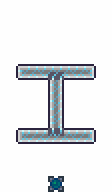
\includegraphics{images/46.png}
\qquad
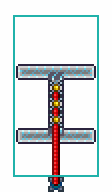
\includegraphics{images/47.png}
\end{center}
\caption{}
\label{i46:47}
\end{figure}

\subsection{刷液体机}

目前来说刷液体机主要用于会消耗液体的装置,例如2D打印机\footnote{视频链接\url{https://v.youku.com/v_show/id_XMjUwNDY5MzM4OA} 11分\\地图下载\url{http://pan.baidu.com/s/1slbFpnR}}、打开地图瞬间触发电路的模块、三液体混合反应池。另外也有人利用刷液体做一些考验电脑配置的事,比如水淹世界、水淹地狱等。

刷液体的基本原理就是泰拉瑞亚中液体的“玄学”流动机制。尽管\autoref{app23}中介绍了液体的流动机制,但是由于游戏环境下涉及到的液体格数过多,模型过于复杂,目前尚无一个完善的理论来简单预测液体的行为。一般来说,分流会导致液体增加,而在平面上摊开会导致液体减少。刷液体机大多数都是利用前景物块分流液体。由于液体的机制尚不明确,刷液体机的分流构造也都是凭经验。这里介绍刷液体机侧重点在于激活电路的方式,因此分流结构从简。

首先我们用物块搭一个有分流装置的小池子,并在底部放上入水泵,顶部放上出水泵,设置一个1秒计时器(\autoref{i7})。往池里倒上一定量的水,然后用电线连接入水泵、出水泵和1秒计时器(\autoref{i8}),右键打开1秒计时器,那么每隔一秒,入水泵上的水被传送到出水泵,刷水机就开始工作了。可以虚化一格池壁来取水。由于不同液体流速不同,刷熔岩建议使用3秒计时器,刷蜂蜜建议使用5秒计时器。

这种构造的刷液体机有一个小缺点,那就是需要手动打开计时器,因为计时器在退出地图时会自动关闭。另一方面,水充满池子的时候,水泵无效,但计时器仍在运行,这对于强迫症来说是一个打击。有一个方法可以解决这个问题,那就是在水泵边上设置液体感应器(\autoref{i9},\autoref{i10})。如果水位够高,液体感应器保持为亮,水泵不工作。如果取水使得水位下降低于液体感应器,那么液体感应器熄灭,激活水泵,水泵抽水,抽出的水经过液体感应器时点亮液体感应器,液体感应器又激活水泵,直到水位达到液体感应器时液体感应器才因保持为亮而不激活电路。这个装置不仅做到了智能刷水,而且液体感应器这个驱动频率可以完美适配液体流速。

\begin{figure}[!ht]
\begin{center}
\subfloat[]{
\label{i7}
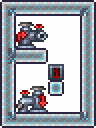
\includegraphics{images/7.png}
}
\subfloat[]{
\label{i8}
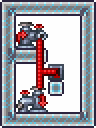
\includegraphics{images/8.png}
}
\subfloat[]{
\label{i9}
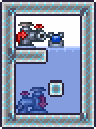
\includegraphics{images/9.png}
}
\subfloat[]{
\label{i10}
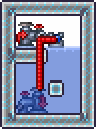
\includegraphics{images/10.png}
}
\end{center}
\caption{}
\label{i7:10}
\end{figure}

\subsection{二进制数显}

数字显示屏是一个装逼利器。事实上是,很多泰拉瑞亚视频中的数字显示屏都是整个电路中最简单的一个模块。二进制数显是最简单的一种数显。

首先用火把摆出数字“0”和“1”(\autoref{i32})。我们要让火把可以在“0”和“1”之间切换,只需要用电线连接“0”比“1”多出来的火把(\autoref{i33})。右击开关,这些火把就会在亮灭之间切换,从而数显在“0”“1”之间切换。

\begin{figure}[!ht]
\begin{center}
\subfloat[]{
\label{i32}
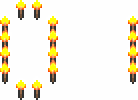
\includegraphics{images/32.png}
}
\qquad\qquad
\subfloat[]{
\label{i33}
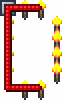
\includegraphics{images/33.png}
}
\end{center}
\caption{}
\label{i32:33}
\end{figure}

\section{逻辑门灯/逻辑门}
\begin{figure}[!ht]
\centering
\subfloat[逻辑灯]{
\includegraphics{figures/Logic_Gate_Lamp_(Off).png}\quad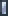
\includegraphics{figures/Logic_Gate_Lamp_(On).png}\quad
\includegraphics{figures/Logic_Gate_Lamp_(Faulty).png}}\qquad
\subfloat[逻辑门]{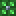
\includegraphics{figures/Logic_Gate_(AND).png}\quad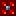
\includegraphics{figures/Logic_Gate_(NAND).png}\quad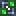
\includegraphics{figures/Logic_Gate_(OR).png}\quad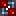
\includegraphics{figures/Logic_Gate_(NOR).png}\quad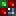
\includegraphics{figures/Logic_Gate_(XOR).png}\quad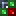
\includegraphics{figures/Logic_Gate_(XNOR).png}}
\caption{}
\end{figure}

逻辑门灯是用电器,简称为逻辑灯。逻辑灯还可以分为普通逻辑灯和故障逻辑灯。普通逻辑灯被激活时在开/关之间切换,故障逻辑灯被激活时状态被设定为“激活”(无图像效果)。逻辑灯必须堆叠在逻辑门上,我们说这些逻辑灯在该逻辑门上,该逻辑门在这些逻辑灯下。

逻辑门是电源,不同的逻辑门有不同的逻辑判定规则。如果一个逻辑门上没有故障逻辑灯,我们称其为普通逻辑门。在本节中讨论的逻辑门均为普通逻辑门。当一个逻辑门上的逻辑灯状态改变时,逻辑门会在下一个逻辑帧\footnote{逻辑帧的概念将在其有重要作用的时候详细解释,这里可以暂时认为是远小于1帧的时间。}进行逻辑判定并调整自己的亮灭状态。如果逻辑门的状态改变了,那么逻辑门会激活。

\subsection{二极管/换线器}

在开始这一小节之前,先思考一个问题:如何用一个开关同时开启多于4个的1秒计时器并使它们独立工作?

要回答这个问题,首先需要明确的一点是,如果你不确定会发生什么,用一根电线连接两个计时器是非常不靠谱的。因为计时器既是电源又是用电器,连接在一起的两个计时器在下一次激活的时候就会互相干扰,导致其中一个计时器将另一个计时器关闭。由于泰拉瑞亚中只有四种颜色的电线,如果要用一个开关同时开启多于4个计时器,那么必然有两个计时器要用同一种颜色的线激活。然而要让它们互不干扰,就意味着这两根线不能连接。同时又必须用大小只有1格的开关控制这两根线,那怎么办呢?

矛盾的根源在于,开关通过一根电线激活多个计时器后,经过一个计时器周期,计时器会通过开关上的电线互相干扰。要消除这种干扰,就要让信号既可以从开关传到计时器,又无法从计时器传到开关,即实现类似二极管的功能。

如\autoref{i13}所示,在与门上放一个逻辑灯就做成了一种二极管。用红线连接逻辑灯,蓝线连接与门(\autoref{i14},\autoref{i15}),则激活红线会导致蓝线激活,而激活蓝线不会影响红线。根据与门的定义,当逻辑灯点亮时与门点亮,当逻辑灯熄灭时与门熄灭。红线激活时,逻辑灯在亮灭之间切换,从而逻辑门也在亮灭之间切换,激活一次蓝线。由于逻辑门不是用电器,所以激活蓝线不会影响红线。

\begin{figure}[!ht]
\begin{center}
\subfloat[]{
\label{i13}
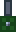
\includegraphics{images/13.png}
}
\qquad
\subfloat[]{
\label{i14}
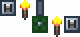
\includegraphics{images/14.png}
}
\subfloat[]{
\label{i15}
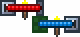
\includegraphics{images/15.png}
}
\end{center}
\caption{\ref{i14}\protect\subref{i15}:上面的开关能控制两个火把,而下面的开关只能控制一个火把}
\label{i13:15}
\end{figure}

用这个原理可以轻松用一个开关开启很多1秒计时器并使它们互不干扰(\autoref{i16:17})。

\begin{figure}[!ht]
\begin{center}
\subfloat{
\label{i16}
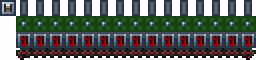
\includegraphics[width=0.4\textwidth]{images/16.png}
}
\subfloat{
\label{i17}
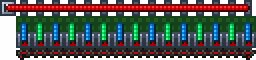
\includegraphics[width=0.4\textwidth]{images/17.png}
}
\end{center}
\caption{}
\label{i16:17}
\end{figure}

在另外一些时候,我们会用到换线器。例如我们已经预先做了一个计数器(计数器会在后面讲),它是使用蓝线输入的。同时我们做了一个驱动,该驱动使用红线输出。想用计数器来测量驱动的频率,就需要把计数器改成红线输入或者把驱动改成蓝线输出。当电路较复杂的时候,这个修改可能是非常困难的,这时就需要利用到换线器。由于这里驱动和计数器之间只是单向的信号传递,所以可以用\autoref{i13:15}中的二极管充当换线器,这样一来就解决了电线颜色不一致的问题。

\subsection{1秒延时器}

打开1秒计时器后计时器每隔1秒激活一次电路。我们希望做一个1秒延时,打开1秒延时器后,经过1秒,1秒延时器激活一次,然后关闭。

装置如\autoref{i48:49}所示。打开1秒计时器,经过1秒,计时器激活电路,然后逻辑灯被激活,进而逻辑门激活,把1秒计时器关闭。

\begin{figure}[!ht]
\begin{center}
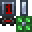
\includegraphics{images/48.png}
\qquad

\includegraphics{images/49.png}
\end{center}
\caption{}
\label{i48:49}
\end{figure}

%MappyGaming的速杀Boss方法\footnote{视频链接\url{https://www.bilibili.com/video/av13658918}}中需要精确控制召唤Boss的时间。由于秒杀拜月教邪教徒允许的误差极小,MappyGaming在召唤拜月教邪教徒时利用了电路精确控制烟花爆炸时间。电路从矿车传送到地牢开始计时,经过一段时间后触发烟花火箭杀死四个邪教徒。通过精确地控制这一段时间的长度即可以精确地控制召唤拜月教邪教徒的时间。

\subsection{改进自动门}

上一节中我们使用逻辑感应器(玩家)实现了自动门的功能。这个自动门仍有缺点,那就是感应器的感应范围太大,导致玩家在很远的地方,甚至不想开门的地方(门的上方和下方)门也会打开。加重压力板的感应范围合适,但是当门两边同时站人时会导致门关闭。我们需要实现的功能是:当门的左边站人或右边站人时门开启。因此使用或门可以达到我们的要求。

\begin{figure}[!ht]
\begin{center}
\subfloat{
\label{i50}
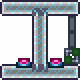
\includegraphics{images/50.png}
}
\subfloat{
\label{i51}
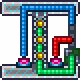
\includegraphics{images/51.png}
}
\end{center}
\caption{}
\label{i50:51}
\end{figure}

在之前的电路分析中,我们都是使用的“激活”来分析。使用激活分析总是没错的,但是在有时不如状态分析来的简单。在\autoref{i50:51}中,所有的电源与用电器都是两状态的:加重压力板有踩下和弹起两个状态,逻辑灯、逻辑门有亮灭两个状态,制动器有实化和虚化两个状态。同时,所有电源会在状态改变时激活电路,所有用电器会在电路激活时状态改变。在这种情况下,电源和用电器的状态始终是同步的,例如逻辑门亮时制动器一定是虚化状态,逻辑门灭时制动器一定是实化状态;压力板踩下时对应的逻辑灯一定亮,压力板弹起时对应的逻辑灯一定灭。我们用这种思路来分析电路:门打开=逻辑门亮=两个逻辑灯至少有1个亮=两个压力板至少有一个被踩下=门附近有人。逻辑正确。

状态分析并非万能,它只适用于电源和用电器都是两状态切换的情况下。在多数情况下仍需要用激活分析。

\subsection{绝对等价的逻辑门}
泰拉瑞亚中共有六种普通逻辑门:包括与门、与非门、或门、或非门、异或门、异或非门。

\begin{figure}[!ht]
\centering
\subfloat[]{\label{fig7}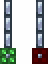
\includegraphics{images/359.png}}
\qquad
\subfloat[]{\label{fig8}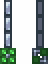
\includegraphics{images/360.png}}
\caption{}
\end{figure}

这么多种门的名字看起来十分头大,是不是必须熟悉每种门才能做电路呢?事实上,这六种门中有很多都是绝对等价的。两个装置绝对等价是指,如果把这两个装置都刷黑,那么没有任何方法可以测出它们的区别。如\autoref{fig7},左边是与门,右边是与非门,分别放上数量和状态均相同的逻辑灯后,这两个门的表现完全一致。与门和与非门的唯一区别就是,对于相同输入,与门亮时与非门一定灭,与门灭时与非门一定亮。由于逻辑门在亮灭切换时会激活,与门和与非门总是同时激活。在泰拉瑞亚中,由亮到灭的激活和由灭到亮的激活是没有区别的,所以与门和与非门没有区别。同理,或门和或非门没有区别,异或门和异或非门没有区别。

现在我们已经把需要学习的范围缩小到了三个门:与门、或门、异或门。接下来我们看\autoref{fig8},左边是与门,右边是或门,与门上全是亮灯,或门上全是灭灯。现在这两个门也是完全一致的。这是因为,它们上面的逻辑灯初始状态相反,对于相同输入,最终取值也相反。所以,与门亮$\Longleftrightarrow$与门上的所有灯亮$\Longleftrightarrow$或门上的所有灯灭$\Longleftrightarrow$或门灭。这样一来与门和或门的亮灭状态永远是相反的,类似于前面的讨论,这里的两个门也没有区别。

现在只剩下两种门了:与门、异或门。这两个有没有可能绝对等价呢?不可能,因为与门满足结合律,而异或门不满足结合律。读者在这里只需要知道,我们使用与门和异或门就足够了,其他普通逻辑门都可以用这两种门代替。

\subsection{十进制数显}\label{sec2:2}

在上一节中,我们做了一个可以显示二进制数的数显。有了逻辑门后我们就可以做十进制数显。数显视输入不同有不同的做法,这里我们使用4位二进制数输入,要求二进制数在0000\~{}1001时显示对应的十进制数0\~{}9,其他情况下显示屏熄灭。

我们选择使用七段线显示。首先用火把摆出七段线(\autoref{i34:35}\subref{i34}),然后用七根电线分别控制每一段线(\autoref{i34:35}\subref{i35})。对于0\~{}9,a\~{}g分别有对应部分点亮\autoref{qiduanxian}。

\begin{figure}[!ht]
\begin{center}
\subfloat[]{
\label{i34}
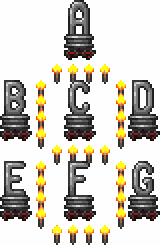
\includegraphics{images/34.png}
}
\quad
\subfloat[]{
\label{i35}
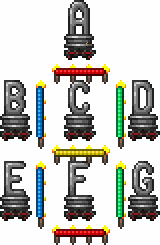
\includegraphics{images/35.png}
}
\end{center}
\caption{}
\label{i34:35}
\end{figure}

\begin{table}[!ht]
\centering
\begin{tabular}{c|c|c|c|c|c|c|c|c|c|c|c}
显示数值&0		&1	&2		&3		&4		&5		&6		&7		&8			&9\\
\hline
点亮部分&abcefg	&cf	&acdeg	&acdfg	&bcdf	&abdfg	&abdefg	&acf	&abcdefg	&abcdfg
\end{tabular}
\caption{}
\label{qiduanxian}
\end{table}

然后我们来处理输入。我们需要把输入的四位二进制信息转换为10个数字中的一个,这个过程叫做解码。我们用\autoref{i36:37}中的电路进行解码。

\begin{figure}[!ht]
\begin{center}
\subfloat[]{
\label{i36}
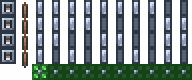
\includegraphics{images/36.png}
}
\quad
\subfloat[]{
\label{i37}
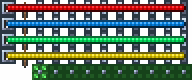
\includegraphics{images/37.png}
}
\end{center}
\caption{十个与门从左到右依次代表0\~{}9,四个开关/火把从上到下依次代表8,4,2,1。例如火把4,2,1点亮,则代表数字4+2+1=7的逻辑门点亮,其他逻辑门熄灭。}
\label{i36:37}
\end{figure}

接下来就可以进行接线了。把十个逻辑门依次标号为0\~{}9。把七段线显示器置为0状态,然后依据\autoref{qiduanxian}接线:把0号逻辑门连到abcefg,把1号逻辑门连到cf,等等。遇到电线颜色冲突的时候要使用换线器,最终连好的电路如\autoref{i42:43}。操作四个开关,显示屏即显示0\~{}9的数字或者熄灭。之所以会这样,是因为每次数字改变的时候,原有数字的逻辑门熄灭,激活一次,使原数字对应的所有火把熄灭;新数字的逻辑门点亮,激活一次,使新数字对应的所有火把点亮。

\begin{figure}[!ht]
\begin{center}
\subfloat[]{
\label{i42}
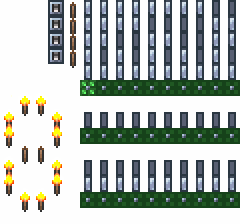
\includegraphics[width=0.3\textwidth]{images/42.png}
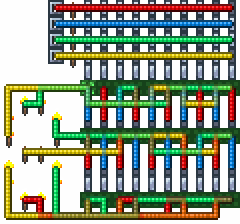
\includegraphics[width=0.3\textwidth]{images/43.png}
}
\subfloat[黄线绿线接法]{
\label{i115}
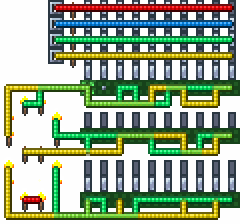
\includegraphics[width=0.3\textwidth]{images/115.png}
}
\subfloat{}
\end{center}
\caption{a连接到02356789,b连接到045689,c连接到01234789,d连接到2345689,e连接到0268,f连接到013456789,g连接到0235689。}
\label{i42:43}
\end{figure}

\section{故障逻辑门}

如果任意的普通逻辑门上有至少一个故障逻辑灯,那么该逻辑门会变为蓝色,称为故障逻辑门。故障逻辑门是一个(不是一类)特殊的逻辑门,无论其下方的普通逻辑门是什么,故障逻辑门的性质是相同的。故障逻辑门与其上最下方的故障逻辑灯之间的普通逻辑灯为有效逻辑灯。当故障逻辑门上有一个故障逻辑灯被激活时,故障逻辑门会在下一个逻辑帧依一定概率激活并把其上所有故障逻辑灯状态设定为“未激活”。该概率等于点亮的有效逻辑灯的数量除以所有有效逻辑灯的数量。请读者对照\autoref{i54:58}仔细揣摩这段话的描述。

\begin{figure}[!ht]
\begin{center}
\subfloat[]{
\label{i54}

\includegraphics{images/54.png}
}
\subfloat[]{
\label{i55}

\includegraphics{images/55.png}
}
\subfloat[]{
\label{i56}

\includegraphics{images/56.png}
}
\subfloat[]{
\label{i57}

\includegraphics{images/57.png}
}
\subfloat[]{
\label{i58}

\includegraphics{images/58.png}
}
\end{center}
\caption{当激活顶端的故障逻辑灯时,故障逻辑门激活的概率分别是:\protect\subref{i54}1/7;\protect\subref{i55}2/7;\protect\subref{i56}6/7;\protect\subref{i57}1/2;\protect\subref{i58}1。}
\label{i54:58}
\end{figure}

只有1个有效逻辑灯的故障逻辑门较特殊。因为该逻辑灯熄灭时对应的概率为0,故障逻辑门一定不激活;当逻辑灯点亮时对应概率为1,故障逻辑门一定激活。使用只有1个有效逻辑灯的故障逻辑门可以进行电路控制。

\subsection{换线器}
在普通逻辑门那里我们已经讲了换线器的做法。简单来说,换线器就是利用某些逻辑门遇输入必输出的特性。在实际应用中换线器的变种非常多。

\begin{figure}[!ht]
\centering
\subfloat[单灯换线器]{\label{fig9}\includegraphics{images/361.png}}
\qquad
\subfloat[双灯换线器]{\label{fig10}\includegraphics{images/362.png}}
\caption{换线器}
\end{figure}

单灯换线器只有一种,就是任何一个普通逻辑门上加一个逻辑灯(\autoref{fig9})。双灯换线器因为有中间的逻辑门隔开,输入和输出可以用同色的线。与门、异或门、故障门都可以做双灯换线器,如\autoref{fig10}所示。

这三种双灯换线器乍看起来又是等价的,然而实际上不是。正因为它们不等价,实际应用中可以利用它们的区别丰富我们的设计思路。

\begin{figure}[!ht]
\centering
\subfloat[与门vs故障门]{\label{fig11}\includegraphics{images/363.png}\quad\includegraphics{images/364.png}}
\qquad
\subfloat[异或门抗干扰]{\label{fig12}\includegraphics{images/365.png}\quad\includegraphics{images/366.png}}
\caption{\protect\subref{fig11}右击开关,红蓝线同时激活,左边火把不响应,右边火把响应;\protect\subref{fig12}无论蓝线如何激活,都不影响换线器工作。}
\end{figure}

首先来看与门和故障门的区别。它们的最上面的逻辑灯激活时,逻辑门都会激活。但是,如果最上面的逻辑灯同时激活两次,与门不会激活,而故障门会激活一次,对应的实验电路如\autoref{fig11}。读者可以自己实验,然后结合普通逻辑门和故障逻辑门的特性描述,思考一下为什么会这样。异或门和故障门也有同样的区别。

再来看与门和异或门的区别。与门不抗干扰,异或门抗干扰。什么意思呢?如\autoref{fig12}所示,有一根与换线器无关的电线想要横穿换线器。对于异或门,只要用图中的方法就可以避免干扰;对于与门,那么无论如何都没法避免横穿的线带来的干扰。读者可自行分析其中原因。可能你会问,有谁会自找麻烦把一根线穿过去?在实际应用中有时不得不这么做,这时异或门就提供了便利。

\subsection{置1/置0电路}\label{sec14}

泰拉瑞亚中的逻辑电路有个非常大的缺点,就是赋值困难。在数电中,想要给电路赋值0或1,只用连上对应电平的电源即可。然而在泰拉瑞亚中,电线没有电平高低,只有激活,而激活只能改变逻辑灯状态。把一个逻辑灯赋值为0,就需要在这个逻辑灯本来是1的情况下激活一次(或激活奇数次),在逻辑灯本来是0的情况下不激活(或激活偶数次)。如\autoref{i52:53}所示的电路可以做到这一点:当逻辑灯灭时,激活红线会将故障逻辑灯激活,因为逻辑灯灭,逻辑门不激活,逻辑灯保持灭。当逻辑灯亮时,激活红线会将故障逻辑灯激活,因为逻辑灯亮,逻辑门激活蓝线,逻辑灯熄灭。无论如何,激活红线都会使逻辑灯熄灭。

\begin{figure}[!ht]
\begin{center}
\subfloat{
\label{i52}
\includegraphics{images/52.png}
}
\subfloat{
\label{i53}
\includegraphics{images/53.png}
}
\end{center}
\caption{}
\label{i52:53}
\end{figure}

如果将逻辑灯与一个火把同步,就可以做到激活红线使火把熄灭。如果将逻辑灯与火把反向同步,就可以做到激活红线使火把点亮(\autoref{i59:60})。

\begin{figure}[!ht]
\begin{center}
\subfloat{
\label{i59}
\includegraphics{images/59.png}
}
\subfloat{
\label{i60}
\includegraphics{images/60.png}
}
\end{center}
\caption{左边开关使火把点亮(置1),右边开关使火把关闭(置0)。}
\label{i59:60}
\end{figure}

\subsection{D触发器}\label{sec15}

\begin{figure}[!ht]
\begin{center}
\subfloat{
\label{i237}
\includegraphics{images/237.png}
}
\qquad
\subfloat{
\label{i238}
\includegraphics{images/238.png}
}
\end{center}
\caption{左边的开关改变A火把的状态,右边的开关将A火把状态更新到B火把。}
\label{i237:238}
\end{figure}

D触发器是数电的术语,其功能非常简单,就是存储并发送状态。见\autoref{i237:238},左边的开关可以随意控制左边的火把,而右边的开关会使得右边的火把和左边的火把状态同步。换言之,D触发器存储了左边火把的值,而右边的开关命令D触发器将它存储的值发出。

回顾\nameref{sec14},它可以把火把的值设定为一个常数,而该常数可以通过故障逻辑门上的有效逻辑灯来调节。而在\autoref{}中,我们让左边的火把来调节故障逻辑门上的有效逻辑灯,当左边火把为1时,故障逻辑门变成了置1电路;当左边火把为0时,故障逻辑门变成了置0电路。这样一来,这个故障逻辑门的功能实际上是把右边火把的值置为左边火把的值。

\subsection{递次电路}

递次电路是使用频率非常高的电路。经典的递次电路如\autoref{i72:73}所示。当激活绿线时,一排故障逻辑灯被激活。但是由于只有第一个有效逻辑灯是亮的,只有第一个故障逻辑门激活,从而第一个有效逻辑灯熄灭,第二个有效逻辑灯被点亮。当再次激活绿线时,同理,第二个故障逻辑门激活,第二个有效逻辑灯熄灭,第三个有效逻辑灯点亮。依此进行,当反复激活绿线时,六个故障逻辑门依次激活并循环。将每个故障逻辑门接出一个电路,就可以实现六个电路依次运行并循环。

\begin{figure}[!ht]
\begin{center}
\subfloat{
\label{i72}
\includegraphics{images/72.png}
}
\subfloat{
\label{i73}
\includegraphics{images/73.png}
}
\end{center}
\caption{}
\label{i72:73}
\end{figure}

实际应用中的递次电路非常灵活。不仅故障逻辑门的数量可以随意变化,有效逻辑灯的亮灭、接线方式都可以视实际需求变化。递次电路的常见变种见\autoref{sec2}。使用递次电路时不要死板,要善于针对需求设计最合理的电路。

递次电路的使用非常广泛。它可以与十进制数显结合做成\url{https://www.bilibili.com/video/av22894193}中的十进制计数器,也可以做出\url{https://www.bilibili.com/video/av21009075}中的霓虹灯效果,还可以做出\url{https://www.bilibili.com/video/av6393957}中的回血回蓝大阵,等等等等等等。

递次电路的另一个典型用途就是降频。我们知道,传送带驱动的频率是60Hz。现在我们需要20Hz的驱动,只需要利用循环长度为3的递次电路(\autoref{i90:91})。

\begin{figure}[!ht]
\begin{center}
\subfloat{
\label{i90}
\includegraphics{images/90.png}
}
\subfloat{
\label{i91}
\includegraphics{images/91.png}
}
\end{center}
\caption{将黄线接出即得到20Hz的驱动,因为绿线每激活3次,黄线都激活1次。}
\label{i90:91}
\end{figure}

在一些时候,比如上面提到的十进制计数器中,我们需要“清零”操作,即将递次电路复位到初始状态。使用置0/置1电路很容易实现这一点(\autoref{i86:87})。但是这里想说明的是,对置0/置1对象的理解需要非常灵活。

\begin{figure}[!ht]
\begin{center}
\subfloat{
\label{i86}
\includegraphics{images/86.png}
}
\subfloat{
\label{i87}
\includegraphics{images/87.png}
}
\end{center}
\caption{上面的开关用来正常激活递次电路,下面的开关用来复位。除了横穿所有故障逻辑灯的绿线和黄线外,红线和蓝线用来进行递次电路中的循环并将上面有效逻辑灯的状态同步到下面,绿线和黄线用来置0/1。多加一排故障逻辑灯是为了将颜色冲突的线分开。}
\label{i86:87}
\end{figure}

是不是只有逻辑灯才有状态?在经典递次电路中,电线也可以有状态。如果我们把每根电线接到一个火把,就可以把火把的状态看作电线的状态。那么与其对逻辑灯置0/置1,不如直接对电线置0/置1,电路如\autoref{i88:89}所示。对电线进行赋值的前提是电线状态可以决定逻辑灯的状态。

\begin{figure}[!ht]
\begin{center}
\subfloat{
\label{i88}
\includegraphics{images/88.png}
}
\subfloat{
\label{i89}
\includegraphics{images/89.png}
}
\end{center}
\caption{上面的开关用来正常激活递次电路,下面的开关用来复位。}
\label{i88:89}
\end{figure}

将\autoref{i88:89}中下面一排复位电路穿插到上面递次电路的缝隙里,可以得到占用空间更小的版本(\autoref{i106:107})。

\begin{figure}[!ht]
\begin{center}
\subfloat{
\label{i106}
\includegraphics{images/106.png}
}
\subfloat{
\label{i107}
\includegraphics{images/107.png}
}
\end{center}
\caption{上面的开关用来正常激活递次电路,下面的开关用来复位。}
\label{i106:107}
\end{figure}

另外,偶尔我们可能需要用到双向递次电路,它的各种做法见\autoref{sec3}。

\subsection{降频电路}\label{sec2:1}

我们已经讲过了如何利用递次电路降频。例如\autoref{i92:97}\subref{i92:93}中,绿线激活奇数次时红线激活,偶数次时蓝线激活。事实上降频一半有更简单的方式。在\autoref{i92:97}\subref{i94:95}中,激活绿线会激活故障逻辑灯并同时点亮有效逻辑灯,此时故障逻辑门会激活,红线激活;再次激活绿线会激活故障逻辑灯并同时熄灭有效逻辑灯,此时故障逻辑门不激活。\autoref{i92:97}\subref{i94:95}也可以做到在绿线激活奇数次时红线激活,\autoref{i92:97}\subref{i96:97}也可以做到在绿线激活偶数次时蓝线激活。一般说的降频电路就指这种使用一个故障逻辑门,把频率降低一半的电路。一般不要求精确频率时,使用降频电路比递次电路更节省空间。

\begin{figure}[!ht]
\begin{center}
\subfloat[]{
\label{i92:93}
\includegraphics{images/92.png}
\includegraphics{images/93.png}
}
\qquad
\subfloat[]{
\label{i94:95}
\includegraphics{images/94.png}
\includegraphics{images/95.png}
}
\qquad
\subfloat[]{
\label{i96:97}
\includegraphics{images/96.png}
\includegraphics{images/97.png}
}
\end{center}
\caption{}
\label{i92:97}
\end{figure}

\subsection{十进制计数器}

在这一小节中我们将使用之前学过的模块来做一个四位带数显的十进制计数器。

计数器计数的对象是驱动或某个特定的信号源。信号源每激活一次,计数器的数字加1。因为是十进制,所以满十进一,这提示我们使用循环为10的递次电路作为计数模块。因为计数器要有清零功能,所以递次电路要带上复位电路。根据数字的书写习惯,右边低位,左边高位,所以采用反向的递次电路并且将逻辑门稍微错位使接线更顺。将低位的递次电路最后一个逻辑门的输出接上高一位递次电路的输入即可完成进位功能(\autoref{i108:109}),然后将最低位的递次电路输入接上驱动的输出即可以实现计数功能。

\begin{figure}[!ht]
\begin{center}
\subfloat{
\label{i108}
\includegraphics[width=0.9\textwidth]{images/108.png}
}
\\
\subfloat{
\label{i109}
\includegraphics[width=0.9\textwidth]{images/109.png}
}
\end{center}
\caption{绿线计数,黄线复位。最右边是个位,最左边是千位。}
\label{i108:109}
\end{figure}

对递次电路熟悉的人通过递次电路上的逻辑灯已经可以读出数字:递次电路上最右边的有效逻辑灯亮代表这一位是0,最左边的有效逻辑灯亮代表这一位是9。但是既然要面向不懂电路的用户,就需要把数字可视化,即加上数显。我们在之前已经做过一个十进制的数显,如果将那个数显的显示部分照搬过来,很容易发现显示的不对,这是因为两个数显的输入不同。之前做的数显,数字改变时显示器收到两个信号:第一个信号将之前的数字熄灭,第二个信号将新的数字点亮。而我们的递次电路的输出只是之前的数字。因为计数器中之前的数字可以唯一确定新的数字,所以我们可以直接让递次电路发出的信号激活从旧数字变成新数字需要激活的火把。另外,由于显示器是多个数字排列在一起,为了避免接线困难,应当先把数字上的线确定好,再往递次电路上接。如果选用\autoref{i110:112}\subref{i110}所示的火把排布,由于数字间只空了一格,之前用过的七段线接法就不能用了。所以我们采用的另一种七段线接法\autoref{i110:112}\subref{i112},注意某些线有重叠。利用\autoref{jishuqi}就可以完成接线(\autoref{i113:114})。注意到这里使用了故障逻辑门做换线器。

\begin{figure}[!ht]
\begin{center}
\subfloat[]{
\label{i110}
\includegraphics[width=0.45\textwidth]{images/110.png}
}
\subfloat[]{
\label{i112}
\includegraphics[width=0.45\textwidth]{images/112.png}
}
\end{center}
\caption{}
\label{i110:112}
\end{figure}

\begin{table}[!ht]
\centering
\begin{tabular}{c|c|c|c|c|c|c|c|c|c|c}
数字变化&0$\to$1&1$\to$2&2$\to$3&3$\to$4&4$\to$5&5$\to$6&6$\to$7&7$\to$8&8$\to$9&9$\to$0\\
\hline
激活部分&ad&abdeg&bcfg&abcd&acdf&bc&de&def&bc&bcef
\end{tabular}
\caption{}
\label{jishuqi}
\end{table}

\begin{figure}[!ht]
\begin{center}
\subfloat{
\label{i113}
\includegraphics[width=0.9\textwidth]{images/113.png}
}
\\
\subfloat{
\label{i114}
\includegraphics[width=0.9\textwidth]{images/114.png}
}
\end{center}
\caption{}
\label{i113:114}
\end{figure}

\subsection{降频技术}\label{sec18}
灵活使用递次电路和降频电路可以将已有的驱动时长增加为任意整数倍(\autoref{i223:228})。

\begin{figure}[!ht]
\begin{center}
\subfloat[]{
\label{i223:224}
\includegraphics{images/223.png}
\includegraphics{images/224.png}
}
\qquad
\subfloat[]{
\label{i225:226}
\includegraphics{images/225.png}
\includegraphics{images/226.png}
}
\qquad
\subfloat[]{
\label{i227:228}
\includegraphics{images/227.png}
\includegraphics{images/228.png}
}
\end{center}
\caption{\protect\subref{i223:224}两个降频电路连接,红线每激活4次火把响应一次;\protect\subref{i225:226}两个递次电路连接,红线每激活9次火把响应一次;\protect\subref{i227:228}降频电路与递次电路连接,红线每激活6次火把响应一次。}
\label{i223:228}
\end{figure}

使用上面的方法,当需要获得较大的质数倍(例如23倍)时间时使用递次电路体积过大,此时可以利用故障逻辑门的控制功能灵活地将多个降频的驱动结合(\autoref{i231:232})。这实质上是一个\hyperref[sec5]{多级递次}。

\begin{figure}[!ht]
\begin{center}
\subfloat{
\label{i231}
\includegraphics{images/231.png}
}
\qquad
\subfloat{
\label{i232}
\includegraphics{images/232.png}
}
\end{center}
\caption{开关每激活23次火把响应一次。上面的右边两个故障逻辑门用来控制,左边的输出接到计数为20的模块(5-递次电路与两个降频电路连接),右边的输出接到3-递次电路。开关激活时,起初左边输出,右边不输出,左边计数。当左边计数到20时上面的绿线激活,改变控制用的有效逻辑灯,改为右边输出,左边不输出,右边计数。当右边计数到3时激活火把并将控制用的有效逻辑灯改回。}
\label{i231:232}
\end{figure}

\subsection{骰子}

在前面的例子中,我们仅使用了有一个有效逻辑灯的故障逻辑门的控制功能。在这个例子中我们来使用故障逻辑门的概率功能。我们的目标是做一个电路,该电路有一个开关和六个火把。当激活开关时,六个输出有且仅有一个点亮,且每个火把点亮的概率都为1/6。

电路如\autoref{i98:99}所示。激活顶端黄线即可运行。下面很明显是递次电路,我们先分析上面部分,看看绿线会激活多少次。

\begin{figure}[!ht]
\begin{center}
\subfloat{
\label{i98}
\includegraphics{images/98.png}
}
\subfloat{
\label{i99}
\includegraphics{images/99.png}
}
\end{center}
\caption{}
\label{i98:99}
\end{figure}

当顶端黄线激活时,第一个故障逻辑门有5/6的概率激活。只有第一个故障逻辑门激活的前提下,后面的故障逻辑门才有可能激活,也就是说,有1-5/6=1/6的概率一次也不激活。在第一个故障逻辑门激活的前提下,第二个故障逻辑门有4/5的概率激活。只有第二个故障逻辑门激活的前提下,后面的故障逻辑门才有可能激活,也就是说,有5/6*(1-4/5)=1/6的概率仅第一个故障逻辑门激活,此时绿线激活一次。依此类推,可以得到绿线有5/6*4/5*(1-3/4)=1/6的概率激活两次,有5/6*4/5*3/4*(1-2/3)=1/6的概率激活三次,有5/6*4/5*3/4*2/3*(1-1/2)=1/6的概率激活四次,有5/6*4/5*3/4*2/3*1/2=1/6的概率激活五次。也就是说,顶端黄线激活时,绿线等可能地激活0\~{}5次。

绿线等可能地激活0\~{}5次,经过下面的递次电路,就会导致点亮的火把等可能地循环右移0\~{}5个。无论激活顶端黄线之前哪个火把是亮的,这都意味着六个火把有等可能的概率点亮。

\begin{problemset}[思考题]
\item 为什么只能由玩家激活的压力板会选用灰/棕/蓝/丛林蜥蜴这四种颜色?
\item 解释为什么如\autoref{i11:12}所示装置会在世界开启瞬间激活广播盒。该装置里的故障逻辑门有什么作用?
\begin{figure}[!ht]
\begin{center}
\subfloat{
\label{i11}
\includegraphics[width=0.4\textwidth]{images/11.png}
}
\subfloat{
\label{i12}
\includegraphics[width=0.4\textwidth]{images/12.png}
}
\end{center}
\caption{}
\label{i11:12}
\end{figure}
\item 制作一个装置,在每天入昼时显示讯息“日食正在发生...”,入夜时显示“血月正在升起...”。
\item 找出\url{https://www.bilibili.com/video/av5271577}中的延时装置。
\item 做一个显示当前月相的显示器,显示效果如\autoref{i61:68}。
\begin{figure}[!ht]
\begin{center}
\subfloat[满月]{
\label{i61}
\includegraphics[width=0.11\textwidth]{images/61.png}
}
\subfloat[亏凸月]{
\label{i62}
\includegraphics[width=0.11\textwidth]{images/62.png}
}
\subfloat[下弦月]{
\label{i63}
\includegraphics[width=0.11\textwidth]{images/63.png}
}
\subfloat[残月]{
\label{i64}
\includegraphics[width=0.11\textwidth]{images/64.png}
}
\subfloat[新月]{
\label{i65}
\includegraphics[width=0.11\textwidth]{images/65.png}
}
\subfloat[峨眉月]{
\label{i66}
\includegraphics[width=0.11\textwidth]{images/66.png}
}
\subfloat[上弦月]{
\label{i67}
\includegraphics[width=0.11\textwidth]{images/67.png}
}
\subfloat[盈凸月]{
\label{i68}
\includegraphics[width=0.11\textwidth]{images/68.png}
}
\end{center}
\caption{}
\label{i61:68}
\end{figure}
\item 实现\url{https://www.bilibili.com/video/av5271577} 2分57秒处神庙尖刺的效果。
\item 设计如\autoref{i69:70}所示的二进制数显。
\begin{figure}[!ht]
\begin{center}
\subfloat[0]{
\label{i69}
\includegraphics{images/69.png}
}
\qquad
\subfloat[1]{
\label{i70}
\includegraphics{images/70.png}
}
\end{center}
\caption{}
\label{i69:70}
\end{figure}
\item 补全十进制数显\autoref{i71}的接线。
\begin{figure}[!ht]
\centering
\includegraphics{images/71.png}
\caption{}
\label{i71}
\end{figure}
\item 为什么十进制带数显的计数器一般不会多于四位?
\item 利用降频电路和二进制数显制作一个多位的二进制计数器。
\item 做一个可以显示点数的骰子,六个点数效果如\autoref{i100:105}。
\begin{figure}[!ht]
\begin{center}
\subfloat[1]{
\label{i100}
\includegraphics[width=0.15\textwidth]{images/100.png}
}
\subfloat[2]{
\label{i101}
\includegraphics[width=0.15\textwidth]{images/101.png}
}
\subfloat[3]{
\label{i102}
\includegraphics[width=0.15\textwidth]{images/102.png}
}
\subfloat[4]{
\label{i103}
\includegraphics[width=0.15\textwidth]{images/103.png}
}
\subfloat[5]{
\label{i104}
\includegraphics[width=0.15\textwidth]{images/104.png}
}
\subfloat[6]{
\label{i105}
\includegraphics[width=0.15\textwidth]{images/105.png}
}
\end{center}
\caption{}
\label{i100:105}
\end{figure}
\end{problemset}
\chapter{逻辑结算}\label{sec7}

在上一章中我们介绍了很多电路模块。这时候读者如果想当然地把这些电路模块组合起来,容易发生一些意想不到的问题,这也是上一章没有介绍过多复合电路的原因。在这一章中,我们将完善整个逻辑结算中的所有细节,确保可以预测任何复合逻辑电路的行为。

在一个逻辑电路中,每个电源和用电器可以接多根线,每根线可以接多个电源和用电器。当电路激活时,所有电源、电线、用电器都会按照一定顺序激活。

非常明显的结论是,电源激活后,电源上的电线激活,然后电线下的用电器激活。进一步的,如果电源$A$比电源$B$先激活,那么电源$A$上的电线也应当比$B$上的电线先激活;如果电线$a$比电线$b$先激活,那么$a$下的所有用电器也应当比$b$下的所有用电器先激活;如果逻辑门$A$上的逻辑灯比逻辑门$B$上的逻辑灯先激活,那么逻辑门$A$也应当比逻辑门$B$先激活。

以上的一些规则都是合理的,很容易理解。接下来的规则则是泰拉瑞亚特有的,需要进行记忆。

当一个电源激活后,其上的四色电线,按照红、蓝、绿、黄的先后顺序激活。

当一根电线激活后,其上各点按照距离电源由近到远的顺序激活。到电源距离相等的点,理解激活顺序需要理解图的广度优先搜索(BFS)算法,这里不详细解释。

对于涉及到逻辑门的电路,电路结算被分步进行。每一步中都进行逻辑门激活——电线激活——逻辑灯激活——逻辑门判断这四小步。逻辑灯被激活后,暂时不进行逻辑判断,等到所有电线结算完毕后,再统一进行逻辑判断。这每一步叫做\textbf{逻辑帧}。一个逻辑电路的结算过程中,反复运行每个逻辑帧中的四小步,直到没有逻辑门需要激活。

除了逻辑门以外的电源叫做\textbf{物理电源}。一个逻辑结算必须通过物理电源的激活启动。一个逻辑结算中一个逻辑门只能激活至多一次。如果它尝试激活第二次,那么激活失败并有白烟从逻辑门发出,称为\textbf{爆门}。逻辑门状态仍然会正常切换但是不会发出信号。爆门属于正常机制,是开发者有意为之,加以利用也可以起到作用。

\section{用 MechScope 模组研究电路结算过程}
MechScope 模组可以将电路结算过程可视化。其下载链接已经在\autoref{sec1:1}中给出。安装该模组后,在游戏内可以看到电路的结算过程。

\begin{figure}[!h]
\includegraphics[width=0.95\textwidth]{images/273.png}
\caption{MechScope模组}\label{i273}
\end{figure}

进入游戏后,打开设置——控制,可以看到MechScope的键位设置。默认键位为:
\begin{itemize}
\item[小键盘1] Toggle(触发)
\item[小键盘2] Step(步进)
\item[小键盘3] Auto Step(自动步进)
\item[小键盘5] Settings(设置)
\end{itemize}

如\autoref{i274}所示,先做一个最简单的电路。在这个电路中,开关通过一根红线控制火把。
\begin{figure}[!h]
\begin{center}
\subfloat[]{\label{i274}\includegraphics{images/274.png}}
\qquad
\subfloat[]{\label{i277}\includegraphics{images/277.png}}
\end{center}
\caption{}
\end{figure}

按下小键盘1,可以看到光标右上角有一个黄点(\autoref{i275}),表示MechScope正在运行。
\begin{figure}[!h]
\begin{center}
\subfloat[]{\label{i275}\includegraphics{images/275.png}}
\qquad
\subfloat[]{\label{i276}\includegraphics{images/276.png}}
\end{center}
\caption{}
\end{figure}

右键点击开关,此时电路会被暂停。开关上显示一个红框,电线所在格加了一层红色滤镜,分别表示激活的电源和电线(\autoref{i277})。火把已经熄灭。光标右上角的黄点变成了红点(\autoref{i276}),表示有正在运行的电路。按一下小键盘2进行步进,电路结算完成,光标右上角恢复黄点。

了解了基本操作,我们来看设置菜单。按下小键盘5,打开设置菜单(\autoref{i278})。前四项是单选,表示每次步进的幅度。Single是逐格步进,Wire是逐线步进,Source是逐源步进,Stage是逐逻辑帧步进。后六项是显示设置,仅影响可视化程度,这里不进行介绍,读者可自行尝试。最后一个数字是自动步进的周期/物理帧,这个值越小,自动步进越快。
\begin{figure}
\centering
\includegraphics[width=0.3\textwidth]{images/278.png}
\caption{MechScope的设置菜单}\label{i278}
\end{figure}

我们的重心放在前四项设置,它们是有关于电路结算的,其中Stage是关于逻辑结算的。

\subsection{逐格步进}
设置菜单中选择逐格步进,然后做出\autoref{i274_2}所示的电路。打开MechScope,右键点击开关,可以看到开关上出现了红框,表示开关作为电源,激活了它上面的红线(\autoref{i279})。按下小键盘2步进,开关右边一格出现了红框,表示这一格激活(\autoref{i280})。反复步进,红框一直向右移动直到火把上,把火把关闭。
\begin{figure}
\begin{center}
\subfloat[]{\label{i274_2}\includegraphics[width=0.27\textwidth]{images/274.png}}\\
\subfloat[]{\label{i279}\includegraphics[width=0.27\textwidth]{images/279.png}}
\qquad
\subfloat[]{\label{i280}\includegraphics[width=0.27\textwidth]{images/280.png}}
\qquad
\subfloat[]{\label{i281}\includegraphics[width=0.27\textwidth]{images/281.png}}
\qquad
\subfloat[]{\label{i282}\includegraphics[width=0.27\textwidth]{images/282.png}}
\qquad
\subfloat[]{\label{i283}\includegraphics[width=0.27\textwidth]{images/283.png}}
\qquad
\subfloat[]{\label{i284}\includegraphics[width=0.27\textwidth]{images/284.png}}
\end{center}
\caption{}
\end{figure}

这个实验展示了单根电线上的激活顺序:电线由近到远依次激活。不过它只展示了单向传播的情况。对于复杂的情况,读者可以自己使用MechScope模组研究。一般情况下我们只需要知道距离电源近的先激活,距离电源远的后激活,这里的距离指沿电线到电源最短路径的长度。这里为计算机专业的同学提供一个信息:单根电线是按照从电源开始广度优先搜索的顺序激活的,四个方向的顺序是下上右左。

\subsection{逐线步进}
设置菜单中选择逐线步进,然后做出\autoref{i285}所示的电路。在逐线步进模式下,每次步进会前进一整根电线。右键点击开关,可以看到红线激活(\autoref{i286});步进,蓝线激活(\autoref{i287});步进,绿线激活(\autoref{i288});步进,黄线激活(\autoref{i289})。
\begin{figure}
\begin{center}
\subfloat[]{\label{i285}\includegraphics[width=0.27\textwidth]{images/285.png}}
\qquad
\subfloat[]{\label{i286}\includegraphics[width=0.27\textwidth]{images/286.png}}
\qquad
\subfloat[]{\label{i287}\includegraphics[width=0.27\textwidth]{images/287.png}}
\qquad
\subfloat[]{\label{i288}\includegraphics[width=0.27\textwidth]{images/288.png}}
\qquad
\subfloat[]{\label{i289}\includegraphics[width=0.27\textwidth]{images/289.png}}
\end{center}
\caption{}
\end{figure}

这个实验展示了单个电源上不同电线的激活顺序:红线、蓝线、绿线、黄线依次激活。

\subsection{逐逻辑帧步进}
我们先跳过逐源步进,来看逐逻辑帧步进。电路如\autoref{i290}所示。在逐逻辑帧步进模式下,每次步进会前进一个逻辑帧。
\begin{figure}
\begin{center}
\subfloat[]{\label{i290}\includegraphics[width=0.27\textwidth]{images/290.png}}\\
\subfloat[]{\label{i291}\includegraphics[width=0.27\textwidth]{images/291.png}}
\qquad
\subfloat[]{\label{i292}\includegraphics[width=0.27\textwidth]{images/292.png}}
\qquad
\subfloat[]{\label{i293}\includegraphics[width=0.27\textwidth]{images/293.png}}
\qquad
\subfloat[]{\label{i294}\includegraphics[width=0.27\textwidth]{images/294.png}}
\qquad
\subfloat[]{\label{i295}\includegraphics[width=0.27\textwidth]{images/295.png}}
\qquad
\subfloat[]{\label{i296}\includegraphics[width=0.27\textwidth]{images/296.png}}
\end{center}
\caption{}\label{i290:296}
\end{figure}

我们一般把\textbf{物理电源}\footnote{物理电源是除逻辑门以外的电源。}激活时的逻辑帧记作第0个逻辑帧(\autoref{i291}),往后每个逻辑帧都进行逻辑门激活,电线激活,逻辑灯激活,逻辑门判断。在\autoref{i290:296}中,从\subref{i291}到\subref{i296}分别是第0个逻辑帧到第5个逻辑帧,每个逻辑帧中都用加粗方框标出了激活的逻辑门,滤镜标出了激活的电线,“×”标出了已经激活过的逻辑门,“○”标出了在下一逻辑帧将要激活的逻辑门。

\begin{figure}
\begin{center}
\subfloat[]{\label{i297}\includegraphics[width=0.45\textwidth]{images/297.png}}\\
\subfloat[]{\label{i298}\includegraphics[width=0.45\textwidth]{images/298.png}}
\qquad
\subfloat[]{\label{i299}\includegraphics[width=0.45\textwidth]{images/299.png}}
\qquad
\subfloat[]{\label{i300}\includegraphics[width=0.45\textwidth]{images/300.png}}
\qquad
\subfloat[]{\label{i301}\includegraphics[width=0.45\textwidth]{images/301.png}}
\end{center}
\caption{}\label{i297:301}
\end{figure}

再来看一个稍复杂的电路(\autoref{i297})。右键点击开关,进入第0个逻辑帧(\autoref{i298}):开关作为电源激活,开关上的红线激活,两个逻辑灯激活,两个逻辑门进行判断,并计划激活(逻辑门上画了一个小的红圈)。

第1个逻辑帧(\autoref{i299})。两个逻辑门作为电源激活,蓝线和绿线激活,三个逻辑灯及火把激活。其中火把改变状态,左右两个逻辑灯改变状态,中间的逻辑灯因为激活了两次,状态不变。三个逻辑灯下的逻辑门进行判断,其中左右两个逻辑门计划激活,中间的逻辑门不计划激活。

第2个逻辑帧(\autoref{i300})。两个逻辑门作为电源激活,两根红线激活,四个逻辑灯及火把激活,全部改变状态。四个逻辑门计划激活。

第4个逻辑帧(\autoref{i301})。四个逻辑门作为电源激活,蓝线激活四次,火把激活四次,状态不变。没有计划激活的逻辑门,逻辑结算结束。

\subsection{爆门}

来看\autoref{i302},这是一个循环电路,看起来,红线在第0个逻辑帧激活,蓝线在第1个逻辑帧激活,红线又在第2个逻辑帧激活,蓝线又在第三个逻辑帧激活……如果真是这样,那么游戏会崩溃,因为泰拉瑞亚中,无论电路有多复杂,都必须要在一个物理帧内结算完毕。如果1/60秒没法结算完的话,物理帧会相应的加长,导致帧率降低。如果永远结算不完,那么游戏就会卡在一个物理帧中,无法进行任何操作。

泰拉瑞亚使用了一种傻瓜方法来规避这种死循环。一个逻辑门激活后,会有一个标记,在MechScope中会显示一个白色的“×”。如果之后这个逻辑门还计划激活(MechScope显示红色的“○”),那么取消这个计划,并且播放爆门动画(冒烟)。在\autoref{i302:305}中,爆门的行为发生在\autoref{i305},即上面的逻辑门再次计划激活时。截图没能截下爆门的瞬间,读者可以自行尝试。

\begin{figure}
\begin{center}
\subfloat[]{\label{i302}\includegraphics[width=0.1\textwidth]{images/302.png}}
\qquad
\subfloat[]{\label{i303}\includegraphics[width=0.1\textwidth]{images/303.png}}
\qquad
\subfloat[]{\label{i304}\includegraphics[width=0.1\textwidth]{images/304.png}}
\qquad
\subfloat[]{\label{i305}\includegraphics[width=0.1\textwidth]{images/305.png}}
\end{center}
\caption{}\label{i302:305}
\end{figure}

之所以称之为“傻瓜方法”,是因为它有副产物。换句话讲,对于不会死循环的电路也会发生爆门。在\autoref{i306:308}中,下方的逻辑门在第1个逻辑帧激活,并被标记了“×”。第1个逻辑帧中,蓝线激活,下方的逻辑灯状态改变,所以逻辑门又要计划激活,结果爆门。

\begin{figure}
\begin{center}
\subfloat[]{\label{i306}\includegraphics[width=0.1\textwidth]{images/306.png}}
\qquad
\subfloat[]{\label{i307}\includegraphics[width=0.1\textwidth]{images/307.png}}
\qquad
\subfloat[]{\label{i308}\includegraphics[width=0.1\textwidth]{images/308.png}}
\end{center}
\caption{}\label{i306:308}
\end{figure}

从上面两个例子中我们总结一下爆门的原因。一个逻辑门在一次电路结算中至多只会激活一次。如果尝试再次激活,那么激活失败并爆门。需要注意的是,逻辑门状态仍会照常改变。

在实际应用中,爆门经常导致电路bug,这是因为我们往往希望逻辑门在多次状态切换时可以多次激活,但实际上不会。学会了预测爆门,就可以想办法避免爆门,甚至利用爆门。

%\section{使用逻辑延迟器规避爆门}

%我们已经知道了,降频电路可以用来做二进制计数。我们还知道,


\section{逻辑延迟器}

在连接多个逻辑电路模块时,要让它们正确地合作,就需要控制它们的运行顺序。不同电路模块从输入到输出经历的逻辑帧数量不同,所以简单的接线方式可能使得一些模块在不该工作时工作,打乱电路状态。使用逻辑延迟器可以推迟一个电路模块的运行逻辑帧,使得这个电路模块在需要运行的时候才运行。

上一章讲到的换线器就可以作为逻辑延迟器,因为输出激活比输入激活晚一个逻辑帧。如果将多个换线器首尾连接,就可以控制延迟的逻辑帧数量。

\begin{figure}[!h]
\begin{center}
\subfloat[横式]{
\label{i153}
\includegraphics{images/153.png}
}
\qquad
\subfloat[竖式]{
\label{i154}
\quad\includegraphics{images/154.png}\quad
}
\qquad
\subfloat[斜式]{
\label{i155}
\includegraphics{images/155.png}
}
\qquad
\subfloat[双竖式]{
\label{i156}
\quad\includegraphics{images/156.png}\quad
}
\end{center}
\caption{逻辑延迟器的不同摆法,逻辑延迟均为3个逻辑帧。}
\label{i153:156}
\end{figure}

\section{普通逻辑门的逻辑同步}
对于有数电基础的玩家,刚涉及泰拉瑞亚电路时会遇到各种各样的爆门。而通过各种各样教学视频入门的“外行”反而不容易遇到这样的问题。

爆门的原因是一个逻辑门在一次逻辑结算中激活多次。虽然故障逻辑门也可以发生爆门(下一节会讲),但是普通逻辑门才是爆门的重灾区。我们在使用普通逻辑门的时候,一般都是要进行简单的组合逻辑运算,比如几个与逻辑,几个异或逻辑的结合。这样的逻辑运算当然是可以进行状态判断的而不需要使用激活判断。可以进行状态判断的前提是,一根线连接的所有电源和用电器的状态要同步,换句话就是,电源状态改变时,和电源连接的所有用电器状态也要改变。但是当爆门发生时,逻辑门状态改变却不发出信号,这样就会导致用电器状态不变,电路就无法进行状态判断了。不能进行状态判断的电路就没办法做组合逻辑。

举一个简单的例子。我们知道降频电路(\autoref{sec2:1})可以做二进制计数,而\autoref{sec2:2}中的电路可以将二进制编码转成十进制显示。那么自然而然就会想到,把这两个电路连起来不就可以进行十进制计数了吗?

这里仅给出精简版的电路来说明这样做不对。如\autoref{},仅用一个降频电路,那么可以计四个数,用四个双灯与门进行解码,输出到四个火把。

开关第一次激活,仅红线激活,激活后各逻辑灯与逻辑门的状态如\autoref{},所以第一个门和第二个门激活,第一个火把熄灭,第二个火把点亮。开关第二次激活,红线与蓝线都激活,但是红线比蓝线早一个逻辑帧。红线激活后各逻辑灯与逻辑门状态如\autoref{},此时第一个门和第二个门激活,第一个火把点亮,第二个火把熄灭。蓝线激活后各逻辑灯与逻辑门状态如\autoref{},此时第一个门和第三个门激活,但是第一个门已经激活过了,所以爆门,只有第三个门激活,所以第三个火把点亮。到这里可以看出来,尽管逻辑门的状态是对的,即只有第三个逻辑门是亮的,但是火把状态不对,这是因为第一个门爆门后第一个火把少了一次激活。

导致这个爆门的原因是红线比蓝线早一个逻辑帧,解决起来也很简单,那就是在红线上做一个逻辑延迟,让红线和蓝线在同一个逻辑帧激活。

\section{爆门}

当一个逻辑门在逻辑结算中尝试激活多次时就会引起爆门。引起爆门的方式有多种(\autoref{i150:152})。

\begin{figure}[!h]
\begin{center}
\subfloat[]{
\label{i150}
\includegraphics[width=0.32\textwidth]{images/150.png}
}
\subfloat[]{
\label{i151}
\includegraphics[width=0.32\textwidth]{images/151.png}
}
\subfloat[]{
\label{i152}
\includegraphics[width=0.32\textwidth]{images/152.png}
}
\end{center}
\caption{可能引起爆门的三种原因。\protect\subref{i150}一个普通逻辑门的不同逻辑灯在不同逻辑帧激活;\protect\subref{i151}一个普通逻辑门的一个逻辑灯在多个不同逻辑帧激活;\protect\subref{i152}一个故障逻辑灯在多个不同逻辑帧激活。}
\label{i150:152}
\end{figure}

爆门只是一个机制,并非bug,所以它也有可以应用的价值。例如,使用爆门可以将横式的逻辑延迟器体积大大缩小(\autoref{i157})。

\begin{figure}[!h]
\centering
\includegraphics{images/157.png}
\caption{改进的横式逻辑延迟器}
\label{i157}
\end{figure}

\section{状态表示与激活表示}

泰拉瑞亚电路中的信号有两种表示方式:状态表示和激活表示。状态表示一般是显式的,即肉眼可以直接通过电路元件的状态读出其要表示的信息,例如亮表示1,灭表示0。激活表示是隐式的,激活表示1,不激活表示0。因为激活对于任何有显示效果的物品(像素盒除外)都只能改变其状态,因此想读出激活的信息,就需要在电路元件激活前和激活后的状态之间比较,状态变化的是1,状态不变的是0。这种读法显然是不方便的。

从电路运行角度,状态表示与激活表示经常需要搭配使用。普通逻辑门一般适用于状态表示,而故障逻辑门适用于激活表示。无论是为了产生可读性输出,还是为了在各电路模块之间传输信息,都会用到在状态表示与激活表示之间互换的方法。这一节中就将介绍将状态表示与激活表示互换的方法。

\subsection{状态表示转为激活表示}

一个故障逻辑门就可以做到将亮转变为激活,灭转变为不激活的功能。需要注意的是,仅用一个故障逻辑门的话,即使有效逻辑灯在一个逻辑结算中多次在亮灭之间切换,逻辑门也至多只能激活一次。所以更细分,有点亮立刻激活(\autoref{i173:175}\subref{i174})与事后激活(\autoref{i173:175}\subref{i175})两种造法。

\begin{figure}[!h]
\begin{center}
\subfloat[]{
\label{i173}
\includegraphics{images/173.png}
}
\qquad
\subfloat[]{
\label{i174}
\includegraphics{images/174.png}
}
\qquad
\subfloat[]{
\label{i175}
\includegraphics{images/175.png}
}
\end{center}
\caption{红线控制有效逻辑灯状态。\protect\subref{i174}有效逻辑灯点亮时立刻激活;\protect\subref{i175}事后激活,在某个时刻激活蓝线可以将有效逻辑灯的亮/灭转换为故障逻辑门的激活/不激活。}
\label{i173:175}
\end{figure}

点亮瞬间激活使用的就是降频电路,这里不作详细解释。事后激活即在某个时候(逻辑帧)中对于状态为1的激活,状态为0的不激活。

\subsection{激活表示转为状态表示}

激活转状态,需要将激活转变为点亮,不激活转变为熄灭。电路设计时需要特别注意“不激活”时的响应,因为按照电路原理,不激活时是不会有用电器响应的。如果要响应“不激活”,就必须在某个时间令电路执行不激活时的响应,即事前置0(\autoref{i173:176})或事后置0。

\begin{figure}[!h]
\begin{center}
\subfloat[]{
\label{i173b}
\includegraphics{images/173.png}
}
\qquad
\subfloat[]{
\label{i176}
\includegraphics{images/176.png}
}
\end{center}
\caption{无论红线是否激活,首先激活蓝线将有效逻辑灯置0,随后红线激活则有效逻辑灯变为1,否则有效逻辑灯为0。}
\label{i173:176}
\end{figure}

事前置0使用置0电路,在电路运行时先将火把置0,然后若输入激活,则火把变为1,否则火把保持为0,就完成了激活转状态的功能。

事后置0既要使用置0电路也要使用置1电路。首先输入激活则激活置1电路,火把变为1,然后当电路运行结束时激活置0电路将所有其他火把置为0。要让置0电路不影响刚激活了的火把,需要使用额外的逻辑门记录本次逻辑结算中的激活状态,本质上还需要使用事前电路,因此这里不详细讨论。

\subsection{事前电路与事后电路}

事前电路,即在某个电路模块运行之前执行的电路;事后电路,即在某个电路模块运行之后执行的电路。把事前和事后的概念放在这一章,是因为控制它们执行的时机需要逻辑帧知识,并且有时需要在电路中添加逻辑延迟器来控制运行的时机。

从之前的讨论可以看出,状态转激活用事后电路较好,激活转状态用事前电路较好。

\subsection{可以随机显示的十进制数显}

上一章我们做的十进制数显输入还不够自由:要么需要输入二进制,要么需要连续数字。一个完美意义下的十进制数显应该接收11个输入,前十个输入激活则显示0\~{}9的数字,最后一个输入激活则全部熄灭。

显示0\~{}9的数字对应的是火把状态,而输入是激活。因此需要一个将激活转化为状态的电路。如\autoref{i127:128},在火把上加上事前置0电路。无论激活哪个开关,事前置0电路都会在第0个逻辑帧激活,在第1个逻辑帧生效。显示电路在第0个逻辑帧激活,在第1至2个逻辑帧生效。

\begin{figure}[!h]
\begin{center}
\subfloat{
\label{i127}
\includegraphics[width=0.45\textwidth]{images/127.png}
}
\qquad
\subfloat{
\label{i128}
\includegraphics[width=0.45\textwidth]{images/128.png}
}
\end{center}
\caption{}
\label{i127:128}
\end{figure}

\section{密码门}

\section{随机分两组}

上一章我们学习了骰子的电路,即从n个元素里随机选取出1个。这一节中将介绍从n个元素里随机选取m个(或将n个元素随机分成两组,每组的元素数量分别为m和n-m)的电路。要理解本节内容需要有高中的概率知识。我们以随机8选4为例。

首先考虑需要用到哪些概率的故障逻辑门。
\begin{itemize}
\item 第一个元素有4/8的概率分到第1组。
\item 第一个元素的分组确定后就可以来给第二个元素分组,这时有两种情况。如果第一个元素分到了第1组,那么第二个元素有3/7的概率分到第1组,否则该概率为4/7。
\item 同理,如果前两个元素全部分到了第1组,那么第三个元素有2/6的概率分到第1组;如果前两个元素中只有1个分到了第1组,那么第三个元素有3/6的概率分到第1组;如果前两个元素全部分到了第2组,那么第三个元素有4/6的概率分到第1组。
\item 如果前三个元素有3/2/1/0个分到了第1组,那么第四个元素有$\frac{1}{5}/\frac{2}{5}/\frac{3}{5}/\frac{4}{5}$的概率分到第1组。
\item 如果前四个元素有4/3/2/1/0个分到了第1组,那么第五个元素有$\frac{0}{4}/\frac{1}{4}/\frac{2}{4}/\frac{3}{4}/\frac{4}{4}$的概率分到第1组。
\item 如果前五个元素有4/3/2/1个分到了第1组,那么第六个元素有$\frac{0}{3}/\frac{1}{3}/\frac{2}{3}/\frac{3}{3}$的概率分到第1组。
\item 如果前六个元素有4/3/2个分到了第1组,那么第七个元素有$\frac{0}{2}/\frac{1}{2}/\frac{2}{2}$的概率分到第1组。
\item 如果前七个元素有4/3个分到了第1组,那么第八个元素有$\frac{0}{1}/\frac{1}{1}$的概率分到第1组。
\end{itemize}

乍一看这就需要24个故障逻辑门,还没有算上控制电路。如果m和n再稍微大点,就是天文数字了。仔细观察可以发现,每个元素的分组概率虽然有很多个可能值,但是这些概率都有两个特点:分母相同;分子与之前元素的分组情况有非常简单的关系。这就提醒我们使用之前元素的分组状态直接修改后续故障逻辑门的有效逻辑灯的亮灭,从而修改后续元素的分组概率。

用于概率的故障逻辑门组如\autoref{i126}所示。

\begin{figure}
\centering
\includegraphics{images/126.png}
\caption{}
\label{i126}
\end{figure}

激活第一个故障逻辑灯,第一个故障逻辑门有4/8概率激活。我们假设逻辑门激活代表对应元素被分到第1组。当第一个故障逻辑门未激活时,我们希望第二个故障逻辑门保持当前的4/7的概率;当第一个故障逻辑门激活时,我们希望第二个故障逻辑门的概率被修改为3/7,即有一个点亮的有效逻辑灯被熄灭。总而言之,只要第1组和第2组都没有排满,之前的逻辑门每激活一次,都会使后面逻辑门的概率降低。当第1组或第2组已经分到4个元素时,后面逻辑门的概率都保持在0或1不变了。

由于后面逻辑门的概率降低是根据之前逻辑门激活的次数确定的,所以使用递次电路完成这个计数功能。递次电路以所有用于概率的故障逻辑门作为输入。递次电路激活1次,表示有一个元素分到了第1组,将从下到上第4排有效逻辑灯熄灭,使后面分组的分子至多为3;递次电路激活2次,表示有两个元素分到了第1组,再将从下到上第3排有效逻辑灯熄灭,使后面分组的分子至多为2;...;递次电路激活4次,表示已经有4个元素分到了第1组,将最下面一排有效逻辑灯熄灭,此时所有有效逻辑灯熄灭,代表后面的概率全部为0,即剩余所有元素都被分到第2组。为接线方便,采用斜向的递次电路(\autoref{i130:131})。

\begin{figure}[!h]
\begin{center}
\subfloat{
\label{i130}
\includegraphics[width=0.45\textwidth]{images/130.png}
}
\qquad
\subfloat{
\label{i131}
\includegraphics[width=0.45\textwidth]{images/131.png}
}
\end{center}
\caption{}
\label{i130:131}
\end{figure}

为重复使用,复位电路也是必须的,即将八个用于概率的故障逻辑灯全部激活后将电路恢复到初始状态。全部激活后,递次电路一定被激活了4次,所以递次电路已经自动复位;有效逻辑灯一定全灭,复位电路只需要将需要的有效逻辑灯全部点亮即可(\autoref{i132:133})。

\begin{figure}[!h]
\begin{center}
\subfloat{
\label{i132}
\includegraphics[width=0.45\textwidth]{images/132.png}
}
\qquad
\subfloat{
\label{i133}
\includegraphics[width=0.45\textwidth]{images/133.png}
}
\end{center}
\caption{}
\label{i132:133}
\end{figure}

在上面的电路中,我们需要依次从左到右点击八个开关,对应的故障逻辑门激活代表对应的元素被分到第1组\footnote{注意这里用激活表示分组,因此如果使用火把显示,需要额外的置0电路。}。分完以后需要点击第九个开关复位。理想的电路当然是希望只需要点一次开关就自动完成所有功能。整个电路的运行顺序应该是:第一个故障逻辑灯激活,第一个故障逻辑门(可能)激活后,递次电路激活,修改有效逻辑灯,然后第二个故障逻辑灯激活,……八个故障逻辑灯激活后,复位电路激活。因此每两个相邻的故障逻辑灯之间需要有逻辑延迟,最后一个故障逻辑灯和复位电路之间有逻辑延迟。接下来需要计算至少需要延迟几个逻辑帧。

当一个用于概率的故障逻辑灯在第k个逻辑帧激活后,该故障逻辑门在第k+1个逻辑帧激活,并激活递次电路;递次电路在第k+2个逻辑帧激活,并将对应的有效逻辑灯关闭。因此下一个故障逻辑灯激活时机不能早于第k+2个逻辑帧,否则概率还没有修改。也就是说,相邻两个故障逻辑灯之间的逻辑延迟至少为2个逻辑帧。

当最后一个用于概率的故障逻辑灯在第k个逻辑帧激活后,该故障逻辑门在第k+1个逻辑帧激活,并激活递次电路;递次电路在第k+2个逻辑帧激活并关闭对应的有效逻辑灯。由于递次电路和复位电路都只是对有效逻辑灯做操作,因此谁先谁后对电路运行结果没有影响,只需要复位电路运行时不干扰到故障逻辑门的概率判断即可。因此复位电路激活时机不早于第k+1个逻辑帧,即复位电路至少比最后一个故障逻辑灯晚一个逻辑帧激活。

捋好这些逻辑后就可以接线了。如\autoref{i134:135},在每两个相邻的故障逻辑灯之间加两个换线器用来构造2个逻辑帧的延迟;在最后一个故障逻辑灯和复位电路之间加一个换线器用来构造1个逻辑帧的延迟。火把上加了事前置0电路用来将激活转换为点亮。

\begin{figure}[!h]
\begin{center}
\subfloat{
\label{i134}
\includegraphics[width=0.45\textwidth]{images/134.png}
}
\qquad
\subfloat{
\label{i135}
\includegraphics[width=0.45\textwidth]{images/135.png}
}
\end{center}
\caption{}
\label{i134:135}
\end{figure}

这里只是举了随机8选4的例子。随机m选n电路除了逻辑门和逻辑灯数量以外,原理和构造完全一样。

\section{随机分三组}

上一节中我们介绍了随机分两组的电路,这一节介绍随机分三组,其原理可应用于随机分多组。这节中的电路需要把9个元素分成3+3+3三组。

\subsection{核心模块}

要把9个元素均分为三组,只需要先分为6+3的两组,再把有6个元素的组分成3+3两组。电路如\autoref{i136:137}所示。上面的分组电路,将被分到6的一组激活。每有一个元素被分到6的一组,递次电路就将下面的6选3的电路的对应故障逻辑灯激活。如果这个逻辑门又被激活了,那么这个元素被分到第1组,否则分到第2组。如果一开始9选6都没有激活,那么分到第3组。由于9选6中相邻两个故障逻辑门已经设置了2逻辑帧的延迟,因此下面的6选3相邻的故障逻辑门间延迟已经至少是2个逻辑帧,因此不再需要调整。受电线颜色限制,6选3的复位电路与9选6略有不同。

\begin{figure}[!h]
\begin{center}
\subfloat{
\label{i136}
\includegraphics[width=0.45\textwidth]{images/136.png}
}
\qquad
\subfloat{
\label{i137}
\includegraphics[width=0.45\textwidth]{images/137.png}
}
\end{center}
\caption{}
\label{i136:137}
\end{figure}

通过识别该核心模块发出的激活信号,已经可以判断出分组情况:如果9选6的某个故障逻辑灯未激活,那么该元素被分到第3组;如果这个故障逻辑灯激活了,但是两个逻辑帧后,6选3下方的蓝线未激活,说明该元素被分到第2组;如果这个故障逻辑灯激活后两个逻辑帧,6选3下方的蓝线恰好激活,那么该元素被分到第1组。

如果要将分组可视化,就需要做一个判断:6选3下方的蓝线是否在9选6的某个故障逻辑灯后2逻辑帧激活?这种精确到逻辑帧的判断需要通过下面的激活与门来实现。

\subsection{激活与门}

激活与门是电路中用于信号处理的模块。一般的与门的判定对象是逻辑灯的状态,而激活与门的判定对象是输入的激活。即:当且仅当两个输入同时激活时,输出才激活。这个功能看起来简单,但是能完全实现描述的功能的模块目前还没有做出来。目前能做出来一些具有类似功能的模块,这里仅提供两个最简单的:两个输入在一个逻辑结算中都只输入一次恰好在同一个逻辑帧输入,那么输出在下一个逻辑帧激活;一个输入在一个逻辑结算中只激活一次,并且在激活的同一个逻辑帧中,另一个输入恰好激活。这两个模块的电路图如\autoref{i138:141}所示。

\begin{figure}[!h]
\begin{center}
\subfloat[]{
\label{i138:139}
\includegraphics{images/138.png}
\includegraphics{images/139.png}
}
\qquad
\subfloat[]{
\label{i140:141}
\includegraphics{images/140.png}
\includegraphics{images/141.png}
}
\end{center}
\caption{只有激活蓝线和红线重合处的开关,火把才会响应。}
\label{i138:141}
\end{figure}

先看\autoref{i138:141}\subref{i138:139}。当红线在第k个逻辑帧第一次激活时,左上与门上的逻辑灯激活,右与门上的第一个逻辑灯点亮;在第k+1个逻辑帧,左上与门激活,使得左上与门上的逻辑灯再次激活,右与门上的第一个逻辑灯熄灭;在第k+2个逻辑帧,与门尝试激活,但是因为已经在第k+1个逻辑帧激活过,所以与门爆门,不再激活。也就是说,右与门上的第一个逻辑灯在第k个逻辑帧点亮,并在第k+1个逻辑帧熄灭。因此,仅当两个输入在同一个逻辑帧激活时,右与门才可能点亮并激活,随后右与门的第一个和第三个逻辑灯在下一个逻辑帧就熄灭,右与门熄灭,尝试激活并爆门。

再看\autoref{i138:141}\subref{i140:141}。对于红线的分析同理。蓝线每次激活时,如果在同一个逻辑帧中有效逻辑灯是亮的,那么故障逻辑门激活,否则故障逻辑门不激活。在前一个模块中蓝线只能激活一次,是因为左下与门已经爆门。在后面这个模块中,因为故障逻辑灯的激活次数没有限制,所以蓝线可以任意激活。

在这两个装置中有一个看起来很奇怪的接线方式:将换线器中的与门和逻辑灯直接连接。这个连法使得逻辑灯在点亮后一个逻辑帧立即熄灭,从而可以实现精确到逻辑帧的测量。利用这个原理可以实现很多类似装置,具体放在思考题中。

\subsection{信号处理}

现在我们回到随机分组的电路。我们已经知道,当9选6的某个故障逻辑门激活后,如果在两个逻辑帧后,6选3的输出恰好激活,那么对应元素被分到第1组。我们可以通过激活与门来实现这个功能。

选好了信号处理方式,再选择可视化方式。火把只有两个状态,没法表示分成三组的情况,因此只能使用多个火把或者使用彩线灯泡。彩线灯泡显示更直观,所以这里选用彩线灯泡:使用9个彩线灯泡,灯泡显示红色、蓝色、绿色分别代表分到3组。

由于9个灯泡的信号处理电路完全相同,这里只讲一个的原理。我们做的这个信号处理电路有两个输入(红线和蓝线)。如果红线没有输入,那么灯泡为红;如果红线输入且蓝线在之后的第二个逻辑帧没有输入,那么灯泡为蓝;如果红线输入且蓝线在之后的第二个逻辑帧输入,那么灯泡为绿。另外,红线在逻辑结算中至多输入一次,蓝线一定会输入三次。由于没有输出时灯泡为红,所以可以使用置0/置1电路将灯泡置为红色。当红线激活时,将灯泡的红色熄灭,蓝线点亮。当蓝线在两个逻辑帧后激活时,将蓝色熄灭,绿色点亮。电路如\autoref{i142:143}所示。在红线上接两个换线器,这样判定就成了当红线和蓝线在同一个逻辑帧激活时蓝色熄灭,绿色点亮,从而应用激活与门。左右两个故障逻辑门用于事前将彩线灯泡置为红色\footnote{注意,尽管故障逻辑门上接了两种颜色的电线,只有一种颜色的电线接到了有效逻辑灯。}。

\begin{figure}[!h]
\begin{center}
\subfloat{
\label{i142}
\includegraphics{images/142.png}
}
\qquad
\subfloat{
\label{i143}
\includegraphics{images/143.png}
}
\end{center}
\caption{上面的红线、蓝线、黄线分别为红线输入、蓝线输入、复位。}
\label{i142:143}
\end{figure}

\subsection{电路优化}

把信号处理装置接到灯泡上和核心模块上时有个问题:核心模块输出的空间间距比较窄(每个输出的宽度为2);为美观起见彩线灯泡之间的距离也要尽量窄。然而上面的信号处理装置宽度为4,所以要么接线会比较丑(\autoref{i144:145}),要么就只能将核心模块和彩线灯泡之间的距离强行拉宽。所以对于信号处理模块的空间压缩是有必要的。

\begin{figure}[!h]
\begin{center}
\subfloat{
\label{i144}
\includegraphics[width=0.45\textwidth]{images/144.png}
}
\qquad
\subfloat{
\label{i145}
\includegraphics[width=0.45\textwidth]{images/145.png}
}
\end{center}
\caption{}
\label{i144:145}
\end{figure}

\autoref{i146:147}和\autoref{i148:149}分别是占用宽度为2和3的解,还不确定是否是对应宽度的最优解。占用宽度越小,占用高度越大\footnote{有得选的话没人会用占用宽度和高度都大的电路。}。电路优化没有固定套路,需要通过大量的实践与尝试总结经验,因此这里省略优化过程1万字,仅放出电路图供参考。

\begin{figure}[!h]
\begin{center}
\subfloat{
\label{i146}
\includegraphics[width=0.45\textwidth]{images/146.png}
}
\qquad
\subfloat{
\label{i147}
\includegraphics[width=0.45\textwidth]{images/147.png}
}
\end{center}
\caption{}
\label{i146:147}
\end{figure}

\begin{figure}[!h]
\begin{center}
\subfloat{
\label{i148}
\includegraphics[width=0.45\textwidth]{images/148.png}
}
\qquad
\subfloat{
\label{i149}
\includegraphics[width=0.45\textwidth]{images/149.png}
}
\end{center}
\caption{}
\label{i148:149}
\end{figure}

\section{二进制加减法计算器}

根据计算机习惯,我们在这一节中做一个八位二进制加减法计算器。在上一章中我们学习了全加器的做法。有了全加器以后就可以做加法器,利用补码可以做减法器。

\subsection{加法器}

原理上我们选用最简单的逐位进位加法器,即计算和每一位时,接收三个输入:两个加数同一位的值,低位进位值;产生两个输出:和的这一位的值,向高位的进位。全加器就是实现这一功能的模块。

把8个全加器连接起来就可以做成一个8位的加法器(\autoref{i161:162})。每个全加器的三个输入分别接两个加数和低位全加器的进位输出,和数输出接到表示和数的火把,进位输出接到高位全加器的输入。

\begin{figure}[!h]
\begin{center}
\subfloat{
\label{i161}
\includegraphics[width=0.45\textwidth]{images/161.png}
}
\qquad
\subfloat{
\label{i162}
\includegraphics[width=0.45\textwidth]{images/162.png}
}
\end{center}
\caption{第一排火把表示第一个加数,第二排火把表示第二个加数,最下面一排火把表示和。黄线输出使用了换线器。}
\label{i161:162}
\end{figure}

需要注意的是,这个加法器作为一个逻辑模块,使用时要注意其运行顺序。当最低位有输入时,最低位的全加器在第1个逻辑帧结算,然后剩余全加器从右到左依次在第2\~{}8个逻辑帧结算。所以作为逻辑模块时,输入要保证最低位先输入,然后每位依次延迟1个逻辑帧输入,否则可能引发爆门。

另外,这个加法器的最低位全加器没有进位输入,因此如果只做加法的话可以去掉一排逻辑灯(\autoref{i163:164})。

\begin{figure}[!h]
\begin{center}
\subfloat{
\label{i163}
\includegraphics[width=0.45\textwidth]{images/163.png}
}
\qquad
\subfloat{
\label{i164}
\includegraphics[width=0.45\textwidth]{images/164.png}
}
\end{center}
\caption{最右边的一个全加器的第一排逻辑灯可以去掉。}
\label{i163:164}
\end{figure}

\subsection{减法器}

a-b可以通过a+b的补码来得到。一个二进制数的补码是将该数每位取反,然后+1。取反可以通过激活逻辑灯实现,+1则可以利用最低位全加器的进位输入(\autoref{i165:166})。

\begin{figure}[!h]
\begin{center}
\subfloat{
\label{i165}
\includegraphics[width=0.45\textwidth]{images/165.png}
}
\qquad
\subfloat{
\label{i166}
\includegraphics[width=0.45\textwidth]{images/166.png}
}
\end{center}
\caption{右上火把亮表示做减法,灭表示做加法。黄线用来将减数取反,右上红线用来将结果+1。}
\label{i165:166}
\end{figure}

这里需要注意两点。第一点是取反的逻辑灯不能在同一个逻辑帧激活,而应该从低位到高位依次延迟一个逻辑帧激活,理由在加法器中已说明。第二点是给逻辑灯取反的同时不应当使减数的火把同时取反,也就是说给逻辑灯取反的电线与减数输入的电线不应当取同一个颜色。

\section{实验测定激活顺序}

见\autoref{i167:168},一根电线连接开关和两个飞镖机关,右击开关时显然两个飞镖机关在同一个物理帧射出飞镖。如果在同样的距离上放两个青绿压力垫板,显然两个青绿压力垫板是在同一个物理帧激活,这就是在同一个逻辑帧发生的两个物理事件。

\begin{figure}[!h]
\begin{center}
\subfloat{
\label{i167}
\includegraphics{images/167.png}
}
\qquad
\subfloat{
\label{i168}
\includegraphics{images/168.png}
}
\end{center}
\caption{}
\label{i167:168}
\end{figure}

按照惯性思维,由于两个飞镖是在同一个逻辑帧射出的,那么两个青绿压力垫板也应该在同一个逻辑帧激活,那么如\autoref{i169:170}所示,第一次右击开关应当使左边火把响应。然而实际上,第一次右击开关会使右边的火把响应,这意味着两个青绿压力垫板不是在同一个逻辑帧激活的,并且左边的青绿压力垫板激活更早。

\begin{figure}[!h]
\begin{center}
\subfloat{
\label{i169}
\includegraphics{images/169.png}
}
\qquad
\subfloat{
\label{i170}
\includegraphics{images/170.png}
}
\end{center}
\caption{}
\label{i169:170}
\end{figure}

那么两个青绿压力垫板是否是在同一个逻辑结算中的不同逻辑帧激活的呢?看\autoref{i171:172},如果两个青绿压力垫板是在同一个逻辑结算中不同逻辑帧激活,并且左边的青绿压力垫板激活更早,那么与门会爆门。然而实际上与门并未爆门,而是激活了两次,这意味着两个青绿压力垫板并不是在同一个逻辑结算中激活的。这就是说,不同的物理电源不会参与到同一个逻辑结算中,而是等前面物理电源相关的逻辑结算完成后再执行后面物理电源的逻辑结算。

\begin{figure}[!h]
\begin{center}
\subfloat{
\label{i171}
\includegraphics{images/171.png}
}
\qquad
\subfloat{
\label{i172}
\includegraphics{images/172.png}
}
\end{center}
\caption{最右边是降频电路,火把响应一次代表与门激活两次。}
\label{i171:172}
\end{figure}

从上面的实验可以知道,左边的青绿压力垫板结算在前,右边的结算在后,这是由于激活它们的飞镖生成顺序不同。依照第5条规则,左边的飞镖机关的飞镖先生成,右边的飞镖机关的飞镖后生成。从飞镖生成开始,每个逻辑帧都需要判断飞镖的碰撞,因为左边的飞镖先生成,所以判断碰撞时先判断左边飞镖的碰撞情况。因此当两个飞镖同时与青绿压力垫板碰撞时,程序将左边的碰撞事件排在前面,也就是将两个碰撞事件的触发顺序安排为左边先右边后。

对于结算机制了解的这么细致用处并不大,因为功能最强大的逻辑电路对这些顺序不敏感。但是一些极限装置,例如DPS纪录中会用到这种机制。

\begin{problemset}
\item 做一个信号处理电路,有两个输入a,b,要求当b在a激活后的3个逻辑帧内激活时输出激活。其中a在整个逻辑结算中只激活一次。
\item 做一个信号处理电路,有三个输入a,b,c,要求当a,b,c在同一个逻辑帧激活时输出激活。其中a,b,c在整个逻辑结算中只激活一次。
\item 做一个信号处理电路,有两个输入a,b,要求当a,b在一个逻辑结算中至少有一次在同一个逻辑帧内激活时输出激活,其中a在整个逻辑结算中至多只会在两个逻辑帧的区间内激活。
\item 证明不存在信号处理电路,有两个输入a,b,要求当a,b在一个逻辑结算中至少有一次在同一个逻辑帧内激活时输出激活。其中a,b在逻辑结算中可能激活任意多次。
\end{problemset}
\chapter{数字电路}\label{chap7}
泰拉瑞亚中有逻辑门,自然也就会有数字电路理论。又因为游戏特性,泰拉瑞亚中的数字电路体系与现实生活中的几乎完全不同。所以不要抱有以下两种幻想:
\begin{itemize}
    \item 我是学过(数字)电路,所以我也能轻松搞定泰拉瑞亚电路。
    \item 我泰拉瑞亚电路很熟,所以我也一定能搞懂(数字)电路。
\end{itemize}

本章内容,一是建立泰拉瑞亚中的数字电路体系,二是利用数字电路知识进行电路的极限优化。本章专业性较强,建议本科学历以上的人阅读。

\section{布尔代数}

\subsection{布尔运算}
一个数为\textbf{布尔值},是指这个数的取值只能为0和1。\textbf{布尔运算}是对布尔值进行的运算。我们把表达式中的布尔值与布尔常数1简称为\textbf{字母}。

泰拉瑞亚中一共有四种初等布尔运算,它们在电路中的意义见\autoref{fig1}:
\paragraph*{取反}$\textrm{\~{}} 0=1,\textrm{\~{}} 1=0$
\paragraph*{连接}$00=0,01=1,10=1,11=0$
\paragraph*{与}$0\&0=0,0\&1=0,1\&0=0,1\&1=1$
\paragraph*{异或}$\textrm{\^{}}(a_1,a_2,\cdots,a_n)=\left\{\begin{array}{ll}1 & \textrm{如果}a_1,\cdots,a_n\textrm{中恰好有一个为}1 \\0&\textrm{其他情况}\end{array}\right.$

\begin{figure}[!ht]
    \centering
    \subfloat[取反:$A=\textrm{\~{}}B$, $B=\textrm{\~{}}A$]{\includegraphics{images/348.png}\quad\includegraphics{images/349.png}}\\
    \subfloat[连接:$B=AC$]{\includegraphics{images/350.png}\quad\includegraphics{images/351.png}}\\
    \subfloat[与:$C=A\&B$]{\includegraphics{images/352.png}\quad\includegraphics{images/353.png}}\\
    \subfloat[异或:$D=\textrm{\^{}}(A,B,C)$]{\includegraphics{images/354.png}\quad\includegraphics{images/355.png}}
    \caption{初等布尔运算对应的电路。注意取反运算和连接运算不需要逻辑门。}
    \label{fig1}
\end{figure}

此外,在进行分析的时候,为了便于理解,我们也使用其他一些布尔运算,它们都可以由初等布尔运算导出。
\paragraph*{或}$a|b=\textrm{\~{}}(\textrm{\~{}}a\&\textrm{\~{}}b)$
\paragraph*{小于}$a<b=\textrm{\~{}}a\&b$
\paragraph*{大于}$a>b=a\&\textrm{\~{}}b$
\paragraph*{等于}$a==b=\textrm{\~{}}ab$

\subsection{布尔运算的性质}\label{sec9317}

\paragraph*{交换律、分配律、结合律}

连接、与、异或都满足\textbf{交换律},改变这些运算下的字母顺序,结果不变。连接、与都满足\textbf{结合律},但是异或不满足结合律,因为$1=\textrm{\^{}}(\textrm{\^{}}(1,1),1)\ne \textrm{\^{}}(1,1,1)=0$。当$a\&b=0$时(这个条件必不可少!),与和连接满足\textbf{分配律}$ab\&c=(a\&c)(b\&c)$。

\paragraph*{与布尔常量的运算}
\begin{flushleft}
\begin{tabular}{|c|c|c|}
\hline
连接&与&异或\\\hline
$0a=a$&$0\&a=0$&$\textrm{\^{}}(0,a_1,\cdots,a_n)=\textrm{\^{}}(a_1,\cdots,a_n)$\\\hline
$1a=\textrm{\~{}} a$&$1\&a=a$&$\textrm{\^{}}(1,a_1,\cdots,a_n)=\textrm{\~{}} a_1\&\cdots\&\textrm{\~{}} a_n$\\\hline
\end{tabular}
\end{flushleft}

\paragraph*{与自身的运算}
\begin{itemize}
\item $aa=0$
\item $a\& a=a$
\item $\textrm{\~{}} a\& a=0$
\end{itemize}

\paragraph*{转化运算}
\begin{itemize}
\item $a\&b=\textrm{\~{}} ab\&b$
\item $\textrm{\^{}}(a,b)=ab$
\item $\textrm{\^{}}(a_1,a_2,a_3,\cdots,a_n)=\textrm{\^{}}(\textrm{\~{}} a_1a_3\cdots a_n,\textrm{\~{}} a_2a_3\cdots a_n,a_3,\cdots,a_n)$
\end{itemize}

\paragraph*{其他记号}
当我们要处理一组布尔值时,我们可以给它们编号。例如一个八位二进制数可以表示为$[a_7,a_6,a_5,a_4,a_3,a_3,a_1,a_0]$,简记为$a_{7:0}$。$a_{7:0}$的最高位是$a_7$,最低位是$a_0$。$a_{7:0}$可以分成两个四位二进制数$a_{3:0}$(可以叫做低四位)和$a_{7:4}$(可以叫做高四位)。

\subsection{真值表}
对于稍微复杂的逻辑表达式,例如$\textrm{\~{}}ab\&\textrm{\~{}}bc\&abc$,我们很难一眼看出它们表达的意义。例子里的表达式只包含三种字母,它们只有8种取值的可能性,所以我们可以直接把这8种情况穷举出来,看看每种情况下这个表达式的结果是什么。

\begin{table}[!h]
\centering
\begin{tabular}{cccc}
a&b&c&输出\\\hline
0&0&0&0\\\hline
0&0&1&0\\\hline
0&1&0&0\\\hline
0&1&1&0\\\hline
1&0&0&0\\\hline
1&0&1&0\\\hline
1&1&0&0\\\hline
1&1&1&1
\end{tabular}
\caption{}\label{tab2308}
\end{table}

从\autoref{tab2308}可以看出来,当且仅当$a,b,c$全为1时,$\textrm{\~{}}ab\&\textrm{\~{}}bc\&abc$的值才为1,这不就是与逻辑吗?所以我们得到$\textrm{\~{}}ab\&\textrm{\~{}}bc\&abc=a\&b\&c$,这个逻辑看上去就舒服多了。\autoref{tab2308}就称为$\textrm{\~{}}ab\&\textrm{\~{}}bc\&abc$的\textbf{真值表}。

更多的时候,我们先得到一个真值表,然后希望得出它的逻辑表达式。例如对于显示器而言,我们在一开始只知道每个显示单元对于哪些输入应该亮,哪些输入应该暗,而不知道应该如何搭建这个逻辑。这里遇到的就是已知真值表,求解逻辑表达式的过程。本小节一开始举的那个例子里,因为真值表比较特殊,我们只通过观察就得到了它的逻辑表达式。对于简单观察得不到逻辑表达式的情况,后续一些小节会给出解决方案。

\subsection{字符串的线性相关性}
回顾我们把逻辑表达式中的布尔值与布尔常数1简称为字母。我们把由若干字母连接而成的表达式称为\textbf{字符串},简称\textbf{串}。由0个字母连接成的表达式记作0,称为\textbf{空串}。0和1两个串称为\textbf{平凡串}。

注意到由连接的性质$1a=\textrm{\~{}} a$,布尔常数1在这个串里起到的作用是取反。例如,由1,a,b组成的串有8个\footnote{由n个字母组成的串有多少个?}:0,1,a,b,ab,\~{}a,\~{}b,\~{}ab。一个串中可以包含重复的字母,但是由于连接的性质$aa=0$和$0a=a$,一对重复的字母可以直接抵消,所以我们一般忽略这种情况。

给定一组串$s_1,\cdots,s_r$,任选其中若干串(至少一个)做连接运算,得到的串称为这组串的一个\textbf{线性组合}。如果一组非平凡串有一个平凡的线性组合,那么我们称这组非平凡串\textbf{线性相关}。否则,如果一组非平凡串的所有线性组合都是非平凡串,那么我们称这组非平凡串\textbf{线性无关}。一组非平凡串的最大的线性无关子集的大小称为这组非平凡串的\textbf{秩}。

\paragraph*{例1:考虑三个串ab,abc,abcd。}

令$A=ab,B=abc,C=abcd$,那么$A,B,C$的所有线性组合为$A=ab,B=abc,C=abcd,AB=c,AC=cd,BC=d,ABC=abd$。所有线性组合都是非平凡串,所以ab,abc,abcd线性无关,\{ab,abc,abcd\}的最大线性无关子集就是它自己,所以ab,abc,abcd的秩是3。

\paragraph*{例2:考虑三个串bc,ac,ab。}

令$A=bc,B=ac,C=ab$,那么$A,B,C$的所有线性组合为$A=BC=bc,B=AC=ac,C=AB=ab,ABC=0$。$ABC=0$是平凡串,所以bc,ac,ab线性相关。A和B的所有线性组合为$A=bc,B=ac,AB=ab$,都是非平凡串,所以bc,ac线性无关,所以bc,ac,ab的秩为2。

\subsection{简单逻辑及其复杂度}
\textbf{简单逻辑}指只用一个与门或异或门就可以实现的逻辑。这个概念很好理解,但是其复杂度比我们想象的大得多。

考虑一个简单的例子。假设我们现在用一个两灯与门做出了$a\&b$的逻辑,在游戏中,我们要用两种不同颜色的线分别连接到两个逻辑灯。实际应用中有时出于接线考虑,可以利用与逻辑的交换律将$a$与$b$换位。但是等价的逻辑还远不止这两个。在\autoref{sec9317}的转化运算中,看到$a\&b=\textrm{\~{}} ab\&b$,同理$a\&b=\textrm{\~{}} ab\&a$,再利用交换律,又有$a\&b=b\&\textrm{\~{}} ab=a\&\textrm{\~{}} ab$。因此,$a\&b$的等价两灯简单逻辑一共有6个,不考虑交换律则有3个。这些等价逻辑每个都代表不同的接线方法,而多样的接线方法可以帮助我们在一些狭小空间内摆线。

类似的,$a\&b\&c$的等价三灯简单逻辑有168个,不考虑交换律则有28个。对于异或逻辑,用转化运算中的另一个公式也可以得到其等价逻辑。
每一个逻辑都对应一种接线,这么多种等价逻辑就会带来很多种接线方式,也就会增加我们考虑问题的复杂度。一般情况下这么多种接线方式中总有一些可以满足要求,但是一旦不行,我们就需要引入复杂度还要高得多的单步逻辑。

168种等价逻辑是怎么算出来的呢?如此的工作量对于人工来说,即使再有技巧都是无法接受的,更不提人工可能漏算错算的情况。对于简单逻辑,我们开发了软件TCLC(Terraria Combinational Logic Calculator),你只需要输入这个逻辑的\textbf{真值表},它就会用穷举法找出那些满足要求的逻辑。程序下载\url{https://www.bbstr.net/threads/154/}。这个软件只进行了初步开发,因为目前还没有多少实际需求。如果你有更多的需求或想法,可以联系我。

\subsection{单步逻辑及其复杂度}
\textbf{单步逻辑}是若干简单逻辑连接而成的结果。“单步”的意思是这个逻辑在一个逻辑帧内就可以结算完毕,或者说输入与输出只间隔一个逻辑帧。类似的我们也有$k$步逻辑。

单步逻辑有什么用呢?如果电路中要同时执行多个简单逻辑,可以将其中若干逻辑进行连接以获取可能的简化。这个描述非常抽象,我们来看一个例子。

\paragraph*{全加器}

竖式计算加法时,我们实际上在从低位到高位对每一位执行同样的过程:将两加数相加,并加上低位的进位,结果为两位数,其低位写在和数上,高位向下一位进位。全加器就是执行这一逻辑的模块。

全加器接收三个输入:加数1、加数2、上一位进位。产生两个输出:和数、下一位进位。全加器的真值表见\autoref{tab9400},其中$a$和$b$分别表示两个加数,$c_i$表示上一位进位,$s$表示和数,$c_o$表示下一位进位。

\begin{table}[!h]
\centering
\begin{tabular}{c|c|c||c|c}
\multicolumn{3}{c||}{输入}&\multicolumn{2}{|c}{输出}\\
\hline
$a$&$b$&$c_i$&$c_o$&$s$\\
\hline
\hline
0&0&0&0&0\\
\hline
0&0&1&0&1\\
\hline
0&1&0&0&1\\
\hline
0&1&1&1&0\\
\hline
1&0&0&0&1\\
\hline
1&0&1&1&0\\
\hline
1&1&0&1&0\\
\hline
1&1&1&1&1
\end{tabular}
\caption{全加器真值表}
\label{tab9400}
\end{table}

我们把$s$的真值表输入TCLC,得到$s=abc_i$,也就是说最少可以不用任何门得到$s$。把$c_o$的真值表输入TCLC,发现简单逻辑至少需要四灯。但是我们如果再考虑一下$sc_o$的值,把它的真值表输入TCLC得到$sc_o=$,只需要两灯就可以得到。这样一来,我们直接利用$c_o=ssc_o$,把$s$和$sc_o$的输出连接起来就可以得到$c_o$。这个全加器的电路图见\autoref{}。

在这个例子中,我们使用了非简单的单步逻辑来处理输出$c_o$,得到了更好的电路。这个优化得益于全加器需要同时产生两个输出。如果一个组合逻辑需要同时产生多个输出,就可以考虑利用连接运算。这个技巧在数显中的应用尤为突出。

\autoref{}展示了一个BCD数显\footnote{BCD编码的概念:\url{https://blog.csdn.net/qq_33750826/article/details/53004685}}。这个数显是现有的唯一一个可密堆叠(\autoref{})的BCD数显。可密堆叠的要求是极其苛刻的。首先,因为下方显示器的宽度相当小,控制电路的宽度也非常有限;其次,上层和下层控制单元需要可以挨在一起但是线不能连接。这些条件看上去非常不可思议,但是数显能做出来,得益于单步逻辑的超高复杂度。这个数显一共有7个输出,并且因为它们的秩为7,至少需要7个逻辑门。输入接进来时,在逻辑灯上可以有各种接线可能;逻辑门可以选取与和异或,逻辑灯数量也可以改变;输出时,多个逻辑门可以输出到同一根线上实现连接运算;电线在显示器上也可以连接若干段。这么算下来,不考虑正确性的情况下,一个简单数显的接线排列组合可以有成千上万种。从这么复杂的情况中找出一种可行方案不算太困难,但是也需要相当的观察力与经验。

类似的例子还有使用加三移位法做的二进制与十进制互化的逻辑单元,相关内容会在后面讲到。

\section{组合逻辑与时序逻辑}
泰拉瑞亚中一共有三种功能不同的逻辑门:与门、异或门和故障逻辑门。电路中的信号传递方式也分为两种:状态传递和激活传递。状态传递是指,如果在一根线上放一个火把,那么火把亮表示这根线的状态是1,火把灭表示这根线的状态是0;激活传递是指,在某个特定的逻辑帧,电线激活表示1,不激活表示0。所有电线全部为状态传递的电路称为组合逻辑电路,有至少一根电线为激活传递的电路称为时序逻辑电路。

组合逻辑电路的特点是电路中只有与门和异或门,并且每根线只在某个固定的逻辑帧激活(逻辑延迟器中的爆门除外)。组合逻辑的每个输出都对应一个真值表。

时序逻辑电路利用激活与否来传递信息,同一根电线可能在不同的逻辑帧激活,并且不同逻辑帧激活可能表示不同的信号。递次电路就是一种典型的纯时序逻辑电路。

与现实的数电不同,泰拉瑞亚中的组合逻辑和时序逻辑没有功能上的明确限制。有很多电路既可以用组合逻辑实现,也可以用时序逻辑实现。组合逻辑电路和时序逻辑电路各有优劣,一个电路选择使用组合还是时序,取决于电路本身的特点。
\begin{itemize}
\item 在组合逻辑电路中,整个电路的运行状态可以直接通过读灯得到,如果出了bug,直接看哪个灯的状态不对,就能找到问题。相比较而言,如果时序逻辑电路出了bug,除非借助MechScope,否则很难进行调试。
\item 由于逻辑灯接线取向的问题,时序逻辑电路中经常要出现违背逻辑灯取向的反向绕线,接线比组合逻辑更困难。
\item 为了逻辑同步,复杂的电路中经常会用到逻辑延迟器。组合逻辑电路中每个数据都需要设计一个独立的逻辑延迟器,而时序逻辑电路中可以让所有数据共享一个逻辑延迟器。将所有待传输的数据暂时存储起来,然后由中央逻辑延迟器发送信号释放这个数据。这一点现在很难看明白,后面在除法器部分会体现的很清楚。
\end{itemize}

很多电路概念都分为状态和激活两种情况,也可以分别归类为组合逻辑和时序逻辑。例如加重压力板属于组合逻辑电源,而普通压力板属于时序逻辑电源;火把属于组合逻辑用电器,而像素盒属于时序逻辑用电器。

\section{计数系统}
计算机中一律使用二进制进行计算,而且计算机中存储数字的一般形式是固定数位的非负整数,例如8位二进制数的取值就是0\~{}255,16位二进制取值是0\~{}65535。那么计算机中如何表示负数和小数呢?这就是这一节中将要介绍的内容。

\subsection{无符号整数、有符号整数}
$n$个二进制位,只用来表示非负整数的话,可以表示$2^n$个数,取值范围为$0\sim2^n-1$。如果还要用来表示有符号整数,那么需要拿出最高位来做符号位:最高位为$1$代表这个数为负数。例如$00000001$表示$1$,$10000001$表示$-1$。简单来说,把$a$变成$-a$,只需要把最高位取反。这样一来$n$位有符号整数的取值范围为$-2^{n-1}+1\sim2^{n-1}-1$。

实际应用中,我们使用补码表示有符号整数。补码的规则初看起来很奇怪:把$a$变成$-a$,需要把$a$的所有数位取反,然后$+1$。例如$1$的二进制表示为$00000001$,要得到$-1$的补码,就要把$1$的所有数位取反得到$11111110$,然后加$1$得到$11111111$,\phantom{} $11111111$就是$-1$的补码表示。反过来,把$11111111$的所有数位取反得到$00000000$,然后加$1$得到$00000001$,恰好是$1$的补码表示。$n$位二进制补码的取值范围为$-2^{n-1}\sim2^{n-1}-1$。

为什么要这么做?这么做有什么好处?要解释这些问题,我们回到更熟悉的十进制,假设我们处理的是8位十进制整数。十进制补码是这么定义的:$-a=10^8-a$。例如,$-1$的补码是$99999999$,$1+99999999=100000000$;$-12345$的补码是$99987655$,$12345+99987655=100000000$。一般的,$-a+a=100000000$,而$100000000$在8位十进制整数系统中,其最高位溢出,被丢弃,只保留最低的8位,即$00000000$,这样就自然满足了$-a+a=0$。利用补码,我们不再需要在计算加减法的时候对正负进行判断,直接加就完事了。

回到8位二进制,如何做有符号的加减法?
\subsubsection*{例1:计算$-3+5$}$ $
$3$的补码是$00000011$,$-3$的补码为$11111100+1=11111101$。$5$的补码是$00000101$。计算$-3+5$,直接把它们的补码相加:$11111101+00000101=1 00000010$,最高位溢出,结果为$00000010$,答案是2。

\subsubsection*{例2:计算$123-12$}$ $
$123$的补码是$01111011$。$12$的补码是$00001100$,$-12$的补码是$11110011+1=11110100$。直接把$123$和$-12$的补码相加:$01111011+11110100=1 01101111$,最高位溢出,结果是$01101111$,答案是$111$。

\subsection{固定数位小数}
1
\subsection{浮点数}
1

\section{逻辑电路的运算速度}
一些简单的研究表明,一个电路的复杂度主要取决于被激活的电线的格次。所以在电路较复杂时,想办法减少电线长度,或者减少一根电线的激活次数就可以减少电路的复杂度。

如果电路的复杂度过高,会导致主机CPU速度不足,从而限制物理帧率。一个简单的例子是使用电线连接四万个火把(200*200),然后使用满频驱动激活这些火把。在笔者的电脑上,打开驱动后,可以看到物理帧率降到了?;打开五秒计时器,发现其周期变成了?。这个速度会受到电脑性能的影响。

\subsection{多级递次电路}
假设我们要做一个超大规模的递次电路:1000-递次电路。如果我们直接摆开1000个逻辑门,这样的递次电路激活一次,就会激活连接所有顶灯的线(约2000格)和对应逻辑门上的线(4格),我们把逻辑门上的线忽略。那么递次电路运行一个周期,电线激活的格次就大约是2000*1000=2000000。

如果我们把递次电路平分成两段,分别记为$A$和$B$,一开始使用$A$,等$A$运行完一个周期以后切换到$B$,这个切换可以通过一对故障逻辑门完成。我们把这一对故障逻辑门叫做一级递次,$A$和$B$叫做二级递次。那么整个电路运行一个周期,一级递次激活了1000次,格次为数千;二级递次各激活了500次,格次约为1000*500*2=1000000。这样一来,总的复杂度就减少了一半。如果继续增加级数,复杂度还会继续减少。

传统递次电路周期复杂度为$O(n^2)$,平均单次激活复杂度为$O(n)$。使用多级递次电路,周期复杂度最少为$O(n\log n)$,平均单次激活复杂度最少为$O(\log n)$。

超大规模递次电路可用于传送器定格动画,一个实例为\url{https://www.bilibili.com/video/av46694445}

\section{算术电路}

\subsection{加法器(Adder)}
加法器的输入是两个整数,输出是两个输入之和。加法器的解决方案有很多,一个最直接的方法就是串联全加器。

全加器是什么?我们来看二进制加法的竖式计算。计算$a_{7:0}+b_{7:0}$时,首先列出\autoref{tab1406}所示的竖式并且把两个加数填入。然后计算$a_0+b_0$,这个结果可能是$00,01,10$。结果的低位直接就是和的最低位,写在$s_0$的位置。结果的高位是最低位向前的进位,写在$c_1$的位置。然后计算$a_1+b_1+c_1$,把结果的低位填入$s_1$,高位作为进位填入$c_2$。依此类推,在每一位上计算$a+b+c$,把结果的低位填入$s$,高位填入下一位的进位。这就是全加器的工作。

\begin{figure}[!h]
\centering
\begin{tabular}{rccccccccc}
加数1&&$a_7$&$a_6$&$a_5$&$a_4$&$a_3$&$a_2$&$a_1$&$a_0$\\
加数2&&$b_7$&$b_6$&$b_5$&$b_4$&$b_3$&$b_2$&$b_1$&$b_0$\\
进位&&$c_7$&$c_6$&$c_5$&$c_4$&$c_3$&$c_2$&$c_1$&$c_0$\\\hline
和&$s_8$&$s_7$&$s_6$&$s_5$&$s_4$&$s_3$&$s_2$&$s_1$&$s_0$
\end{tabular}
\caption{}\label{tab1406}
\end{figure}

全加器接收三个输入$a,b,c_i$,其中$a,b$分别是两个加数的对应数位,$c_i$是低位产生的进位。全加器产生两个输出$s,c_o$,其中$s$是和的对应数位,$c_o$是向高位的进位。全加器的真值表如\autoref{tab1819}。

\begin{table}[!h]
\centering
\begin{tabular}{ccc|ccc}
$a$&$b$&$c_i$&$s$&$c_o$&$sc_o$\\\hline
0&0&0&0&0&0\\
0&0&1&0&1&1\\
0&1&0&0&1&1\\
0&1&1&1&0&1\\
1&0&0&0&1&1\\
1&0&1&1&0&1\\
1&1&0&1&0&1\\
1&1&1&1&1&0
\end{tabular}
\caption{全加器的真值表}\label{tab1819}
\end{table}

在面临多输出的单步逻辑的时候,最直接的思路就是分别考虑各输出的逻辑。这里可以得到$s=\textrm{\^{}}(\textrm{\~{}}a,\textrm{\~{}}b,\textrm{\~{}}c,abc)$,$c_o=abc$。$c_o$只需要用一个灯,而$s$需要用四个灯。如果觉得这个结果不好,还可以考虑各输出的线性组合的逻辑。这里$c_o$和$s$除了它们本身以外只有一个线性组合$sc_o$,它的真值表已经列在了\autoref{tab1819}中。得到$sc_o=\textrm{\~{}}(\textrm{\~{}}ac\&\textrm{\~{}}bc)$,这个逻辑只需要用两个灯。最终的输出$s=sc_oc_o$。电路如\autoref{}所示。

有了全加器,直接把八个全加器首尾相连,就得到了一个加法器(\autoref{})。这个加法器要求两个加数从低位到高位依次延迟一个逻辑帧输入。

除了用组合逻辑,我们还可以用时序逻辑做加法器。降频电路有逢二进一的特性,所以可以直接用降频电路做一个加法器(\autoref{})。与组合逻辑加法器不同,时序逻辑加法器实质上是累加器,如果不复位,那么每次输入都会直接累加到上一次的结果上。

在加法器上,时序逻辑的另一个优点是,把降频电路改成递次电路,就可以直接做任何进制的累加。\url{}中的进制转换实际上就是做了一个十进制累加器,每修改一个二进制数位就向累加器中加一个值或减一个值。

\subsection{减法器(Subtractor)}
有了补码这个工具,减法器和加法器就可以共用一个电路,我们只需要增加一些部件将其中一个加数取反加一。取反的操作是容易的,而加一的操作正好可以借用\autoref{}中我们没有用到的$c_0$。做出的组合逻辑加减法器如\autoref{}所示,需要注意的是加法器的输入从低位到高位延迟一个逻辑帧,所以对每个数位取反的时候也要从低位到高位延迟一个逻辑帧。

时序逻辑的减法器同样是使用补码运算,这里不详细给出具体实现。

\subsection{比较器(Comparator)}
我们在\autoref{已删除}中已经给出了比较器的一种解法。这里我们给出比较器的另一种解法。比较两个数的大小,除了逐位比较之外,还可以直接将两个数做减法,并判断结果的正负性。减法器我们已经做过了,而补码表示中,一个数的正负可以直接通过最高位得出。这里有两个细节的问题。无符号整数没有符号位,如何比较两个无符号整数的大小?有符号整数的两数之差可以达到$127-(-128)=255=11111111$,而这个数作为有符号整数实际上表示$-1$,即小于0。如何处理这些特殊情况?事实上我们这里的比较器只能比较无符号整数,而所谓的“最高位”实际上指的是\autoref{tab1406}中的溢出位$s_8$。对于有符号整数有两种处理方法:第一种是首先判断符号,如果符号相等,再做无符号整数的比较;第二种是把两个数都加$128$,这样就把$-128\sim127$的范围变成了$0\sim255$,然后做无符号整数的比较即可。

比较两个数是否相等,也有两种解法,一种是直接逐位比较,另一种是判断它们的差是否为0。这两种方法并没有绝对的优劣,因为它们往往是附加在其他电路上的。

\subsection{乘法器(Multiplier)}
乘法是加法的推广,乘法器也是加法器的推广。我们首先来看二进制乘法的竖式计算。因为乘法规模较大,这里给出4位乘法的例子(\autoref{tab6585})。

\begin{figure}[!h]
$$
\begin{array}{ccccccccc}
&&&&a_3&a_2&a_1&a_0\\
&&&&b_3&b_2&b_1&b_0\\\hline
&&&&b_0\&a_3&b_0\&a_2&b_0\&a_1&b_0\&a_0\\
&&&b_1\&a_3&b_1\&a_2&b_1\&a_1&b_1\&a_0\\
&&b_2\&a_3&b_2\&a_2&b_2\&a_1&b_2\&a_0\\
&b_3\&a_3&b_3\&a_2&b_3\&a_1&b_3\&a_0\\\hline
h_3&h_2&h_1&h_0&l_3&l_2&l_1&l_0
\end{array}
$$
\caption{乘法竖式计算}\label{tab6585}
\end{figure}

从\autoref{tab6585}可以看出来,做一个4位乘法实际上就是做4个数的加法。两个数的加法我们会了,四个数怎么加?这里又有两种选择,一种是直接重新设计一个四个加数的加法器,另一种是把两个数的加法器串联起来。

\subsection{除法器(Divider)}
1
\subsection{移位器(Shifter)}
1
\subsection{随机数生成器(Random Number Generator)}
1
\subsection{进制转换}
这里主要讲二进制与十进制互化的加三移位法。其他进制转换可以用类似的思路。

对于一个二进制数$a_{n:0}$,如何手算得到它的十进制?

\paragraph*{方法一} 直接用定义式$a_{n:0}=a_n2^n+a_{n-1}2^{n-1}+\cdots+a_02^0$。要利用这个式子将二进制转换为十进制,需要做一个十进制加法器,然后存储2的各次幂的十进制值。\url{https://www.bilibili.com/video/av40474377/}就是用的这种方法。

\paragraph*{方法二} 把定义式改写成$a_{n:0}=2(\cdots(2(2(2a_n+a_{n-1})+a_{n-2})+a_{n-3})+\cdots)+a_0$。把这个过程分步来看,就是:
\begin{itemize}
\item[1] 取出二进制数的第一位$a_n$作为结果。(当前结果为$a_n$)
\item[2] 把上一步的结果乘2,然后加上下一位$a_{n-1}$,作为结果。(当前结果为$2a_n+a_{n-1}=a_{n:n-1}$)
\item[3] 把上一步的结果乘2,然后加上下一位$a_{n-2}$,作为结果。(当前结果为$2(2a_n+a_{n-1})+a_{n-2}=a_{n:n-2}$)
\item[$\vdots$]
\item[$n+1$] 把上一步的结果乘2,然后加上下一位$a_0$,作为结果。(当前结果为$2(\cdots(2(2(2a_n+a_{n-1})+a_{n-2})+a_{n-3})+\cdots)+a_0=a_{n:0}$)
\end{itemize}
这实际上是在反复循环一个过程:乘2,然后加上1或0。接下来考虑十进制如何进行这个计算。

这里我们选用BCD码中的8421码来表示十进制,即每个十进制位用4位二进制表示,这4位二进制占的大小分别为8,4,2,1。一个十进制数乘2,相当于每一位都乘2,然后补上对应的进位(乘2的时候不会产生越位进位,即个位乘2的进位不会影响到百位)。这个过程写成算法形式就是:
\begin{enumerate}
\item 该位乘2。
\item 如果达到了10,那么减10并向高位进位。
\item 加上下一位进位。
\end{enumerate}

继续观察,执行完前两步后,这一位上一定是偶数,也就是说BCD码的最低位是0。那么第三步的加上低位进位其实就是把低位进位放到了BCD码的低位上。再换种说法,把十进制数乘2后,每一位上BCD码的最低位就是低位的进位,就是乘2之前该位上数字的两倍。

\section{存储电路}
1
\subsection{多路选择器}
1
\subsection{只读存储器(Read-Only Memory)}
1
\subsection{只写存储器(Write-Only Memory)}
1
\subsection{随机存储器(Random Access Memory)}
1
\subsection{寄存器(Register)}
1
\subsection{栈(Stack)}
1

\section{分段显示器化简理论}
1
\subsection{分段显示器主要结构}
1
\subsection{显示矩阵、分段矩阵和数字矩阵}
1
\subsection{矩阵的初等变换}
1
\subsection{化简原理与细节}
1

\section{处理器结构}
1
\subsection{汇编语言}
1
\subsection{机器语言}
1
\subsection{处理器的拓扑结构}
1
\subsection{数据路径(Data Path)}
1
\chapter{电路物品详解}\label{sec1}

本章仅提供wiki上没有的知识或者需要特别关注的知识。

\section{开关/控制杆}
\begin{figure}[!ht]
\centering
\subfloat[开关]{\quad\includegraphics{figures/Switch.png}\quad}
\qquad
\subfloat[控制杆]{\quad\includegraphics{figures/Lever.png}\quad}
\caption{}
\end{figure}

开关和控制杆的激活条件是鼠标右击。同其他交互类物品/NPC相同,只有当开关/控制杆在可触及范围内时才可以右击。

与控制杆相比,由于开关体积更小,在电路密集时一般都使用开关。另一方面,小的体积带来的缺点是开关不容易发现,而且容易点错。

开关可以放置在木梁侧面与前景物块侧面而控制杆不行;控制杆可以放置在平坦表面上而开关不行(\autoref{i204})。需要注意的是,只有当砧上有足够面积的背景墙时,控制杆才可以放置在砧上,放置在砧上后敲掉背景墙也不会掉落,这可能是判定的bug。

\begin{figure}[!ht]
\centering
\includegraphics[width=0.9\textwidth]{images/204.png}
\caption{放置在平坦表面上的控制杆}
\label{i204}
\end{figure}

\section{压力板}
\begin{figure}[!ht]
\centering
\subfloat[灰/棕/蓝/丛林蜥蜴压力板]{\includegraphics{figures/Gray_Pressure_Plate.png}\quad\includegraphics{figures/Brown_Pressure_Plate.png}\quad\includegraphics{figures/Blue_Pressure_Plate.png}\quad\includegraphics{figures/Lihzahrd_Pressure_Plate.png}}
\qquad
\subfloat[红/绿压力板]{\quad\includegraphics{figures/Red_Pressure_Plate.png}\quad\includegraphics{figures/Green_Pressure_Plate.png}\quad}
\qquad
\subfloat[黄压力板]{\qquad\includegraphics{figures/Yellow_Pressure_Plate.png}\qquad}
\\
\subfloat[加重压力板]{\includegraphics{figures/Pink_Weighted_Pressure_Plate.png}\quad\includegraphics{figures/Orange_Weighted_Pressure_Plate.png}\quad\includegraphics{figures/Purple_Weighted_Pressure_Plate.png}\quad\includegraphics{figures/Cyan_Weighted_Pressure_Plate.png}}
\qquad
\subfloat[青绿压力垫板]{\qquad\includegraphics{figures/Teal_Pressure_Pad.png}\qquad}
\caption{压力板}
\end{figure}

压力板分为普通压力板、加重压力板、青绿压力垫板。

普通压力板包括由玩家触发的灰/棕/蓝/丛林蜥蜴压力板、由NPC触发的黄压力板和由玩家或NPC触发的红/绿压力板。加重压力板是误翻译,正确翻译应为“重力压力板”。四种颜色的加重压力板功能完全一样。

\begin{remark}
区分不同颜色普通压力板的方法:只能由玩家触发的是地图中的各种陷阱,颜色非常隐蔽,比如说石块上的灰压力板、土块上的棕压力板、冰雪块上的蓝压力板、丛林蜥蜴砖上的丛林蜥蜴压力板都非常难以辨认;红/黄/绿压力板都非常醒目,它们可以由NPC触发。
\end{remark}

普通压力板有自身的碰撞箱,碰撞箱大小是压力板弹起状态时贴图的边框大小。普通压力板激活的判定以每个碰撞箱为准,即每帧判定碰撞箱是否从侧面进入压力板,或从上面掉落到压力板上。因为是以碰撞箱为准,所以一个碰撞箱在一帧内触发两个普通压力板,只会激活一次,而不同碰撞箱在一帧内触发同一个普通压力板,每个碰撞箱都会激活一次(\autoref{i205:208})。注意到“进入”或“掉落”都是过程,所以直接传送到普通压力板上不会触发压力板。同时,“掉落”要求人物有一个悬空的过程,判断悬空可以通过人物动作(悬空时有跳跃动作)或者翅膀(装备了翅膀的人物悬空时翅膀会打开)。所以从1格高的物块上直接走下来不算掉落,同时碰撞箱也不是从侧面进入,所以不会触发普通压力板(\autoref{i201:202})。

\begin{figure}[!ht]
\begin{center}
\subfloat[]{
\label{i205:206}
\includegraphics{images/205.png}
\includegraphics{images/206.png}
}
\qquad
\subfloat[]{
\label{i207:208}
\includegraphics{images/207.png}
\includegraphics{images/208.png}
}
\end{center}
\caption{\protect\subref{i205:206}同时踩踏两个红压力板,只有左边的火把响应;\protect\subref{i207:208}虚化两个NPC脚下的方块,两个NPC同时掉落到红压力板上,火把仍亮。}
\label{i205:208}
\end{figure}

\begin{figure}[!ht]
\begin{center}
\subfloat[]{
\label{i201}
\includegraphics{images/201.png}
}
\qquad
\subfloat[]{
\label{i202}
\includegraphics{images/202.png}
}
\end{center}
\caption{\protect\subref{i201}直接从一格高度走下,翅膀不打开,无跳跃动作,压力板不会被触发;\protect\subref{i202}在平台上按“下”方向键,翅膀打开,有跳跃动作,压力板会被触发。}
\label{i201:202}
\end{figure}

加重压力板没有碰撞箱,判定以压力板本身为准,即每帧判定\footnote{另一种情况的判定非常复杂,会在\hyperref[sec9]{传送机部分}讲到。}是否有人物在压力板所在格内,直接传送到加重压力板上可以触发加重压力板。

青绿压力垫板的碰撞箱为16*10或10*16,根据其朝向而定。射弹生成后,每次更新位置都会激活碰撞到的青绿压力垫板,这里碰撞的定义是:上次更新时碰撞箱不相交,但是这次更新时相交。如果射弹同时与多个青绿压力垫板碰撞,那么只激活优先级最高的那个(不同行的青绿压力垫板,上面的优先级高;同一行的青绿压力垫板,左边的优先级高);多个射弹同时碰撞同一个青绿压力垫板,每个射弹都会激活一次(\autoref{i209:212})。

\begin{figure}[!ht]
\begin{center}
\subfloat[]{
\label{i209:210}
\includegraphics{images/209.png}
\includegraphics{images/210.png}
}
\qquad
\subfloat[]{
\label{i211:212}
\includegraphics{images/211.png}
\includegraphics{images/212.png}
}
\end{center}
\caption{\protect\subref{i209:210}大炮发射,只有左边的火把响应;\protect\subref{i211:212}激活左边或右边的开关火把都响应,激活中间的开关火把不响应(实际上响应了两次)。}
\label{i209:212}
\end{figure}

普通压力板和加重压力板可以放在平台和锭上而青绿压力垫板不能;青绿压力垫板可以放在前景物块侧面和下方而普通压力板和加重压力板不能。

压力板轨道是带有压力板的轨道,它只能由矿车触发。

\section{引爆器}
\begin{figure}[!ht]
\centering
\includegraphics{figures/Detonator.png}
\caption{引爆器}
\end{figure}
引爆器是一个比较特殊的物品,其有压下和弹起两种状态。鼠标右击或人物以至少3像素/帧的垂直速度经过引爆器上两格时会导致引爆器压下并作为电源激活,随后经过1秒,引爆器自动弹起。可能出于判定原因,当人物以一定速度(既不快也不慢)落在引爆器旁边的支撑物边缘时引爆器也会压下(\autoref{i213:214})。引爆器处于压下状态时鼠标右击或人物踩踏均无效(贤者模式)。

\begin{figure}[!ht]
\begin{center}
\subfloat[]{
\label{i213}
\includegraphics{images/213.png}
}
\qquad
\subfloat[]{
\label{i214}
\includegraphics{images/214.png}
}
\end{center}
\caption{\protect\subref{i213}站在平台边缘原地跳跃,当跳跃高度在某个范围内时,落下会踩下引爆器;\protect\subref{i214}骑乘坐骑也有这种现象。}
\label{i213:214}
\end{figure}

引爆器同样也是用电器,被激活时会在压下和弹起之间切换。如果引爆器被激活压下,那么不会作为电源激活,也不会自动弹起,直到再次被激活弹起。

引爆器可以放在几乎所有平坦表面上。与控制杆不同的是,引爆器不是悬挂家具,所以不能放在砧上。

\section{受困宝箱}
受困宝箱是误翻译,正确翻译应该是“机关宝箱”或“陷阱宝箱”。受困宝箱是电源,当鼠标右击时激活并播放宝箱开启关闭的动画。除了右击效果不同以外,受困宝箱与对应的普通宝箱外观、放置方式完全相同,这使得受困宝箱可以用来做陷阱的触发器。

\section{感应器}
\begin{figure}[!ht]
\centering
\subfloat[逻辑感应器(昼/夜)]{\qquad\includegraphics{figures/Logic_Sensor_(Day).png}\quad\includegraphics{figures/Logic_Sensor_(Night).png}\qquad}
\qquad
\subfloat[逻辑感应器(玩家)]{\qquad\qquad\includegraphics{figures/Logic_Sensor_(Player_Above).png}\qquad\qquad}
\qquad
\subfloat[液体感应器]{\includegraphics{figures/Liquid_Sensor_(Water).png}\quad\includegraphics{figures/Liquid_Sensor_(Lava).png}\quad\includegraphics{figures/Liquid_Sensor_(Honey).png}\quad\includegraphics{figures/Liquid_Sensor_(Any).png}}
\caption{感应器}
\end{figure}
泰拉瑞亚中共有3种逻辑感应器和4种液体感应器。逻辑感应器(昼)在白天点亮,夜晚熄灭;逻辑感应器(夜)在白天熄灭,夜晚点亮;逻辑感应器(玩家)放置时对应一个电路层的蓝色方框,该方框宽略大于5格,高略大于10格,当框内有玩家时感应器点亮,当框内无玩家时感应器熄灭。液体感应器在所在格中有对应液体时点亮,无对应液体时熄灭。

逻辑感应器(昼)和逻辑感应器(夜)在由灭变亮时激活,其他感应器均在亮灭切换时激活。

逻辑感应器(玩家)可以看作感应范围更大,但是对传送不敏感,仅在每帧进行判断的加重压力板。逻辑感应器(玩家)的激活信号及以该信号触发的逻辑结算产生的激活信号不会触发传送机。

所有感应器均可随意放置,无需支撑块或背景墙。

使用地图编辑器或Mod复制粘贴的感应器无法工作,需拆除后手动放置。因此设计电路时应尽量避免大规模使用感应器。

\section{部分光源}
这里说的光源不是指有效光源,而是指所有能发光的物体。所有可由电路控制的光源如下列举。
\begin{figure}[!htp]
\centering
\subfloat[火把]{\includegraphics{figures/Torch.png}\quad\includegraphics{figures/Purple_Torch.png}\quad\includegraphics{figures/Yellow_Torch.png}\quad\includegraphics{figures/Blue_Torch.png}\quad\includegraphics{figures/Green_Torch.png}\quad\includegraphics{figures/Red_Torch.png}\quad\includegraphics{figures/Orange_Torch.png}\quad\includegraphics{figures/White_Torch.png}\quad\includegraphics{figures/Pink_Torch.png}\quad\includegraphics{figures/Ice_Torch.png}\quad\includegraphics{figures/Cursed_Torch.png}\quad\includegraphics{figures/Ichor_Torch.png}\quad\includegraphics{figures/Demon_Torch.png}\quad\includegraphics{figures/Rainbow_Torch.png}\quad\includegraphics{figures/Ultrabright_Torch.png}\quad\includegraphics{figures/Bone_Torch.png}}%16
\\
\subfloat[部分蜡烛]{\begin{tabular}[b]{c}
	\includegraphics{figures/Candle.png}\quad\includegraphics{figures/Platinum_Candle.png}\quad\includegraphics{figures/Boreal_Wood_Candle.png}\quad\includegraphics{figures/Palm_Wood_Candle.png}\quad\includegraphics{figures/Rich_Mahogany_Candle.png}\quad\includegraphics{figures/Ebonwood_Candle.png}\quad\includegraphics{figures/Shadewood_Candle.png}\quad\includegraphics{figures/Pearlwood_Candle.png}\quad\includegraphics{figures/Dynasty_Candle.png}\quad\includegraphics{figures/Spooky_Candle.png}\quad\includegraphics{figures/Cactus_Candle.png}\quad\includegraphics{figures/Mushroom_Candle.png}\quad\includegraphics{figures/Pumpkin_Candle.png}\quad\includegraphics{figures/Granite_Candle.png}\quad\includegraphics{figures/Marble_Candle.png}\quad\includegraphics{figures/Meteorite_Candle.png}\\
	\includegraphics{figures/Martian_Hover_Candle.png}\quad\includegraphics{figures/Crystal_Candle.png}\quad\includegraphics{figures/Flesh_Candle.png}\quad\includegraphics{figures/Glass_Candle.png}\quad\includegraphics{figures/Honey_Candle.png}\quad\includegraphics{figures/Frozen_Candle.png}\quad\includegraphics{figures/Lihzahrd_Candle.png}\quad\includegraphics{figures/Living_Wood_Candle.png}\quad\includegraphics{figures/Skyware_Candle.png}\quad\includegraphics{figures/Slime_Candle.png}\quad\includegraphics{figures/Steampunk_Candle.png}\quad\includegraphics{figures/Blue_Dungeon_Candle.png}\quad\includegraphics{figures/Green_Dungeon_Candle.png}\quad\includegraphics{figures/Pink_Dungeon_Candle.png}\quad\includegraphics{figures/Obsidian_Candle.png}\quad\includegraphics{figures/Golden_Candle.png}
\end{tabular}}%32
\\
\subfloat[部分灯笼]{\begin{tabular}[b]{c}
\includegraphics{figures/Boreal_Wood_Lantern.png}\quad\includegraphics{figures/Palm_Wood_Lantern.png}\quad\includegraphics{figures/Rich_Mahogany_Lantern.png}\quad\includegraphics{figures/Ebonwood_Lantern.png}\quad\includegraphics{figures/Shadewood_Lantern.png}\quad\includegraphics{figures/Pearlwood_Lantern.png}\quad\includegraphics{figures/Dynasty_Lantern.png}\quad\includegraphics{figures/Spooky_Lantern.png}\quad\includegraphics{figures/Cactus_Lantern.png}\quad\includegraphics{figures/Mushroom_Lantern.png}\quad\includegraphics{figures/Pumpkin_Lantern.png}\quad\includegraphics{figures/Hanging_Jack_O_Lantern.png}\quad\includegraphics{figures/Granite_Lantern.png}\\
\includegraphics{figures/Marble_Lantern.png}\quad\includegraphics{figures/Meteorite_Lantern.png}\quad\includegraphics{figures/Martian_Lantern.png}\quad\includegraphics{figures/Crystal_Lantern.png}\quad\includegraphics{figures/Star_in_a_Bottle.png}\quad\includegraphics{figures/Heart_Lantern.png}\quad\includegraphics{figures/Bone_Lantern.png}\quad\includegraphics{figures/Flesh_Lantern.png}\quad\includegraphics{figures/Frozen_Lantern.png}\quad\includegraphics{figures/Glass_Lantern.png}\quad\includegraphics{figures/Honey_Lantern.png}\quad\includegraphics{figures/Lihzahrd_Lantern.png}\quad\includegraphics{figures/Living_Wood_Lantern.png}\\
\includegraphics{figures/Skyware_Lantern.png}\quad\includegraphics{figures/Slime_Lantern.png}\quad\includegraphics{figures/Steampunk_Lantern.png}\quad\includegraphics{figures/Chain_Lantern.png}\quad\includegraphics{figures/Brass_Lantern.png}\quad\includegraphics{figures/Caged_Lantern.png}\quad\includegraphics{figures/Carriage_Lantern.png}\quad\includegraphics{figures/Alchemy_Lantern.png}\quad\includegraphics{figures/Diabolist_Lamp.png}\quad\includegraphics{figures/Oil_Rag_Sconse.png}\quad\includegraphics{figures/Obsidian_Lantern.png}\quad\includegraphics{figures/Golden_Lantern.png}
\end{tabular}}%38
\\
\subfloat[灯]{\begin{tabular}[b]{c}
\includegraphics{figures/Boreal_Wood_Lamp.png}\quad\includegraphics{figures/Palm_Wood_Lamp.png}\quad\includegraphics{figures/Rich_Mahogany_Lamp.png}\quad\includegraphics{figures/Ebonwood_Lamp.png}\quad\includegraphics{figures/Shadewood_Lamp.png}\quad\includegraphics{figures/Pearlwood_Lamp.png}\quad\includegraphics{figures/Dynasty_Lamp.png}\quad\includegraphics{figures/Spooky_Lamp.png}\quad\includegraphics{figures/Cactus_Lamp.png}\quad\includegraphics{figures/Mushroom_Lamp.png}\quad\includegraphics{figures/Pumpkin_Lamp.png}\quad\includegraphics{figures/Tiki_Torch.png}\quad\includegraphics{figures/Granite_Lamp.png}\quad\includegraphics{figures/Marble_Lamp.png}\quad\includegraphics{figures/Meteorite_Lamp.png}\quad\includegraphics{figures/Martian_Lamppost.png}\\
\includegraphics{figures/Crystal_Lamp.png}\quad\includegraphics{figures/Golden_Lamp.png}\quad\includegraphics{figures/Obsidian_Lamp.png}\quad\includegraphics{figures/Bone_Lamp.png}\quad\includegraphics{figures/Flesh_Lamp.png}\quad\includegraphics{figures/Frozen_Lamp.png}\quad\includegraphics{figures/Glass_Lamp.png}\quad\includegraphics{figures/Honey_Lamp.png}\quad\includegraphics{figures/Lihzahrd_Lamp.png}\quad\includegraphics{figures/Living_Wood_Lamp.png}\quad\includegraphics{figures/Skyware_Lamp.png}\quad\includegraphics{figures/Slime_Lamp.png}\quad\includegraphics{figures/Steampunk_Lamp.png}\quad\includegraphics{figures/Blue_Dungeon_Lamp.png}\quad\includegraphics{figures/Green_Dungeon_Lamp.png}\quad\includegraphics{figures/Pink_Dungeon_Lamp.png}
\end{tabular}}%32
\\
\subfloat[篝火]{\includegraphics{figures/Campfire.png}\quad\includegraphics{figures/Cursed_Campfire.png}\quad\includegraphics{figures/Demon_Campfire.png}\quad\includegraphics{figures/Frozen_Campfire.png}\quad\includegraphics{figures/Ichor_Campfire.png}\quad\includegraphics{figures/Rainbow_Campfire.png}\quad\includegraphics{figures/Ultra_Bright_Campfire.png}\quad\includegraphics{figures/Bone_Campfire.png}}%8
\\
\subfloat[烛台]{\begin{tabular}[b]{c}
\includegraphics{figures/Candelabra.png}\quad\includegraphics{figures/Platinum_Candelabra.png}\quad\includegraphics{figures/Boreal_Wood_Candelabra.png}\quad\includegraphics{figures/Palm_Wood_Candelabra.png}\quad\includegraphics{figures/Rich_Mahogany_Candelabra.png}\quad\includegraphics{figures/Ebonwood_Candelabra.png}\quad\includegraphics{figures/Shadewood_Candelabra.png}\quad\includegraphics{figures/Pearlwood_Candelabra.png}\quad\includegraphics{figures/Large_Dynasty_Candle.png}\quad\includegraphics{figures/Spooky_Candelabra.png}\quad\includegraphics{figures/Cactus_Candelabra.png}\quad\includegraphics{figures/Mushroom_Candelabra.png}\\
\includegraphics{figures/Pumpkin_Candelabra.png}\quad\includegraphics{figures/Granite_Candelabra.png}\quad\includegraphics{figures/Marble_Candelabra.png}\quad\includegraphics{figures/Meteorite_Candelabra.png}\quad\includegraphics{figures/Martian_Table_Lamp.png}\quad\includegraphics{figures/Crystal_Candelabra.png}\quad\includegraphics{figures/Flesh_Candelabra.png}\quad\includegraphics{figures/Glass_Candelabra.png}\quad\includegraphics{figures/Honey_Candelabra.png}\quad\includegraphics{figures/Frozen_Candelabra.png}\quad\includegraphics{figures/Lihzahrd_Candelabra.png}\\
\includegraphics{figures/Living_Wood_Candelabra.png}\quad\includegraphics{figures/Skyware_Candelabra.png}\quad\includegraphics{figures/Slime_Candelabra.png}\quad\includegraphics{figures/Steampunk_Candelabra.png}\quad\includegraphics{figures/Blue_Dungeon_Candelabra.png}\quad\includegraphics{figures/Green_Dungeon_Candelabra.png}\quad\includegraphics{figures/Pink_Dungeon_Candelabra.png}\quad\includegraphics{figures/Obsidian_Candelabra.png}\quad\includegraphics{figures/Golden_Candelabra.png}\quad\includegraphics{figures/Bone_Candelabra.png}\quad\includegraphics{figures/Jack_O_Lantern.png}
\end{tabular}}%34
\\
\subfloat[吊灯]{\begin{tabular}[b]{c}
\includegraphics{figures/Copper_Chandelier.png}\quad\includegraphics{figures/Tin_Chandelier.png}\quad\includegraphics{figures/Silver_Chandelier.png}\quad\includegraphics{figures/Tungsten_Chandelier.png}\quad\includegraphics{figures/Gold_Chandelier.png}\quad\includegraphics{figures/Platinum_Chandelier.png}\quad\includegraphics{figures/Boreal_Wood_Chandelier.png}\quad\includegraphics{figures/Palm_Wood_Chandelier.png}\quad\includegraphics{figures/Rich_Mahogany_Chandelier.png}\quad\includegraphics{figures/Ebonwood_Chandelier.png}\\
\includegraphics{figures/Shadewood_Chandelier.png}\quad\includegraphics{figures/Pearlwood_Chandelier.png}\quad\includegraphics{figures/Large_Dynasty_Lantern.png}\quad\includegraphics{figures/Spooky_Chandelier.png}\quad\includegraphics{figures/Cactus_Chandelier.png}\quad\includegraphics{figures/Mushroom_Chandelier.png}\quad\includegraphics{figures/Pumpkin_Chandelier.png}\quad\includegraphics{figures/Granite_Chandelier.png}\quad\includegraphics{figures/Marble_Chandelier.png}\quad\includegraphics{figures/Meteorite_Chandelier.png}\\
\includegraphics{figures/Martian_Chandelier.png}\quad\includegraphics{figures/Crystal_Chandelier.png}\quad\includegraphics{figures/Flesh_Chandelier.png}\quad\includegraphics{figures/Glass_Chandelier.png}\quad\includegraphics{figures/Honey_Chandelier.png}\quad\includegraphics{figures/Frozen_Chandelier.png}\quad\includegraphics{figures/Lihzahrd_Chandelier.png}\quad\includegraphics{figures/Living_Wood_Chandelier.png}\quad\includegraphics{figures/Skyware_Chandelier.png}\quad\includegraphics{figures/Slime_Chandelier.png}\\
\includegraphics{figures/Steampunk_Chandelier.png}\quad\includegraphics{figures/Blue_Dungeon_Chandelier.png}\quad\includegraphics{figures/Green_Dungeon_Chandelier.png}\quad\includegraphics{figures/Pink_Dungeon_Chandelier.png}\quad\includegraphics{figures/Obsidian_Chandelier.png}\quad\includegraphics{figures/Golden_Chandelier.png}\quad\includegraphics{figures/Bone_Chandelier.png}\quad\includegraphics{figures/Jackelier.png}
\end{tabular}}%38
\caption{电路中的光源(1)}
\end{figure}

\begin{figure}[!htp]
\centering
\subfloat[晶莹宝石块]{\includegraphics{figures/Amethyst_Gemspark_Block.png}\quad\includegraphics{figures/Topaz_Gemspark_Block.png}\quad\includegraphics{figures/Sapphire_Gemspark_Block.png}\quad\includegraphics{figures/Emerald_Gemspark_Block.png}\quad\includegraphics{figures/Ruby_Gemspark_Block.png}\quad\includegraphics{figures/Diamond_Gemspark_Block.png}\quad\includegraphics{figures/Amber_Gemspark_Block.png}}\\
\subfloat[中式灯笼]{\qquad\includegraphics{figures/Chinese_Lantern.png}\qquad}\qquad
\subfloat[灯柱]{\quad\includegraphics{figures/Lamp_Post.png}\quad}\qquad
\subfloat[迪斯科灯]{\qquad\includegraphics{figures/Disco_Ball.png}\qquad}\qquad
\subfloat[圣诞灯]{\includegraphics{figures/Blue_Light.png}\quad\includegraphics{figures/Red_Light.png}\quad\includegraphics{figures/Green_Light.png}}\qquad
\subfloat[壁炉]{\includegraphics{figures/Fireplace.png}}
\caption{电路中的光源(2)}
\end{figure}

\begin{itemize}
\item 火把:大小1*1,放置在平台上、前景物块上方和两侧、背景墙上。是有效光源。
\item 蜡烛:大小1*1,放置在除砧以外的平坦表面上,可以放置在锭上但会立刻掉落。水蜡烛和和平蜡烛无电路功能。是有效光源。
\item 灯笼:大小1*2,悬挂在前景物块下。萤火虫瓶和荧光虫瓶无电路功能。星星瓶和红心灯笼熄灭时不提供buff。是有效光源。
\item 灯:大小1*3,放置在平台上、锭上、前景物块上。是有效光源。
\item 篝火:大小3*2,放置在平台上、锭上、前景物块上。熄灭时不提供buff。是有效光源。
\item 烛台:大小2*2,放置在除砧以外的平坦表面上、前景物块上。是有效光源。
\item 吊灯:大小3*3,悬挂在前景物块下。是有效光源。
\item 晶莹宝石块:属于前景物块。不是有效光源。
\item 中式灯笼:大小2*2,悬挂在前景物块下。是有效光源。
\item 灯柱:大小1*6,放置在平台上、锭上、前景物块上。不是有效光源。
\item 迪斯科灯:大小2*2,悬挂在前景物块下。不是有效光源。
\item 圣诞灯:大小1*1,放置在前景物块四周。是有效光源。
\item 壁炉:大小3*2,放置在平台上、锭上、前景物块上。是有效光源。
\end{itemize}

这里需要强调一下常用的两种显示光源:宝石块和火把。一般情况下宝石块显示效果更好,并且其亮灭会显示在小地图中。然而由于火把激活时只是简单改变状态,而每个宝石块激活时还需要更新该块及周围8块的贴图,每次更新贴图时都需要进行大量的判断,这导致大规模使用宝石块的电路与使用火把的电路相比非常卡。

\section{门、机关门、高门}
\begin{figure}[!ht]
\centering
\subfloat[门]{\begin{tabular}[b]{c}
\includegraphics{figures/Wooden_Door.png}\quad\includegraphics{figures/Boreal_Wood_Door.png}\quad\includegraphics{figures/Palm_Wood_Door.png}\quad\includegraphics{figures/Rich_Mahogany_Door.png}\quad\includegraphics{figures/Ebonwood_Door.png}\quad\includegraphics{figures/Shadewood_Door.png}\quad\includegraphics{figures/Pearlwood_Door.png}\quad\includegraphics{figures/Dynasty_Door.png}\quad\includegraphics{figures/Spooky_Door.png}\quad\includegraphics{figures/Pine_Door.png}\quad\includegraphics{figures/Cactus_Door.png}\quad\includegraphics{figures/Pumpkin_Door.png}\\
\quad\includegraphics{figures/Mushroom_Door.png}\quad\includegraphics{figures/Meteorite_Door.png}\quad\includegraphics{figures/Granite_Door.png}\quad\includegraphics{figures/Marble_Door.png}\quad\includegraphics{figures/Martian_Door.png}\quad\includegraphics{figures/Crystal_Door.png}\quad\includegraphics{figures/Iron_Door.png}\quad\includegraphics{figures/Lead_Door.png}\quad\includegraphics{figures/Living_Wood_Door.png}\quad\includegraphics{figures/Glass_Door.png}\quad\includegraphics{figures/Steampunk_Door.png}\quad\includegraphics{figures/Skyware_Door.png}\\
\quad\includegraphics{figures/Frozen_Door.png}\quad\includegraphics{figures/Honey_Door.png}\quad\includegraphics{figures/Slime_Door.png}\quad\includegraphics{figures/Bone_Door.png}\quad\includegraphics{figures/Flesh_Door.png}\quad\includegraphics{figures/Lihzahrd_Door.png}\quad\includegraphics{figures/Dungeon_Door.png}\quad\includegraphics{figures/Blue_Dungeon_Door.png}\quad\includegraphics{figures/Green_Dungeon_Door.png}\quad\includegraphics{figures/Pink_Dungeon_Door.png}\quad\includegraphics{figures/Obsidian_Door.png}\quad\includegraphics{figures/Golden_Door.png}
\end{tabular}}%36
\\
\subfloat[机关门]{\quad\includegraphics{figures/Trap_Door.png}\quad}\qquad
\subfloat[高门]{\quad\includegraphics{figures/Tall_Gate.png}\quad}
\caption{}
\end{figure}
上锁的丛林蜥蜴门无电路功能(废话)。门放置在上下两个前景物块之间。图格、生物出现在门一侧的开启范围内(1*3)时门不会向这一侧开启;出现在门两侧开启范围内时门无法开启。当门可以向两侧开启时,如果右键开门,那么门向玩家面对方向开启;如果电路开门,那么门似乎是随机向两侧开启。

与门相比,机关门的开启方向是上下。当机关门可以向两侧开启时,使用右键开门,根据玩家与门的相对位置确定开门方向:玩家在相对高处时门向下开启;玩家在相对低处时门向上开启。使用电路开门,固定向下开启。

高门没有方向性,开门也不受阻挡。

\section{泵}
\begin{figure}[!ht]
\centering
\subfloat[入水泵]{\quad\includegraphics{figures/Inlet_Pump.png}\quad}\qquad
\subfloat[出水泵]{\quad\includegraphics{figures/Outlet_Pump.png}\quad}
\caption{泵}
\end{figure}
用一根电线连接一个入水泵和一个出水泵,则电线激活时,入水泵上的液体会尽可能多的转移到出水泵。

为了了解一些奇怪情况下的液体转移结算,这里介绍水泵的内部运行机制。

游戏中用两个长度19的列表分别存储入水泵和出水泵的坐标。在这个列表中,每个泵都是单个图格。游戏中的泵包含四个图格,当该泵被激活时,四个图格被依次加入列表中,顺序是左下-右下-左上-右上。加到列表满时则不继续加入。

每根电线结算完成后进行水泵结算,从前往后扫描入水泵列表(没有液体的入水泵除外),对于每个入水泵,从前往后扫描出水泵列表(满液体的出水泵除外),并对入水泵和出水泵中的液体进行转移。

单格入水泵和单格出水泵之间的液体转移,首先要遵循液体一致的原则,即转移液体不会导致不同液体出现在出水泵上。其次,转移的量为入水泵上的液体总量和出水泵上空余液体量的最小值(每格中的液体量为0到255)。

\section{机关}
\begin{figure}[!ht]
\centering
\subfloat[飞镖机关]{\qquad\includegraphics{figures/Dart_Trap.png}\qquad}\qquad
\subfloat[超级飞镖机关]{\quad\qquad\includegraphics{figures/Super_Dart_Trap.png}\qquad\quad}\qquad
\subfloat[尖球机关]{\qquad\includegraphics{figures/Spiky_Ball_Trap.png}\qquad}\qquad
\subfloat[烈焰机关]{\qquad\includegraphics{figures/Flame_Trap.png}\qquad}\qquad
\subfloat[长矛机关]{\qquad\includegraphics{figures/Spear_Trap.png}\qquad}\qquad
\subfloat[喷泉(机关)]{\qquad\includegraphics{figures/Geyser.png}\qquad}\qquad
\subfloat[炸药]{\quad\includegraphics{figures/Explosives.png}\quad}\qquad
\subfloat[地雷]{\quad\includegraphics{figures/Land_Mine.png}\quad}
\caption{机关}
\end{figure}
这里说的机关指激活会对玩家造成伤害的用电器。

超级飞镖机关、尖球机关、烈焰机关、长矛机关都生成在丛林蜥蜴神庙内。飞镖机关生成在地下其他位置。这5种机关属于前景物块,锤击可以改变射击方向;被激活会生成射弹,可触发青绿压力垫板。

飞镖机关、超级飞镖机关、尖球机关和烈焰机关的射弹在机关前方第2格生成,因此紧贴这4种机关前方的一个前景物块不会阻挡射弹。紧贴长矛机关前方的前景物块会阻挡长矛。

飞镖在真空中的速度是每秒45格,生存时间60秒。飞镖机关、超级飞镖机关和烈焰机关的冷却时间是200帧。

长矛机关射程19.5格\footnote{由@dcfhft 验证。},冷却时间90帧。

烈焰机关射程20格,冷却时间200帧。尽管烈焰机关的特效较宽,其射弹仍只在机关正前方生成。

尖球机关冷却时间300帧,有生成限制。其限制规则较复杂,请参阅wiki。

因为翻译原因,喷泉(机关)在中文wiki中无法查到,因为与喷泉(装饰)冲突\footnote{喷泉(Geyser)是自然景观,喷泉(Fountain)是人造景观,官中并未区分翻译。}。请在英文wiki中查阅Geyser词条。

喷泉(机关)可放置在前景物块上或下,其朝向也根据放置位置分为朝上和朝下。冷却时间200帧。不会触发青绿压力垫板。射程20格,射程从喷射方向29格内遇到的第一个2*4开放空间(没有前景物块和液体)开始,其后会被障碍物阻挡。

炸药被激活时爆炸,爆炸半径10格。炸药是一次性的,所以在电路中应用有限。使用地图编辑器或Mod可以将炸药放在宝箱下,由于宝箱下的物块无敌,炸药可以被无限引爆。

地雷被激活时爆炸。与炸药的区别是地雷不破坏图格,伤害也更低。另一方面,地雷被玩家或NPC踩踏时也会爆炸,这使得引爆地雷可以不用电线,因此可以通过刷漆使地雷完全不可见。

\section{炮台}
\begin{figure}[!ht]
\centering
\subfloat[大炮]{\includegraphics{figures/Cannon.png}}\qquad
\subfloat[兔兔炮]{\quad\includegraphics{figures/Bunny_Cannon.png}\quad}\qquad
\subfloat[彩纸炮]{\quad\includegraphics{figures/Confetti_Cannon.png}\quad}\qquad
\subfloat[传送枪站]{\quad\includegraphics{figures/Portal_Gun_Station.png}\quad}\qquad
\subfloat[雪球发射器]{\qquad\includegraphics{figures/Snowball_Launcher.png}\qquad}
\caption{炮台}
\end{figure}
炮台包括大炮、兔兔炮、彩纸炮、传送枪站和雪球发射器。

炮台大小为4*3,但是可以放置在两格宽的前景物块、平台或锭上。

鼠标右击炮台左/右部分可转向,拿着对应炮弹左击可发射。使用电线激活时,激活炮台的不同位置有不同效果(\autoref{i215})。使用电线激活发射的炮弹不造成伤害。

炮台生成射弹的位置横坐标在中间两列的交界,纵坐标在下面一格与中间一格的交界。对于传送枪台,生成位置还要向下移5像素;如果传送枪台朝向垂直向上,生成位置还要向右移5像素。

炮台生成射弹的初速度大小,传送枪站为93像素/帧\footnote{具体为每次前进3像素,每帧前进31次},其他为14像素/帧。初速度方向只与炮台朝向有关,除了0、$\pi/2$、$\pi/4$的特殊角以外,非特殊角分别为$\arctan(1/3)$和$\pi/2-\arctan(1/3)$而不是$\pi/8$和$3\pi/8$。

大炮和兔兔炮的炮弹射出后,前17帧速度不变,从第18帧开始,每帧纵向速度增加0.28像素/帧(最大16像素/帧),横向速度乘0.99。传送枪台的射弹匀速直线运动,并会按顺序激活路径上的所有青绿压力垫板。彩纸炮发射的射弹匀速直线运行,生存期为2帧,生存期结束后爆炸,生成特效。在这2帧内,射弹只能前进28像素,无法离开炮台4*3的大小,也就无法触发青绿压力垫板。

\begin{figure}[!ht]
\centering
\includegraphics{images/215.png}
\caption{红线右转,蓝线左转,绿线发射,黄线改变射弹颜色。}
\label{i215}
\end{figure}

传送枪站的鼠标操作与其他炮台不同。鼠标右击传送枪站不同位置效果与电线激活对应位置相同。

除彩纸炮以外的炮台发射的射弹可以触发青绿压力垫板。冷却时间30帧。

\begin{figure}[!ht]
\centering
\includegraphics[width=0.9\textwidth]{images/1.eps}
\caption{雪球发射器的发射方向。O为发射点,在如图所示矩形内随机取一点M,则OM为发射方向。}\label{e1}
\end{figure}
雪球发射器较特殊,其特性与以上描述几乎完全不同。雪球发射器大小3*3,只能放置在三格宽的前景物块、平台或锭上。雪球发射器不可手动转向,背包中有雪球时右击可发射雪球,可连发。发射出的雪球可触发青绿压力垫板。使用电路激活其左三格之一会使其朝向左,激活其右三格之一会使其朝向右,激活中间三格之一会发射不造成伤害的雪球。雪球发射器朝向只有两种:水平向左和水平向右。发射点在雪球发射器中心向左12像素(如果朝向左)或向右12像素(如果朝向右);发射速度在[12:0.01:16.49]中随机;发射方向随机(见\autoref{e1})。雪球发出后,前19帧速度不变,从第20帧开始,每帧纵向速度增加0.3(最大16),横向速度乘0.98。冷却时间10帧。

\section{烟花火箭}
\begin{figure}[!ht]
\centering
\includegraphics{figures/Red_Rocket.png}\quad\includegraphics{figures/Green_Rocket.png}\quad\includegraphics{figures/Blue_Rocket.png}\quad\includegraphics{figures/Yellow_Rocket.png}
\caption{烟花火箭}
\end{figure}
烟花神教主角。关于烟花火箭的信息请参考wiki和\url{https://www.bilibili.com/video/av5050255}。

\section{传送机}\label{chuansongji}
\begin{figure}[!ht]
\centering
\includegraphics{figures/Teleporter.png}
\caption{传送机}
\end{figure}
一个传送机分为三个图格。传送机为前景物块,可以敲成半砖。传送机的工作机制中,三个图格分别有自己的传送区域(\autoref{i216})。

\begin{figure}[!ht]
\centering
\includegraphics{images/216.png}
\caption{三个图格的传送区域。如果图格被敲成下半砖,则传送区域下移半格,其他半砖形态传送区域不变。}
\label{i216}
\end{figure}

当一根电线激活时,记录下该电线下第一个结算的传送机图格(以下称A)与最后一个结算的传送机图格(以下称B)\footnote{同一根电线上的结算顺序见\nameref{sec7}},然后将两个图格传送区域内的可传送目标互换,互换后它们的速度不变,位置相对于传送区域不变。当两个图格的传送区域有重合并且第一个图格不低于最后一个图格时无法传送\footnote{这解释了为什么传送机不会自身传送。};当A和B的传送区域有重合并且A低于B时可以传送,此时两传送区域重叠部分属于A的传送区域(\autoref{i217:218})。

\begin{figure}[!ht]
\begin{center}
\includegraphics[width=0.9\textwidth]{images/218.png}
\end{center}
\caption{左上装置:右边传送机比左边传送机传送区域高半格,因此玩家从左边传送到右边会高半格。中上装置:只要碰撞箱与传送区域有一点重叠,就可以传送。右上装置:传送机的三个图格各自有传送区域,从左边传送到右边,激活绿线会高半格,而激活蓝线红线不会。下方三个装置:激活上面开关不会传送,激活下面开关会传送;传送时只要玩家在下方传送机的传送区域内,就会被从下传到上;传送时只有玩家在上方传送机的传送区域内并且不在下方传送机的传送区域内,才会被从上传到下。}
\label{i217:218}
\end{figure}

利用传送机的特性,我们可以设计出原理各不相同的传送阵。\nameref{sec11}利用了传送机本身的大小;\nameref{sec12}利用了传送区域的大小;\nameref{sec13}利用了一根线经过多个传送机时选取第一个结算和最后一个结算传送的规则。

\subsection{双向1传8}\label{sec11}
传送机的大小是3*1,因此一个传送机上可以接出两根同色电线,所以简单地就可以做出双向1传8(\autoref{i243:244})。

\begin{figure}[!ht]
\begin{center}
\subfloat{
\label{i243}
\includegraphics{images/243.png}
}
\qquad
\subfloat{
\label{i244}
\includegraphics{images/244.png}
}
\end{center}
\caption{传送机左边图格可以用四色电线接到四个不同传送机,右边图格可以用四色电线接到另外四个不同传送机。}
\label{i243:244}
\end{figure}

\subsection{双向1传20}\label{sec12}
一个传送机上的传送区域大小为3*3,因此多个传送机的传送区域可能重叠,当玩家站在重叠区域时可以被多个传送机传送,从而增加传送目标数(\autoref{i245:246})。

\begin{figure}[!ht]
\begin{center}
\subfloat{
\label{i245}
\includegraphics[width=0.95\textwidth]{images/245.png}
}
\qquad
\subfloat{
\label{i246}
\includegraphics[width=0.95\textwidth]{images/246.png}
}
\end{center}
\caption{三个传送机的传送区域有三格重叠,当玩家站在重叠区域时可以传送到共20个其他传送机上。}
\label{i245:246}
\end{figure}

\subsection{单向多传1}\label{sec13}
当一根线连接了多个传送机图格时,只会在其中的两个图格间传送。至于是在哪两个图格之间传送,则取决于这根电线上的结算顺序,也就是取决于这根电线被激活的位置(具体规则详见\autoref{chuansongji})。利用这个特性,可以通过激活一根线上的不同位置来达到在指定传送机之间传送的目的(\autoref{i247:248})。

\begin{figure}[!ht]
\begin{center}
\subfloat{
\label{i247}
\includegraphics[width=0.95\textwidth]{images/247.png}
}
\qquad
\subfloat{
\label{i248}
\includegraphics[width=0.95\textwidth]{images/248.png}
}
\end{center}
\caption{单向多传一。无论激活下面哪个传送机上的开关,第一个结算的传送机图格都是该开关正下方的图格,最后一个结算的传送机都是上方传送机的左图格或右图格。因此激活开关时会在上方传送机和下方对应传送机之间传送。}
\label{i247:248}
\end{figure}

\subsection{中转传送}
在\nameref{sec7}中我们介绍了各种情况下电路的结算顺序。在这里我们将利用这些结算顺序来构造结构更复杂、功能更强大的传送阵。\autoref{i249:252}展示了利用结算顺序做中转的两个例子。利用多级中转可以实现非常复杂的传送功能。

\begin{figure}[!ht]
\begin{center}
\subfloat[]{
\label{i249:250}
\includegraphics[width=0.45\textwidth]{images/249.png}
\qquad
\includegraphics[width=0.45\textwidth]{images/250.png}
}
\qquad
\subfloat[]{
\label{i251:252}
\includegraphics[width=0.45\textwidth]{images/251.png}
\qquad
\includegraphics[width=0.45\textwidth]{images/252.png}
}
\end{center}
\caption{\protect\subref{i249:250}人物站在左边传送机上,右击左下开关,四个逻辑门从左到右依次激活,人物被依次传送到最右边;人物站在右边传送机上,右击右下开关或左上开关,四个逻辑门从右到左依次激活,人物被依次传送到最左边;\protect\subref{i251:252}原理与\protect\subref{i249:250}类似,只不过是利用了红蓝绿黄依次结算。}
\label{i249:252}
\end{figure}

\subsection{传送链}
1

\subsection{近-远中继}
1

\subsection{利用网线}
1

\subsection{更多细节}\label{sec9}
每次传送分四步进行:
\begin{enumerate}
\item 将A传送区域内的玩家按照玩家数组中的顺序依次传送到B传送区域内。
\item 将A传送区域内的NPC按照NPC数组中的顺序依次传送到B传送区域内。
\item 将B传送区域内的玩家按照玩家数组中的顺序依次传送到A传送区域内。
\item 将B传送区域内的NPC按照NPC数组中的顺序依次传送到A传送区域内。
\end{enumerate}

每个玩家或NPC进行传送时,会把一个\texttt{teleporting}属性设置为\texttt{true};传送前会检查该属性,如果为\texttt{true}就不会传送。全部4步结束以后,会把所有玩家和NPC的\texttt{teleporting}属性还原为\texttt{false},这样就防止了在前两步中被传送的玩家和NPC在后两步中又被传回的情况。

每个玩家传送后会立即检查并激活加重压力板。如果有加重压力板被激活,那么会将\texttt{blockPlayerTeleportationForOneIteration}设置为\texttt{true}。\path{blockPlayerTeleportationForOneIteration}会在逻辑结算结束时被还原为\texttt{false}。当\path{blockPlayerTeleportationForOneIteration}为\texttt{true}时,第1步和第3步会被直接跳过。

\begin{example}
电路如\autoref{fig19}所示,玩家站在左边传送机中间。如果右击左边传送机上的开关,那么会在左中两个传送机上进行两次传送,结果是被传回左边传送机;如果右击中间传送机上的开关,那么会在左中两个传送机上进行一次传送,结果是被传到中间传送机。

\begin{figure}[!ht]
\centering
\includegraphics{images/379.png}
\qquad
\includegraphics{images/380.png}
\caption{}\label{fig19}
\end{figure}

右击左边传送机上的开关,左边传送机离开关近,所以A是左边传送机,B是中间传送机。首先,玩家被从A传到B,激活加重压力板。需要注意的是,加重压力板激活时,\textbf{AB的传送步骤仍在第1步中!}加重压力板将\texttt{blockPlayerTeleportationForOneIteration}设置为\texttt{true}并触发了中右传送机的传送,该传送不会传送玩家,所以玩家仍留在中间传送机上。中右传送机传送结束时,将玩家的\texttt{teleporting}属性还原为\texttt{false}。蓝线的逻辑结算结束时,将\texttt{blockPlayerTeleportationForOneIteration}还原为\texttt{false}。此时,\textbf{继续执行AB的传送步骤}。在第3步中,因为玩家的\texttt{teleporting}属性在中右传送机的传送后被还原为\texttt{false},玩家会被传送回A。
\end{example}

\begin{example}
电路仍如\autoref{fig19}所示,玩家站在左边传送机中间。如果右击中间传送机上的开关,那么会在左中两个传送机上进行一次传送,结果是被传到中间传送机。

这次,中间传送机离开关近,所以A是中间传送机,B是左边传送机。玩家在AB传送的第3步被从B传到A,激活加重压力板,执行与之前的一系列步骤。虽然玩家的\texttt{teleporting}属性仍被还原为\texttt{false},但是不会继续传送了,玩家留在A上。
\end{example}

\begin{example}
在\autoref{fig19}中,将蓝线剪断,使蓝线只经过一个传送机,如\autoref{}所示。无论右击哪个开关,玩家都会被传送到中间传送机。

这次,因为蓝线没有触发传送的过程,所以玩家的\texttt{teleporting}属性就会保持为\texttt{true},从而会跳过AB传送的第3步,玩家留在中间传送机。
\end{example}

\section{像素盒}
\begin{figure}[!ht]
\centering
\includegraphics{figures/Pixel_Box.png}
\caption{像素盒}
\end{figure}
像素盒可随意摆放,无需支撑块或背景墙。像素盒有十字状态的分线盒的分线效果。当一个电源激活时,该电源上的所有电线激活,此时如果像素盒上有横向电线激活且无纵向电线激活,那么像素盒熄灭;如果像素盒上既有横向电线激活又有纵向电线激活,那么像素盒点亮;如果无横向电线激活,那么像素盒不响应。

需要注意的是,像素盒的响应是对电源敏感的,即分别结算每个电源发出的信号,这与传送机对电线敏感不同。同时,与一般的光源在亮灭之间切换不同,像素盒响应总是调整到对应状态。

\section{矿车轨道交叉点}
交叉点上必须有两个方向的平滑轨道,那么这两个平滑轨道必定是一个覆盖另一个,此时激活交叉点会使两个平滑轨道的覆盖关系改变。需要注意的是激活交叉点可以产生的变化数量远远小于使用锤子可以产生的变化数量。

\section{其他电路物品}
\begin{figure}[!htp]
\centering
\subfloat[增速轨道]{\quad\includegraphics{figures/Booster_Track.png}\quad}\qquad
\subfloat[喷泉]{\includegraphics{figures/Pure_Water_Fountain.png}\quad\includegraphics{figures/Desert_Water_Fountain.png}\quad\includegraphics{figures/Jungle_Water_Fountain.png}\quad\includegraphics{figures/Icy_Water_Fountain.png}\quad\includegraphics{figures/Corrupt_Water_Fountain.png}\quad\includegraphics{figures/Crimson_Water_Fountain.png}\quad\includegraphics{figures/Hallowed_Water_Fountain.png}\quad\includegraphics{figures/Blood_Water_Fountain.png}}\qquad
\subfloat[广播盒]{\quad\includegraphics{figures/Announcement_Box.png}\quad}\\
\subfloat[烟花喷泉]{\qquad\includegraphics{figures/Firework_Fountain.png}\qquad}\qquad
\subfloat[宝石锁]{\includegraphics{figures/Amethyst_Gem_Lock.png}\quad\includegraphics{figures/Topaz_Gem_Lock.png}\quad\includegraphics{figures/Sapphire_Gem_Lock.png}\quad\includegraphics{figures/Emerald_Gem_Lock.png}\quad\includegraphics{figures/Ruby_Gem_Lock.png}\quad\includegraphics{figures/Diamond_Gem_Lock.png}\quad\includegraphics{figures/Amber_Gem_Lock.png}}\qquad
\subfloat[彩线灯泡]{\qquad\includegraphics{figures/Wire_Bulb.png}\qquad}\\
\subfloat[泡泡机]{\includegraphics{figures/Bubble_Machine.png}}\qquad
\subfloat[烟花盒]{\quad\includegraphics{figures/Fireworks_Box.png}\quad}\qquad
\subfloat[天塔柱]{\includegraphics{figures/Vortex_Monolith.png}\quad\includegraphics{figures/Nebula_Monolith.png}\quad\includegraphics{figures/Stardust_Monolith.png}\quad\includegraphics{figures/Solar_Monolith.png}}\qquad
\subfloat[派对中心]{\quad\includegraphics{figures/Party_Center.png}\quad}\qquad
\subfloat[烟囱]{\quad\includegraphics{figures/Chimney.png}\quad}\\
\subfloat[呆萌气球机]{\qquad\includegraphics{figures/Silly_Balloon_Machine.png}\qquad}\qquad
\subfloat[计时器]{\includegraphics{figures/1_Second_Timer.png}\quad\includegraphics{figures/3_Second_Timer.png}\quad\includegraphics{figures/5_Second_Timer.png}}\qquad
\subfloat[传送带]{\includegraphics{figures/Conveyor_Belt.png}\quad\includegraphics{figures/Conveyor_Belt_(Counter_Clockwise).png}}\qquad
\subfloat[制动器]{\qquad\includegraphics{figures/Actuator.png}\qquad}
\\
\subfloat[部分雕像]{\begin{tabular}[b]{c}
\includegraphics{figures/Armed_Zombie_Statue.png}\quad\includegraphics{figures/Bat_Statue.png}\quad\includegraphics{figures/Blood_Zombie_Statue.png}\quad\includegraphics{figures/Bone_Skeleton_Statue.png}\quad\includegraphics{figures/Chest_Statue.png}\quad\includegraphics{figures/Crab_Statue.png}\quad\includegraphics{figures/Drippler_Statue.png}\quad\includegraphics{figures/Granite_Golem_Statue.png}\quad\includegraphics{figures/Harpy_Statue.png}\quad\includegraphics{figures/Hoplite_Statue.png}\quad\includegraphics{figures/Jellyfish_Statue.png}\\
\includegraphics{figures/Medusa_Statue.png}\quad\includegraphics{figures/Pigron_Statue.png}\quad\includegraphics{figures/Piranha_Statue.png}\quad\includegraphics{figures/Shark_Statue.png}\quad\includegraphics{figures/Skeleton_Statue.png}\quad\includegraphics{figures/Slime_Statue.png}\quad\includegraphics{figures/Undead_Viking_Statue.png}\quad\includegraphics{figures/Unicorn_Statue.png}\quad\includegraphics{figures/Wall_Creeper_Statue.png}\quad\includegraphics{figures/Wraith_Statue.png}\quad\includegraphics{figures/Bird_Statue.png}\\
\includegraphics{figures/Buggy_Statue.png}\quad\includegraphics{figures/Bunny_Statue.png}\quad\includegraphics{figures/Butterfly_Statue.png}\quad\includegraphics{figures/Duck_Statue.png}\quad\includegraphics{figures/Firefly_Statue.png}\quad\includegraphics{figures/Fish_Statue.png}\quad\includegraphics{figures/Frog_Statue.png}\quad\includegraphics{figures/Grasshopper_Statue.png}\quad\includegraphics{figures/Mouse_Statue.png}\quad\includegraphics{figures/Penguin_Statue.png}\quad\includegraphics{figures/Scorpion_Statue.png}\\
\includegraphics{figures/Snail_Statue.png}\quad\includegraphics{figures/Squirrel_Statue.png}\quad\includegraphics{figures/Worm_Statue.png}\quad\includegraphics{figures/King_Statue.png}\quad\includegraphics{figures/Queen_Statue.png}\quad\includegraphics{figures/Bomb_Statue.png}\quad\includegraphics{figures/Heart_Statue.png}\quad\includegraphics{figures/Star_Statue.png}\quad\includegraphics{figures/Mushroom_Statue.png}
\end{tabular}}%42
\\
\subfloat[八音盒]{\begin{tabular}[b]{c}
\includegraphics{figures/Music_Box_(Overworld_Day).png}\quad\includegraphics{figures/Music_Box_(Alt_Overworld_Day).png}\quad\includegraphics{figures/Music_Box_(Night).png}\quad\includegraphics{figures/Music_Box_(Rain).png}\quad\includegraphics{figures/Music_Box_(Snow).png}\quad\includegraphics{figures/Music_Box_(Ice).png}\quad\includegraphics{figures/Music_Box_(Desert).png}\quad\includegraphics{figures/Music_Box_(Ocean).png}\quad\includegraphics{figures/Music_Box_(Space).png}\quad\includegraphics{figures/Music_Box_(Underground).png}\\
\includegraphics{figures/Music_Box_(Alt_Underground).png}\quad\includegraphics{figures/Music_Box_(Mushrooms).png}\quad\includegraphics{figures/Music_Box_(Jungle).png}\quad\includegraphics{figures/Music_Box_(Corruption).png}\quad\includegraphics{figures/Music_Box_(Underground_Corruption).png}\quad\includegraphics{figures/Music_Box_(Crimson).png}\quad\includegraphics{figures/Music_Box_(Underground_Crimson).png}\quad\includegraphics{figures/Music_Box_(The_Hallow).png}\quad\includegraphics{figures/Music_Box_(Underground_Hallow).png}\quad\includegraphics{figures/Music_Box_(Hell).png}\\
\includegraphics{figures/Music_Box_(Dungeon).png}\quad\includegraphics{figures/Music_Box_(Temple).png}\quad\includegraphics{figures/Music_Box_(Boss_1).png}\quad\includegraphics{figures/Music_Box_(Boss_2).png}\quad\includegraphics{figures/Music_Box_(Boss_3).png}\quad\includegraphics{figures/Music_Box_(Boss_4).png}\quad\includegraphics{figures/Music_Box_(Boss_5).png}\quad\includegraphics{figures/Music_Box_(Plantera).png}\quad\includegraphics{figures/Music_Box_(Eerie).png}\quad\includegraphics{figures/Music_Box_(Eclipse).png}\\
\includegraphics{figures/Music_Box_(Goblin_Invasion).png}\quad\includegraphics{figures/Music_Box_(Pirate_Invasion).png}\quad\includegraphics{figures/Music_Box_(Martian_Madness).png}\quad\includegraphics{figures/Music_Box_(Pumpkin_Moon).png}\quad\includegraphics{figures/Music_Box_(Frost_Moon).png}\quad\includegraphics{figures/Music_Box_(The_Towers).png}\quad\includegraphics{figures/Music_Box_(Lunar_Boss).png}\quad\includegraphics{figures/Music_Box_(Sandstorm).png}\quad\includegraphics{figures/Music_Box_(Old_Ones_Army).png}\quad\includegraphics{figures/Music_Box_(Title).png}
\end{tabular}}%40
\caption{其他电路物品}
\end{figure}
剩余的电路物品在wiki之外的信息相当少,因此不专门介绍。它们是:计时器、宝石锁、雕像、烟花喷泉、烟花盒、泡泡机、呆萌气球机、派对中心、喷泉、八音盒、烟囱、天塔柱、广播盒、制动器、传送带、彩线灯泡、增速轨道。
%\chapter{电路文档}

在前面章节中介绍电路的目的是帮助读者理解电路原理,所以有些电路仅给出了最简单的例子。在本章中,会直接给出一些电路的结果供参考。对于较难的电路会给出思路。

\section{传感器}
\begin{figure}
    \centering
    \includegraphics{images/221.png}
    \caption{区域重生感应器。在玩家进入世界或玩家复活后,首次进入傀儡附近时激活,有小延迟。}
\end{figure}
\begin{figure}
    \centering
    \includegraphics[width=0.45\textwidth]{images/11.png}
    \qquad
    \includegraphics[width=0.45\textwidth]{images/12.png}
    \caption{开服感应器。在玩家进入世界时激活。}
\end{figure}
\begin{figure}
    \centering
    \includegraphics{images/309.png}
    \qquad
    \includegraphics{images/310.png}
    \caption{血月感应器。打开一秒计时器后,压力板会不断激活。}
\end{figure}
\begin{figure}
    \centering
    \includegraphics{images/311.png}
    \caption{血月\&雨天感应器。打开一秒计时器后,血月时右边火把不断激活,雨天且不是血月时左边火把不断激活。}
\end{figure}
\begin{figure}
    \centering
    \includegraphics{images/312.png}
    \caption{击退感应器。玩家被击退时传送走。用于检测穿墙怪。}
\end{figure}

\section{递次电路}
\subsection{传统递次电路}
\begin{figure}
    \centering
    \includegraphics{images/72.png}
    \qquad
    \includegraphics{images/73.png}
    \caption{传统递次}
\end{figure}
\begin{figure}
    \centering
    \includegraphics{images/78.png}
    \qquad
    \includegraphics{images/79.png}
    \caption{斜式传统递次}
\end{figure}
\begin{figure}
    \centering
    \includegraphics{images/82.png}
    \qquad
    \includegraphics{images/83.png}
    \caption{密排传统递次}
\end{figure}
\begin{figure}
    \centering
    \includegraphics{images/317.png}
    \qquad
    \includegraphics{images/318.png}
    \caption{密排带复位传统递次}
\end{figure}
\begin{figure}
    \centering
    \includegraphics{images/106.png}
    \qquad
    \includegraphics{images/107.png}
    \caption{带复位的传统递次}
\end{figure}

\subsection{传统双向递次电路}
\begin{figure}
    \centering
    \includegraphics{images/263.png}
    \qquad
    \includegraphics{images/264.png}
    \caption{传统双向递次}
\end{figure}
\begin{figure}
    \centering
    \includegraphics{images/261.png}
    \qquad
    \includegraphics{images/262.png}
    \caption{密排传统双向递次}
\end{figure}

\begin{figure}
    \centering
    \includegraphics{images/265.png}
    \qquad
    \includegraphics{images/266.png}
    \caption{带复位的传统双向递次}
\end{figure}
\subsection{多级递次电路}
\begin{figure}
    \centering
    \includegraphics{images/313.png}
    \qquad
    \includegraphics{images/314.png}
    \caption{周期为12的二级递次}
\end{figure}
\begin{figure}
    \centering
    \includegraphics[width=\textwidth]{images/316.png}
    
    \includegraphics[width=\textwidth]{images/315.png}
    \caption{周期为64的三级递次}
\end{figure}
\subsection{推广递次电路}
\begin{figure}
    \centering
    \includegraphics{images/84.png}
    \qquad
    \includegraphics{images/85.png}
    \caption{周期为15的推广递次}
\end{figure}
\begin{figure}
    \centering
    \includegraphics{images/319.png}
    \qquad
    \includegraphics{images/320.png}
    \caption{带复位的推广递次}
\end{figure}

\section{降频电路}
\subsection{固定数值的降频}
\begin{figure}
    \centering
    \includegraphics{images/327.png}
    \qquad
    \includegraphics{images/328.png}
    \caption{降频2}
\end{figure}
\begin{figure}
    \centering
    \includegraphics{images/331.png}
    \qquad
    \includegraphics{images/332.png}
    \caption{降频3}
\end{figure}
\begin{figure}
    \centering
    \includegraphics{images/334.png}
    \qquad
    \includegraphics{images/333.png}
    \caption{降频4}
\end{figure}
\subsection{交错数值的降频}
\begin{figure}
    \centering
    \includegraphics{images/330.png}
    \qquad
    \includegraphics{images/329.png}
    \caption{降频1-2}
\end{figure}
\subsection{可变数值的降频}

\section{数字显示}
\subsection{BCD数显}
\subsection{十进制计数器}
\subsection{六进制计数器}
\begin{figure}
    \centering
    \includegraphics{images/347.png}
    \caption{带复位六进制计数器}
\end{figure}
\subsection{月相显示}

\section{随机电路}
\subsection{随机多选一}
\subsection{随机分两组}
\begin{figure}
    \centering
    \includegraphics[width=0.45\textwidth]{images/134.png}
    \qquad
    \includegraphics[width=0.45\textwidth]{images/135.png}
    \caption{随机八选四}
\end{figure}
\subsection{随机分多组}
\begin{figure}
    \centering
    \includegraphics[width=0.45\textwidth]{images/148.png}
    \qquad
    \includegraphics[width=0.45\textwidth]{images/149.png}
    \caption{九个输出随机分成3+3+3,占地最小}
\end{figure}
\begin{figure}
    \centering
    \includegraphics[width=0.45\textwidth]{images/146.png}
    \qquad
    \includegraphics[width=0.45\textwidth]{images/147.png}
    \caption{九个输出随机分成3+3+3,最窄}
\end{figure}

\section{操纵板}
高频三向操纵板

\begin{figure}
    \centering
    \includegraphics{images/253.png}
    \qquad
    \includegraphics{images/254.png}
    \caption{低频四向操纵板(设计1)}
\end{figure}
低频四向操纵板

\section{像素盒显示器}

\section{矩阵显示器}

\section{算术电路}
\subsection{加减乘除}
\subsection{状态位运算}
\subsection{激活位运算}
\subsection{移位}

\section{存储器}
RAM设计123
\begin{figure}
    \centering
    \includegraphics{images/342.png}
    \qquad
    \includegraphics{images/341.png}
    \caption{ROM设计1,横向输入纵向输出}
\end{figure}
\begin{figure}
    \centering
    \includegraphics{images/343.png}
    \qquad
    \includegraphics{images/344.png}
    \caption{ROM设计2,纵向输入横向输出}
\end{figure}
\begin{figure}
    \centering
    \includegraphics{images/346.png}
    \qquad
    \includegraphics{images/345.png}
    \caption{ROM设计3,纵向输入横向输出}
\end{figure}
栈
\chapter{更多电路专题}

在前面我们已经学习了所有电路原理。在这一章中我们以电路功能分类,介绍一些常用的电路模块。当然在这之前,我们需要详细地了解泰拉瑞亚中所有电路物品的性质,这样才能知道我们可以做什么。泰拉瑞亚wiki中当然包含每个电路物品的词条,所以这里仅对wiki中没有的信息进行补充。

\section{驱动与延时器}

驱动与延时器功能和原理都类似,只不过驱动是重复输出,延时器只有一次输出,所以放到一起。

\subsection{降频技术}
灵活使用递次电路和降频电路可以将已有的驱动时长增加为任意整数倍(\autoref{i223:228})。

\begin{figure}[!h]
\begin{center}
\subfloat[]{
\label{i223:224}
\includegraphics{images/223.png}
\includegraphics{images/224.png}
}
\qquad
\subfloat[]{
\label{i225:226}
\includegraphics{images/225.png}
\includegraphics{images/226.png}
}
\qquad
\subfloat[]{
\label{i227:228}
\includegraphics{images/227.png}
\includegraphics{images/228.png}
}
\end{center}
\caption{\protect\subref{i223:224}两个降频电路连接,红线每激活4次火把响应一次;\protect\subref{i225:226}两个递次电路连接,红线每激活9次火把响应一次;\protect\subref{i227:228}降频电路与递次电路连接,红线每激活6次火把响应一次。}
\label{i223:228}
\end{figure}

使用上面的方法,当需要获得较大的质数倍(例如23倍)时间时使用递次电路体积过大,此时可以利用故障逻辑门的控制功能灵活地将多个降频的驱动结合(\autoref{i231:232})。

\begin{figure}[!h]
\begin{center}
\subfloat{
\label{i231}
\includegraphics{images/231.png}
}
\qquad
\subfloat{
\label{i232}
\includegraphics{images/232.png}
}
\end{center}
\caption{开关每激活23次火把响应一次。上面的右边两个故障逻辑门用来控制,左边的输出接到计数为20的模块(5-递次电路与两个降频电路连接),右边的输出接到3-递次电路。开关激活时,起初左边输出,右边不输出,左边计数。当左边计数到20时上面的绿线激活,改变控制用的有效逻辑灯,改为右边输出,左边不输出,右边计数。当右边计数到3时激活火把并将控制用的有效逻辑灯改回。}
\label{i231:232}
\end{figure}

\subsection{计时器串联技术}
将不同时间的计时器连接起来可以得到它们时间之和(\autoref{i229:230})。将相同时间的计时器连接在一起如何呢?

\begin{figure}[!h]
\begin{center}
\subfloat{
\label{i229}
\includegraphics{images/229.png}
}
\qquad
\subfloat{
\label{i230}
\includegraphics{images/230.png}
}
\end{center}
\caption{红线激活后8秒火把激活。红线激活时打开5秒计时器;经过5秒,5秒计时器激活,打开3秒计时器;经过3秒,3秒计时器激活,关闭5秒计时器,激活火把,并通过换线器将自己关闭。}
\label{i229:230}
\end{figure}

wiki告诉我们,当相同时间的计时器A与计时器B连接时,如果A激活将B打开,那么一个计时周期过后,B比A先结算,因此B激活将A关闭,A关闭从而不会激活。因此相同时间的计时器连接在一起也可以得到它们的时间之和(\autoref{i233:234})。灵活结合这个技术与降频技术就可以得到占用体积相当小的整数秒计时器。

\begin{figure}[!h]
\begin{center}
\subfloat{
\label{i233}
\includegraphics{images/233.png}
}
\qquad
\subfloat{
\label{i234}
\includegraphics{images/234.png}
}
\end{center}
\caption{左边红线激活后5秒火把激活。红线激活时打开左一1秒计时器;经过1秒,左一1秒计时器激活,打开左二1秒计时器;经过1秒,左二1秒计时器(在左一1秒计时器之前)激活,关闭左一1秒计时器,打开左三1秒计时器;依此类推。右一1秒计时器激活时关闭右二1秒计时器,激活火把,并通过换线器将自己关闭。}
\label{i233:234}
\end{figure}

\subsection{自定义半砖驱动}
使用假人驱动可以得到60Hz的驱动。如果要进行降频,除了使用降频技术以外,还可以修改半砖装置(\autoref{i235:236})。

\begin{figure}[!h]
\begin{center}
\subfloat[]{
\label{i235}
\includegraphics{images/235.png}
}
\qquad
\subfloat[]{
\label{i236}
\includegraphics{images/236.png}
}
\end{center}
\caption{\protect\subref{i235}只使用一个压力板,频率降为30Hz;\protect\subref{i235}加长半砖,频率降为20Hz。}
\label{i235:236}
\end{figure}

%\subsection{分数帧}
%使用前面的技术得到的时间都是帧的整数倍,即频率一定是60的约数。如果想得到频率不是60的约数的驱动,例如40Hz,50Hz,甚至100Hz,应该怎么做呢?

%首先应该了解到,泰拉瑞亚中物理机制一律以帧为单位。所有驱动,如果要有用的话,都一定是产生某些物理效应,例如发射飞镖、开关火把等。既然这些事件都只能在整数帧发生,那么实际上频率不是60的约数的驱动是不均匀的。

%我们以飞镖为例。飞镖在真空中弹速是每秒45格,冷却时间3 1/3秒,那么如\autoref{}所示,在飞镖机关前面放上150个青绿压力垫板,发射飞镖,则当飞镖触发最后一个青绿压力垫板时飞镖机关应当恰好冷却完毕。将最后一个青绿压力垫板连回飞镖机关就做成了一个驱动。将150个青绿压力垫板用另一种颜色的电线连接并输出就得到了一个理论频率为45Hz的驱动,两个相邻青绿压力垫板激活的间隔应该是1 1/3帧。

%我们使用录制软件将这个驱动的运行过程逐帧回放。

\subsection{随意操纵时间}
我们已经可以利用低频驱动得到任意秒的长时间,使用高频驱动得到任意帧的短时间。将这些装置结合起来就可以得到任意长度的时间。\url{https://www.bilibili.com/video/av13658918}中秒杀拜月教邪教徒就是通过计时器+飞镖机关精确控制时间完成的。

\subsection{其他驱动摘要}
由于使用计时器和假人驱动已经可以随意控制时间,其他驱动也就逐步淡出。但是为了保留思路,仍介绍这些驱动,说不定什么时候有奇效。
\begin{itemize}
\item 生物驱动:利用生物行走速度固定构造的驱动。往往利用雕像刷怪。与玩家距离不能太远,否则生物会消失。雕像怪物速度测试\url{https://www.bilibili.com/video/av22739934}。在1.3.0.1版本引入傀儡之前,半砖驱动一般使用骷髅雕像生成的骷髅。
\item 柱形驱动:利用下层叠平台的稳定间隔构造的驱动。链接\url{https://www.bilibili.com/video/av23028215}。
\item 传送带驱动:已介绍。虽然仍为满频驱动,但是需要限制玩家自由。
\item 机关驱动:利用各种可以发射射弹的电路物品与青绿压力垫板构造的驱动。由于射弹速度各不相同,并且还受液体减速影响,控制不如假人驱动简单。但是由于占用空间可以很小,该类驱动仍有一定价值。
\item 传送机驱动:利用传送机传送对象相对于传送区域位置不变的特性。见\autoref{i219:220}

\begin{figure}[!h]
\begin{center}
\subfloat[]{
\label{i219}
\includegraphics{images/219.png}
}
\qquad
\subfloat[]{
\label{i220}
\includegraphics{images/220.png}
}
\end{center}
\caption{\protect\subref{i219}踩踏红压力板时触发传送机,传送后会悬空一格,坠落到压力板上时继续传送,如此循环;\protect\subref{i220}传送后悬空半格。}
\label{i219:220}
\end{figure}

\end{itemize}

\section{传感器}
泰拉瑞亚中已经自带了很多传感器,例如压力板、感应器等。在实际使用中,我们有时需要检测游戏自带传感器检测不了的东西,那么就需要另外设计传感器。

\subsection{开服感应器}
所谓开服感应器,就是在打开地图时激活的电源。只要地图不关闭,该电源就不会再次激活。

最容易想到的就是在重生点放上玩家感应器,并把玩家传送走。但是这样一来,在玩家回程时会再次激活。使用床传送技术\footnote{\url{https://v.youku.com/v_show/id_XMTg0NzYxNDg0OA}}可以避免这一点,但是无法在退出地图时自动重置。

从打开地图开始,玩家第一次接近傀儡时傀儡影子会在傀儡上生成。傀儡是家具而傀儡影子是敌怪,它们分开结算:家具是固定的,而影子可以移动、受伤害、受debuff。虽然影子不会主动移动,但是会被动移动,例如坠落、传送机传送、半砖传送。当影子受伤害时家具播放动画。影子与家具所在格由于各自的原因均不能摆放前景物块\footnote{前景物块不能摆放在家具图格上或生物碰撞箱上。}。

只要傀儡影子在重生点附近,那么傀儡影子在打开地图时就会重新生成在傀儡上。

最简单的开服感应器如\autoref{i221}。傀儡悬空,下面放有压力板。每次打开地图后傀儡影子生成,掉落在压力板上激活压力板。这个开服感应器略有延迟,延迟长度是傀儡影子掉落到压力板上的时间。一般来说这么短的延迟不会有什么问题。

\begin{figure}[!h]
\centering
\includegraphics{images/221.png}
\caption{}
\label{i221}
\end{figure}

如果想要更短的延迟,可以考虑在开图瞬间用传送机将傀儡影子传送走,并做一些处理使传送机再次激活时不会将影子传送回(\autoref{i222})。

\begin{figure}[!h]
\centering
\includegraphics{images/222.png}
\caption{}
\label{i222}
\end{figure}

上面的装置中,传送机激活后1帧,傀儡影子就被半砖推离传送机并触发红压力板,从而不会再传回。但是玩家感应器和加重压力板不会触发传送机,玩家出生在重生点处也不会触发普通压力板。只能用玩家感应器或加重压力板触发机关,然后用青绿压力垫板激活传送机,这样一来在触发机关到青绿压力垫板激活之间又有一个短延迟。

利用液体可以实现无延迟的开服感应器。打开地图的等待界面中有一项是“正在摆放液体”。这一步是将地图中所有不稳定的液体转移到最低处。在\autoref{i11:12}中,刷水机不断地生成水,水进入到左边的细长通道,并被下面的熔岩轨道吸收。当通道足够长并且刷水速度足够快时,通道中始终有水存在。此时退出地图并重新加载地图时,通道中的水被自动放置到最低处的液体感应器上,从而液体感应器激活。其余部分的功能是:将液体感应器上的水排走;打开刷水的1秒计时器。这个装置的触发是没有延迟的,但是会在游戏中一直运行刷水机,可能影响电脑性能。

\subsection{方向感应器}
方向感应器被广泛地使用在电路游戏中,它可以检测到玩家的上下左右移动操作。方向感应器的一种方案如\autoref{i253:254}所示。另一种方案请参考\url{https://www.bilibili.com/video/av23633364/?p=7}。

\begin{figure}[!h]
\begin{center}
\subfloat[]{
\label{i253}
\includegraphics{images/253.png}
}
\qquad
\subfloat[]{
\label{i254}
\includegraphics{images/254.png}
}
\end{center}
\caption{玩家试图左右移动时会触发玩家感应器并实化半砖将玩家推回;试图上平台时平台虚化,玩家掉落;试图下平台时下方半砖实化将玩家推回。}
\label{i253:254}
\end{figure}

\subsection{刷怪感应器}
刷怪感应器应用于刷怪场和Boss战场中,用来检测各种敌怪生成。大多数敌怪都可以直接触发压力板,所以一般情况下压力板就可以用来做刷怪感应器。穿墙怪不会触发压力板,只能使用特殊方法处理。

一个勉强及格的方案是在玩家周围放置压力板,穿墙怪攻击玩家时,玩家被击退,触发压力板,从而敌怪被检测到。这个方案的缺点是明显的,但是暂时也没有更好的方法。

\subsection{树感应器}
树感应器用于在树场中检测树的生成。当前景物块上方有树时,该前景物块无法被虚化。因此,可以使用制动器、飞镖机关和青绿压力垫板来检测树的生成。

\section{网线}

在设计大型电路时,有时会遇到需要在两地之间传递复杂信号的情况,例如在A地设置多个传感器,在B地进行处理并响应。一般来说每个信号都需要接一根线,这样一来当信号较复杂时,接线会占用非常大的空间。这是由于一根电线能传递的信号复杂度太低:一根电线只能选择激活或不激活两种状态,所以每根电线只能传递一个二进制位。

在了解了逻辑结算机制以后,我们可以使用一根电线传递多个二进制位。这个功能与现实生活中网线的功能类似,所以我把它称为网线。因为逻辑门是对逻辑帧敏感的,我们可以将多个二进制位在不同的逻辑帧通过一根电线发送出,并在接收端将这些信息解析。归根到底,我们需要做一个编码器和一个解码器。编码器用来把多根线上的简单信号翻译为一根线上的复杂信号,解码器用来将一根线上复杂信号翻译为多根线上的简单信号。

编码器和解码器的设计取决于信号特点,因此这里不给出固定的做法,仅给出一个简单例子作参考。我们在A地放置8根火把,使用开关可以改变它们的状态;在B地放置8根火把;A地和B地之间只能通过1根线连接。我们希望在设置完A地的火把之后,触发一个开关,就可以把A地的火把状态更新到B地,即利用一根线传递八个二进制位。

先考虑只有一个火把的情况,首先设置A火把,然后触发一个开关,使B火把和A火把同步。这个装置在数电上叫做D触发器。这个电路与置1/置0电路的区别不过是它的置1或置0是通过A火把的状态控制。我们只需要稍微修改一下置1/置0电路,就可以用一个逻辑门完成这个功能(\autoref{i237:238})。

\begin{figure}[!h]
\begin{center}
\subfloat{
\label{i237}
\includegraphics{images/237.png}
}
\qquad
\subfloat{
\label{i238}
\includegraphics{images/238.png}
}
\end{center}
\caption{左边的开关改变A火把的状态,右边的开关将A火把状态更新到B火把。}
\label{i237:238}
\end{figure}

那么对于8个火把的情况,我们只需要在8个逻辑帧中依次触发对应的D触发器,就可以把信号发送出去了(\autoref{i239:240})。

\begin{figure}[!h]
\begin{center}
\subfloat{
\label{i239}
\includegraphics{images/239.png}
}
\qquad
\subfloat{
\label{i240}
\includegraphics{images/240.png}
}
\end{center}
\caption{8个开关分别控制8个火把的状态,控制杆用来发送信号,黄线用来输出。第0个逻辑帧黄线激活,用来做启动信号,随后通过上方的逻辑延迟器,8个D锁存器依次在1\~{}8个逻辑帧激活。}
\label{i239:240}
\end{figure}

在B地,我们需要把各个逻辑帧的输入提取出来,然后分别输出给8个火把(\autoref{i241:242})。

\begin{figure}[!h]
\begin{center}
\subfloat{
\label{i241}
\includegraphics{images/241.png}
}
\qquad
\subfloat{
\label{i242}
\includegraphics{images/242.png}
}
\end{center}
\caption{接收到黄线(在第0个逻辑帧)的激活时开始工作。上方的逻辑延迟器依次在1\~{}8个逻辑帧将下方对应的有效逻辑灯点亮,对应逻辑帧时如果黄线激活,那么下方对应的火把被激活。第9个逻辑帧复位。}
\label{i241:242}
\end{figure}

以上的装置虽然使用了很多逻辑门,但是当AB两地距离较远时,使用这些逻辑门总比使用8根电线连接AB两地要好。

\section{传送阵}
传送阵,也就是传送机阵列,可以在多个传送机之间传送。根据功能不同,可以分为单向一传多、双向一传多、单向多传多、双向多传多、互传。根据操作方式,可以分为预设、一键和自动。预设指传送前需要通过多个操作设置传送目标;一键指激活一个开关就可以到对应的传送机;自动指不需玩家操作,在需要时自动传送。

阅读本节接下来内容之前请读者先熟悉\autoref{jiesuanshunxu}和\autoref{chuansongji}。

\subsection{利用传送机本身的大小}
传送机的大小是3*1,因此一个传送机上可以接出两根同色电线,所以简单地就可以做出双向一传八(\autoref{i243:244})。

\begin{figure}[!h]
\begin{center}
\subfloat{
\label{i243}
\includegraphics{images/243.png}
}
\qquad
\subfloat{
\label{i244}
\includegraphics{images/244.png}
}
\end{center}
\caption{传送机左边图格可以用四色电线接到四个不同传送机,右边图格可以用四色电线接到另外四个不同传送机。}
\label{i243:244}
\end{figure}

\subsection{利用传送区域大小}
一个传送机上的传送区域大小为3*3,因此多个传送机的传送区域可能重叠,当玩家站在重叠区域时可以被多个传送机传送,从而增加传送目标数(\autoref{i245:246})。

\begin{figure}[!h]
\begin{center}
\subfloat{
\label{i245}
\includegraphics[width=0.95\textwidth]{images/245.png}
}
\qquad
\subfloat{
\label{i246}
\includegraphics[width=0.95\textwidth]{images/246.png}
}
\end{center}
\caption{三个传送机的传送区域有三格重叠,当玩家站在重叠区域时可以传送到共20个其他传送机上。}
\label{i245:246}
\end{figure}

\subsection{用一根电线连接多个传送机}
当一根线连接了多个传送机图格时,只会在其中的两个图格间传送。至于是在哪两个图格之间传送,则取决于这根电线上的结算顺序,也就是取决于这根电线被激活的位置(具体规则详见\autoref{chuansongji})。利用这个特性,可以通过激活一根线上的不同位置来达到在指定传送机之间传送的目的(\autoref{i247:248})。

\begin{figure}[!h]
\begin{center}
\subfloat{
\label{i247}
\includegraphics[width=0.95\textwidth]{images/247.png}
}
\qquad
\subfloat{
\label{i248}
\includegraphics[width=0.95\textwidth]{images/248.png}
}
\end{center}
\caption{单向多传一。无论激活下面哪个传送机上的开关,第一个结算的传送机图格都是该开关正下方的图格,最后一个结算的传送机都是上方传送机的左图格或右图格。因此激活开关时会在上方传送机和下方对应传送机之间传送。}
\label{i247:248}
\end{figure}

\subsection{利用结算顺序}
在\autoref{jiesuanshunxu}中我们介绍了各种情况下电路的结算顺序。在这里我们将利用这些结算顺序来构造结构更复杂、功能更强大的传送阵。使用电线a连接传送机A和B,使用电线b连接传送机B和C,如果在电路结算中,a在b之前结算,那么站在传送机A上的玩家就会依次传送到B和C。在下一帧中,玩家会在C上出现,而B上只会出现传送的特效,玩家并不会触发B上的任何物理机制,例如受到熔岩伤害、触发加重压力板等。B在这里起到了中转的作用。利用多级中转可以实现非常复杂的传送功能。

首先来看一下如何利用结算顺序做中转(\autoref{})。

\begin{figure}[!h]
\begin{center}
\subfloat[]{
\label{i249:250}
\includegraphics[width=0.45\textwidth]{images/249.png}
\qquad
\includegraphics[width=0.45\textwidth]{images/250.png}
}
\qquad
\subfloat[]{
\label{i251:252}
\includegraphics[width=0.45\textwidth]{images/251.png}
\qquad
\includegraphics[width=0.45\textwidth]{images/252.png}
}
\end{center}
\caption{\protect\subref{i249:250}人物站在左边传送机上,右击左下开关,四个逻辑门从左到右依次激活,人物被依次传送到最右边;人物站在右边传送机上,右击右下开关或左上开关,四个逻辑门从右到左依次激活,人物被依次传送到最左边;\protect\subref{i251:252}原理与\protect\subref{i249:250}类似,只不过是利用了红蓝绿黄依次结算。}
\label{i249:252}
\end{figure}

利用传送链可以实现任意传送机互传(\autoref{})。

利用逻辑结算机制可以大大减少电路占地面积(\autoref{})。

\subsection{注记}
传送阵本身的功能是为了在多地之间快速旅行。如果违背了这个原则,那么传送阵的实用价值就要打折扣。例如预设置的传送阵(\autoref{})在操作上与简单的手控多级传送\autoref{}等价,但是建造成本却大大提高。在设计传送阵时不要迷恋表面上的传送数量,而是要结合用户体验和电路面积综合考量。对于更丰富的传送阵思路,请参考\url{https://www.bilibili.com/video/av24905110/}。

\section{显示器}
显示器从原理上分为分段显示器、密集矩阵显示器、稀疏矩阵显示器、像素盒显示器。

\subsection{分段显示器}
分段显示器,指根据显示需要,将显示界面分为若干部分分别控制的显示器。在显示器中有部分光源状态始终同步的情况下,将这些光源当作单个光源处理,即为一段。在十进制数显中我们将显示器分为了七段;在二进制数显中分为了两段;在\autoref{dianlujichu}的思考题中,将月相显示器的分段任务留给了读者。

分段之后就可以设计控制电路。\autoref{i42:43}和\autoref{i71}中展示了十进制数显的两种不同控制电路风格。前者逻辑门排列紧密,需要更多排换线器;后者逻辑门有间隔,需要换线器更少但是占用空间更大。由于显示部分本身体积就很小,使用占用空间大的控制电路容易导致接线难看(\autoref{i113:114})。

另外,\autoref{i42:43}和\autoref{i71}展示了十进制数显的两种不同分段方式。一个分段显示器可以有很多种分段方式,不同的分段方式对应不同的控制电路和接线。一个自然的问题是,是否可以设计出一个分段方式使得控制电路最简?答案是,没有一个固定的套路可以使控制电路最简。尽管如此,我们往往还是可以做出部分简化。下面以一个例子来介绍优化分段方式的方法。

我们希望修改十进制数显的分段来减少控制电路的大小。数显初始分段如\autoref{i34:35}所示。在这个分段下,数字与分段的对应关系如\autoref{sjzsxctjxdxsjz}。

\begin{table}[!h]
\centering
\begin{tabular}{c|ccccccc}
&a&b&c&d&e&f&g\\\hline
0&1&1&1&0&1&1&1\\
1&0&0&1&0&0&1&0\\
2&1&0&1&1&1&0&1\\
3&1&0&1&1&0&1&1\\
4&0&1&1&1&0&1&0\\
5&1&1&0&1&0&1&1\\
6&1&1&0&1&1&1&1\\
7&1&0&1&0&0&1&0\\
8&1&1&1&1&1&1&1\\
9&1&1&1&1&0&1&1
\end{tabular}
\caption{十进制数显传统接线的显示矩阵}\label{sjzsxctjxdxsjz}
\end{table}

上面的矩阵在$\mathbb{F}_2$\footnote{域$\mathbb{F}_2$包含0,1两个元素,可以将0看作偶数,1看作奇数。加法规则:0+0=1+1=0,0+1=1+0=1;乘法规则:0*0=0*1=1*0=0,1*1=1。}下的秩为7\footnote{后文中会介绍该矩阵的初等列变换操作并证明矩阵的列秩为7。},所以显示器至少要分成7段,没有办法减少段数。那么就没有可能减少控制电路中的换线器数量了吗?有的。在某些情况下,可以将同色的两段线连接到同一排换线器上并且使其不重叠(\autoref{})。用这种方法,7段线至多可以合并三对,这样就可以接在一行中。

我们对对应矩阵进行初等列变换,尝试将两列中的1分离。每列的列标是集合\{a, b, c, d, e, f, g\}的子集,列标为X的列的内容称为列X。初等列变换分为两种操作:
\begin{enumerate}
\item 交换列X和列Y,同时交换X和Y;
\item 将列X加到列Y上($\mathbb{F}_2$加法),同时将X改为X和Y的对称差\footnote{集合A与集合B的对称差定义为$A\triangle B=(A\cup B)-(A\cap B)$}。
\end{enumerate}

初等列变换过程如\autoref{bianhuanp1}和\autoref{bianhuanp2}。\autoref{bianhuanp1}使靠右的列的上部为0,经过这一步可以看出来矩阵的列秩为7;\autoref{bianhuanp2}使靠左的列的下部为0。经过变换后,第1列可以和第5列合并,第2列可以和第6列合并,第3列可以和第7列合并。合并后接线如\autoref{},注意由于合并的两列有重复段,在显示屏上不能使用同色电线,必须要使用额外的换线器。继续使用初等列变换可以减少换线器使用(\autoref{})。

\begin{figure}[p]
\centering
\subfloat[原矩阵]{
\label{bianhuan1}
\begin{tabular}{|c|ccccccc|}
&a&b&c&d&e&f&g\\\hline
0&1&1&1&0&1&1&1\\
1&0&0&1&0&0&1&0\\
2&1&0&1&1&1&0&1\\
3&1&0&1&1&0&1&1\\
4&0&1&1&1&0&1&0\\
5&1&1&0&1&0&1&1\\
6&1&1&0&1&1&1&1\\
7&1&0&1&0&0&1&0\\
8&1&1&1&1&1&1&1\\
9&1&1&1&1&0&1&1
\end{tabular}
}
\quad
\subfloat[将第1列加到第2,3,5,6,7列,交换第2,3列]{
\label{bianhuan2}
\begin{tabular}{|c|ccccccc|}
&abcefg&c&b&d&e&f&g\\\hline
0&1&0&0&0&0&0&0\\
1&0&1&0&0&0&1&0\\
2&1&0&1&1&0&1&0\\
3&1&0&1&1&1&0&0\\
4&0&1&1&1&0&1&0\\
5&1&1&0&1&1&0&0\\
6&1&1&0&1&0&0&0\\
7&1&0&1&0&1&0&1\\
8&1&0&0&1&0&0&0\\
9&1&0&0&1&1&0&0
\end{tabular}
}
\quad
\subfloat[将第2列加到第6列]{
\label{bianhuan3}
\begin{tabular}{|c|ccccccc|}
&abcefg&cf&b&d&e&f&g\\\hline
0&1&0&0&0&0&0&0\\
1&0&1&0&0&0&0&0\\
2&1&0&1&1&0&1&0\\
3&1&0&1&1&1&0&0\\
4&0&1&1&1&0&0&0\\
5&1&1&0&1&1&1&0\\
6&1&1&0&1&0&1&0\\
7&1&0&1&0&1&0&1\\
8&1&0&0&1&0&0&0\\
9&1&0&0&1&1&0&0
\end{tabular}
}
\quad
\subfloat[将第3列加到第4,6列,交换第4,5列]{
\label{bianhuan4}
\begin{tabular}{|c|ccccccc|}
&abcefg&cf&bdf&e&d&f&g\\\hline
0&1&0&0&0&0&0&0\\
1&0&1&0&0&0&0&0\\
2&1&0&1&0&0&0&0\\
3&1&0&1&1&0&1&0\\
4&0&1&1&0&0&1&0\\
5&1&1&0&1&1&1&0\\
6&1&1&0&0&1&1&0\\
7&1&0&1&1&1&1&1\\
8&1&0&0&0&1&0&0\\
9&1&0&0&1&1&0&0
\end{tabular}
}
\quad
\subfloat[将第4列加到第6列,交换第5,6列]{
\label{bianhuan5}
\begin{tabular}{|c|ccccccc|}
&abcefg&cf&bdf&ef&f&d&g\\\hline
0&1&0&0&0&0&0&0\\
1&0&1&0&0&0&0&0\\
2&1&0&1&0&0&0&0\\
3&1&0&1&1&0&0&0\\
4&0&1&1&0&1&0&0\\
5&1&1&0&1&0&1&0\\
6&1&1&0&0&1&1&0\\
7&1&0&1&1&0&1&1\\
8&1&0&0&0&0&1&0\\
9&1&0&0&1&1&1&0
\end{tabular}
}
\caption{}
\label{bianhuanp1}
\end{figure}

\begin{figure}[p]
\centering
\subfloat[将第6列加到第1,4,5列]{
\label{bianhuan6}
\begin{tabular}{|c|ccccccc|}
&abcefg&cf&bdf&ef&f&abcdfg&g\\\hline
0&1&0&0&0&0&0&0\\
1&0&1&0&0&0&0&0\\
2&1&0&1&0&0&0&0\\
3&1&0&1&1&0&0&0\\
4&0&1&1&0&1&0&0\\
5&0&1&0&0&1&1&0\\
6&0&1&0&1&0&1&0\\
7&0&0&1&0&1&1&1\\
8&0&0&0&1&1&1&0\\
9&0&0&0&0&0&1&0
\end{tabular}
}
\subfloat[将第5列加到第4列]{
\label{bianhuan7}
\begin{tabular}{|c|ccccccc|}
&abcefg&cf&bdf&ef&e&abcdfg&g\\\hline
0&1&0&0&0&0&0&0\\
1&0&1&0&0&0&0&0\\
2&1&0&1&0&0&0&0\\
3&1&0&1&1&0&0&0\\
4&0&1&1&1&1&0&0\\
5&0&1&0&1&1&1&0\\
6&0&1&0&1&0&1&0\\
7&0&0&1&1&1&1&1\\
8&0&0&0&0&1&1&0\\
9&0&0&0&0&0&1&0\\
\end{tabular}
}\\
\subfloat[将第7列加到第3,4,5,6列]{
\label{bianhuan8}
\begin{tabular}{|c|ccccccc|}
&abcefg&cf&bdf&ef&e&abcdfg&acf\\\hline
0&1&0&0&0&0&0&0\\
1&0&1&0&0&0&0&0\\
2&1&0&1&0&0&0&0\\
3&1&0&1&1&0&0&0\\
4&0&1&1&1&1&0&0\\
5&0&1&0&1&1&1&0\\
6&0&1&0&1&0&1&0\\
7&0&0&0&0&0&0&1\\
8&0&0&0&0&1&1&0\\
9&0&0&0&0&0&1&0
\end{tabular}
}
\subfloat[将第4列加到第2列]{
\label{bianhuan9}
\begin{tabular}{|c|ccccccc|}
&abcefg&cf&bdf&ce&e&abcdfg&acf\\\hline
0&1&0&0&0&0&0&0\\
1&0&1&0&0&0&0&0\\
2&1&0&1&0&0&0&0\\
3&1&1&1&1&0&0&0\\
4&0&0&1&1&1&0&0\\
5&0&0&0&1&1&1&0\\
6&0&0&0&1&0&1&0\\
7&0&0&0&0&0&0&1\\
8&0&0&0&0&1&1&0\\
9&0&0&0&0&0&1&0
\end{tabular}
}\\
\subfloat[将第2列加到第1列]{
\label{bianhuan10}
\begin{tabular}{|c|ccccccc|}
&abcefg&abeg&bdf&ce&e&abcdfg&acf\\\hline
0&1&0&0&0&0&0&0\\
1&1&1&0&0&0&0&0\\
2&1&0&1&0&0&0&0\\
3&0&1&1&1&0&0&0\\
4&0&0&1&1&1&0&0\\
5&0&0&0&1&1&1&0\\
6&0&0&0&1&0&1&0\\
7&0&0&0&0&0&0&1\\
8&0&0&0&0&1&1&0\\
9&0&0&0&0&0&1&0
\end{tabular}
}
\caption{}
\label{bianhuanp2}
\end{figure}

在上面的例子中,显示器在二进制输入为1010\~{}1111时会熄灭,也就是说显示器有十一种显示状态。如果我们不需要熄灭状态,减少一种状态,看看是否可以进一步减少换线器使用。

这里使用另一种技巧,我们先做一种预处理来减少矩阵中1的数量,这样有利于分离。定义矩阵列的反向操作:将该列列标的大小写互换,将该列01互换。标有大写的分段在接线时,其火把的01状态与正常情况相反。显然这个操作只有在初等列变换之前进行才有意义。

在初始的显示矩阵中,除了e列的1比0少,其他所有列的1都比0多,所以将其他所有列反向,可以减少矩阵中1的个数(\autoref{tab1})。对这个矩阵进行化简得到\autoref{},再作一些技巧上的处理(\autoref{}),就可以不使用换线器(\autoref{})。

\begin{table}[!h]
\centering
\begin{tabular}{c|ccccccc}
&a&b&c&d&e&f&g\\\hline
0&0&0&0&1&1&0&0\\
1&1&1&0&1&0&0&1\\
2&0&1&0&0&1&1&0\\
3&0&1&0&0&0&0&0\\
4&1&0&0&0&0&0&1\\
5&0&0&1&0&0&0&0\\
6&0&0&1&0&1&0&0\\
7&0&1&0&1&0&0&1\\
8&0&0&0&0&1&0&0\\
9&0&0&0&0&0&0&0
\end{tabular}
\caption{}\label{tab1}
\end{table}

此外,还有一些方法可以作为化简手段:
\begin{itemize}
\item 交换矩阵的行。在之前的操作中,控制0\~{}9的十个逻辑门是按照数字顺序排列的。在减少可读性的情况下,可以改变它们的顺序,而改变它们的顺序可能会使矩阵的列分离开。因为顺序改变了,所以由递次电路控制的数显不能用这种方法。
\item 将某一段用两根线控制。7段线合并3对可以放在一行内,8段线合并4对也可以放在一行内。这样的话可以将显示矩阵中有较多1的一段分成有较少1的两段,可能有利于分离。
\item 将多于两段合并。这种方法的局限性较强,因为它影响多层控制电路的接线。如果最终可以只化为1层,那么这种方法可用。
\end{itemize}

\subsection{密集矩阵显示器}
用单色光源可以实现至少有一边长度至多为4的密集显示器(\autoref{i256:257})。

\begin{figure}[!h]
\begin{center}
\subfloat{
\label{i256}
\includegraphics{images/256.png}
}
\qquad
\subfloat{
\label{i257}
\includegraphics{images/257.png}
}
\end{center}
\caption{第一行开关控制第一行火把,第二行开关控制第二行火把,第三行开关控制第三行火把,第四行开关控制第四行火把。}
\label{i256:257}
\end{figure}

\subsection{稀疏矩阵显示器}
稀疏矩阵显示器主要有两个参数:每个像素的光源面积与占用面积。稀疏矩阵显示器的大小不受限,一个典型的稀疏矩阵显示器如\autoref{i267:268}所示,当红线和蓝线在同一个逻辑帧输入时,火把响应,切换状态。显示器更新时,各行的红线逐次在各个逻辑帧激活,每列的蓝线在该逻辑帧选择性激活,用来控制该行的显示。这个例子中每个光源面积是4,占用面积是12,简称4占12,或4/12。目前使用这种显示器最杰出的作品是\url{https://www.bilibili.com/video/av22343683}。
\begin{figure}[!h]
\centering
\includegraphics{images/267.png}
\qquad
\includegraphics{images/268.png}
\caption{典型的矩阵显示器}
\label{i267:268}
\end{figure}

在这里我们看到控制每个像素的模块是一个占用3格的故障逻辑门。目前认为这是最小的控制单元\footnote{期待有人能开发出更小的显示器}。发光面积之间的间隔用来让控制的电线穿过。如果可以把火把摆在控制的电线上,那么就可以让显示器更紧凑(\autoref{i269:272})。
\begin{figure}[!h]
\begin{center}
\subfloat[6/9]{
\label{i269:270}
\includegraphics{images/269.png}
\qquad
\includegraphics{images/270.png}
}
\qquad
\subfloat[1/4]{
\label{i271:272}
\includegraphics{images/271.png}
\qquad
\includegraphics{images/272.png}
}
\end{center}
\caption{紧凑的矩阵显示器}
\label{i269:272}
\end{figure}

到这里你也许会有疑问,如果火把被摆在控制的电线上,不就会被控制的电线干扰吗?是的,是会被干扰,但是我们可以通过额外的激活来抵消这个干扰。具体说来,我们可以记录下每根控制电线激活的次数。如果一根控制电线激活了偶数次,那么它经过的火把是没有被干扰的。如果激活了奇数次,那么它经过的火把被取反,这时我们额外再激活一次这根线,就可以将火把恢复到没被干扰的状态。

接下来需要处理的一个问题是,额外激活的一次会不会干扰到某个像素?显然连接有效逻辑灯的电线不会,连接故障逻辑灯的电线可能会。事实上,如果我们先激活连接有效逻辑灯的电线,那么由于每根线都激活了偶数次,所有有效逻辑灯都会被关闭,此时再激活连接故障逻辑灯的电线不会干扰到任何一个像素。

此外,如果你足够细心,你会发现\autoref{i269:272}\subref{i271:272}中连接故障逻辑灯的电线也连接了有效逻辑灯,这不会出bug吗?在这种情况下,只要将有效逻辑灯的默认状态设为亮就行了。

还有一个非常巧妙的办法可以减少显示单元的面积,那就是使用小地图。半透明的小地图中每格2.5像素,在屏幕上是2像素和3像素交替排列。有很多使用小地图显示的例子:
\begin{itemize}
\item 【Terraria】做贪吃蛇—TheRedstoneCrafter \url{https://www.bilibili.com/video/av32265379}
\item 在Terraria中玩俄罗斯方块!? \url{https://www.bilibili.com/video/av38924330}
\end{itemize}

\subsection{像素盒显示器}

使用像素盒可以实现宽至多为24的密集矩阵显示器。因为其电路复杂,这里不给出电路图,仅给出原理。

首先来看如何更新屏幕状态。根据像素盒特性,显然每个像素盒都需要两个方向各一条线来控制,其中横向的线激活才会导致像素盒响应,仅纵向激活是不会响应的,这样一来屏幕的每行是独立的,可以逐行更新。

然后来看如何更新一行。当一行中的横向电线激活时,需要点亮的像素盒上的纵向电线必须被同一个电源激活,这意味着每个横向电线只能控制至多3个像素盒(\autoref{i258:259})。

\begin{figure}[!h]
\begin{center}
\subfloat{
\label{i258}
\includegraphics{images/258.png}
}
\qquad
\subfloat{
\label{i259}
\includegraphics{images/259.png}
}
\end{center}
\caption{八个开关分别将像素盒状态变为000,001,010,011,100,101,110,111。}
\label{i258:259}
\end{figure}

幸亏像素盒本身就有分线盒的作用,这样一来每行可以安排八个横向电线,更新这一行时从中间向两侧,每三个为一组更新(\autoref{i260})。

\begin{figure}[!h]
\centering
\includegraphics{images/260.png}
\caption{更新一行时,左边12个像素盒以3个为一组从右向左更新,右边12个像素盒以3个为一组从左向右更新。}
\label{i260}
\end{figure}

\section{自动化}

\section{思考题}
\begin{problemset}
\item 为什么在分段显示器的化简中对矩阵进行初等列变换时需要对列标做对称差?
\item 为什么两边长都大于4的非像素盒密集矩形随机显示器不存在?
\item 为什么像素盒显示器的宽度至多为24?
\end{problemset}
\chapter{农场}

前面我们主要围绕电路理论来讲。这一章中我们会看到一些利用游戏机制的精妙设计。

\section{水晶碎块农场}
\subsection{水晶碎块的生成机制}
在\textbf{困难模式}中,游戏每一帧会将如下的步骤执行多次,执行次数=世界宽度$\times$世界高度$\times$0.000015:
\begin{enumerate}
    \item \textbf{选取支撑块。}在一个超大的矩形区域内随机取一格,如果恰好是粉冰雪块或珍珠石块,并且取的这一格在洞穴或地狱,那么有1/110的概率可以进入下一步,否则不生成水晶。这个矩形区域左右端距离世界左右端各10格,上端为地表,下端距离世界下端20格。
    \item \textbf{选取生成格。}把上一步中取到的一格叫做支撑块。在支撑块下左右三个相邻格中随机取一格,其中取下的概率是1/2,左右的概率各1/4,这一格就作为水晶的生成格。生成格不能被其他图格阻挡,否则不能生成水晶。
    \item \textbf{局部数量限制。}统计以支撑块为中心,13格$\times$13格的正方形区域内已经存在的水晶碎块数量,如果超过了1,那么不能生成水晶。
    \item \textbf{生成水晶。}如果前三步所有检查均通过,那么在生成格生成水晶。
\end{enumerate}

\subsection{三大设计要点}
一个水晶农场主要分三个部分:生长、收割、收集。在生长环节,需要选取使用粉冰雪块还是珍珠石块,还需要设计方块的摆放方式。收割可以通过简单的虚化实现,但是我们需要知道收割的频率。如果使用相对高频的驱动进行收割,那么比较消耗CPU资源;如果使用过于低频的驱动进行收割,那么容易达到局部上限。在收集环节,需要选取使用半砖、传送带还是传送机。半砖速度快,稳定性差;传送带速度慢,稳定性好;传送机速度快,稳定性快,但是不方便操作。所有这三个部分的方案设计都是通过计算实现的。

要生成水晶碎块,需要通过四层检查:选取的方块恰好可以做支撑块;1/110的概率;生成格不能被阻挡;局部数量限制。其中1/110的概率是固定值,先不管。局部数量限制是与基础生成速度相关的,如果水晶碎块生成得快,那么就很容易达到局部数量上限,否则可以忽略掉局部数量上限。

选取方块恰好可以做支撑块的概率,是矩形区域内,洞穴和地狱中粉冰雪块和珍珠石块的比例。我们先假设这个比例是100\%。生成格不能被阻挡,意味着支撑块不能过于密集,不过我们先不管,先假设这个概率也是100\%。这样的话,水晶碎块的最大生成速率是(世界宽度$\times$世界高度$\times$0.000015)个/110帧,这是整个世界中水晶碎块的速率。那么每格上水晶碎块的速率就是0.000015个/110帧\footnote{与worldSurface和rockLayer占世界高度比例相关,这里是非常粗略的估算}。13$\times$13区域的生成速率就是$0.000015\times 13^2$=0.002535个/110帧。达到局部生成上限平均需要2个/(0.002535个/110帧)=86785帧,大约是1天。

回到前两个概率。前两个概率合起来,就是任选一个方块的一个表面,可以生成水晶的概率。换句话说,生成速率与可生成的表面积成正比。\autoref{}所示的排列方式可以达到最大的表面积,在这个排列下,任选一个方块,可以做支撑块的概率是1/2,生成格不被阻挡的概率是100\%,所以水晶碎块的生成速率全部要除以2,达到局部生成上限平均需要约2天。收割周期确定为1天左右,这样不会过于频繁,也不会有太多方块达到上限。

然后考虑收割方式,是一次性虚化收割,还是一块一块收割?掉落物上限是400,一天收割一次的话,要求水晶农场的面积控制在$13\times 13\times 400\textrm{格}=67600$格以内。如果规模更大,就需要一块一块收割。这里每块的大小设置取决于收割后运输的速度。假设总共有$N$块,那么每块的收割间隔是$(86400/N)$帧。假设总面积是$S$格,那么每块的面积是$(S/N)$格,每块收割时掉落约$(S/N/169)$个水晶碎块。达到400个水晶碎块,需要收割$400/(S/N/169)=(67600N/S)$块,也就是说,水晶从掉落到收集,时间是$(86400/N)\times(67600N/S)=(5840640000/S)$帧,超过这个时间就很有可能因为掉落物上限损失水晶。对于大世界来说,$S$至多是$8400\times2400=20160000$格,时间大约是290帧,不到5秒。在5秒内收集全世界的水晶是不可能的。

水晶农场面积越小,对收集速度的要求就越低。当规模较小时,可以使用\autoref{}最大化生成速率;当规模较大时,需要优先考虑便于半砖与传送器运输的结构以增加收集速度。

\section{全自动树场}
1

\section{生命果/世花农场}
1

\section{液体反应池}
1

\section{松露虫农场}
1

\section{采沙场}
1

\section{彩虹砖农场}
彩虹砖农场的核心思路是最大化彩虹史莱姆的生成率。彩虹史莱姆在\nameref{app31}中出现在\nameref{app32},优先级较低。我们需要在保留彩虹史莱姆刷怪条件的前提下尽可能阻止优先级高于彩虹史莱姆的刷怪。彩虹史莱姆刷怪要求刷怪面不低于worldSurface,神圣环境,困难模式,cloudAlpha大于0。
\begin{longtable}{|c|c|}
\hline
刷怪种类&阻止方法\\\hline
\endfirsthead
\hline
刷怪种类&阻止方法\\\hline
\endhead
\hline
\endfoot
\makecell{四柱/事件/蜘蛛巢/地下沙漠/地牢/陨石/\\ 撒旦军队/霜月/南瓜月/日食/腐地蠕虫/\\ 地下蠕虫/老鼠/蜗牛/沙尘暴/附魔剑}&\makecell{容易排除,或者\\ 已经被彩虹史莱姆\\ 刷怪要求排除}\\\hline
太空&刷怪场远离太空\\\hline
昏迷男子/沉睡渔夫/受缚哥布林/受缚巫师&所有城镇NPC入住\\\hline
\makecell{巨骨舌鱼/血水母/嗜血怪/海洋/\\ 食人鱼/蓝水母/水中小动物}&避免水中刷怪\\\hline
小动物&减少生成小动物概率\\\hline
发光蘑菇地&刷怪面不能是蘑菇草皮\\\hline
宝箱怪&清除刷怪面上方的天然土墙\\\hline
幻灵/弹跳杰克南瓜灯&避开晚上\\\hline
骷髅博士/紫胶虫/困难模式丛林/丛林&刷怪面不能是丛林草皮\\\hline
丛林青蛙&避开丛林环境\\\hline
木乃伊&刷怪面不能是各种沙块\\\hline
地表神圣&\makecell{刷怪面不能是珍珠沙块、\\ 珍珠石块、神圣草皮、粉冰雪块}\\\hline
猩红之地&\makecell{刷怪面不能是猩红石块、猩红沙块、\\ 红冰雪块、猩红草皮、猩红矿}\\\hline
腐化之地&\makecell{刷怪面不能是黑檀石块、黑檀沙块、\\ 紫冰雪块、腐化草皮、魔矿}\\\hline
冰雪巨人&避开苔原环境
\end{longtable}
所以我们可以选择传送带做刷怪面,方便收集彩虹砖的同时也可以满足刷怪面的要求。

接下来尝试优化\nameref{app33}。困难模式中刷怪率为540,刷怪量为6。我们使用地表白天,所以跳过了第2、5、8步。我们规避了苔原环境所以跳过了第3步。第4步中,我们规避了地牢、沙尘暴、地下沙漠、丛林、陨石;神圣环境与邪恶环境不能共存,所以第4步也跳过了。第6步自然跳过。第7步暂时不考虑。使用水蜡烛和战斗药水,执行第9步得到刷怪率为202,刷怪量为18\footnote{要记住我们已经规避了太空,所以没有最后一项的计算}。

这个结果距离刷怪率极限还差很远,所以我们还要考虑增加一些环境,在可能覆盖彩虹史莱姆的刷怪和刷怪率中做取舍。

如果使用丛林环境,那么彩虹史莱姆有1/9会被青蛙取代,也就是说彩虹史莱姆的刷怪速度变为了8/9。增加了丛林环境后刷怪率为81。等效的彩虹史莱姆的刷怪率为$81/8\times 9=91.125$,好了不少。再考虑刷怪率计算的第7步,到这一步时刷怪率为216,刷怪量为9。如果可以将活跃敌怪数控制在最多3个,那么考虑到第7步,最终的刷怪率就可以到56,超过了60的极限。

综上所述,再考虑到彩虹史莱姆的生成上限(1个),我们的彩虹砖农场要求如下:
\begin{itemize}
\item 刷怪面使用传送带。
\item 使用神圣丛林环境、地表层。整个刷怪区域和刷怪面需要回避地下、太空、海洋、苔原、沙漠。
\item 需要在雨天。尽量避开晚上,如果在晚上\footnote{尤其是新月},幻灵会占用掉部分刷怪机会。
\item 使用水蜡烛和战斗药水以增加刷怪速度。
\item 需要尽快清掉刷出来的怪,整个刷怪场存活的敌怪需要控制在至多3个,以达到最大刷怪速度。
\item 远离所有城镇NPC,以阻止小动物刷怪。
\end{itemize}

\section{天梯神教}
1
\subsection{南瓜月天梯神教}
1
\subsection{霜月天梯神教}
1

\section{南瓜神教}
1

\section{全自动月亮事件}
1

\section{DPS纪录}
1

\section{速度纪录}
1

\section{Boss速杀场地}
1


%\nocite{*} 

%\bibliography{reference}

\appendix
\chapter{刷怪机制}
执行刷怪的函数为 NPC.SpawnNPC()。

如果NPC.noSpawnCycle为true,那么这一帧不刷怪,把NPC.noSpawnCycle重置为false。

如果要刷怪的话,会对每个未死亡的玩家执行刷怪过程。在\wiki{史莱姆雨}进行时,会在其他刷怪之前插入史莱姆雨的刷怪。史莱姆雨的刷怪是额外刷怪,不会影响正常刷怪。如果有一个玩家成功进行了正常刷怪,那么跳过剩余玩家的刷怪。

\begin{remark}
每帧中,除史莱姆雨刷怪外,至多只会在一个玩家周围进行一次成功刷怪。
\end{remark}

进行正常刷怪时,首先要判断刷怪率和刷怪量,然后决定是否要刷怪,然后决定刷怪点和刷怪面,最后决定刷什么怪。

\section{刷怪率和刷怪量}
刷怪率用于控制刷怪速度,刷怪量用于控制刷怪上限。

如果玩家的活跃敌怪数量达到了刷怪量,那么刷怪失败。活跃敌怪数量是以玩家为中心,宽为2activeRangeX,高为2activeRangeY的矩形中的NPC的加权和。不同NPC权重不同\footnote{ToDo:权重表}。

刷怪率为n,意味着每次判定时的基础刷怪概率为1/n。

刷怪率基础值为600,刷怪量基础值为5。接下来会按照下面步骤修改刷怪率和刷怪量。注意,列表中的各项不互斥:如果同时满足两项的条件,那么两项都要结算,结算顺序与描述顺序相同。
\begin{enumerate}
    \item 在困难模式中,刷怪率改为540,刷怪量改为6。
    \item 如果玩家纵坐标距离世界底端小于200格,刷怪量乘2。如果玩家纵坐标在rockLayer+sHeight之下且距离世界底端不小于200格,刷怪率乘0.4向下取整,刷怪量乘1.9向下取整。如果玩家纵坐标不在rockLayer+sHeight之下且在worldSurface+sHeight之下,刷怪率乘0.5(困难模式为0.45)向下取整,刷怪量乘1.7(困难模式为1.8)向下取整。如果玩家纵坐标不在worldSurface+sHeight之下:\begin{itemize}
        \item 如果在晚上,刷怪率乘0.6向下取整,刷怪量乘1.3向下取整。
        \item 如果在血月,刷怪率乘0.3向下取整,刷怪量乘1.8向下取整。该效果会与晚上叠加。
        \item 如果在南瓜月或霜月,并且玩家纵坐标在worldSurface之上,那么刷怪率乘0.2向下取整,刷怪量乘2。
        \item 如果在日食,刷怪率乘0.2向下取整,刷怪量乘1.9向下取整。
    \end{itemize}
    \item 如果在苔原环境,并且玩家纵坐标在worldSurface之上,刷怪量乘(1+Main.cloudAlpha)并向下取整,刷怪率乘(1-Main.cloudAlpha/2)并向下取整。
    \item 如果在地牢环境,刷怪率乘0.4向下取整,刷怪量乘1.7向下取整。如果不在地牢环境并且在沙尘暴环境,刷怪率乘0.9(困难模式为0.4)向下取整,刷怪量乘1.2(困难模式为1.5)向下取整。如果不在沙尘暴环境并且在地下沙漠环境,刷怪率乘0.3(困难模式为0.2)向下取整,刷怪量乘2。如果不在以上三种环境并且在丛林环境,刷怪率乘0.4向下取整,刷怪量乘1.5向下取整。如果不在以上四种环境并且在腐化或血腥环境,刷怪率乘0.65向下取整,刷怪量乘1.3向下取整。如果不在以上六种环境并且在陨石环境,刷怪率乘0.4向下取整,刷怪量乘1.1向下取整。
    \item 如果在神圣环境,并且玩家纵坐标在rockLayer+sHeight之下,刷怪率乘0.65向下取整,刷怪量乘1.3向下取整。
    \item 如果世界中有血肉墙并且玩家纵坐标距离世界底端小于200格,刷怪率乘3,刷怪量乘0.3向下取整。
    \item 如果玩家的活跃敌怪数量小于刷怪量的1/5,刷怪率乘0.6向下取整。如果玩家的活跃敌怪数量不小于刷怪量的1/5但是小于刷怪量的2/5,刷怪率乘0.7向下取整。如果玩家的活跃敌怪数量不小于刷怪量的2/5但是小于刷怪量的3/5,刷怪率乘0.8向下取整。如果玩家的活跃敌怪数量不小于刷怪量的3/5但是小于刷怪量的4/5,刷怪率乘0.9向下取整。
    \item 如果玩家纵坐标在worldSurface与rockLayer的中点之下,或者玩家在腐化或血腥环境:\begin{itemize}
        \item 如果玩家的活跃敌怪数量小于刷怪量的1/5,刷怪率乘0.7向下取整。
        \item 如果玩家的活跃敌怪数量不小于刷怪量的1/5但是小于刷怪量的2/5,刷怪率乘0.9向下取整。
    \end{itemize}
    \item 如果玩家有镇静药剂buff,刷怪率乘1.3向下取整,刷怪量乘0.7向下取整。如果玩家有向日葵buff,刷怪率乘1.2向下取整,刷怪量乘0.8向下取整。如果玩家有战斗药水buff,刷怪率乘0.5向下取整,刷怪量乘2。如果玩家有水蜡烛buff并且没有和平蜡烛buff,刷怪率乘0.75向下取整,刷怪量乘1.5向下取整。如果玩家有和平蜡烛buff,刷怪率乘1.3向下取整,刷怪量乘0.7向下取整。如果玩家在水蜡烛区域内,并且在太空,刷怪率乘0.5向下取整。
    \item 如果刷怪率低于60,重置为60。如果刷怪量高于15,重置为15。在南瓜月/霜月中(要求玩家纵坐标在worldSurface之上),刷怪率为20,刷怪量为5*(2+玩家数量)。在撒旦军团事件中,刷怪率为600,刷怪量为5。判定为事件刷怪,刷怪率为20,刷怪量为5*(2+玩家数量)。在骷髅王前的地牢环境,刷怪率为10。
    \item 如果判定为小动物刷怪:\begin{itemize}
        \item 如果玩家中心距离世界底端小于200格,刷怪量乘0.5向下取整。
        \item 如果玩家中心距离世界底端不小于200格,刷怪量乘0.6向下取整。
    \end{itemize}
    \item 未判定为事件刷怪,并且不在血月、南瓜月、霜月、日食、地牢环境、腐化环境、血腥环境、陨石环境、撒旦军团事件中,并且未判定为小动物刷怪,考虑玩家的活跃城镇NPC数量\footnote{活跃城镇NPC数量是以玩家为中心,宽为2sWidth,高为2sHeight的矩形内城镇NPC的加权和}与玩家中心到世界底端的距离:\\
    \begin{tabular}{|c|c|c|}
        \hline
        &距离小于200格&距离不小于200格\\\hline
        1个活跃城镇NPC&刷怪率乘1.25向下取整&刷怪率乘2向下取整\\\hline
        2个活跃城镇NPC&刷怪率乘1.5向下取整&刷怪率乘3向下取整\\\hline
        $\ge$3个活跃城镇NPC&刷怪率乘2&刷怪量乘0.6向下取整\\\hline
    \end{tabular}
\end{enumerate}

\section{刷怪点和刷怪面}
在通过了$\frac{1}{\textrm{刷怪率}}$的基础刷怪概率后,会选取刷怪位置。刷怪位置的选取有一定随机性,如果选取失败就重新选取,直到选取成功为止。如果选了50次还没有成功,这次刷怪就取消。选取刷怪位置的过程中,首先要选取一个刷怪点,然后根据刷怪点计算出刷怪面,刷怪位置就在刷怪面上面1格。

刷怪点是在一个矩形范围内随机选取的,这个矩形中图格的横坐标从玩家横坐标-生成区域宽度取到玩家横坐标+生成区域宽度,纵坐标从玩家纵坐标-生成区域高度取到玩家纵坐标+生成区域高度。如果矩形范围超出了世界边界,那么按照世界边界对矩形进行裁剪。

如果刷怪点处有未虚化的实体块,或者刷怪点处有人工背景墙,本次选取失败。

进行\hyperref[app22]{太空刷怪判定}。如果通过了太空刷怪判定,刷怪面就是刷怪点。如果未通过太空刷怪判定,从刷怪点向下搜索到第一个未虚化的实体块作为刷怪面;如果刷怪面在安全区域内,本次选取失败。

如果刷怪面上方3格$\times$3格区域有部分超出了世界边界,或者其内部有未虚化的实体块或熔岩,本次选取失败。

\section{刷怪类型}

\subsection{事件刷怪}
\begin{itemize}
    \item 玩家纵坐标在worldSurface+sHeight之上,玩家距离事件中心的横坐标距离小于3000像素,那么判定为事件刷怪。
    \item 玩家纵坐标在worldSurface+sHeight之上,事件中心到世界中心的横坐标距离不超过5格,玩家到n个城镇NPC的最近横坐标距离小于3000像素,那么有$1-(2/3)^n$的概率判定为事件刷怪。
    \item 玩家在四柱区域内,判定为事件刷怪。
\end{itemize}

\subsection{禁止穿墙刷怪}
\begin{itemize}
    \item 未判定为事件刷怪,玩家不在血月、南瓜月、霜月、日食、地牢环境、腐化环境、血腥环境、陨石环境、撒旦军团事件中,玩家中心距离世界底端不小于200格,判定禁止穿墙刷怪。
    \item 未判定为事件刷怪,玩家不在血月、南瓜月、霜月、日食、地牢环境、腐化环境、血腥环境、陨石环境、撒旦军团事件中,玩家中心距离世界底端小于200格,对应于玩家的活跃城镇NPC数量,分别有1/2概率(1个活跃城镇NPC)、3/4概率(2个活跃城镇NPC)、9/10概率($\ge$3个活跃城镇NPC)判定禁止穿墙刷怪。
    \item 玩家中心在人工背景墙前,判定禁止穿墙刷怪。
\end{itemize}

\subsection{小动物刷怪}
未判定为事件刷怪,并且不在血月、南瓜月、霜月、日食、地牢环境、腐化环境、血腥环境、陨石环境、撒旦军团事件中,玩家的活跃城镇NPC数量与玩家中心到世界底端的距离会决定小动物刷怪的概率:\\
\begin{center}
\begin{tabular}{|c|c|c|}
    \hline
    &距离小于200格&距离不小于200格\\\hline
    1个活跃城镇NPC&1/10&1/3\\\hline
    2个活跃城镇NPC&1/5&1/2\\\hline
    $\ge$3个活跃城镇NPC&1/3&专家模式29/30,普通模式一定\\\hline
\end{tabular}
\end{center}

\subsection{太空刷怪}\label{app22}
太空刷怪是在刷怪面选取过程中判定的。太空刷怪的前提是未判定为事件刷怪且未判定为小动物刷怪。
\begin{itemize}
    \item 如果刷怪点纵坐标在0.35worldSurface之上,并且是困难模式,判定为太空刷怪。
    \item 如果刷怪点纵坐标在0.35worldSurface之上,并且刷怪点到世界中心的水平距离大于世界宽度的0.05倍,判定为太空刷怪。
    \item 如果刷怪点纵坐标在0.45worldSurface之上,并且是困难模式,有1/10概率判定为太空刷怪。
\end{itemize}

\subsection{水中刷怪}
如果刷怪面上方的两格都有液体,并且刷怪面上方一格是水,判定为水中刷怪。

\subsection{大理石刷怪与花岗岩刷怪}
如果刷怪面是大理石块,判定为大理石刷怪。如果刷怪面是花岗岩块,判定为花岗岩刷怪。刷怪面既不是大理石块也不是花岗岩块,再看玩家脚下的图格\footnote{具体为玩家脚下8像素处的图格};如果这一格为大理石块,判定为大理石刷怪;如果这一格为花岗岩块,判定为花岗岩刷怪。

如果以上条件均未满足,判定较复杂。如果读者看不懂\autoref{algo1},只用记住,玩家附近和刷怪面附近大理石/花岗岩越多,越容易刷对应怪。进入到这一级判定时,可以同时判定为刷大理石怪和花岗岩怪。

\begin{algorithm}[!h]
\caption{大理石/花岗岩刷怪判定算法}\label{algo1}
\SetKwInOut{KIN}{输入}
\SetKwInOut{KOUT}{输出}
\SetKw{IN}{in}
\SetArgSty{textrm}
\KIN{刷怪面坐标(x1,y1),玩家脚下图格坐标(x2,y2)}
\KOUT{大理石刷怪判定flag1,花岗岩刷怪判定flag2}
flag1=flag2=false\;
size1是20到30的随机整数\; 
stepX1是1到3的随机整数; stepY1是1到3的随机整数\;
\lIf{x1-size1<0}{size1=x1}
\lIf{y1-size1<0}{size1=y1}
\lIf{x1+size1>=maxTileX}{size1=maxTileX-x1-1}
\lIf{y1+size1>=maxTileY}{size1=maxTileY-y1-1}
\For{x \IN x1-size1:stepX1:x1+size1}{
    \For{y \IN y1-size1:stepY1:y1+size1}{
        如果(x,y)处的图格为大理石,flag1=true\;
        如果(x,y)处的图格为花岗岩,flag2=true\;
    }
}
size2是30到60的随机整数\; 
stepX2是3到6的随机整数; stepY2是3到6的随机整数\;
\lIf{x2-size2<0}{size2=x2}
\lIf{y2-size2<0}{size2=y2}
\lIf{x2+size2>=maxTileX}{size2=maxTileX-x2-2}
\lIf{y2+size2>=maxTileY}{size2=maxTileY-y2-2}
\For{x \IN x2-size2:stepX2:x2+size2}{
    \For{y \IN y2-size2:stepY2:y2+size2}{
        如果(x,y)处的图格为大理石,flag1=true\;
        如果(x,y)处的图格为花岗岩,flag2=true\;
    }
}
\end{algorithm}

\subsection{蜘蛛巢刷怪和地下沙漠刷怪}
蜘蛛巢刷怪和地下沙漠刷怪都是通过背景墙判定的。蜘蛛巢刷怪通过蜘蛛墙判定,地下沙漠刷怪通过沙岩墙、硬化沙墙和它们的三化对应墙判定。这两个刷怪是独立判定的,可以同时判定为蜘蛛巢刷怪和地下沙漠刷怪。

这两个刷怪的前提是玩家不在地牢环境,未判定为事件刷怪。蜘蛛巢刷怪要求刷怪面在rockLayer之下,刷怪面距离世界底端大于200格。地下沙漠刷怪要求刷怪面在rockLayer之上,刷怪面距离世界顶端大于200格。

有1/3概率通过刷怪面附近区域内背景墙判定。以刷怪面为中心,取一个正方形区域,其边长是11到29的一个奇数格。如果这个正方形区域没有超出世界边界并且其中存在一个对应的墙,判定成功,否则判定失败。

在另外2/3概率中,直接通过玩家坐标所在格的背景墙判定。

\begin{remark}
即使玩家站在对应的背景墙前,如果刷怪面附近没有对应背景墙,仍有1/3概率判定失败。
\end{remark}

\section{刷怪失败}
前面已经说过,选取失败后还会再次选取,一共有50次机会。如果50次都没有成功,那么本次刷怪失败。

如果玩家的活跃敌怪数量达到了刷怪量,刷怪失败。

如果刷怪面碰撞箱与以某个玩家为中心,宽sWidth+2safeRangeX,高sHeight+2safeRangeY的矩形相交,本次刷怪失败。

如果在地牢环境,但是刷怪面不是地牢方块或者刷怪面上方一格没有背景墙,本次刷怪失败。

如果刷怪面上方两格都是液体,并且刷怪面上方一格是蜂蜜,刷怪失败。

\section{刷怪种类}
刷怪的优先级是四柱>太空>事件>昏迷男子>蜘蛛巢>地下沙漠>巨骨舌鱼>血水母>嗜血怪>海洋>沉睡渔夫>食人鱼>蓝水母>水中小动物>受缚哥布林>受缚巫师>小动物>地牢>陨石>撒旦军团>霜月>南瓜月>日食>发光蘑菇地>腐地蠕虫>宝箱怪>幻灵>弹跳杰克南瓜灯>骷髅博士>紫胶虫>地下蠕虫>老鼠>蜗牛>丛林青蛙>困难模式丛林>丛林>沙尘暴>木乃伊>地表神圣>附魔剑>猩红之地>腐化之地>地表综合>地表白天>地表夜晚>地下>地狱>洞穴。

每级的名称不唯一对应某些怪,有些怪会同时出现在多级中。

所有判定完成后,如果新生成的怪是蓝史莱姆,有1/180概率被替换为粉史莱姆(ID:-4)。

\subsection{四柱}
如果玩家在四柱附近,那么就会刷四柱怪。四柱刷怪的优先级是\wiki{星云柱}>\wiki{星旋柱}>\wiki{星尘柱}>\wiki{日曜柱}。

\subsubsection{\wiki{星云柱}}
刷怪为\wiki{星云浮怪}、\wiki{吮脑怪}、\wiki{进化兽}、\wiki{预言帝}。这四个怪的刷怪比例为1:5:3:3。星云浮怪在整个世界中的上限为2个,进化兽在整个世界中的上限为3个,预言帝在整个世界中的上限为2个。这个刷怪比例\&上限的规则是四柱的特色。举例来说,没有任何刷怪的时候,这四个怪的刷怪概率分别是1/12、5/12、1/4、1/4;如果已经刷出了两个星云浮怪,那么不会再刷星云浮怪,剩下三个怪的刷怪概率分别是5/11、3/11、3/11。

\subsubsection{\wiki{星旋柱}}
刷怪为\wiki{漩泥怪}、\wiki{异星蜂王}、\wiki{异星黄蜂}、\wiki{星旋怪}。刷怪比例为2:1:2:4。漩泥怪上限为3,异星蜂王上限为3,星旋怪上限为4。

\subsubsection{\wiki{星尘柱}}
刷怪为\wiki{银河织妖}、\wiki{星细胞}、\wiki{流体入侵怪}、\wiki{闪耀炮手}、\wiki{观星怪}。刷怪比例为1:1:1:2:3。

\subsubsection{\wiki{日曜柱}}
刷怪为\wiki{千足蜈蚣}、\wiki{火龙怪}、\wiki{火龙怪骑士}、\wiki{火滚怪}、\wiki{流星火怪}、\wiki{火月怪}、\wiki{火龙战士}。刷怪比例为1:1:1:1:1:1:1。千足蜈蚣上限为1,火龙怪上限为2,火龙怪骑士上限为1,火龙战士上限为2。

\subsection{太空刷怪}
优先级是火星飞船>火星探测器>飞龙>鸟妖。

如果执行的是火星入侵的刷怪,那么生成\wiki{火星飞船}。

在石巨人后,通过了Boss与事件检查,玩家中心在\hyperref[app9]{透光墙}或\wiki{云墙}前,刷怪面到世界中心的横坐标距离大于世界宽度$\times$0.165\footnote{小世界为693格,中世界为1056格,大世界为1386格},那么有概率生成\wiki{火星探测器},这个概率与是否打过火星入侵、是否在水蜡烛区域、是否有水蜡烛buff相关(\autoref{tab5651})。水蜡烛区域和水蜡烛buff不是一回事,水蜡烛区域不包括手持水蜡烛的情况。火星探测器的上限为1。

\begin{table}[!h]
    \centering
    \begin{tabular}{cccccc}
         000&001&011&100&101&111\\\hline
         1/8&15/64&5/9&1/30&59/900&19/100 
    \end{tabular}
    \caption{二进制的第一位表示是否打过火星入侵,第二位表示是否在水蜡烛区域,第三位表示是否有水蜡烛buff。例如101表示打过火星入侵,不在水蜡烛区域内,有水蜡烛buff。}
    \label{tab5651}
\end{table}

没有水蜡烛buff的时候,\wiki{飞龙}的生成概率为1/10;有水蜡烛buff的时候生成概率为19/100。飞龙的上限为1。当禁止穿墙刷怪时不会刷飞龙。

如果火星飞船、火星探测器、飞龙均未生成,那么生成鸟妖。

\subsection{事件刷怪}
\subsubsection{\wiki{哥布林入侵}}
1/9概率生成\wiki{哥布林巫士},8/45概率生成\wiki{哥布林苦力},32/135概率生成\wiki{哥布林弓箭手},32/405概率生成\wiki{哥布林盗贼},64/405概率生成\wiki{哥布林战士}。在困难模式中,有1/30概率生成\wiki{哥布林召唤师},这会覆盖前面的生成。哥布林召唤师上限为1。

\subsubsection{\wiki{雪人入侵}}
1/7概率生成\wiki{巴拉雪人},2/7概率生成\wiki{雪人暴徒};4/7概率生成\wiki{戳刺先生}。

\subsubsection{\wiki{海盗入侵}}
1/11概率生成\wiki{海盗弩手},10/99概率生成\wiki{鹦鹉},80/693概率生成\wiki{海盗神射手},160/693概率生成\wiki{私船海盗},320/693概率生成\wiki{海盗水手}。

\wiki{海盗船长}有1/30概率生成,会覆盖前面的生成。海盗船长上限为1。

\wiki{海盗船}生成要求入侵进度超过一半,并且刷怪面的左右各20格,上方10格到40格范围内没有实体块。海盗船生成概率是1/20。海盗船上限为1。海盗船的生成会覆盖其他生成。

\subsubsection{\wiki{火星入侵}}
\wiki{火星飞碟}的生成分为两段判定。离入侵结束不到100分\footnote{入侵事件总分为160+40$\times$玩家数量}时,火星飞碟的概率为1/10并且会覆盖其他生成(包括第二段)。第二段中火星飞碟和其他敌怪处理方法相同。

火星飞碟上限为1,\wiki{火星走妖}上限为1。以下是第二段判定。

火星飞碟概率为1/70,\wiki{鳞甲怪枪手}和\wiki{火星工程师}概率均为9/140(火星飞碟达到上限的话,这个概率变为1/14),\wiki{火星飞船}概率为2/35,\wiki{扰脑怪}概率为4/35,\wiki{激光枪手}概率为4/35,\wiki{火星走妖}概率为1/7,\wiki{灰咕噜兽}、\wiki{电击怪}和\wiki{火星军官}概率均为1/7(火星走妖达到上限的话,这个概率为4/21)。

\subsection{\wiki{昏迷男子}}
满足昏迷男子生成条件,并且不是水中刷怪,那么有1/80概率生成昏迷男子。

\subsection{\wiki{蜘蛛巢}}
刷怪面有蜘蛛墙,不高于 rockLayer,距离世界底端大于210格,且不是水中刷怪,未解救过\wiki{发型师},那么有1/8概率生成\wiki{受缚发型师}。

在未生成受缚发型师的前提下,如果刷怪面有蜘蛛墙或者判定为蜘蛛巢刷怪,那么困难模式生成\wiki{黑隐士},困难模式前生成\wiki{爬墙蜘蛛}。

\subsection{\wiki{地下沙漠}}
进行地下沙漠刷怪的要求是判定为地下沙漠刷怪,刷怪面在地下,并且刷怪面上的背景墙是硬化沙墙/沙岩墙,或者它们的转化墙\footnote{神圣化、腐化、血腥化}。刷怪优先级是沙虫>墓穴爬虫>困难模式>其他。

\wiki{沙虫}和\wiki{墓穴爬虫}的生成都要求不禁止穿墙刷怪,并且刷怪面在地表下100格以下。沙虫的概率为1/33,墓穴爬虫的概率为1/22。沙虫只会在困难模式生成。

在困难模式中,有4/5的概率进行困难模式刷怪。困难模式的刷怪有\wiki{腐恶食尸鬼}、\wiki{红染食尸鬼}、\wiki{神梦食尸鬼}、\wiki{食尸鬼}、\wiki{沙漠幽魂}、\wiki{邪恶拉弥亚}、\wiki{沙贼}、\wiki{拉弥亚}、\wiki{蛇蜥怪},它们的刷怪比例为2:2:2:2:1:1:1:1:1,腐恶食尸鬼在腐化环境生成,红染食尸鬼在血腥环境生成,神梦食尸鬼在神圣环境生成,食尸鬼只在纯净环境生成,沙漠幽魂和邪恶拉弥亚在腐化或血腥环境生成,沙贼和拉弥亚在没有腐化和血腥的环境生成,蛇蜥怪不挑环境。举例来说,如果玩家同时处在血腥和神圣环境中,那么可以生成红染食尸鬼、神梦食尸鬼、沙漠幽魂、邪恶拉弥亚、蛇蜥怪,其刷怪比例为2:2:1:1:1。

既没刷出沙虫或墓穴爬虫,也没有困难模式刷怪,那么刷\wiki{蚁狮}/\wiki{蚁狮马}/\wiki{蚁狮蜂},刷怪比例为1:3:1。

\subsection{\wiki{巨骨舌鱼}}
困难模式+水中刷怪+丛林环境,2/3概率生成巨骨舌鱼。

\subsection{\wiki{血水母}}
困难模式+水中刷怪+血腥环境,2/3概率生成血水母。

\subsection{\wiki{嗜血怪}}
困难模式+水中刷怪+血腥环境,2/3概率生成嗜血怪。

\subsection{\wiki{海洋}}
要求:水中刷怪,刷怪横坐标距离地图左右边界<250格,刷怪面是沙块或珍珠/黑檀/猩红沙块,刷怪面纵坐标在rockLayer之上。优先级:沉睡渔夫>其他。

\subsubsection{\wiki{沉睡渔夫}}
要求:刷怪横坐标在安全区域外,满足沉睡渔夫生成条件。

从刷怪面向上搜索47格(不包括刷怪面)找到第一个可以生成沉睡渔夫的图格,这一格需要满足:没有实体块;上方第一格没有实体块;上方第二格没有液体;上方第二格没有实体块。如果找到了这一格,那么生成沉睡渔夫。

\subsubsection{其他}
1/60概率生成\wiki{海蜗牛},59/1500概率生成\wiki{乌贼},59/500概率生成\wiki{鲨鱼},413/1500概率生成\wiki{螃蟹},413/750概率生成\wiki{粉水母}。

\subsection{沉睡渔夫}
要求:不是水中刷怪,刷怪横坐标距离地图左右边界<340格,刷怪面是沙块或珍珠/黑檀/猩红沙块刷怪面纵坐标在worldSurface之上,满足沉睡渔夫生成条件。生成沉睡渔夫。

\subsection{\wiki{食人鱼}}
要求:水中刷怪。刷怪面在rockLayer之下,有1/2概率生成食人鱼;刷怪面是丛林草皮,必然生成食人鱼。在困难模式,生成的食人鱼有2/3概率转化为\wiki{琵琶鱼}。

\subsection{\wiki{蓝水母}}
要求:水中刷怪,刷怪面在worldSurface之下。有1/3概率生成蓝水母。困难模式中生成的蓝水母转化为\wiki{绿水母}。

\subsection{水中小动物}
如果是水中刷怪,在腐化环境有1/4概率生成\wiki{腐化金鱼}。

如果是水中刷怪,不在腐化环境,刷怪面在worldSurface之上,刷怪面距离世界顶端大于50格,在白天,有1/6概率在水面\footnote{这里的水面判定与海洋沉睡渔夫的判定相同。}等概率生成\wiki{鸭}或\wiki{野鸭}。上一句话中没有成功生成的话,生成\wiki{金鱼}。

如果未判定生成小动物,那么生成友好水中小动物的概率额外乘1/4。

\subsection{\wiki{受缚哥布林}}
要求:满足受缚哥布林生成条件,不是水中刷怪,刷怪面不在rockLayer之上,刷怪面距离世界底端大于210格。有1/20概率生成受缚哥布林。

\subsection{\wiki{受缚巫师}}
要求:满足受缚巫师生成条件,,不是水中刷怪,刷怪面不在rockLayer之上,刷怪面距离世界底端大于210格。有1/20概率生成受缚巫师。

\subsection{\wiki{小动物}}
要求:判定生成小动物,不是水中刷怪。丛林草皮上有1/150概率生成\wiki{金蛙},149/150概率生成\wiki{青蛙}。雪块和冰雪块上\wiki{企鹅}和\wiki{蓝企鹅}生成概率各半。在草皮或神圣草皮上的刷怪优先级:雨天>萤火虫>鸟(1)>蝴蝶>鸟(2)>兔兔和松鼠。其他情况下,如果刷怪面不在worldSurface之下,生成失败;否则生成规则与草皮上的生成规则相同,除了在刷怪面是沙块时,兔兔和松鼠会被各1/2概率生成的\wiki{黑蝎子}和\wiki{蝎子}替代。

\subsubsection{\wiki{雨天}}
在雨天,2/3概率生成\wiki{蠕虫},1/3概率生成\wiki{步行金鱼}。此外,有1/150的概率它们会被\wiki{金蠕虫}覆盖。

\subsubsection{\wiki{萤火虫}}\label{app14}
要求:在晚上,刷怪面不在worldSurface之下。如果刷怪面是草皮,生成萤火虫;否则生成\wiki{荧光虫}。有1/fireFlyFriendly的概率生成。在成功生成的前提下,在刷怪面的上下左右共4格分别有1/fireFlyMultiple的概率额外生成一个。

有1/9的概率,fireFlyFriendly在1到3随机,fireFlyMultiple在3到7随机;有8/27的概率,fireFlyFriendly和fireFlyMultiple均为999999;有16/27的概率,fireFlyFriendly在2到14随机,fireFlyMultiple在6到29随机。它们的值在每天入夜时刷新。

\subsubsection{鸟(1)}\label{app13}
要求:在4:30到9:30,刷怪面不在worldSurface之下。有2/3概率生成某种鸟。

在确定生成某种鸟的前提下,有1/4概率生成\wiki{红雀},1/4概率生成\wiki{冠蓝鸦},1/2概率生成\wiki{鸟}.此外,有1/150的概率它们会被\wiki{金鸟}覆盖。

\subsubsection{蝴蝶}\label{app11}
要求:白天,刷怪面不在worldSurface之下。生成某种蝴蝶的概率是1/butterflyChance。butterflyChance的值在每天入夜时刷新,有1/3概率为999999,剩下2/3概率在1到24随机。

在确定生成某种蝴蝶的前提下,有1/150概率生成\wiki{金蝴蝶},149/150概率生成\wiki{蝴蝶}。此外,在刷怪面的左右共2格分别有1/4的概率额外生成一个蝴蝶。

\subsubsection{鸟(2)}
要求:刷怪面不在worldSurface之下。有1/2概率生成某种鸟。其他刷怪概率与鸟(1)相同。

\subsubsection{兔兔和松鼠}\label{app12}
各种松鼠要求刷怪面不在worldSurface之下。刷怪优先级:金兔>金松鼠>史莱姆兔兔>圣诞节兔兔>派对兔兔>松鼠=红松鼠>兔兔。\wiki{金兔}概率1/150,\wiki{金松鼠}概率1/150,\wiki{史莱姆兔兔}概率2/3(要求万圣节期间),\wiki{圣诞节兔兔}概率2/3(要求圣诞节期间),\wiki{派对兔兔}概率2/3(要求派对期间),\wiki{松鼠}和\wiki{红松鼠}概率各1/6,以上所有均未成功生成的,生成\wiki{兔兔}。

\subsection{\wiki{地牢}}
要求:在地牢环境。刷怪优先级:地牢守卫>受缚机械师>骷髅李小龙>骷髅突击手=骷髅狙击手=骷髅特警>圣骑士=巨型诅咒骷髅头>褴褛邪教徒法师=死灵法师=魔教徒>生锈装甲骷髅=蓝装甲骷髅=地狱装甲骷髅>地牢史莱姆>尖刺球=烈焰火轮=诅咒骷髅头>暗黑法师>愤怒骷髅怪。部分敌怪只会在击败世纪之花后的困难模式出现,而且部分敌怪的生成依赖于刷怪面的背景墙种类,这两个信息下文会省略。

如果没打过骷髅王,生成\wiki{地牢守卫}。未解救\wiki{机械师},刷怪面在rockLayer之下,有1/5概率生成\wiki{受缚机械师}。\wiki{骷髅李小龙}概率1/30。\wiki{骷髅突击手}、\wiki{骷髅狙击手}、\wiki{骷髅特警}概率都是1/15。\wiki{圣骑士}概率1/35,世界中只能存在一个。\wiki{巨型诅咒骷髅头}概率1/30。\wiki{褴褛邪教徒法师}、\wiki{死灵法师}、\wiki{魔教徒}概率都是1/20;它们各有两个ID,生成概率均等;世界中分别只能存在一个。\wiki{生锈装甲骷髅}、\wiki{蓝装甲骷髅}、\wiki{地狱装甲骷髅}概率都是2/3;它们各有4个ID,生成概率均等。\wiki{地牢史莱姆}概率1/37。\wiki{尖刺球}概率1/4;要求以刷怪面为中心的边长600像素的正方形与最近的另一个尖刺球的支撑块不相交。\wiki{烈焰火轮}概率1/15。\wiki{诅咒骷髅头}概率1/9。\wiki{暗黑法师}概率1/7。

以上均未生成时,生成\wiki{愤怒骷髅怪}。愤怒骷髅怪一共有6个ID:294、295、296、31、-14、-13,它们的概率分别是1/5、1/5、1/5、6/25、1/10、3/50。

\subsection{\wikii{陨石(生物群落)}{陨石}}
在陨石环境,生成\wiki{流星头}。

\subsection{撒旦军队}
\wiki{撒旦军队}事件在进行时,并且玩家在事件区域内,那么不刷怪。

\subsection{\wiki{霜月}}
要求:刷怪面不高于worldSurface,在晚上,在霜月中。刷怪优先级:礼物宝箱怪>其他。

与波数无关的是\wiki{礼物宝箱怪}。只要世界中只存在不到4个礼物宝箱怪,它就会以1/30的概率生成。

第20波,\wiki{冰雪女王}、\wiki{圣诞坦克}、\wiki{常绿尖叫怪}概率各1/3。

第19波,刷怪优先级:冰雪女王>圣诞坦克>常绿尖叫怪>雪兽。\wiki{冰雪女王}概率1/10,上限4个。\wiki{圣诞坦克}概率1/10,上限5个。\wiki{常绿尖叫怪}概率1/10,上限7个。这三个怪都不生成的情况下生成\wiki{雪兽}。

第18波,刷怪优先级:冰雪女王>圣诞坦克>常绿尖叫怪>其他。冰雪女王概率1/10,上限3个。圣诞坦克概率1/10,上限4个。常绿尖叫怪概率1/10,上限6个。这三个怪都不生成的情况下,胡桃夹士(ID:348)概率1/3,坎卜斯(ID:351)概率2/9,雪兽概率4/9。

第17波,刷怪优先级:冰雪女王>圣诞坦克>常绿尖叫怪>其他。冰雪女王概率1/10,上限2个。圣诞坦克概率1/10,上限3个。常绿尖叫怪概率1/10,上限5个。这三个怪都不生成的情况下,精灵直升机(ID:347)概率1/4,坎卜斯概率3/8,雪兽概率3/8。

第16波,刷怪优先级:冰雪女王>圣诞坦克>常绿尖叫怪>其他。冰雪女王概率1/10,上限2个。圣诞坦克概率1/10,上限2个。常绿尖叫怪概率1/10,上限4个。这三个怪都不生成的情况下,雪花怪(ID:352)概率1/2,雪兽概率1/2。

第15波,刷怪优先级:冰雪女王>圣诞坦克>常绿尖叫怪>其他。冰雪女王概率1/10,上限1个。圣诞坦克概率1/10,上限2个。常绿尖叫怪概率1/10,上限3个。这三个怪都不生成的情况下,精灵直升机概率1/3,雪兽概率2/3。

第14波,刷怪优先级:冰雪女王>圣诞坦克>常绿尖叫怪>其他。冰雪女王概率1/10,上限1个。圣诞坦克概率1/10,上限1个。常绿尖叫怪概率1/10,上限1个。这三个怪都不生成的情况下,雪兽概率1/3,不刷怪概率2/3。

第13波,刷怪优先级:冰雪女王>圣诞坦克>其他。冰雪女王概率1/10,上限1个。圣诞坦克概率1/10,上限1个。这两个怪都不生成的情况下,雪花怪概率1/3,雪兽概率1/9,姜饼人(ID:342)概率5/27,精灵直升机概率10/27。

第12波,刷怪优先级:冰雪女王>常绿尖叫怪>其他。冰雪女王概率1/10,上限1个。常绿尖叫怪概率1/10,上限1个。这两个怪都不生成的情况下,雪兽概率1/8,姜饼人概率7/24,僵尸精灵(ID:338/339/340)概率7/12。僵尸精灵的三个ID等概率生成。

第11波,刷怪优先级:冰雪女王>其他。冰雪女王概率1/10,上限1个。冰雪女王不生成的情况下,雪花怪概率1/6,姜饼人概率5/12,僵尸精灵概率5/12。

第10波,刷怪优先级:圣诞坦克>常绿尖叫怪>其他。圣诞坦克概率1/10,上限1个。常绿尖叫怪概率1/10,上限2个。这两个怪都不生成的情况下,坎卜斯概率1/6,胡桃夹士概率5/18,精灵直升机概率5/27,僵尸精灵概率10/27。

第9波,刷怪优先级:圣诞坦克>常绿尖叫怪>其他。圣诞坦克概率1/10,上限1个。常绿尖叫怪概率1/10,上限1个。这两个怪都不生成的情况下,胡桃夹士概率1/2,精灵直升机概率1/6,姜饼人概率1/3。

第8波,刷怪优先级:圣诞坦克>其他。圣诞坦克概率1/10,上限1个。圣诞坦克不生成的情况下,坎卜斯概率1/8,胡桃夹士概率7/24,精灵直升机概率7/36,精灵弓箭手(ID:350)概率7/18。

第7波,刷怪优先级:圣诞坦克>其他。圣诞坦克概率1/10,上限1个。圣诞坦克不生成的情况下,姜饼人概率1/3,精灵弓箭手概率1/6,僵尸精灵概率1/2。

第6波,刷怪优先级:常绿尖叫怪>其他。常绿尖叫怪概率1/10,上限2个。常绿尖叫怪不生成的情况下,精灵直升机概率1/4,胡桃夹士概率3/8,精灵弓箭手概率3/8。

第5波,刷怪优先级:常绿尖叫怪>其他。常绿尖叫怪概率1/10,上限1个。常绿尖叫怪不生成的情况下,精灵弓箭手概率1/4,胡桃夹士概率3/32,僵尸精灵概率21/32。

第4波,刷怪优先级:常绿尖叫怪>其他。常绿尖叫怪概率1/10,上限1个。常绿尖叫怪不生成的情况下,精灵弓箭手概率1/4,姜饼人概率1/4,僵尸精灵概率1/2。

第3波,胡桃夹士概率1/8,精灵弓箭手概率7/32,姜饼人概率7/32,僵尸精灵概率7/16。

第2波,僵尸弓箭手概率1/3,僵尸精灵概率2/3。

第1波,姜饼人概率1/3,僵尸精灵概率2/3。

\subsection{南瓜月}
要求:刷怪面不高于worldSurface,在晚上,在南瓜月中。

第1波,生成稻草人(ID:305/306/307/308/309/310/311/312/313/314),10个ID等概率生成。

第2波,树精(ID:326)概率1/3,稻草人概率2/3。

第3波,地狱犬(ID:329)概率1/6,树精概率5/18,稻草人概率5/9。

第4波,刷怪优先级:哀木>其他。哀木(ID:325)概率1/10,上限1个。哀木不生成的情况下,地狱犬概率1/10,树精概率9/20,稻草人概率9/20。

第5波,刷怪优先级:哀木>其他。哀木概率1/10,上限1个。哀木不生成的情况下,胡闹鬼(ID:330)概率1/8,地狱犬概率7/40,树精概率7/20,稻草人概率7/20。

第6波,刷怪优先级:哀木>其他。哀木概率1/7,上限2个。哀木不生成的情况下,胡闹鬼概率1/6,地狱犬概率5/18,树精概率5/9。

第7波,刷怪优先级:南瓜王>其他。南瓜王概率1/10,上限1个。南瓜王不生成的情况下,胡闹鬼概率1/8,地狱犬概率7/40,稻草人概率7/10。

第8波,刷怪优先级:南瓜王>其他。南瓜王概率1/10,上限1个。南瓜王不生成的情况下,胡闹鬼概率1/5,地狱犬概率4/15,树精概率8/15。

第9波,刷怪优先级:南瓜王>哀木>无头骑士>其他。南瓜王概率1/8,上限1个。哀木概率1/8,上限1个。无头骑士(ID:315)概率1/10,上限1个。这三个怪都不生成的情况下生成稻草人。

第10波,刷怪优先级:南瓜王>哀木>无头骑士>其他。南瓜王概率1/10,上限1个。哀木概率1/10,上限1个。无头骑士概率1/10,上限1个。这三个怪都不生成的情况下,胡闹鬼概率1/8,地狱犬概率7/40,树精概率7/10。

第11波,刷怪优先级:哀木>无头骑士>其他。哀木概率1/7,上限2个。无头骑士概率1/10,上限1个。这两个怪都不生成的情况下,胡闹鬼概率1/10,地狱犬概率9/70,树精概率9/35,稻草人概率18/35。如果世界中没有南瓜王,还有1/10概率额外生成一个南瓜王。

第12波,刷怪优先级:哀木>无头骑士>其他。哀木概率1/7,上限2个。无头骑士概率1/7,上限2个。这两个怪都不生成的情况下,胡闹鬼概率1/7,地狱犬概率6/35,树精概率24/35。如果世界中南瓜王数量小于2,还有1/7概率额外生成一个南瓜王。

第13波,刷怪优先级:哀木>无头骑士>其他。哀木概率1/5,上限3个。无头骑士概率1/5,上限3个。这两个怪都不生成的情况下,胡闹鬼概率1/3,地狱犬概率2/3。如果世界中南瓜王数量小于2,还有1/7概率额外生成一个南瓜王。

第14波,刷怪优先级:南瓜王>哀木>其他。南瓜王概率1/5,上限3个。哀木概率1/5,上限3个。这两个怪都不生成的情况下生成无头骑士。

第15波,南瓜王和哀木概率各为1/2。

\subsection{日食}
要求:刷怪面不在worldSurface之下,在白天,在日食中。刷怪优先级:蛾怪>眼怪>变态人>钉头>致命球>吸血鬼>死神>攀爬魔>飞人博士>屠夫>科学怪人=水月怪=弗里茨=沼泽怪。

蛾怪(ID:477)概率1/80,要求击败三个机械Boss,上限1个。眼怪(ID:251)概率1/50,上限1个。变态人(ID:466)概率1/5,要求击败世纪之花,上限1个。钉头(ID:463)概率1/20,要求击败世纪之花,上限1个。致命球(ID:467)概率1/20,要求击败世纪之花,上限2个。吸血鬼(ID:159)概率1/15。死神(ID:253)概率1/13,要求击败三个机械Boss。攀爬魔(ID:469)概率1/8。飞人博士(ID:468)概率1/7,要求击败世纪之花。屠夫(ID:460)概率1/5,要求击败世纪之花。科学怪人(ID:162)、水月怪(ID:461)、弗里茨(ID:462)、沼泽怪(ID:166)概率各1/4。

\subsection{发光蘑菇地}
要求:刷怪面为蘑菇草皮。刷怪优先级:水中刷怪>地表刷怪>地下刷怪。地表刷怪和地下刷怪由刷怪面位置决定,它们的交界为worldSurface。需要注意的是,刷怪面在worldSurface上时,地表刷怪和地下刷怪都会有效,此时应用优先级关系。

水中刷怪,困难模式会刷蘑菇鱼(ID:256)。

地表刷怪,有2/3概率成功刷怪。在这部分概率里,刷怪优先级为发光蜗牛>蘑菇僵尸=孢子僵尸=歪尾真菌=瓢虫>巨型真菌球怪>真菌球怪。发光蜗牛(ID:360)在困难模式概率1/12,困难模式之前概率37/72。蘑菇僵尸(ID:255)和孢子僵尸(ID:254)概率各1/3,歪尾真菌(ID:257)和瓢虫(ID:258)概率各1/8。巨型真菌球怪(ID:260)概率2/3,要求困难模式。以上所有敌怪均未生成,则生成真菌球怪(ID:259)。

地下刷怪要求困难模式,有2/3概率成功刷怪。在这部分概率里,刷怪优先级为松露虫>发光蜗牛>歪尾真菌=瓢虫>巨型真菌球怪>真菌球怪。松露虫(ID:374)概率为1/5,要求困难模式。发光蜗牛在困难模式概率1/8,困难模式之前概率11/32。歪尾真菌和瓢虫概率各1/8。巨型真菌球怪(ID:260)概率2/3,要求困难模式。以上所有敌怪均未生成,则生成真菌球怪(ID:259)。

\subsection{腐地蠕虫}
要求:腐化环境,禁止穿墙刷怪。进行腐地蠕虫刷怪的概率是1/65。困难模式之前生成吞噬怪(ID:7)。困难模式中吞噬怪概率1/4,吞世怪(ID:98)概率3/4。

\subsection{宝箱怪}
第一轮判定要求:困难模式,刷怪面在worldSurface之下。刷宝箱怪的概率是1/75。

刷怪优先级:腐化宝箱怪>猩红宝箱怪>神圣宝箱怪>普通宝箱怪。腐化宝箱(ID:473)怪概率1/2,要求腐化环境,上限为1个。猩红宝箱怪(ID:474)概率1/2,要求血腥环境,上限为1个。神圣宝箱怪(ID:475)概率1/2,要求神圣环境,上限为1个。这三个环境宝箱怪都不生成,则生成普通宝箱怪(ID:85)。

在第一轮判定失败的情况下,进行第二轮判定。第二轮判定要求:困难模式,刷怪面上方一格是天然土墙。有1/20概率刷普通宝箱怪。

\begin{remark}
如果环境为腐化、猩红、神圣的混合环境,并且符合第一轮判定条件,不符合第二轮判定条件,那么生成的第一个宝箱怪,有1/2概率是腐化宝箱怪,1/4概率是猩红宝箱怪,1/8概率是神圣宝箱怪,1/8概率是普通宝箱怪。
\end{remark}

\subsection{幻灵(ID:82)}
要求:困难模式,刷怪面不低于worldSurface,在晚上。新月期间概率6/25,其他时间为1/20。

\subsection{弹跳杰克南瓜灯(ID:304)}
要求:困难模式,万圣节期间,刷怪面不低于worldSurface,在晚上。概率1/10。

\subsection{骷髅博士(ID:52)}
要求:刷怪面为丛林草皮,在晚上。概率1/500。

\subsection{紫胶虫(ID:219)}
要求:刷怪面为丛林草皮,刷怪面低于worldSurface。概率1/60。

\subsection{地下蠕虫}
要求:刷怪面低于worldSurface,刷怪面距离世界底端大于210格,不在苔原环境,不在血腥环境,不在腐化环境,不在丛林环境,不在神圣环境。概率1/8。生成的蠕虫有1/150概率被替换为金蠕虫。

\subsection{老鼠}
要求:刷怪面低于worldSurface,刷怪面距离世界底端大于210格,不在苔原环境,不在血腥环境,不在腐化环境,不在丛林环境,不在神圣环境。概率1/13。生成的老鼠(ID:300)有1/150概率被替换为金老鼠(ID:447)。

\subsection{蜗牛(ID:359)}
要求:刷怪面低于worldSurface,刷怪面高于rockLayer与世界底端的中点,不在苔原环境,不在血腥环境,不在腐化环境,不在神圣环境。概率1/13。

\subsection{丛林青蛙}
要求:刷怪面高于worldSurface,丛林环境。青蛙概率1/9。生成的青蛙有1/150概率被替换为金蛙。

\subsection{困难模式丛林}
要求:刷怪面为丛林草皮,困难模式。进行困难模式丛林刷怪的概率为2/3。刷怪优先级:地表丛林=地下丛林>其他

\subsubsection{地表丛林}
要求:刷怪面高于worldSurface。在晚上有1/3概率生成巨型飞狐(ID:152),在白天有3/4概率生成跳跳兽(ID:177)。

\subsubsection{地下丛林}
要求:刷怪面低于worldSurface。蛾(ID:205)概率1/100,丛林蜘蛛(ID:236)概率99/500,青苔黄蜂(ID:176/-18/-19/-20/-21)概率297/1000。青苔黄蜂的5个ID生成比例为6561:729:810:900:1000。

\subsubsection{其他}
愤怒捕手(ID:175)概率1/3,巨型陆龟(ID:153)概率2/3。

\begin{remark}
如果刷怪面恰好在worldSurface上,那么地表丛林和地下丛林都会跳过,只会生成愤怒捕手和巨型陆龟。
\end{remark}

\subsection{丛林}
丛林的三种刷怪环境是互斥的,所以不存在优先级问题。神庙和地下丛林一定会刷怪,地表丛林不一定。

\subsubsection{神庙}
要求:玩家中心在天然丛林蜥蜴砖墙前,刷怪面是丛林蜥蜴砖。丛林蜥蜴(ID:198)概率2/3,飞蛇(ID:226)概率1/3。

\subsubsection{地下丛林}
要求:刷怪面是丛林草皮,刷怪面在worldSurface和rockLayer的中点之下。

尖刺丛林史莱姆(ID:204)概率1/4,食人怪(ID:43)概率3/16,黄蜂(ID:42/231/232/233/234/235/-16/-17/-56/-57/-58/-59/-60/-61/-62/-63/-64/-65)概率9/16。这所有ID对应的黄蜂变种见\autoref{tab8381}。六种主黄蜂变种的刷怪比例为3:1:1:1:1:1,原变种、小变种和大变种的刷怪比例为9:3:4。\href{https://terraria-zh.gamepedia.com/黄蜂}{黄蜂Wiki}

\begin{table}[!h]
    \centering
    \begin{tabular}{c|cccccc}
         &黄蜂&肥胖黄蜂&蜂蜜黄蜂&多叶黄蜂&尖刺黄蜂&毒刺黄蜂\\\hline
         原变种&42&231&232&233&234&235\\
         小变种&-16&-56&-58&-60&-62&-64\\
         大变种&-17&-57&-59&-61&-63&-65
    \end{tabular}
    \caption{所有黄蜂变种的ID}
    \label{tab8381}
\end{table}

\subsubsection{地表丛林}
要求:刷怪面是丛林草皮,刷怪面不在worldSurface和rockLayer的中点之下。丛林蝙蝠(ID:51)概率1/4,抓人草(ID:56)概率3/32。

\subsection{沙尘暴}
要求:正在进行沙尘暴,在沙尘暴区域中,刷怪面是沙块/黑檀沙块/猩红沙块/珍珠沙块,刷怪面通过了沙块的局部聚簇检查。

未击杀过克苏鲁之眼,困难模式前。愤怒翻滚怪(ID:546)概率1/2,蚁狮马概率1/4,蚁狮(ID:69)概率1/8,秃鹰(ID:61)概率1/8。

其他情况。沙尘精(ID:541)概率1/20,上限1个,要求困难模式。沙虫(ID:510)概率1/3,上限4个,要求困难模式,禁止穿墙刷怪。沙鲨概率1/2,要求困难模式,禁止穿墙刷怪;根据刷怪面的不同,沙块上生成沙鲨(ID:542),黑檀沙块上生成噬骨沙鲨(ID:543),猩红沙块上生成戮血沙鲨(ID:544),珍珠沙块上生成晶狐沙鲨(ID:545)。木乃伊概率1/3,要求困难模式;根据刷怪面的不同,沙块上生成木乃伊(ID:78),黑檀沙块或猩红沙块上生成暗黑木乃伊(ID:79),珍珠沙块上生成光明木乃伊(ID:80)。以上均未成功生成,愤怒翻滚怪概率1/2,蚁狮马概率1/4,蚁狮蜂概率1/4。

\subsection{木乃伊}
要求:困难模式及某些特定刷怪面。沙块上普通木乃伊概率为1/3。黑檀沙块或猩红沙块上暗黑木乃伊概率为1/2。珍珠沙块上光明木乃伊概率1/2。

\subsection{地表神圣}
要求:困难模式,不是水中刷怪,刷怪面是珍珠沙块、珍珠石块、神圣草皮、粉冰雪块,刷怪面在rockLayer之上。刷怪优先级:腹足怪>妖精=独角兽。腹足怪(ID:122)概率1/2,要求在晚上。腹足怪没有生成的前提下,水蜡烛区域内妖精(ID:75)概率81/100,独角兽(ID:86)概率19/100;水蜡烛区域外妖精概率9/10,独角兽概率1/10。

\subsection{附魔剑(ID:84)}
要求:困难模式,不是水中刷怪,禁止穿墙刷怪,刷怪面是珍珠沙块、珍珠石块、神圣草皮、粉冰雪块,刷怪面不在rockLayer之上。概率1/50。

\subsection{猩红之地}
要求:刷怪面是猩红石块、猩红沙块、红冰雪块、猩红草皮。如果玩家在猩红之地,那么猩红矿也可以做刷怪面。刷怪优先级:恶心浮游怪>灵液黏黏怪>猩红史莱姆>猩红斧>蹦蹦兽>血爬虫>脸怪=猩红喀迈拉。

恶心浮游怪(ID:182)概率1/5,要求困难模式,刷怪面不在rockLayer之上,禁止穿墙刷怪。灵液黏黏怪(ID:268)概率1/2,要求困难模式,刷怪面不在rockLayer之上。猩红史莱姆(ID:183/-24/-25)概率1/3,要求困难模式;3个ID的概率比为4:2:3。猩红斧(ID:179)概率1/40,要求困难模式,刷怪面不在rockLayer之上,禁止穿墙刷怪。蹦蹦兽(ID:174)概率1/2(刷怪面不在worldSurface之下)或1(刷怪面在worldSurface之下),要求困难模式。血爬虫(ID:239)概率3/4(刷怪面有背景墙)或1/8(刷怪面无背景墙)。脸怪(ID:181)和猩红喀迈拉(ID:173/-22/-23)概率各为1/2;猩红喀迈拉的三个ID比例为4:2:3。

\subsection{腐化之地}
要求:刷怪面是黑檀石块、黑檀沙块、紫冰雪块、腐化草皮。如果玩家在腐化之地,那么魔矿也可以做刷怪面。刷怪优先级:

爬藤怪(ID:101)概率1/3,要求困难模式,刷怪面不在rockLayer之上。腐化史莱姆(ID:81)概率2/9,恶翅史莱姆(ID:121)概率1/9,要求困难模式。诅咒锤(ID:83)概率1/40,要求困难模式,刷怪面不在rockLayer之上,禁止穿墙刷怪。腐化者(ID:94)概率1/2(刷怪面不在rockLayer之下)或1(刷怪面在rockLayer之下),要求困难模式。以上所有敌怪均未生成,则生成噬魂怪(ID:6/-11/-12),三个ID比例为4:2:3。

\subsection{地表综合}
要求:刷怪面不低于worldSurface。刷怪优先级:冰雪巨人>彩虹史莱姆>愤怒雨云怪>火星探测器。

冰雪巨人(ID:243)概率1/20,上限1个;要求苔原环境,困难模式,cloudAlpha大于0。彩虹史莱姆(ID:244)概率1/20,上限1个;要求神圣环境,困难模式,cloudAlpha大于0。愤怒雨云怪(ID:250)概率1/10,上限2个;要求非苔原环境,困难模式,cloudAlpha大于0。火星探测器概率1/400(已打过火星入侵)或1/100(未打过火星入侵),上限1个;要求刷怪面和世界中心横坐标距离大于世界宽度$\times$0.165,困难模式,击败过石巨人。

\subsection{地表白天}
要求:刷怪面不低于worldSurface,在白天。刷怪优先级:小动物>史莱姆王>沙漠>哥布林侦察兵>雨天>史莱姆。

\subsubsection{小动物}
要求:刷怪面到重生点的水平距离小于世界宽度的1/3。刷怪优先级:企鹅=蝴蝶=蝎子>鸟。

企鹅和蓝企鹅概率相等,共计1/15,要求刷怪面是雪块或冰雪块。蝴蝶刷怪要求刷怪面是草皮或神圣草皮,刷怪面不在worldSurface之下,概率同\autoref{app11}。兔兔和松鼠对刷怪面位置没有要求,概率同\autoref{app12}。蝎子刷怪要求刷怪面是沙块,蝎子和黑蝎子概率相等,共计1/15。鸟刷怪分两次判定,有一次成功即可:第一次判定要求刷怪面是草皮或神圣草皮,所有鸟总上限6个,时间在4:30到9:30,进行刷怪概率为1/15;第二次判定要求刷怪面是草皮、神圣草皮或雪块,进行刷怪概率为1/15;各种鸟刷怪比例同\autoref{app13}。

\subsubsection{史莱姆王(ID:50)}
要求:刷怪面到重生点水平距离大于世界宽度的1/3,刷怪面是草皮。概率1/300,上限1个。生成位置重新选择,不一定在刷怪面上。

\subsubsection{沙漠}
要求:刷怪面是沙块,不是水中刷怪。刷怪优先级:蚁狮>沙史莱姆=秃鹰。

蚁狮概率1/5,要求通过沙块局部聚簇检查。沙史莱姆(ID:537)概率1/3,秃鹰概率2/3。

\subsubsection{哥布林侦察兵}
要求:刷怪面到重生点水平距离大于世界宽度的1/3。概率1/5(未击败哥布林入侵,敲过暗影珠或猩红之心)或1/15(其他情况)。

\subsubsection{雨天}
要求:在下雨。飞鱼(ID:224)概率1/3,雨伞史莱姆(ID:225)概率1/3。

\subsubsection{史莱姆}
刷怪优先级:丛林史莱姆=冰雪史莱姆>兔兔史莱姆>礼物史莱姆>绿史莱姆>紫史莱姆>蓝史莱姆。

刷怪面是丛林草皮,生成丛林史莱姆(ID:-10)。刷怪面是雪块或冰雪块,生成冰雪史莱姆(ID:147)。兔兔史莱姆(ID:302)概率2/3,要求万圣节。礼物史莱姆(ID:333/334/335/336)概率2/3,要求圣诞节;4个ID等概率生成。绿史莱姆(ID:-3)概率1/3,要求刷怪面到重生点的水平距离小于200格,普通模式。紫史莱姆(ID:-7)概率1/10,要求刷怪面到重生点的水平距离大于400格(专家模式没有这个要求)。以上所有史莱姆均未生成,生成蓝史莱姆(ID:1)。

\subsection{地表夜晚}
要求:刷怪面不低于worldSurface,在晚上。刷怪优先级:萤火虫>乌鸦>眼球怪>小丑>僵尸新郎>新娘>狼人>血腥僵尸=滴滴怪>苔原>雨衣僵尸>僵尸。

萤火虫生成规则同\autoref{app14}。乌鸦(ID:301)概率1/10,要求万圣节。\hyperref[app15]{眼球怪}概率7/12(新月)或1/6(其他)。小丑(ID:109)概率1/50,上限1个,要求困难模式,血月。僵尸新郎(ID:53)概率1/250,要求血月。新娘(ID:536)概率1/250,要求血月。狼人(ID:104)概率2/3,要求困难模式,满月。装甲幻影魔(ID:140)概率1/3,要求困难模式。血腥僵尸(ID:489)和滴滴怪(ID:490)概率各1/5,要求血月。\hyperref[app16]{苔原刷怪}要求刷怪面是雪块/冰雪块/紫冰雪块/粉冰雪块。雨衣僵尸(ID:223/-54/-55)概率1/2,要求下雨;三个ID的比例为4:1:1。以上均未生成,生成\hyperref[app17]{僵尸}。

\subsubsection{眼球怪}\label{app15}
刷怪优先级:游荡眼球怪>猫头鹰眼=UFO眼>恶魔眼。

游荡眼球怪(ID:133)概率1/3,要求困难模式。猫头鹰眼(ID:317)和UFO眼(ID:318)概率各1/4,要求万圣节。以上均未生成,生成恶魔眼(ID:2/-43/190/-38/191/-39/192/-40/193/-41/194/-42)。这所有ID对应的恶魔眼变种见\autoref{tab5452}。六种主变种的刷怪比例为5:1:1:1:1:1,原型和变种的刷怪比例为2:1。

\begin{table}[!h]
    \centering
    \begin{tabular}{c|cccccc}
         &恶魔眼&白内障眼&瞌睡眼&胀大眼&绿眼&紫眼\\\hline
         原型&2&190&191&192&193&194\\
         变种&-43&-38&-39&-40&-41&-42
    \end{tabular}
    \caption{所有恶魔眼变种的ID}
    \label{tab5452}
\end{table}

\subsubsection{苔原}\label{app16}
刷怪优先级:冰雪精=狼>爱斯基摩僵尸=武装爱斯基摩僵尸。

冰雪精(ID:169)和狼(ID:155)概率各1/4,要求困难模式。以上未生成,生成爱斯基摩僵尸(ID:161);在专家模式,有一半的爱斯基摩僵尸会被替换为武装爱斯基摩僵尸(ID:431)。

\subsubsection{僵尸}\label{app17}
护士僵尸(ID:319)、超级英雄僵尸(ID:320)、妖精僵尸(ID:321)概率各1/6,要求万圣节。圣诞僵尸(ID:331)、毛衣僵尸(ID:332)概率各1/4,要求圣诞节。其他僵尸分为7个主变种,每个主变种下有三个小变种,它们的ID见\autoref{tab4198}。所有主变种的概率都是1/7,三个小变种的刷怪比例为4:1:1。在专家模式,除秃头僵尸以外,其余僵尸变种都有1/3概率转化为对应的武装变种(ID:430/432/433/434/435/436)。

\begin{table}[!h]
    \centering
    \begin{tabular}{c|ccccccc}
         &僵尸&秃头僵尸&中箭僵尸&史莱姆僵尸&沼泽僵尸&纤瘦僵尸&女性僵尸\\\hline
         原变种&3  &132&186&187&188&189&200\\
         小变种&-26&-28&-30&-32&-34&-36&-44\\
         大变种&-27&-29&-31&-33&-35&-37&-45
    \end{tabular}
    \caption{所有僵尸变种的ID}
    \label{tab4198}
\end{table}

\subsection{地下}
要求:刷怪面不在rockLayer之下。刷怪优先级:巨型蠕虫>装甲幻影魔>毒泥>冰雪史莱姆>黄史莱姆=蓝史莱姆=红史莱姆。

巨型蠕虫(ID:10)概率1/50,要求不在苔原环境,禁止穿墙刷怪;困难模式中巨型蠕虫会被替换为挖掘怪(ID:95)。装甲幻影魔概率1/3,毒泥(ID:141)概率1/2,要求困难模式。如果刷怪面是雪块或冰雪块,或者在苔原环境,生成冰雪史莱姆(ID:147)。以上均未生成,黄史莱姆(ID:-9)概率1/5,蓝史莱姆概率2/5,红史莱姆(ID:-8)概率2/5。

\subsection{地狱}
要求:刷怪面距离世界底端小于190格。刷怪优先级:痛苦亡魂>骨蛇>火焰小鬼>其他。

痛苦亡魂(ID:534)概率1/20,上限1个,要求困难模式,未解救税收官。骨蛇(ID:39)概率1/40,上限1个。火焰小鬼(ID:24)概率1/14。巫毒恶魔(ID:66)概率1/49,恶魔(ID:62)概率6/49,熔岩史莱姆(ID:59)概率2/7,地狱蝙蝠(ID:60)概率4/7;在困难模式,击败一个机械Boss后,恶魔有4/5概率被替换为红魔鬼(ID:156),地狱蝙蝠有4/5概率被替换为熔岩蝙蝠(ID:151)。

\subsection{洞穴}
刷怪优先级:胭脂虫>混沌精>猪龙>冰雪陆龟>巨型蠕虫>小雪怪(1)>史莱姆之母>黑史莱姆>蝙蝠>骷髅商人>迷失女孩>符文巫师>蒂姆>大理石刷怪>花岗岩刷怪>困难模式常见怪>不死矿工>亡灵维京海盗>小雪怪(2)>特殊洞穴怪>万圣节骷髅>专家模式骷髅>普通模式骷髅。

胭脂虫(ID:217)概率1/60;苔原环境中胭脂虫会被替换为青壳虫(ID:218)。混沌精(ID:120)概率1/8,要求刷怪面是珍珠沙块、珍珠石块、粉冰雪块,困难模式,禁止穿墙刷怪。三种猪龙概率是相互独立的1/30,优先级腐化猪龙(ID:170)>神圣猪龙(ID:171)>猩红猪龙(ID:180);要求刷怪面是雪块、冰雪块、薄冰、粉冰雪块、紫冰雪块,困难模式,禁止穿墙刷怪;腐化猪龙要求腐化环境,神圣猪龙要求神圣环境,猩红猪龙要求血腥环境。冰雪陆龟(ID:154)概率1/10,要求困难模式,苔原环境。巨型蠕虫概率1/100,要求禁止穿墙刷怪;困难模式中巨型蠕虫会被替换为挖掘怪;困难模式前的苔原环境中,巨型蠕虫会被替换为小雪怪(ID:185)。小雪怪概率1/20,要求苔原环境。史莱姆之母(ID:16)概率1/10,要求困难模式前;在苔原环境,取消史莱姆之母的生成,把第201个NPC改为尖刺冰雪史莱姆(ID:184)\footnote{源码如此。NPC数组实际上有201个位置}。黑史莱姆(ID:-6)概率1/4,要求困难模式前;在丛林环境,黑史莱姆会被替换为丛林史莱姆;在苔原环境,黑史莱姆会被替换为尖刺冰雪史莱姆。\hyperref[app18]{蝙蝠}概率1/2。骷髅商人(ID:453)概率1/35,上限1个。迷失女孩(ID:195)概率1/200(困难模式)或279/16000(困难模式前)。符文巫师(ID:172)概率1/300,要求困难模式,刷怪面低于rockLayer和世界底端的中点。蒂姆(ID:45)概率1/200,要求刷怪面低于rockLayer和世界底端的中点;如果玩家装备了任意宝石长袍并且未装备巫师帽,概率会增加到249/10000。装甲步兵(ID:481)概率3/4,要求大理石刷怪;在困难模式,如果世界中不存在蛇发女妖(ID:480),生成的装甲步兵有5/6概率被替换为蛇发女妖。花岗岩巨人(ID:482)概率4/5,要求花岗岩刷怪;如果世界中不存在花岗精(ID:483),生成的花岗岩巨人有5/6概率被替换为花岗精。\hyperref[app19]{困难模式常见怪}概率9/10。不死矿工(ID:44)概率1/20。如果刷怪面是雪块、冰雪块、薄冰,生成亡灵维京海盗(ID:167)。如果在苔原环境,生成小雪怪(ID:185)。\hyperref[app20]{特殊洞穴怪}概率1/3。新郎骷髅(ID:322)、宇航员骷髅(ID:323)、火星骷髅(ID:324)概率各1/6,要求万圣节。专家模式骷髅(ID:449/452)概率1/3,要求专家模式;2个ID比例为1:3。以上均未生成,生成\hyperref[app21]{普通模式骷髅}变种。

\subsubsection{蝙蝠}\label{app18}
刷怪优先级:夜明史莱姆>丛林蝙蝠>夜明蝙蝠>巨型蝙蝠>洞穴蝙蝠=冰雪蝙蝠=冰雪精。

夜明史莱姆(ID:138)概率1/2,要求困难模式,神圣环境。丛林环境中生成丛林蝙蝠(ID:51)。困难模式神圣环境中生成夜明蝙蝠(ID:137)。巨型蝙蝠(ID:93)概率5/6,要求困难模式。如果刷怪面不是雪块、冰雪块、薄冰,生成洞穴蝙蝠(ID:49)。如果刷怪面是雪块、冰雪块、薄冰,困难模式前生成冰雪蝙蝠(ID:150),困难模式生成冰雪精(ID:169)。

\subsubsection{困难模式常见怪}\label{app19}
要求:困难模式。

苔原环境中,冰雪人鱼(ID:206)和装甲维京海盗(ID:197)概率各1/2。

其他环境中,骷髅弓箭手(ID:110)和装甲骷髅(ID:77)概率各1/2。如果刷怪面低于rockLayer和世界底端的中点,生成的装甲骷髅有1/5概率被替换为ID为-15的变种(\href{https://terraria-zh.gamepedia.com/装甲骷髅}{Wiki})。在万圣节期间,装甲骷髅及其变种还有1/5概率被替换为鬼魂(ID:316)。

\subsubsection{特殊洞穴怪}\label{app20}
在每个世界中,以worldID作为随机数种子,随机选择龙虾、蝾螈、巨型卷壳怪中两种,每种中随机选出3个ID(可重复)。生成龙虾/蝾螈/巨型卷壳怪时,会在6个ID中随机选择。

\subsubsection{普通模式骷髅}\label{app21}
普通模式骷髅有4个主变种,每个主变种下有3个小变种。所有主变种概率相等,三个小变种比例为4:1:1。
\begin{table}[!h]
    \centering
    \begin{tabular}{c|cccc}
         &骷髅&头痛骷髅&畸形骷髅&无裤骷髅\\\hline
         原型&21 &201&202&203\\
         小  &-46&-48&-50&-52\\
         大  &-47&-49&-51&-53
    \end{tabular}
    \caption{所有普通模式骷髅变种的ID}
\end{table}

\section{史莱姆雨刷怪}
进行史莱姆雨刷怪,要求玩家纵坐标不在worldSurface+600像素之下,玩家的活跃敌怪数量超过了15。进行刷怪的基础概率是1/(45+30$\times$玩家的活跃敌怪数量);在专家模式,这个概率的分母还要乘0.85并向下取整。

生成史莱姆的区域是宽3840像素、高900像素的矩形;其横向范围是以玩家中心为参照,左右各1920像素(不包括右端点);纵向范围是以玩家中心为参照,上方900像素到1800像素(不包括上端点)。在这个区域内随机取一个像素,以该像素所在格作为史莱姆生成格。发生下列情形之一的,生成失败。

\begin{itemize}
    \item 生成格横坐标距离地图左右边界小于10格
    \item 生成格纵坐标在0.3worldSurface之上
    \item 生成格纵坐标在worldSurface之下
    \item 生成格有人工背景墙
    \item 以生成格为参照,左右各3格,上5格,下2格的7$\times$8矩形区域内有未虚化的实体块(不包括平台类图格)
\end{itemize}

粉史莱姆的概率为1/200。在没有生成粉史莱姆的前提下,紫、蓝、绿史莱姆的概率分别为:专家模式1/7、4/7、2/7,普通模式1/10、27/50、18/50。

\section{特殊判定}
\subsection{沙块的局部聚簇检查}
沙块的局部聚簇检查用于检查某一个图格及其下方是否有足够大的一片沙块区域。如果有,检查通过。

\subsection{Boss与事件检查}
Boss与事件检查用于检查是否有正在进行的Boss与事件。如果没有,那么检查通过。Boss也包括\hyperref[app10]{实际上的Boss}。该内容对应源码中的NPC.AnyDanger()。

\chapter{液体}\label{app23}

泰拉瑞亚中的每个图格都包含了液体属性,液体属性包含液体量和液体种类。液体量是0到255的一个整数,0表示没有液体,255表示满液体。

泰拉瑞亚中有两个液体数组,一个是活跃液体,大小为5000;一个是缓冲区,大小10000。每当一格液体有潜在的流动可能性,这一格就会被加入液体数组。每帧中液体数组会进行刷新,如果某一格不再有流动的可能性,这一格就会被从液体数组中清除。与射弹数组不同,液体数组始终是从头连续填充的。当液体数组中一格被清除时,空位由液体数组中最后一格液体取代,从而保持连续填充的特性。

活跃液体数量上限与活跃液体数组长度不同,前者是软上限,后者是硬上限。活跃液体数量上限等于2500+2500$\times$gfxQuality。

%\section{全图液体刷新}
%全图液体刷新有两种模式:恐慌模式和正常模式。

%正常模式中,panicCounter被归零。如果活跃液体超过2000格,那么触发快速安置。每次刷新中,wetCounter加1

\section{将某格加入活跃液体数组}
如果这一格已经在活跃液体数组中,或者距离地图边缘小于5格,或者没有液体,那么不加入。

如果达到了活跃液体数量上限,将该格加入液体缓冲区。

如果未达到活跃液体数量上限,将该格加入活跃液体数组中第一个空位\footnote{因为液体数组是连续填充的,第一个空位就在最后一个活跃液体之后。}。如果该格中的图格会被对应的液体破坏,那么破坏。

\section{单格活跃液体刷新}
如果本格是可以阻挡液体的图格,kill值设为9,刷新结束。

如果本格是水并且距离世界底端小于200格,液体量减2。

如果本格液体量为0,kill值设为9,刷新结束。

如果本格是熔岩,执行熔岩反应判定。如果不是快速安置液体状态,delay值小于5则加1,达到5则清零,前一种情况下刷新直接结束。也就是说这一步每执行5次才会进行一次刷新。

如果本格不是熔岩,将左右上下四格中是熔岩的图格按顺序加入活跃液体数组。如果本格是蜂蜜,执行蜂蜜反应判定;如果不是快速安置液体状态,delay值小于10则加1,达到5则清零,前一种情况下刷新直接结束。也就是说这一步每执行10次才会进行一次刷新。如果本格是水,将左右上下四格中是蜂蜜的图格按顺序加入活跃液体数组。

处理纵向流动。如果下格不阻挡液体,与本格液体相同且不满,那么向下流动,把下格加入活跃液体数组。流动后,如果本格液体量大于250,则改为255,否则将左右两格按顺序加入活跃液体数组。

如果本格还有液体,处理横向流动。对左右若干图格,判断是否满足不阻挡液体且和本格液体相同的条件,分为四种情况。
\begin{itemize}
    \item 左右各三格都满足条件。将本格和左右各三格的液体量设为这七格液体量的平均值,四舍六入五留双。将左右各三格中液体量变化的图格加入活跃液体数组,顺序是左一、右一、左二、右二、左三、右三。如果本格液体量变化了,将左右各三格全部加入活跃液体数组,顺序同上。如果左右各三格液体量都没有变化并且上格有液体,本格液体量还原到变化之前的值。
    \item 左右各两格都满足条件,但是左三和右三至少有一格不满足条件。对本格和左右各两格进行处理,处理方法和第一条类似。
    \item 左右各两格中左一和右一满足条件,左二或右二不满足条件。将本格和左右各两格中满足条件的图格的液体量设为这几格液体量的平均值,四舍五入。将左右各两格中液体量变化的图格加入活跃液体数组,顺序是左一、右一、左二、右二。
    \item 左一和右一有且仅有一个满足条件。将本格和满足条件的一格的液体量设为这两格液体量的平均值,四舍五入。将左右两格中液体量变化的图格加入活跃液体数组。
\end{itemize}

如果在以上全过程中,本格的液体量从255变成了254,恢复到255。

如果在以上全过程中,本格液体量不变,kill值增加1,否则kill值归零。

\section{液体快速安置}
该过程有三个参数:verbose表示?,minY和maxY分别表示刷新区域的上下界。这三个参数都是可选参数,verbose缺省值为0,maxY的缺省值为maxTilesY-3,minY的缺省值为3。返回值是安置过程中发生变化的液体格数(不包括仅进行了横向安置与纵向安置其一的情况;多次刷新时多次计数)。

快速安置时从下到上逐行刷新。每行刷新三次,第一次和第三次从左到右刷新,第二次从右到左刷新。刷新的两端横坐标分别为2和maxTilesX-2。每次刷新时刷新起点不刷新终点\footnote{也就是说每行刷新结束时,左端点刷新了2次,右端点刷新了1次,其他点都刷新了3次。}。

\paragraph*{单格安置过程}
进行单格液体安置时,纵向安置与横向安置交替运行。纵向安置时,将液体下移直至遇到障碍。横向安置移动方向优先选择当前的刷新方向,横移直至遇到障碍;如果向当前刷新方向一格都移动不了,则尝试向反向移动。

首先进行纵向安置尝试,尝试结束后,如果本格仍能向下格流动\footnote{下格不满且与本格液体相同。},那么向下格填充。然后进行横向安置,横向安置时每移动一格后都会插入一个纵向安置尝试与向下格填充尝试,如果成功下移,那么重新进行横向安置。如果某次下格填充尝试后本格液体耗尽,那么安置完成。否则只有当纵向安置和横向安置全部失败时,安置才会完成。

安置完成后,如果上下左右(优先级左>右>上>下,只对其中一格执行)其一与本格可反应且反应物之一是熔岩,那么对熔岩格执行\hyperref[app24]{熔岩反应判定}。

如果本格仍有液体,与上一段类似,执行\hyperref[app25]{蜂蜜反应判定}。

\section{熔岩反应判定}\label{app24}
对于某格熔岩,如果上下左右四格均无可反应的液体,判定结束。如果上左右三格中至少有一格有可以反应的液体,那么进行第一部分判定;否则进行第二部分判定。

\paragraph*{第一部分判定}
这部分判定解决熔岩与上左右三格反应的情况。首先吸收上左右三格中全部的非熔岩液体。如果吸收液体总量小于24,那么不反应,判定结束。否则该格有三种情况:
\begin{itemize}
    \item 如果该格有可被黑曜石破坏的图格,那么被破坏。
    \item 如果该格有不可被黑曜石破坏的图格,那么判定结束。
    \item 如果该格为空,不执行操作。
\end{itemize}
然后把该格中的液体清空,生成反应块。只要吸收前,上左右三格中有至少一格蜂蜜,就生成松脆蜂蜜块,否则生成黑曜石。

\paragraph*{第二部分判定}
这部分判定解决熔岩与下格反应的情况。首先分为四种情况:
\begin{itemize}
    \item 下格是可以被黑曜石或武器破坏的图格,被破坏。
    \item 下格不是宝箱或梳妆台,本格是宝箱或梳妆台,不执行操作。
    \item 下格不是可以被黑曜石或武器破坏的图格,并且不是宝箱梳妆台那种情况,判定结束。
    \item 下格没有图格,不执行操作。
\end{itemize}
如果本格液体量小于24,直接删除,判定结束。否则进行反应,删除本格和下格的液体,在下格生成反应块。

\paragraph*{蜂蜜反应判定}\label{app25}
蜂蜜反应判定与熔岩反应判定类似。不同的地方是:
\begin{itemize}
    \item 吸收液体量的阈值为32而不是24。
    \item 第一部分判定中,上左右三格有至少一格岩浆,就生成松脆蜂蜜块,否则生成蜂蜜块。
    \item 第二部分判定中,没有宝箱梳妆台那种判定。只要下格不是可以被黑曜石或武器破坏的图格,判定结束。
\end{itemize}

\section{将某格从活跃液体数组中删除}
当游戏推断活跃液体数组中的某格不再流动时,就会把这一格从活跃液体数组中删除。在删除前需要进行一系列结算。

如果本格液体量小于2,那么清零,并且在这种情况下,如果左格或右格液体量小于2,也清零。左格和右格归零时还会被加入活跃液体数组。

如果本格液体量为2到19,并且可以往左右下三格之一流动\footnote{左/右格流是指左/右格液体量小于本格,并且左格允许液体通过。可以往下格流是指下格液体不满,并且允许液体通过。},那么本格液体清零。

如果本格液体量至少为20,并且可以往下格流动,那么本格的kill值为0,删除失败,结算结束。在阻塞模式中会跳过这一条。

如果本格液体量为20到249,并且上格有液体,那么将上格加入活跃液体数组。

在本格液体还没有被清零的情况下,如果左格有液体并且左下格液体量小于250,将左格加入活跃液体数组;如果右格有液体并且右下格液体量小于250,将右格加入活跃液体数组。如果本格液体是熔岩,执行熔岩反应判定,然后烧掉周围八格的草皮。如果本格液体是蜂蜜,执行蜂蜜反应判定。

以上过程完成以后,就可以把活跃液体数组这个位置删除了。删除的时候,为了保持液体数组连续填充的特性,这一格的位置会由最后一格活跃液体代替。然后如果本格有草药,进行草药破碎检查。

\paragraph*{草药破碎检查}
如果下格不是供草药正常生长的图格,草药破碎。除火焰花之外,如果本格有熔岩,草药破碎。对于火焰花,如果本格有水或蜂蜜,草药破碎。如果火焰花本格有熔岩,那么液体量小于16时,火焰花不开花;否则成熟的火焰花会开花。

需要注意的是,这部分检查并不意味着在游戏中成熟的火焰花不会被熔岩破坏。具体原因还有待研究。
\chapter{无敌帧机制}
\begin{center}
作者:dhuapskciao
\end{center}
\section{引入}
众所周知,泰拉瑞亚中存在无敌帧这么一个机制:当你用某些武器攻击到怪物之后,怪物会获得一段时间的无敌帧,在这一段时间内怪物“不会受到伤害”。

因此,用迷你鲨配合陨石子弹时射击某一个怪物时,连续的两发子弹只有一发能击中怪物;因此,用虎爪站撸世纪花时要特别注意不能挂雨云或者召唤小蜘蛛,否则虎爪会打不出应有的伤害。

我们知道那些能穿透敌人的子弹、魔法或剑气一般会给敌人造成无敌帧,许多召唤物也会给怪物造成无敌帧。但是在游戏过程中,细心的玩家可能会发现以上的经验会有些例外,比如说:
\begin{itemize}
\item 星尘龙的攻击尽管会造成无敌帧,但不会影响叶绿弹的输出。
\item 虽然夜明弹会穿透,但它们之间并不会互相影响输出。这个特性与陨石子弹非常不同。
\item 造成无敌帧的子弹、魔法、剑气与召唤物,它们造成无敌帧的时间并非完全一样:比如说棱镜造成的无敌帧时间明显就比鲨龙卷召唤物的碰撞造成的无敌帧时间短很多。
\end{itemize}

以及还有一些问题:
\begin{itemize}
\item 燃烧、霜火、诅咒焰等debuff会不会造成骗伤?
\item 多人联机时玩家A的攻击造成的无敌帧会不会影响玩家B的输出?
\end{itemize}

这一切都需要我们对无敌帧机制进行更深入的研究。

\section{说明}
\subsection{NPC与射弹}
NPC不仅包含电工妹和哥布林工匠等城镇NPC,还包含所有的怪物,甚至一部分怪物的攻击方式——比如地牢的黑暗法师打出的水弹,猪鲨吐出的泡泡。本文中以NPC代指敌对怪物。

\subsection{伤害途径}
玩家对NPC造成伤害的主要途径有两类:
\begin{itemize}
\item 射弹伤害NPC。
\item 用剑等近战武器挥砍。
\end{itemize}

为了以下行文方便,我们把第一类统称射弹,第二类统称近战武器。

\subsection{普通NPC无敌帧的实现机制}
游戏中每个NPC都拥有一个计时器Immune,这是一个长度为$256$的自然数列。每帧,数列中的每个值都会下降1,直到0为止。玩家$k$的许多(具体见下文)攻击方式击中NPC时,会检测当前的NPC的Immune的第$k$个位置是否为$0$,是$0$才能伤害到敌人。于是NPC的Immune中的第$k$个数$n$表示该NPC对玩家$k$的无敌帧还会持续$n$帧。

所以游戏中不同玩家对NPC(即使是同一个NPC)造成的普通无敌帧是独立计算,互不影响的。这是游戏中最普遍的无敌帧。

当然,游戏里还有两类无敌帧,这两类无敌帧与下面会说到的两类特殊射弹绑定,所以详细的之后再说。

\section{射弹造成的NPC无敌帧}
与无敌帧有关的射弹属性主要是射弹的穿透能力,在源码里相应的变量是Penetrate。游戏中的每个射弹都拥有自己的Penetrate值,Penetrate若为正数$k$,则表明它能击中$k$个NPC(穿透$k-1$个),如果是$-1$,则表明它能击中在自己行进路线上的所有NPC。

Penetrate为正数时,每击中一次NPC都会下降$1$,到$0$的时候这个射弹就会被销毁。

从这一方面能把射弹分成两类——穿透的(初始的Penetrate不为1)和不穿透的(初始的Penetrate=1)。注意,虽然穿透的射弹在还剩一次击中NPC的能力时penetrate=1,但还是被认为是穿透型射弹。

射弹还有两个标签:
\begin{itemize}
\item usesLocalNPCImmunity
\item usesIDStaticNPCImmunity
\end{itemize}

游戏中的700多种射弹可以根据这俩标签的有无被分成三类:
\begin{itemize}
\item 第一类是这俩标签都没有(被设定为False)的。
\item 第二类是usesLocalNPCImmunity=True的。
\item 第三类是usesIDStaticNPCImmunity=True的。
\end{itemize}

第一类射弹占了绝大多数,第二类仅仅有一小部分,第三类仅有一种:即699号射弹,食人魔掉落的关刀的本体。这三类射弹计算无敌帧、以及被无敌帧影响时的机制不尽相同。

\subsection{第一类射弹}
第一类射弹内的大多数穿透射弹在穿透NPC(击中当前NPC的时候Penetrate不是1)时,会对NPC造成10帧的无敌帧。但有一些例外,见下表:
\begin{longtable}{|c|c|c|}
\caption{特殊的第一类射弹}\\ \hline
射弹ID&射弹&Immune(帧)\\ \hline
\endfirsthead
\hline 射弹ID&射弹&Immune(帧)\\\hline
\endhead
\hline
\endfoot
632 & 棱镜激光 & 5 \\ \hline
514 & 钉枪的钉子 & 3 \\ \hline
595 & Arkhalis & 5 \\ \hline
625-628 & 星尘龙 & 6 \\ \hline
286 & 爆炸子弹 & 5 \\ \hline
443 & 电子球发射器的射弹 & 8 \\ \hline
424-426 & 陨石魔杖打出的陨石 & 5 \\ \hline
634-635 & 星云烈焰 & 5 \\ \hline
659 & 神灯烈焰 & 5 \\ \hline
246 & 毒刺发射器射弹 & 7 \\ \hline
249 & 毒刺发射器射弹的碎片 & 7 \\ \hline
190 & 机械食人鱼 & 8 \\ \hline
409 & 利刃台风 & 6 \\ \hline
407 & 鲨龙卷召唤物本体 & 20 \\ \hline
311 & 玉米糖 & 7 \\ \hline
582 & 机械师扳手 & 7
\end{longtable}

注意鲨龙卷召唤物指的是鲨龙卷本体的碰撞。至于它发射出的小鲨鱼,那东西不穿透也不造成无敌帧。

当第一类射弹碰到NPC时,如果NPC对当前玩家的Immune为0,或者射弹是不穿透型射弹,那么就能击中NPC,否则不行。第一类射弹的特点是互相影响,比如陨石子弹A对NPC造成的无敌帧会影响陨石子弹B的杀伤。当然,非穿透射弹不受影响,所以如果你用泡泡枪站撸世花,就不需要担心世花骗伤的问题;用枪械配合叶绿弹打月总时,召唤一条星尘龙出来也不会影响输出。

\subsection{第二类射弹}
\begin{longtable}{|c|c|c|c|}
\caption{第二类射弹}\\ \hline
射弹ID & 射弹 & LocalNPCImmunity & Immune\\\hline
\endfirsthead
\hline 射弹ID & 射弹 & LocalNPCImmunity & Immune\\\hline
\endhead
\hline
\endfoot
611 & 日耀喷发剑本体 & 6 & 4 \\ \hline
612 & 日耀喷发剑爆炸 & 6 & 4 \\ \hline
617 & 星云奥秘本体 & 8 & 0 \\ \hline
618 & 星云奥秘爆炸 & 8 & 0 \\ \hline
638 & 月明弹 & -1 & 0 \\ \hline
639 & 月明箭 & -1 & 0 \\ \hline
640 & 月明箭尾迹 & -1 & 0 \\ \hline
642 & 月亮传送门激光 & 10 & 0 \\ \hline
645 & 月耀 & -1 & 0 \\ \hline
656 & 禁戒套的龙卷风 & 8 & 0 \\ \hline
661 & 黑玛瑙爆破枪的黑玛瑙 & 8 & 0 \\ \hline
664,666,668 & 烈焰炮台射弹 & -1 & 0 \\ \hline
680 & 弩车炮台射弹 & -1 & 0 \\ \hline
688-690 & 闪电光环 & 3 & 0 \\ \hline
694-696 & 陷阱炮台的爆炸 & 30 & 0 \\ \hline
697 & 瞌睡章鱼本体 & 12 & 0 \\ \hline
698 & 瞌睡章鱼爆炸 & -1 & 0 \\ \hline
700 & 关刀打出的龙头 & -1 & 0 \\ \hline
704 & 无限智慧巨著的龙卷风 & -1 & 0 \\ \hline
706 & 幽灵凤凰 & 10 & 0 \\ \hline
707 & 天龙之怒旋转 & 6 & 0 \\ \hline
708 & 天龙之怒射弹 & 6 & 0 \\ \hline
710 & 空中克星箭 & -1 & 0 \\ \hline
711 & 贝特西之怒 & -1 & 0
\end{longtable}

第二类射弹被发射出去后,会拥有一个计时器localNPCImmunity,这是一个长度为200的整数列,其中的第$k$个值表明这个射弹对序号为$k$的NPC的“局部无敌时间”。这个整数列中的所有大于0的值每帧都会减少1,直到0为止。而小于0的值则不变。当第二类射弹碰到NPC时,游戏会首先检测这个射弹对这只NPC的局部无敌时间是否为0。如果不是,则无法击中;如果是,则继续检测NPC对发射这枚射弹的玩家的Immune(即普通的无敌帧)是不是0,以及这个射弹是不是非穿透射弹,如果以上至少有一个是成立的,则最终击中NPC。第二类射弹击中NPC时,绝大多数不会给NPC造成普通无敌帧,唯一的例外是喷发剑,上表里已经显示出来了。

注意,局部无敌时间是射弹的属性(而普通的无敌帧是NPC的属性),游戏中每一个射弹都拥有独立计算的局部无敌时间,加之绝大多数第二类射弹不会造成普通的无敌帧,这意味着第二类射弹基本上不会互相影响(唯一的例外是喷发剑)。所以说虽然月明弹是穿透的,但它们并不会像陨石弹那样连续发射的两发子弹只能击中一发。

此外,还可以注意到一部分第二类射弹的localNPCImmunity是-1,这意味着这个射弹无法再次击中已经击中过的NPC,而那些localNPCImmunity大于0的抛射体,则表明它在击中某个NPC之后一段时间,可以再次击中这只NPC(典型的就是星云奥秘)。

以及由于第二类射弹碰到NPC时仍然会检测NPC的Immune,所以普通无敌帧还是会影响第二类射弹的输出。简单来说,虽然第二类射弹基本不会互相影响,但它们会受到第一类射弹的影响。

\subsection{第三类射弹}
只有那个ID为699的大关刀的本体。

与那个东西有关的是perIDStaticNPCImmunity,这个变量是个714(游戏内射弹总种类数)$\times$200的整数矩阵,这是个游戏的内置变量,不属于任何一个NPC或者射弹。关刀碰到序号为$k$的NPC时,会检测矩阵第700行,第$k+1$列的数字是否小于等于GameUpdateCount,如果是则继续检测NPC对发射这枚射弹的玩家的Immune是不是0,以及这个射弹是不是非穿透抛射体,如果以上至少有一个是成立的,则关刀最终击中NPC。

关刀击中NPC后,也会在矩阵的相应位置赋值GameUpdateCount+36。这个大矩阵内的数值本身是不会下跌的(不像Immune和localNPCImmunity),但因为GameUpdateCount会上涨(速率应该也是每帧1),所以起到的倒计时效果一样。

所以关刀的特性和第二类射弹差不多,但有一点不一样:不同玩家的关刀会互相影响输出。

\section{近战武器造成的NPC无敌帧}
游戏每帧都会检测每个NPC对某个玩家的Immune是不是0,以及玩家的attackCD是不是0,如果以上都成立,并且武器碰到了NPC,则对NPC造成伤害。玩家的attackCD=玩家itemAnimationMax/3。而itemAnimationMax是对应武器的useAnimation*玩家的meleespeed(为实际近战攻速的倒数),useAnimation是武器的自身属性。所以实战中,挥舞一次剑能打到的NPC数量是有限的。并且挥舞武器受普通无敌帧的影响。

此外,当挥舞武器给NPC造成伤害时,会给NPC对当前玩家的一个比较短的普通无敌帧,持续时间是当前玩家的itemAnimation。这个数值在你刚开始挥舞武器的时候与itemAnimationMax一样,然后下降,如果没理解错的话,当你挥舞完成的时候,这个值会降到0.这个无敌帧的存在应当只是为了保证玩家每一次挥砍,对同一个NPC只能造成一次伤害。

\section{关于NPC无敌帧的零散内容}
以下是一些零散内容:
\begin{itemize}
\item 着火、诅咒焰以至于星尘细胞吸附、破晓等烧血debuff通过NPC.UpdateNPC\_Buff\allowbreak ApplyDOTs函数直接作用于NPC生命值,不受无敌帧影响也不造成无敌帧。
\item 部分射弹在击中NPC后属性会改变——主要是那些击中目标后爆炸的射弹比如爆炸子弹、月耀等。改变的属性主要是射弹的大小,不过有时候Penetrate属性也会变,这造成了一些有趣的现象:爆炸子弹自身Penetrate是1,但击中NPC后Penetrate变成-1,长宽变成80像素然后再造成一下伤害。于是爆炸子弹本体伤害不受无敌帧影响,但是爆炸的范围伤害会受到无敌帧影响。同样的现象在星云烈焰上也能观察到(星云烈焰的爆炸是范围伤害,范围是50*50像素)。
\item 岩浆对NPC造成30帧的普通无敌帧,用NPC的Immune列表的第256个数储存并计算,游戏中能存在的玩家总数为255因此不会影响玩家的输出。
\item 陷阱也会对NPC造成无敌帧,并且会被算到玩家头上,因此会影响玩家的输出。
\end{itemize}

\section{人物无敌帧}
玩家人物受到伤害,或在其他的某些情况下也会有无敌帧。这一般是为了保护人物不会因为撞到怪物或尖刺而暴毙。但玩家们利用某些无敌帧机制制作出了骗伤装置,可以广泛用于速通(允许使用bug的那种)或者偷懒等各种场景,因此在本章节补充人物无敌帧的部分。

人物无敌帧相对NPC无敌帧来说简单很多。

第一类人物无敌帧的来源是三种坐骑:史莱姆坐骑、独角兽坐骑与蛇蜥怪坐骑。它们满足某些条件时可以伤害接触的怪物,并给被接触的怪物与骑乘在它们上的玩家都造成无敌帧。史莱姆坐骑分别给玩家和怪物造成6和10帧的无敌帧;后两种坐骑则是6和30帧。对怪物造成的无敌帧为普通无敌帧,同时,这些坐骑也无法伤害有普通无敌帧的怪物。

第二类源于装备(与buff):克苏鲁盾牌、日耀套装buff、地狱烙印、钛金套buff与闪避。克苏鲁盾牌撞击怪物,玩家得到4帧无敌帧,撞击效果无视并且不造成怪物无敌帧;日耀套装buff撞击,玩家4、怪物6;地狱烙印反击成功,玩家30,有十字架则60,效果无视并且不造成怪物无敌帧;触发钛金套buff或闪避给玩家带来80帧无敌帧,有十字架则120帧。

第三类源于死亡重生以及回城:被怪物弄死回城得到60帧无敌帧,若死于玩家(一般的pvp、某些陷阱以及玩家被怪物反射的射弹)则300帧;回忆药水回城保持玩家当前无敌帧;魔镜回城给玩家60帧无敌帧。

第四类源于受到伤害——包括被怪物揍,被岩浆烫,被万有引力砸,被刺扎等等。玩家受到伤害为1,获得20帧无敌帧;大于1则40帧。有十字架时以上两个数翻倍。若伤害来源是玩家则固定8帧。

以上说的都是一般的人物无敌帧。开发组为了制裁某些骗伤行为,特意设置了两类与普通人物无敌帧相互平行的无敌帧,不妨称为月总伤害无敌帧与尖刺伤害无敌帧。在被月总击中(包括被月总发射的射弹击中与被造成碰撞伤害)时检测并且造成前一种无敌帧,被丛林\腐化\血腥荆棘以及铁刺\木刺扎时则检测并造成后一种无敌帧。

这两种无敌帧与普通无敌帧互不影响。即使有普通无敌帧也挡不住月总的伤害,有月总的无敌帧也挡不住普通伤害,尖刺亦然。例外是触发钛金套buff或闪避效果,它们给予的无敌帧同时作用于普通无敌帧与这两种特殊无敌帧。

两种特殊无敌帧在游戏源码里对应的变量是hurtCooldowns,是长度为2的列表。从UpdateImmunity函数、Hurt函数、ShadowDodge与NinjaDodge函数对应片段的写法来看,开发组特意对hurtCooldowns的长度做了一些变通处理,这意味着未来(1.4?),特殊无敌帧可能不止包含月总与各种尖刺。

\chapter{�����䵯�����ɺ�ˢ�»���}
�䵯�����еIJ��������䵯���ꡢ�䵯�ٶȡ��䵯ID���˺������ˣ����������������δ��˵��������£����ȵ�λΪ���أ�ʱ�䵥λΪ֡�����磬�ٶȵĵ�λΪ����/֡��

��Ϸ�л�Ծ���䵯���洢��һ����СΪ1000���б��С��������䵯ʱ���Ὣ�µ��䵯�����б��е�һ����λ������б����������䵯�������ɣ����Dz��������䵯���ɲ��е���������Ҳ����ֹ����

�䵯��ͨ��ÿ֡�е�ˢ�²���ǰ���ġ���νˢ�²��������Ǹ����䵯��ǰ�����Լ�����䵯��һ֡�����Բ����¡����磬��֪�䵯��ǰ������䵯�ٶȣ����䵯��һ֡�������ǵ�ǰ����+�ٶȡ���ͬ���䵯�ڸ���ʱ�������жϺͲ���������ͬ������ijЩ�䵯��һ֡�л�ˢ�¶�Ρ��Ǵ�ǽ���䵯ÿ��ˢ��ʱ�������ij������ѹ�������ײ��������ˢ��ǰδ�������ѹ�������ײ����ô�ἤ�������ѹ����塣

�䵯�����ٲ����Ὣ�б��и��䵯λ����ա����ٲ��������ij�����Ҫ�У�����ǽ���䵯����ʵ��飻�䵯����ʱ��ﵽ�������ڣ��䵯�뿪�˵�ͼ�����޴�͸���䵯�ﵽ�˴�͸���ޡ�

֮�����ڵ�·�̳���˵��ô��ϸ������Ϊ��һЩ��ֵ������Ҫ���͡�

������Ҫע���һ���ǣ��䵯��������ѹ�����ֻ������ˢ�º󣬶������������ɺ󡣶�ˢ��ʱ��������ѹ����������������ˢ��ǰδ��ײ��������ζ�����һ���䵯������ʱ������ѹ�������ײ����ô�Ȳ������ɺ󼤻�ֲ�����ˢ��ʱ�ļ������������������ѹ����岻�ᱻ���

һ�������˵������Ƿ��ڻ���-����ѹ������������Ӧ��

\section{����ֱ���˶����䵯�����ٶȴ�С}
���ڻ��صķ����ٶ�12���������ڻ��صķ����ٶ�12����ֽ�ڵ������ٶ�14������ǹ̨�Ĵ���ǹ�ӵ��ٶ�93��

\section{�������䵯���˶�����}
��·�������������䵯�д��ں������ڵ��ڵ���ѩ��������ѩ�������������䵯�����ɺ���������ֱ���˶�һ��ʱ�䣨���ں�������Ϊ17��ѩ������Ϊ19����Ȼ����һ����ֱ����ļ��ٶȣ����ں�������Ϊ0.28��ѩ������Ϊ0.3��������ˮƽ�ٶ���ָ��˥�������ں�������Ϊ0.99��ѩ������Ϊ0.98����

\section{��̨������䵯�ij��ٶȷ���}
��̨һ����9���������Ӧ���ٶȷ�����\autoref{}��ʾ��

\section{�䵯��ײ�估��ʼ����λ��}

\section{ʵ��ⶨ�����䵯�켣}
\chapter{常用变量与特殊集合}
\section{常用变量}
\begin{multicols}{2}[]
{\ttfamily
\begin{itemize}
\item[A] \begin{itemize}
	\item \hyperref[tab9]{activeRangeX}
	\item \hyperref[tab9]{activeRangeY}
	\item \hyperref[sec28]{attackCD}(人物)
	\end{itemize}
\item[B] \begin{itemize}
	\item \hyperref[sec9]{\path{blockPlayerTeleportationForOneIteration}}
	\end{itemize}
\item[C] \begin{itemize}
	\item \href{https://www.bbstr.net/threads/133/#post-623}{cloudAlpha}
	\item \href{https://www.bbstr.net/threads/133/#post-623}{cloudBGActive}
	\item \href{https://www.bbstr.net/threads/133/#post-623}{cloudLimit}
	\item \hyperref[tab10]{cycles}
	\end{itemize}
\item[D] \begin{itemize}
	\item \href{https://www.bbstr.net/threads/133/#post-623}{dayRate}
	\item \hyperref[tab10]{delay}(液体)
	\end{itemize}
\item[G] \begin{itemize}
	\item \hyperref[sec27]{GameUpdateCount}
	\item \hyperref[app34]{gfxQuality}
	\end{itemize}
\item[H] \begin{itemize}
	\item \hyperref[sec29]{hurtCooldowns}(人物)
	\end{itemize}
\item[I] \begin{itemize}
	\item \hyperref[sec24]{Immune}(NPC)
	\item \hyperref[sec28]{itemAnimationMax}(人物)
	\end{itemize}
\item[K] \begin{itemize}
	\item \hyperref[tab10]{kill}(液体)
	\end{itemize}
\item[L] \begin{itemize}
	\item \hyperref[sec26]{localNPCImmunity}(射弹)
	\item \hyperref[tab9]{LogicCheckScreenHeight}
	\item \hyperref[tab9]{LogicCheckScreenWidth}
	\end{itemize}
\item[M] \begin{itemize}
	\item \hyperref[tab10]{maxLiquid}
	\item \href{https://www.bbstr.net/threads/133/#post-623}{maxRaining}
	\item \hyperref[tab8]{maxTilesX}
	\item \hyperref[tab8]{maxTilesY}
	\item \hyperref[sec28]{meleespeed}(人物)
	\end{itemize}
\item[N] \begin{itemize}
	\item \href{https://www.bbstr.net/threads/133/#post-623}{numClouds}
	\item \href{https://www.bbstr.net/threads/133/#post-623}{numCloudsTemp}
	\item \hyperref[tab10]{numLiquid}
	\end{itemize}
\item[P] \begin{itemize}
	\item \hyperref[sec25]{penetrate}(射弹)
	\item \hyperref[sec27]{perIDStaticNPCImmunity}
	\end{itemize}
\item[R] \begin{itemize}
	\item \hyperref[tab8]{rockLayer}
	\end{itemize}
\item[S] \begin{itemize}
	\item \hyperref[tab4618]{safeRangeX}
	\item \hyperref[tab4618]{safeRangeY}
	\item \hyperref[tab9]{sHeight}
	\item \hyperref[tab4618]{spawnRangeX}
	\item \hyperref[tab4618]{spawnRangeY}
	\item \hyperref[tab10]{stuckAmount}
	\item \hyperref[tab10]{stuckCount}
	\item \hyperref[tab9]{sWidth}
	\end{itemize}
\item[U] \begin{itemize}
	\item \hyperref[sec28]{useAnimation}(物品)
	\item \hyperref[sec25]{usesIDStaticNPCImmunity}(射弹)
	\item \hyperref[sec25]{usesLocalNPCImmunity}(射弹)
	\end{itemize}
\item[W] \begin{itemize}
	\item \href{https://www.bbstr.net/threads/133/#post-623}{weatherCounter}
	\item \hyperref[tab10]{wetCounter}
	\item \href{https://www.bbstr.net/threads/133/#post-623}{windSpeed}
	\item \href{https://www.bbstr.net/threads/133/#post-623}{windSpeedSet}
	\item \href{https://www.bbstr.net/threads/133/#post-623}{windSpeedTemp}
	\item \hyperref[tab8]{worldSurface}
	\end{itemize}
\end{itemize}
}
\end{multicols}

\subsection{地图基本信息}\label{tab8}
\begin{longtable}{|c|c|}
\hline 变量名&意义\\\hline
\endhead
\hline
\endfoot
{\lstinline!maxTilesX!}&地图宽度/格\\\hline
{\lstinline!maxTilesY!}&地图高度/格\\\hline
{\lstinline!worldSurface!}&地表层与地下层分界纵坐标/格\\\hline
{\lstinline!rockLayer!}&地下层与洞穴层分界纵坐标/格\\
\end{longtable}

\subsection{矩形区域}\label{tab9}
\begin{longtable}{|c|c|c|}
\hline 变量名&变量值&意义\\\hline
\endhead
\hline
\endfoot
{\lstinline!activeRangeX!}&4032像素&活跃区域宽度\\\hline
{\lstinline!activeRangeY!}&2268像素&活跃区域高度\\\hline
{\lstinline!LogicCheckScreenHeight!}&1200像素&逻辑屏幕高度\\\hline
{\lstinline!LogicCheckScreenWidth!}&1920像素&逻辑屏幕宽度\\\hline
{\lstinline!sHeight!}&1080像素&标准屏幕高度\\\hline
{\lstinline!sWidth!}&1920像素&标准屏幕宽度\\
\end{longtable}

\begin{table}[!h]
    \centering
    \begin{tabular}{|p{0.2\textwidth}<{\centering}|c|c|c|c|}
         \hline 变量名&{\lstinline!spawnRangeX!}&{\lstinline!spawnRangeY!}&{\lstinline!safeRangeX!}&{\lstinline!safeRangeY!}  \\\hline
         意义&生成区域宽度&生成区域高度&安全区域宽度&安全区域高度\\\hline
         玩家装备着步枪瞄准镜或狙击镜,没有拿狙击步枪&114&77&92&65\\\hline
         玩家拿着狙击步枪,没有装备步枪瞄准镜或狙击镜&124&87&102&75\\\hline
         玩家既装备着步枪瞄准镜或狙击镜又拿着狙击步枪&132&95&110&83\\\hline
         其他&84&47&62&35\\\hline
    \end{tabular}
    \caption{生成区域与安全区域}
    \label{tab4618}
\end{table}

\subsection{液体相关}\label{tab10}
\begin{longtable}{|c|c|}
\hline 变量名&意义\\\hline
\endhead
%\hline
%\endfoot
{\lstinline!maxLiquid!}&活跃液体上限\\\hline
{\lstinline!numLiquid!}&活跃液体格数\\\hline
{\lstinline!cycles!}&液体刷新周期\\\hline
{\lstinline!wetCounter!}&液体刷新计数器\\\hline
{\lstinline!stuckCount!}&阻塞时间\\\hline
{\lstinline!stuckAmount!}&阻塞格数\\\hline
{\lstinline!delay!}(属性)&延迟刷新次数\\\hline
{\lstinline!kill!}(属性)&不活跃指数\\\hline
\end{longtable}

\subsection{\lstinline{gfxQuality}}\label{app34}
\begin{note}
本小节结果来自\href{https://github.com/sgkoishi}{sgkoishi}在\href{https://github.com/putianyi889/TerrariaWiringTutorial/issues/11#issuecomment-544567689}{项目Issues}中的贡献。
\end{note}
\lstinline{gfxQuality}在每个物理帧刷新。$\mathtt{gfxQuality}=\textnormal{FPS}/30-1$,最小为0,最大为1。FPS是图像帧率。

\section{图格集合}
\subsection{环境方块}
\begin{longtable}{|c|p{3cm}|c|}
\hline 环境&\makecell[cc]{图格名称}&\makecell[cc]{图格贴图}\\\hline
\endhead
\hline
\endfoot
神圣&\makecell[cc]{神圣草皮\\ 高大神圣植物\\ 矮小神圣植物\\ 珍珠沙块\\ 珍珠石块\\ 粉冰雪块\\ 硬化珍珠沙块\\ 珍珠沙岩块}&
$\begin{array}{c}
\includegraphics[scale=0.65]{tiles/Short_Hallowed_Plants.png}\\
\includegraphics[width=48pt]{tiles/Hallowed_grass.png}\quad\includegraphics{tiles/Tall_Hallowed_Plants.png}\quad\includegraphics{tiles/Pearlsand_Block_(placed).png}\\
\includegraphics{tiles/Pearlstone_Block_(placed).png}\quad\includegraphics{tiles/Pink_Ice_Block_(placed).png}\quad\includegraphics{tiles/Hardened_Pearlsand_Block_(placed).png}\quad\includegraphics{tiles/Pearlsandstone_Block_(placed).png}
\end{array}$\\\hline
腐化&\makecell[cc]{腐化草皮\\ 腐化多刺灌木\\ 腐化植物\\ 黑檀石块\\ 黑檀沙块\\ 紫冰雪块\\ 硬化黑檀沙块\\ 黑檀沙岩块}&
$\begin{array}{c}
\includegraphics[scale=0.65]{tiles/Corruption_Plants.png}\\
\includegraphics[width=48pt]{tiles/Corrupt_grass.png}\quad\includegraphics{tiles/Corruption_Thorny_Bush.png}\quad\includegraphics{tiles/Growing_vile_mushroom.png}\quad\includegraphics{tiles/Ebonsand_Block_(placed).png}\\
\includegraphics{tiles/Ebonstone_Block_(placed).png}\quad\includegraphics{tiles/Purple_Ice_Block_(placed).png}\quad\includegraphics{tiles/Hardened_Ebonsand_Block_(placed).png}\quad\includegraphics{tiles/Ebonsandstone_Block_(placed).png}
\end{array}$\\\hline
猩红&\makecell[cc]{猩红草皮\\ 猩红多刺灌木\\ 红冰雪块\\ 猩红石块\\ 猩红沙块\\ 硬化猩红沙块\\ 猩红沙岩块}&
$\begin{array}{c}
\includegraphics[width=48pt]{tiles/Crimson_grass.png}\quad\includegraphics[width=16pt]{tiles/Crimson_Thorny_Bush.png}\quad\includegraphics[width=48pt]{tiles/Crimsand_Block_(placed).png}\\
\includegraphics[width=48pt]{tiles/Crimstone_Block_(placed).png}\quad\includegraphics{tiles/Red_Ice_Block_(placed).png}\quad\includegraphics{tiles/Hardened_Crimsand_Block_(placed).png}\quad\includegraphics{tiles/Crimsandstone_Block_(placed).png}\end{array}$\\\hline
雪原&\makecell[cc]{雪块\quad 雪砖\\ 冰雪块\quad 薄冰\\ 紫冰雪块\\ 粉冰雪块\\ 红冰雪块}&
$\begin{array}{c}
\includegraphics{tiles/Snow_Block_(placed).png}\quad\includegraphics{tiles/Snow_Brick_(placed).png}\quad\includegraphics{tiles/Ice_Block_(placed).png}\quad\includegraphics{tiles/Thin_Ice_(placed).png}\\
\includegraphics{tiles/Purple_Ice_Block_(placed).png}\quad\includegraphics{tiles/Pink_Ice_Block_(placed).png}\quad\includegraphics{tiles/Red_Ice_Block_(placed).png}
\end{array}$\\\hline
丛林&\makecell[cc]{丛林草皮\\ 矮小丛林植物\\ 丛林蔓藤\\ 高大丛林植物\\ 丛林蜥蜴砖}&
$\begin{array}{c}
\includegraphics[width=48pt]{tiles/Jungle_grass.png}\quad\includegraphics{tiles/Jungle_Spores_(placed).png}\quad\includegraphics{tiles/Nature's_Gift_(placed).png}\quad\includegraphics{tiles/Jungle_vines}\quad\includegraphics{tiles/Lihzahrd_Brick_(placed).png}\\
\includegraphics[scale=0.85]{tiles/Tall_Jungle_Plants.png}\\
\includegraphics[scale=0.65]{tiles/Short_Jungle_Plants.png}\\
\end{array}$\\\hline
蘑菇&$\vcenter{\makecell{蘑菇草\quad 发光蘑菇\\ 地下巨型发光蘑菇}}$&
$\begin{array}{c}
\includegraphics{tiles/Mushroom_grass.png}\quad\includegraphics{tiles/Glowing_Mushrooms.png}\quad\includegraphics{tiles/Giant_Glowing_Mushroom.png}
\end{array}$\\\hline
陨石&\makecell[cc]{陨石}&$\begin{array}{c}\includegraphics[width=48pt]{tiles/Meteorite_(placed)}\end{array}$\\\hline
地牢&\makecell[cc]{蓝砖\\ 绿砖\\ 粉砖}&
$\begin{array}{c}
\includegraphics{tiles/Blue_Brick_(placed).png}\quad\includegraphics{tiles/Green_Brick_(placed).png}\quad\includegraphics{tiles/Pink_Brick_(placed).png}
\end{array}$\\\hline
沙漠&\makecell[cc]{沙块\quad 黑檀沙块\\ 珍珠沙块\\ 猩红沙块\\ 硬化沙块\\ 硬化黑檀沙块\\ 硬化珍珠沙块\\ 硬化猩红沙块\\ 沙岩块\\ 黑檀沙岩块\\ 珍珠沙岩块\\ 猩红沙岩块}&
$\begin{array}{c}
\includegraphics[width=48pt]{tiles/Sand_Block_(placed).png}\quad\includegraphics{tiles/Ebonsand_Block_(placed).png}\quad\includegraphics{tiles/Pearlsand_Block_(placed).png}\quad\includegraphics[width=48pt]{tiles/Crimsand_Block_(placed).png}\\
\includegraphics{tiles/Hardened_Sand_Block_(placed).png}\quad\includegraphics{tiles/Hardened_Ebonsand_Block_(placed).png}\quad\includegraphics{tiles/Hardened_Pearlsand_Block_(placed).png}\quad\includegraphics{tiles/Hardened_Crimsand_Block_(placed).png}\\
\includegraphics{tiles/Sandstone_Block_(placed).png}\quad\includegraphics{tiles/Ebonsandstone_Block_(placed).png}\quad\includegraphics{tiles/Pearlsandstone_Block_(placed).png}\quad\includegraphics{tiles/Crimsandstone_Block_(placed).png}\\
\end{array}$
\end{longtable}

\subsection{实体块}
\begin{itemize}
\item[矿物] 铁矿、铜矿、金矿、银矿、魔矿、陨石、黑曜石、狱石、钴矿、秘银矿、精金矿、锡矿、铅矿、钨矿、铂金矿、猩红矿、叶绿矿、钯金矿、山铜矿、钛金矿、泥沙块、雪泥块、沙漠化石、夜明矿、坚固头盔、蓝玉块、红玉块、翡翠块、黄玉块、紫晶块、钻石块
\item[草皮] 草皮与沙滩草皮、腐化草皮、丛林草皮、蘑菇草皮、神圣草皮、青绿苔藓、黄绿苔藓、红苔藓、蓝苔藓、紫苔藓、猩红草皮、火焰苔藓
\item[常见] 土块、石块、黑檀石块、粘土块、沙块、灰烬块、泥块、黑檀沙块、珍珠沙块、珍珠石块、雪块、冰雪块、紫冰雪块、粉冰雪块、云、雨云、红冰雪块、猩红石块、猩红沙块、大理石块、花岗岩块、沙岩块、硬化沙块、硬化黑檀沙块、硬化猩红沙块、黑檀沙岩块、猩红沙岩块、硬化珍珠沙块、珍珠沙岩块
\item[木材] 木材、乌木、红木、珍珠木、仙人掌(放置)、发光蘑菇(放置)、暗影木、南瓜、干草、阴森木、王朝木、针叶木、棕榈木、生命木、树叶块、生命红木、红木树叶块
\item[建筑] 灰砖、红砖、蓝砖、绿砖、粉砖、金砖、银砖、铜砖、玻璃、黑曜石砖、狱石砖、珍珠石砖、荧光砖、泥石砖、钴砖、秘银砖、魔矿砖、雪砖、精金梁、沙岩砖、黑檀石砖、彩虹砖、锡砖、钨砖、铂金砖、史莱姆块、骨块、血肉块、糖棒块、绿糖棒块、日盘块、冰雪砖、蜂巢、松脆蜂蜜块、丛林蜥蜴砖、钯金柱、泡泡糖块、钛石块、齿轮、石板、沙岩板、铜镀层、红王朝瓦、蓝王朝瓦、珊瑚石块、锡镀层、瀑布块、熔岩瀑布块、彩纸块、午夜彩纸块、蜂蜜瀑布块、叶绿砖、猩红矿砖、蘑菇矿镀层、火星管道镀层、光面大理石块、光面花岗岩块、陨石砖、水晶块、夜明砖、日耀碎片块、星旋碎片块、星云碎片块、星尘碎片块、红团队块、绿团队块、蓝团队块、黄团队块、粉团队块、白团队块、呆萌粉气球、呆萌紫气球、呆萌绿气球、沙暴块、降雪块、红泥灰、黄泥灰、绿泥灰、灰泥灰、雪云
\item[晶莹宝石块] 蓝玉晶莹宝石块(暗)、红玉晶莹宝石块(暗)、翡翠晶莹宝石块(暗)、黄玉晶莹宝石块(暗)、紫晶晶莹宝石块(暗)、钻石晶莹宝石块(暗)、琥珀晶莹宝石块(暗)、蓝玉晶莹宝石块(亮)、红玉晶莹宝石块(亮)、翡翠晶莹宝石块(亮)、黄玉晶莹宝石块(亮)、紫晶晶莹宝石块(亮)、钻石晶莹宝石块(亮)、琥珀晶莹宝石块(亮)
\item[特殊] 37种关上的门、36种平台、尖刺、通电石块、5种机关、巨石、冰雪块(冰雪魔杖)、薄冰、松树块、冰冻史莱姆块、沥青块、蜂蜜块、木尖刺、传送机、23种锭、粉史莱姆块、泡泡、种植盆、关上的机关门、关上的高门、传送带(顺时针)、传送带(逆时针)、红团队平台、绿团队平台、蓝团队平台、黄团队平台、粉团队平台、白团队平台
\end{itemize}

\section{背景墙集合}
\subsection{透光墙}\label{app9}
天空、玻璃墙、木栅栏、铅栅栏、乌木栅栏、红木栅栏、珍珠木栅栏、暗影木栅栏、铁栅栏、针叶木栅栏、棕榈木栅栏、彩纸墙
\subsection{天然背景墙}\label{app39}
天然土墙、黑檀石墙、天然蓝砖墙、天然绿砖墙、天然粉砖墙、天然狱石砖墙、天然黑曜石砖墙、天然泥墙、珍珠石墙、雪墙、紫晶墙、黄玉墙、蓝玉墙、翡翠墙、红玉墙、钻石墙、独特洞壁1/2/3/4/5/6/7/8、蜘蛛墙、天然草墙、天然丛林墙、天然花墙、腐化草墙、神圣草墙、冰墙、黑曜石背景墙、天然蘑菇墙、猩红草墙、猩红石墙、天然蜂巢墙、天然丛林蜥蜴砖墙、天然蓝板墙、天然蓝瓷砖墙、天然粉板墙、天然粉瓷砖墙、天然绿板墙、天然绿瓷砖墙、铁栅栏、船帆、洞壁1/2、天然大理石墙、天然花岗岩墙、沙岩墙、腐化墙1/2/3/4、猩红墙1/2/3/4、土墙1/2/3/4、神圣墙1/2/3/4、丛林墙1/2/3/4、熔岩墙1/2/3/4、岩石墙1/2/3/4、硬化沙墙、硬化黑檀沙墙、硬化猩红沙墙、硬化珍珠沙墙、黑檀沙岩墙、猩红沙岩墙、珍珠沙岩墙

和天然背景墙相对的是人工背景墙。

\section{NPC集合}
\subsection{Boss}
\subsection{实际上是Boss}\label{app10}
星旋柱、星尘柱、星云柱、日曜柱、火星探测器
\chapter{环境判定}
\begin{longtable}{c|c}
环境描述&判定规则\\\hline
\endfirsthead
环境描述&判定规则\\\hline
\endhead
\hline
\endfoot
四柱附近&玩家中心到四柱中心的直线距离不大于4000像素\\\hline
地牢环境&玩家中心在worldSurface之下,玩家中心在地牢墙前,附近有250格地牢砖\\\hline
地下沙漠环境&玩家中心坐标大于3200,玩家中心在各种沙岩墙或各种硬化沙墙前,附近有1000格沙漠方块\\\hline
沙尘暴环境&玩家中心所在格坐标不在worldSurface之下,玩家在沙漠环境,玩家不在海洋环境,正在发生沙尘暴
丛林环境&附近有80格丛林方块
\end{longtable}
\chapter{冷却时间机制}\label{app35}
\begin{note}
本机制属于1.3.5.3版本。
\end{note}
\begin{table}[!ht]
\centering
\begin{tabular}{|c|c|}
\hline
图格名称&冷却时间/帧\\\hline\hline
炮台&30\\\hline
雪球发射器&10\\\hline
烟花盒&30\\\hline
烟花喷泉&30\\\hline
矿车轨道&5\\\hline
飞镖机关&200\\\hline
超级飞镖机关&200\\\hline
烈焰机关&200\\\hline
长矛机关&90\\\hline
尖球机关&300\\\hline
喷泉(机关)&200\\\hline
刷怪雕像&30\\\hline
刷物品雕像&600\\\hline
传送NPC雕像&300\\\hline
\end{tabular}
\caption{使用冷却时间机制的图格及其冷却时间。}\label{tab6}
\end{table}

有不少电路物品都有冷却时间(\autoref{tab6})。游戏使用一个大小为1000的列表(以下称为冷却列表)存储冷却中的图格及其剩余冷却时间。每帧中,游戏刷新整个冷却列表,把其中所有图格的剩余冷却时间减1,如果减到0则将该图格从冷却列表中删除。

此外,还有一些图格没有冷却时间,但是也借用了冷却列表用来做倒计时,包括计时器和引爆器。

将某图格加入冷却列表时,将其加入\textbf{从前向后}的第一个空位,如果该图格已经存在冷却列表中,或者冷却列表已满,则加入失败。除引爆器以外,所有其他冷却图格如果没能成功加入冷却列表,则不会响应激活。所以,不光图格正在冷却时无法激活,在整个冷却列表已满时也无法激活。

冷却列表的刷新顺序是\textbf{从后向前}。

将某图格从冷却列表中删除时,会将冷却列表中其后的所有图格依次向前移一个位置,使得冷却列表始终保持从前往后连续填充的特性。
\chapter{רҵ֪ʶ}
����¼������������Ϸ֮���֪ʶ��

\section{ԭ��, ����, ����}
\begin{note}
����ϵת�ء�ת�ؾ����˲��ı�ԭ��ĸ�ʽ�޸ģ�����ɾȥ��ԭ�����һ���֡�ԭ�룬���룬���� �����롷��

���ߣ�\href{http://www.cnblogs.com/zhangziqiu/}{������}

������\url{https://www.cnblogs.com/zhangziqiu/archive/2011/03/30/computercode.html}

��С�ڰ�Ȩ�����ߺͲ���԰���У���ӭת�أ���δ������ͬ����뱣���˶���������������ҳ������λ�ø���ԭ�����ӣ�������׷���������ε�Ȩ����
\end{note}

��ѧϰԭ�룬����Ͳ���֮ǰ����Ҫ���˽����������ֵ�ĸ��

\paragraph*{������}һ�����ڼ�����еĶ����Ʊ�ʾ��ʽ������������Ļ��������������Ǵ����ŵģ��ڼ������һ���������λ��ŷ��ţ�����Ϊ0������Ϊ1�����磬ʮ�����е���$+3$��������ֳ�Ϊ8λ��ת���ɶ����ƾ���00000011�������$-3$������10000011����ô�������00000011��10000011���ǻ�������

\paragraph*{��ֵ}\label{sec6}
��Ϊ��һλ�Ƿ���λ�����Ի���������ʽֵ�Ͳ�������������ֵ������������з�����10000011�������λ1����������������ֵ��$-3$��������ʽֵ131��10000011ת����ʮ���Ƶ���131�������ԣ�Ϊ�����������������λ�Ļ�������Ӧ��������ֵ��Ϊ����������ֵ��
\begin{example}
$00000001\textnormal{����ֵ}=+0000001=+1$��$10000001\textnormal{����ֵ} = -0000001= -1$��
\end{example}

��̽��Ϊ�λ���Ҫʹ�ò���֮ǰ�����������˽�ԭ�룬����Ͳ���ĸ������һ�����������Ҫʹ��һ���ı��뷽ʽ���д洢��ԭ�룬���룬�����ǻ����洢һ���������ֵı��뷽ʽ��

\paragraph*{ԭ��}
ԭ����Ƿ���λ������ֵ�ľ���ֵ�����õ�һλ��ʾ���ţ�����λ��ʾֵ�����������8λ�����ƣ�
$$\begin{aligned}[]
[+1]_{\textrm{ԭ}}=00000001\\
[-1]_{\textrm{ԭ}}=10000001
\end{aligned}$$
��һλ�Ƿ���λ����Ϊ��һλ�Ƿ���λ������8λ����������ȡֵ��Χ���ǣ�$[11111111,01111111]$����$[-127,127]$��ԭ������������������ͼ���ı�ʾ��ʽ��

\paragraph*{����}
����ı�ʾ�����ǣ�
\begin{itemize}
\item �����ķ������䱾����
\item �����ķ���������ԭ��Ļ����ϣ�����λ���䣬�������λȡ����
\end{itemize}
$$\begin{aligned}[]
[+1]=[00000001]_{\textrm{ԭ}}=[00000001]_{\textrm{��}}\\
[-1]=[10000001]_{\textrm{ԭ}}=[11111110]_{\textrm{��}}
\end{aligned}$$
�ɼ����һ�������ʾ���Ǹ����������޷�ֱ�۵Ŀ�����������ֵ��ͨ��Ҫ����ת����ԭ���ټ��㡣

\paragraph*{����}
����ı�ʾ�����ǣ�
\begin{itemize}
\item �����IJ�������䱾����
\item �����IJ���������ԭ��Ļ����ϣ�����λ���䣬�����λȡ�������$+1$�������ڷ���Ļ�����$+1$��
\end{itemize}
$$\begin{aligned}[]
[+1]=[00000001]_{\textrm{ԭ}}=[00000001]_{\textrm{��}}=[00000001]_{\textrm{��}}\\
[-1]=[10000001]_{\textrm{ԭ}}=[11111110]_{\textrm{��}}=[11111111]_{\textrm{��}}
\end{aligned}$$
���ڸ����������ʾ��ʽҲ�������޷�ֱ�ۿ�������ֵ�ġ�ͨ��Ҳ��Ҫת����ԭ���ڼ�������ֵ��

\paragraph*{Ϊ��Ҫʹ��ԭ�룬����Ͳ���}
�ڿ�ʼ����ѧϰǰ���ҵ�ѧϰ�������ȡ�����Ӳ���������ԭ�룬����Ͳ���ı�ʾ��ʽ�Լ����㷽������������֪���˼�������������ֱ��뷽ʽ��ʾһ����������������Ϊ���ֱ��뷽ʽ�Ľ������ͬ��
$$[+1]=[00000001]_{\textrm{ԭ}}=[00000001]_{\textrm{��}}=[00000001]_{\textrm{��}}$$
���Բ���Ҫ������͡����Ƕ��ڸ�����
$$[-1]=[10000001]_{\textrm{ԭ}}=[11111110]_{\textrm{��}}=[11111111]_{\textrm{��}}$$
�ɼ�ԭ�룬����Ͳ�������ȫ��ͬ�ġ���Ȼԭ����DZ�����ֱ��ʶ�����ڼ����ʾ��ʽ��Ϊ�λ����з���Ͳ����أ�

���ȣ���Ϊ���Կ���֪����һλ�Ƿ���λ���ڼ����ʱ�����ǻ���ݷ���λ��ѡ�����ֵ����ļӼ���\hyperref[sec6]{��ֵ�ĸ���}�������Ƕ��ڼ�������Ӽ������Ѿ�������������㣬Ҫ��Ƶľ����򵥡��������𡰷���λ����Ȼ���ü�����Ļ�����·��Ʊ��ʮ�ָ��ӣ�������������˽�����λҲ��������ķ���������֪�����������㷨���ȥһ���������ڼ���һ������������$1-1=1+(-1)=0$�����Ի�������ֻ�мӷ���û�м���������������������ƾ͸����ˡ�

�������ǿ�ʼ̽��������λ�������㣬����ֻ�����ӷ��ķ�������������ԭ�룺

����ʮ���Ƶı���ʽ��$1-1=0$
$$1-1=1+(-1)=[00000001]_{\textrm{ԭ}}+[10000001]_{\textrm{ԭ}}=[10000010]_{\textrm{ԭ}}=-2$$
�����ԭ���ʾ���÷���λҲ������㣬��Ȼ���ڼ�����˵������Dz���ȷ�ġ���Ҳ����Ϊ�μ�����ڲ���ʹ��ԭ���ʾһ������Ϊ�˽��ԭ�������������⣬�����˷��룺

����ʮ���Ƶı���ʽ��$1-1=0$
\[\begin{split}
1-1&=1+(-1)=[00000001]_{\textrm{ԭ}}+[10000001]_{\textrm{ԭ}}=[00000001]_{\textrm{��}}+[11111110]_{\textrm{��}}\\
&=[11111111]_{\textrm{��}}=[10000000]_{\textrm{ԭ}}=-0
\end{split}\]
�����÷������������������ֵ��������ȷ�ġ���Ψһ��������ʵ�ͳ����ڡ�0������������ֵ�ϡ���Ȼ����������$+0$��$-0$��һ���ģ�����0��������û���κ�����ġ����һ���$[00000000]_{\textrm{ԭ}}$��$[10000000]_{\textrm{ԭ}}$���������ʾ0��

���Dz���ij��֣������0�ķ����Լ�������������⣺
\[\begin{split}
1-1&=1+(-1)=[00000001]_{\textrm{ԭ}}+[10000001]_{\textrm{ԭ}}=[00000001]_{\textrm{��}}+[11111111]_{\textrm{��}}\\
&=[00000000]_{\textrm{��}}=[00000000]_{\textrm{ԭ}}
\end{split}\]
����0��$[00000000]$��ʾ�� ����ǰ���������$-0$�򲻴����ˡ����ҿ�����$[10000000]$��ʾ$-128$��
$$(-1)+(-127)=[10000001]_{\textrm{ԭ}}+[11111111]_{\textrm{ԭ}}=[11111111]_{\textrm{��}}+[10000001]_{\textrm{��}}=[10000000]_{\textrm{��}}$$
$-1-127$�Ľ��Ӧ����$-128$�����ò�������Ľ���У�$[1000 0000]_{\textrm{��}}$����$-128$������ע����Ϊʵ������ʹ����ǰ��$-0$�IJ�������ʾ$-128$������$-128$��û��ԭ��ͷ����ʾ������$-128$�IJ����ʾ$[10000000]_{\textrm{��}}$�������ԭ����$[0000 0000]_{\textrm{ԭ}}$, ���Dz���ȷ�ģ�

ʹ�ò��룬�������޸���0�ķ����Լ�����������������⣬���һ��ܹ����ʾһ��������������Ϊʲô8λ�����ƣ�ʹ��ԭ������ʾ�ķ�ΧΪ$[-127,+127]$����ʹ�ò����ʾ�ķ�ΧΪ$[-128,127]$��

��Ϊ����ʹ�ò��룬���Զ��ڱ���г��õ���32λint���ͣ����Ա�ʾ��Χ�ǣ�$[-2^{31},2^{31}-1]$ ��Ϊ��һλ��ʾ���Ƿ���λ����ʹ�ò����ʾʱ�ֿ��Զౣ��һ����Сֵ��

\section{������}
\begin{note}
����ϵժ�ࡣ

��Ȩ��������С��Ϊ����ԭ�����£���ѭ\href{http://creativecommons.org/licenses/by-sa/4.0/}{CC 4.0 BY-SA}��ȨЭ�飬ת���븽��ԭ�ij������Ӻͱ�������

ԭ�����ӣ�\url{https://blog.csdn.net/shuzfan/article/details/53814424}
\end{note}

\paragraph*{��������ʾ}
��������һ��\textbf{��ʽ��}�ı��﷽ʽ���������Ʊ�ʾʵ�������ҿ����ڱ��ﷶΧ�ͱ�ʾ����֮�����Ȩ�⣨��˱���Ϊ����������

������ͨ������ʾΪ��
$$N=M\times R^E$$
���磺$12.345=1.2345\times 10^1$��

���У�$M$��Mantissa������Ϊ��������\textbf{β��}��$R$��Radix������Ϊ�����\textbf{����}��$E$��Exponent������Ϊ�׵�\textbf{����}���������һ��涨$R$Ϊ2��8��16����һ��ȷ���ij���������Ҫ�ڸ���������ȷ��ʾ������

��ˣ�����֪��׼�£�Ҫ��ʾ��������

һ��Ҫ����β��M��ֵ��ͨ���ö���С����ʽ��ʾ���������˸������ı�ʾ���ȣ������Ը�������Ч���ֵ�λ����

����Ҫ�������룬ͨ���ö���������ʽ��ʾ����ָ������С�����������е�λ�ã������˸������ı�ʾ��Χ����ˣ��ڼ������,������ͨ������ʾ����\autoref{fig5}��ʾ��ʽ�����ٶ�Ϊ32λ����������Ϊ2���������λΪ����λ��

\begin{figure}[!ht]
\centering
\includegraphics[width=\textwidth]{images/358.png}
\caption{}\label{fig5}
\end{figure}

\paragraph*{�������Ĺ�񻯱�ʾ}
���������ָ����ʾ������һ�����������в�ͬ�ı�ʾ��
$$0.3\times 10^0;\quad 0.03\times 10^1;\quad 0.003\times10^2;\quad 0.0003\times 10^3$$
\textbf{Ϊ��������ݵı�ʾ����ͬʱ��֤���ݱ�ʾ��Ψһ�ԣ���Ҫ�Ը���������񻯴�����}

\textbf{�ڼ�����ڣ��Է�0ֵ�ĸ�������Ҫ��β���ľ���ֵ������ڻ����ĵ�������$|M|\ge\frac{1}{R}$��}

��Ҫ��β����������ЧλӦΪ1�����������ֱ�ʾҪ��ĸ�����Ϊ��񻯱�ʾ���Ѳ�������һ��ʾҪ���β�������������һҪ���β���IJ������̣������������Ĺ�񻯴�����ͨ��β����λ���޸Ľ���ʵ�֡�

���磬������ԭ��Ĺ�����ı�����ʽ����0��1����
\begin{itemize}
\item ���� 0.1xxxxxx
\item ���� 1.1xxxxxx
\end{itemize}

\textbf{ע�⣬β�������λʼ����1�����������ȫ����ʡ�Ե���λ��}

���ˣ���������IEEE754��׼���ñ�׼Լ���˸������Ĵ󲿷�ʹ�����ã�
\begin{itemize}
\item \textbf{β����ԭ�룬������β�����λ��}

ԭ���0ֵ��������β����ֵ���λ�ض�Ϊ 1����˿��Ժ��Ե���λ��������ͬ�����λ�����ܶ��һλ����������������������ݱ�ʾ���ȣ������ִ�������ʹ��������λ��������Ȼ����ȡ�������ĸ�������������ִ������ʱ�������Ȼָ�������λ��
\item \textbf{����ʹ�á����롱�����̶�Ϊ2}

��\autoref{fig6}��32bit��������64bit�������������λ�����Ƿ���λ�������β�� 
\begin{figure}[!ht]
\centering
\includegraphics[width=\textwidth]{images/1.jpg}
\caption{}\label{fig6}
\end{figure}
���ǣ�һ����񻯵�32λ������������ֵΪ��
$$x=(-1)^S\times(1.M)\times 2^{E-127}$$
һ����񻯵�64λ������������ֵΪ��
$$x=(-1)^S\times(1.M)\times 2^{E-1023}$$
\end{itemize}

�����һ��32λ�����ȸ�����-3.75��ʾ�����Ӱ������⣺
\begin{itemize}
\item ����ת��Ϊ2���Ʊ�ʾ
$$?3.75=?(2+1+1/2+1/4)=?1.111\times 2^1$$
\item ��������λ�����й�񻯱�ʾ
$$?1.111\times 2^1=(?1)^{(1)}\times (1+0.1110\,0000\,0000\,0000\,0000\,000)\times 2^1$$
\item ���н�������봦�� 
$$(?1)^{(1)}\times (1+0.1110\,0000\,0000\,0000\,0000\,000)\times 2^1=(?1)^{(1)}\times (1+0.1110\,0000\,0000\,0000\,0000\,000)\times 2^{128?127}$$
\end{itemize}
���ǣ�����λ$S=1$��β��$M$Ϊ$1110\,0000\,0000\,0000\,0000\,000$������$E$Ϊ$128_{10}=1000\,0000_2$�������յ�32λ�����ȸ�����Ϊ
$$1\,1000\,0000\,1110\,0000\,0000\,0000\,0000\,000$$

\section{BCD��}
\begin{note}
����ϵժ�ࡣ

��Ȩ��������С��Ϊ����ԭ�����£���ѭ\href{http://creativecommons.org/licenses/by-sa/4.0/}{CC 4.0 BY-SA}��ȨЭ�飬ת���븽��ԭ�ij������Ӻͱ�������

ԭ�����ӣ�\url{https://blog.csdn.net/qq_33750826/article/details/53004685}
\end{note}

Binary-Coded Decimal?�����BCD����BCD����-ʮ���ƴ��룬��ƶ�����ʮ��������һ�ֶ����Ƶ����ֱ�����ʽ���ö����Ʊ����ʮ���ƴ��롣���ֱ�����ʽ�������ĸ�λԪ������һ��ʮ���Ƶ����룬ʹ�����ƺ�ʮ����֮���ת�����Կ�ݵĽ��С����ֱ��뼼�ɣ�����ڻ��ϵͳ��������Ϊ����ƶȾ�����Ҫ�Ժܳ������ִ���׼ȷ�ļ��㡣�����һ��ĸ���ʽ������������BCD�룬�ȿɱ�����ֵ�ľ�ȷ�ȣ��ֿ���ȴʹ��������������ʱ���ķѵ�ʱ�䡣���⣬����������Ҫ�߾�ȷ�ȵļ��㣬BCD������ܳ��á�

����ʮ����������0��1��2��������9ʮ�����룬��ˣ�������Ҫ4λ������������ʾ1λʮ����������ʹ��BCD����ʱһ��Ҫע������Ч�ı����ʮ��������0000~1001.��λ����������������������1010��1011��1100��1101��1110��1111������Ч���롣����BCD������8421BCD�룬2421BCD�룬��3�룬��Ӧ�������\autoref{tab3}��\textbf{���ĵ���ʹ��8421��}��
\begin{table}[!ht]
\centering
\begin{tabular}{|c|c|c|c|}
\hline
ʮ������&8421��&2421��&��3��\\\hline
0&0000&0000&0011\\\hline
1&0001&0001&0100\\\hline
2&0010&0010&0101\\\hline
3&0011&0011&0110\\\hline
4&0100&0100&0111\\\hline
5&0101&1011&1000\\\hline
6&0110&1100&1001\\\hline
7&0111&1101&1010\\\hline
8&1000&1110&1011\\\hline
9&1001&1111&1100\\\hline
\end{tabular}
\caption{������BCD���롣ͨ������ʹ��8421��8421����������һ���Ͷ���}\label{tab3}
\end{table}

\section{BCD��ת������}
BCD��������������ʾʮ�������ķ�ʽ��BCDת�����Ƶ��㷨Ҳ����ʮ����ת�����Ƶ��㷨���������ǽ��̳ܶ��������㷨�Ǹ��пγ̵����ݡ�

�̳�����һ������������2ֱ����Ϊ0��ȡ��������Ϊ�����ƽ����
\begin{example}
��19תΪ�����ơ�
\begin{align*}
19&\div2=9\cdots1\\
9&\div2=4\cdots1\\
4&\div2=2\cdots0\\
2&\div2=1\cdots0\\
1&\div2=0\cdots1
\end{align*}
�����ĵ���10011��Ϊ19�Ķ����Ʊ�ʾ��
\end{example}

����BCD���ԣ����ǿ���ͨ��һЩ�򵥵��������������2��ȡ�̺����������㡣�����Ǹ������㣬�����ü�����������������ܸߡ�Ϊ���������ַ��������������ع�һ��Сѧѧ���ij�������
\begin{example}
��BCD�볤��������123456789����2���̺�������
$$\begin{array}{|r|rrrrrrrrr|}
\hline
\textnormal{��}&0000&0110&0001&0111&0010&1000&0011&1001&0100\\\hline
\textnormal{������}&0001&0010&0011&0100&0101&0110&0111&1000&1001\\
&0000&&&&&&&&\\\cline{2-2}
&   1&0010&&&&&&&\\
&   1&0010&&&&&&&\\\cline{2-3}
&    &   0&0011&&&&&&\\
&	&    &0010&&&&&&\\\cline{3-4}
&	&    &   1&0100&&&&&\\
&	&    &   1&0100&&&&&\\\cline{4-5}
&	&    &    &   0&0101&&&&\\
&	&    &    &    &0100&&&&\\\cline{5-6}
&	&    &    &    &   1&0110&&&\\
 &   &    &    &    &   1&0110&&&\\\cline{6-7}
	&&	 &	  &	   &	&   0&0111&&\\
	&&	 &	  &	   &	&   0&0110&&\\\cline{7-8}
	&&	 &	  &	   &	&	 &	 1&1000&\\
	&&	 &	  &	   &	&	 &	 1&1000&\\\cline{8-9}
	&&	 &	  &	   &	&	 &	  &	  0&1001\\
	&&	 &	  &	   &	&	 &	  &	  0&1000\\\hline
\textnormal{����}&&	 &	  &	   &	&	 &	  &	   &   1\\\hline
\end{array}$$
\end{example}

�ӳ���Ϊ2�ij����������У�����������������ӣ������Ƿ��������¹��ɣ�
\begin{enumerate}
\item ijһ��ʮ����λ��BCD������һλ���dz�����һλ�����µ�������
\item �̵�ijһ��ʮ����λȡֵȡ���ڱ�������Ӧʮ����λBCD���ǰ��λ��ǰһ��ʮ����λBCD��ĺ�һλ�������\autoref{tab5}��
\end{enumerate}

\begin{table}[!ht]
\centering
\begin{tabular}{|r|l|c|r|}
\hline
\thead{������\\ ǰһ��\\ ʮ����λ\\ BCD��}&\thead{������\\ ��Ӧ\\ ʮ����λ\\ BCD��}&\thead{��}&����\\\hline
XXX0&000X&0000&$0,1\div 2=0$\\\hline
XXX0&001X&0001&$2,3\div 2=1$\\\hline
XXX0&010X&0010&$4,5\div 2=2$\\\hline
XXX0&011X&0011&$6,7\div 2=3$\\\hline
XXX0&100X&0100&$8,9\div 2=4$\\\hline
XXX1&000X&0101&$10,11\div 2=5$\\\hline
XXX1&001X&0110&$12,13\div 2=6$\\\hline
XXX1&010X&0111&$14,15\div 2=7$\\\hline
XXX1&011X&1000&$16,17\div 2=8$\\\hline
XXX1&100X&1001&$18,19\div 2=9$\\\hline
\end{tabular}
\caption{X��ʾ0��1}\label{tab5}
\end{table}

����������У��̵�ÿ��ʮ���Ƶ�4λBCD���ɱ�����BCD���д�λ��4λΨһȷ�������Ӧ��ϵ�Ѿ���\autoref{tab5}���������������DZ�����BCD������һλ�����ˣ������Ѿ��õ��˲�ͨ����������ֱ�ӵõ��̺������ķ���������ִ�и÷������Ϳ��Խ�BCDת��Ϊ�����ơ�

\begin{example}\label{exa2}
��ʮ������123תΪ�����ơ�
\begin{enumerate}
\item �123��BCD��1 0010 0011��
\item ȡ�����һλ1��Ϊ��һ����������ʣ��8λ��������ÿ4λ��һ�飺1001 0001����\autoref{tab5}�õ���Ϊ0110 0001��$123\div 2=61\cdots 1$����
\item ȡ�����һλ1��Ϊ�ڶ�����������ʣ�����ִ�������ÿ4λ��һ�飺0011 0000����\autoref{tab5}�õ���Ϊ0011 0000��$61\div 2=30\cdots 1$����
\item ȡ�����һλ0��Ϊ��������������ʣ�����ִ�������ÿ4λ��һ�飺0001 1000����\autoref{tab5}�õ���Ϊ0001 0101��$30\div 2=15\cdots 0$����
\item ȡ�����һλ1��Ϊ���ĸ���������ʣ�����ִ�������ÿ4λ��һ�飺1010����\autoref{tab5}�õ���Ϊ0111��$15\div 2=7\cdots 1$����
\item ȡ�����һλ1��Ϊ�������������ʣ�����ִ�������ÿ4λ��һ�飺0011����\autoref{tab5}�õ���Ϊ0011��$7\div 2=3\cdots 1$����
\item ȡ�����һλ1��Ϊ��������������ʣ�����ִ�������ÿ4λ��һ�飺0001����\autoref{tab5}�õ���Ϊ0001��$3\div 2=1\cdots 1$����
\item ȡ�����һλ1��Ϊ���߸���������ʣ�����ִ�������ÿ4λ��һ�飺0000����\autoref{tab5}�õ���Ϊ0000��$1\div 2=0\cdots 1$����
\item ���������������г���1111011����123�Ķ����Ʊ�ʾ��
\end{enumerate}
\end{example}

����ÿһ���У�ִ��ȡ�ࡢ���顢������������ǰ��������ϲ�������ʽ�򵥵ر��������
\begin{example}\label{exa1}
��BCD��100100011תΪ�����ơ�
\begin{center}
\begin{tabular}{|ccccccccc|}
\hline
1&0&0&1&\multicolumn{1}{|c}{0}&0&0&1&\multicolumn{1}{|c|}{1}\\\hline
0&1&1&\multicolumn{1}{|c}{0}&0&0&0&\multicolumn{1}{|c}{1}&1\\\hline
0&1&\multicolumn{1}{|c}{1}&0&0&0&\multicolumn{1}{|c}{0}&1&1\\\hline
0&\multicolumn{1}{|c}{1}&0&1&0&\multicolumn{1}{|c}{1}&0&1&1\\\hline
0&0&1&1&\multicolumn{1}{|c}{1}&1&0&1&1\\\hline
0&0&1&\multicolumn{1}{|c}{1}&1&1&0&1&1\\\hline
0&0&\multicolumn{1}{|c}{1}&1&1&1&0&1&1\\\hline
\end{tabular}
\end{center}
\end{example}

\section{������תBCD��}
�ع�\autoref{exa1}�е��㷨��ÿһ���У����з������һλ�����顢����������������մӵ�һ�е�BCD���Ƶ������һ�еĶ����ơ�ÿһ��������\autoref{tab5}Ψһȷ���ģ����Կ�����Ϊһ���ɿ����㷨���������룬�����֪�������һ�еĶ����ƣ��Ƿ���Է��Ƶ���һ�е�BCD���أ����������ԡ�
\begin{example}
��������1111011תΪBCD�롣���Խ�\autoref{exa2}�еIJ��跴��
\begin{enumerate}
\item ����������1111011��
\item ȡ0��Ϊ�̣���������ÿ4λ��һ�飺0000����\autoref{tab5}�õ�������Ϊ0000X���ö��������ĵ�һλ����X�����·���õ�������Ϊ0001��$1\div 2=0\cdots 1$����
\item ȡ��һ���ı�����0001��Ϊ�̣���\autoref{tab5}�õ�������Ϊ0001 X���ö��������ĵڶ�λ����X�����·���õ�������Ϊ0011��$3\div 2=1\cdots 1$����
\item ȡ��һ���ı�����0011��Ϊ�̣���\autoref{tab5}�õ�������Ϊ0011 X���ö��������ĵ���λ����X�����·���õ�������Ϊ0111��$7\div 2=3\cdots 1$����
\item ȡ��һ���ı�����0111��Ϊ�̣���\autoref{tab5}�õ�������Ϊ1010 X���ö��������ĵ���λ����X�����·���õ�������Ϊ0001 0101��$15\div 2=7\cdots 1$����
\item ȡ��һ���ı�����0001 0101��Ϊ�̣���\autoref{tab5}�õ�������Ϊ0001 1000 X���ö��������ĵ���λ����X�����·���õ�������Ϊ0011 0000��$30\div 2=15\cdots 0$����
\item ȡ��һ���ı�����0011 0000��Ϊ�̣���\autoref{tab5}�õ�������Ϊ0011 0000 X���ö��������ĵ���λ����X�����·���õ�������Ϊ0110 0001��$61\div 2=30\cdots 1$����
\item ȡ��һ���ı�����0110 0001��Ϊ�̣���\autoref{tab5}�õ�������Ϊ1001 0001 X���ö��������ĵ���λ����X�����·���õ�������Ϊ0001 0010 0011��$123\div 2=61\cdots 1$����
\item �����BCD��Ϊ1 0010 0011��
\end{enumerate}
����IJ���д����ʽ����
\begin{center}
\begin{tabular}{|ccccccccc|}
\hline
0&0&1&\multicolumn{1}{|c}{1}&1&1&0&1&1\\\hline
0&0&1&1&\multicolumn{1}{|c}{1}&1&0&1&1\\\hline
0&0&1&1&1&\multicolumn{1}{|c}{1}&0&1&1\\\hline
0&1&\multicolumn{1}{|c}{0}&1&0&1&\multicolumn{1}{|c}{0}&1&1\\\hline
0&1&1&\multicolumn{1}{|c}{0}&0&0&0&\multicolumn{1}{|c}{1}&1\\\hline
0&1&1&0&\multicolumn{1}{|c}{0}&0&0&1&\multicolumn{1}{|c|}{1}\\\hline
1&\multicolumn{1}{|c}{0}&0&1&0&\multicolumn{1}{|c}{0}&0&1&1\\\hline
\end{tabular}
\end{center}
\end{example}
\chapter{��ʵ�ֵĵ�·��װ��}

\section{������}
ԭ���ܼ򵥣�ʹ�ü�����������������Ҫʵ�ֹ��ܣ���ȷ����Ϸ�룬��ʾ���࣬����ͼ������ʹ�����к��У��ʱ�䡣�ɿ��ǵĹ��ܣ�12Сʱ����24Сʱ��ת�����Զ������ӡ�

���������Ѿ�����һ��������\footnote{\url{https://www.bilibili.com/video/av55613747}}��������û��ʵ��12Сʱ��24Сʱת�����������ӹ��ܣ�Ҳû�о�ȷ����Ϸ�롣

\section{ȷ������״̬�Զ���}
��Ȼȷ�������Զ���������߼�������״̬ת�����йأ������Զ���������ṹ��û��һ������Ŀ��÷�������Ҫ���ѵ�������ڽ��ߣ���Ϊ�Զ����е���·��ѭ���ģ���Υ����̩���������߼���·��һ����ɡ�

\section{����˹����}
���غ���ʾ���Ŀ��������Ƿdz�����ģ���ʹ���޷�ʵ������һ��ϰ�ߵĺ�����ʾ������һ���棬���ڿ��ȱ�������24��֮�ڣ���ʵ������ʾ�Ķ����dz����ޡ�����˹������Ϊ����������غ���ʾ������ʤ�ε����񡣾���Ķ���˹��������ʾ����10�񣬸�20�񡣸���ʾ��������ʾ��һ�����飬2*4��4*2�Կɡ�ʹ�÷����Ӧ�����ơ�

�����Ѿ���������˹������\footnote{\url{https://www.bilibili.com/video/av38924330}}�����������ܱ��٣����ܼƷ֣�����Ҳ�����㡣

\section{̰����}
̰���������غ���ʾ����ʤ�ε���һ��������ȱ�������غ���ʾ���ǵ�ɫ�ģ������޷��ֱ�����͹�ʵ�����׳��� TheRedStoneCrafter �Ѿ��ֱ�����һЩ������

\section{ħ��}
ʹ�ò��ߵ�������ʾ��

�����Ѿ�����ħ����\footnote{\url{https://www.bilibili.com/video/av56760618}}�������������������㡣

\section{Flappy Bird}
��Ȼ TheRedStoneCrafter �Ѿ�������Flappy Bird\footnote{\url{https://www.bilibili.com/video/av24265449}}��������Ч�������ã���ԭ�ȿ��Ը��ߡ�������������ƣ���������ˮ+���񱴿�ģ�� Flappy Bird �е��˶����ü�̻�ľ���ģ���ϰ���������λ�ã������ﱻ����ʱ��Ϸ������

��Ȼʹ�õݴε�·����ʵ�֣�������ռ�ع���ʹ��������ÿ����Ԫ����ռ����ʹ��1���ʱ�����������ʡ�ռ䣬��̬�Ӿ�Ч����õģ�������Ƶ�ʹ��͡�

�����÷����еķ���ģ���ϰ�����Ƿ����ڷ����м������ɼ�������ʹ�õ�Ļ̤�弤��������Դ����ʵ�����������Ӿ�Ч����ʹ�÷��ڵĺô����ǵ�·�ѶȽϵͣ�ֻ��Ҫ��Ʒ�����ڵĵ�·������Ķ���Ч���������Զ���ɡ�

\section{2048}
ʹ��������ݰ��������Ϊ��λ�������̫����ָ����ʾ��0��ʾ2��1��ʾ4��2��ʾ8��������9��ʾ1024��A��ʾ2048�����Ҫ����2048����b��ʾ4096��c��ʾ8192��d��ʾ16384��E��ʾ32768��F��ʾ65536��G��ʾ131072�����ܵ����ֵ����

ʹ�����غ���ʾ������ʾ���ƶ������������Ѷ��൱��

\section{�����}
\chapter{常用工具与网址}\label{app1}

\section{Wiki}\label{app2}
\href{https://terraria.gamepedia.com/Terraria_Wiki}{英文} | \href{https://terraria-zh.gamepedia.com/Terraria_Wiki}{中文} | \href{http://terraria.1tu.me/}{中文镜像站} | \href{https://terraria-wiki.fileplanet.com/apk/download#}{英文apk}

\section{论坛}
\href{https://forums.terraria.org/index.php?forums/t-mec-terraria-mechanical-engineering-corps.194/}{官方论坛-[T-MEC]电路工程师联盟} | \href{https://github.com/putianyi889/TMECbackup}{T-MEC帖子存档} | \href{https://www.bbstr.net/}{中文论坛} | \href{https://www.curseforge.com/terraria/maps}{CurseForge地图下载}

\section{地图编辑器}\label{app3}
\href{https://github.com/TEdit/Terraria-Map-Editor}{主页} | \href{http://www.binaryconstruct.com/downloads/}{下载1} | \href{https://github.com/TEdit/Terraria-Map-Editor/releases}{下载2} | 推荐教程\href{http://v.youku.com/v_show/id_XMjYxNTUzOTMyOA}{(1)}\href{http://v.youku.com/v_show/id_XMjY0NDYwMTM3Ng}{(2)}\href{http://v.youku.com/v_show/id_XMjY1OTIzNjg4OA}{(3)}\href{http://v.youku.com/v_show/id_XMjY3ODQwODE1Ng}{(4)}

\section{模组}
\subsection{tModLoader}\label{app4}
\href{https://www.tmodloader.net/}{官网} | \href{https://github.com/tModLoader/tModLoader}{GitHub} | \href{https://github.com/tModLoader/tModLoader/releases}{下载} | \href{https://github.com/tModLoader/tModLoader/wiki}{Wiki} | \href{https://tmodloader.github.io/tModLoader/html/annotated.html}{文档}

\subsection{CheatSheet}\label{app5}
\href{https://github.com/JavidPack/CheatSheet}{主页} | \href{http://javid.ddns.net/tModLoader/download.php?Down=mods/CheatSheet.tmod}{下载1} | \href{https://github.com/JavidPack/CheatSheet/releases}{下载2} | \href{https://forums.terraria.org/index.php?threads/cheat-sheet.41407/}{发布页}

\subsection{HERO's Mod}\label{app6}
\href{https://github.com/JavidPack/HEROsMod}{主页} | \href{http://javid.ddns.net/tModLoader/download.php?Down=mods/HEROsMod.tmod}{下载1} | \href{https://github.com/JavidPack/HEROsMod/releases}{下载2} | \href{https://forums.terraria.org/index.php?threads/heros-mod-creative-mode-server-management-and-over-25-tools-1-3-4-4-compatible.44650/}{发布页}

\subsection{MechScope}\label{app7}
\href{https://github.com/DRKV333/MechScope}{主页} | \href{https://github.com/DRKV333/MechScope/releases/}{下载} | \href{https://forums.terraria.org/index.php?threads/mechscope-wiring-visualized.70665/}{发布页} | \href{https://www.bilibili.com/read/cv2222687}{中文介绍}

\section{源码}\label{app8}
\href{https://github.com/Pryaxis/Sources}{1.3.5各版本} | \href{https://github.com/NoviaDroid/TerrariaRefractoring_1.3.2.1}{1.3.2.1} | \href{https://github.com/saniainf/EDTerraria}{1.3} | \href{https://github.com/EdgeKiller/terrariaSource}{1.2.4.1} | \href{https://github.com/TheVamp/Terraria-Source-Code}{1.2.0.3.1} | \href{https://github.com/dptug/TerrariaXDK}{Xbox 360}

%\chapter{你应该知道的黑科技}
%\section{TNT神教}使用地图编辑器或mod将炸药或地雷放在宝箱下可以无限引爆。
%\section{传送器浮空}将家具放在传送机上,然后挖掉传送机下方的支撑方块,家具就可以浮空。有一些例外。
%\section{传送枪加速}手持传送枪时水平速度不变且无视上限,竖直速度有加成。经过传送门时速度大小不变。所以可以通过传送门将所有速度转化为水平速度,再利用重力提高竖直加速度从而增加总速度,反复进行这个过程,理论上可以无限加速。但是由于物理帧判定问题,实际操作非常困难,用简单装置只能加速到500mph左右。

\chapter{推荐视频}
\section{教学}
\begin{itemize}
\item (Danger)泰拉瑞亚terraria 电路教学大全 \url{https://www.bilibili.com/video/av19065519}
\item 【Terraria】电路进阶(1) 电路结算与爆门 \url{https://www.bilibili.com/video/av56232462}
\item 【Terraria】电路进阶(2) 电路结算例子 \url{https://www.bilibili.com/video/av56612391}
\item 【Terraria】电路进阶(3) 等价逻辑 \url{https://www.bilibili.com/video/av56811001}
\item 【Terraria】电路进阶(4) 像素盒显示器 \url{https://www.bilibili.com/video/av57842510}
\item 泰拉瑞亚1.3pe高效率南瓜神教详细教程 \url{https://www.bilibili.com/video/av70594057}
\item 【Terraria】v1.0半自动与全自动树场建造(附全自动夜光蘑菇农场以及全自动仙人掌场地) \url{https://www.bilibili.com/video/av27408545}
\item 【Terraria电路】传送阵教学地图讲解 \url{https://www.bilibili.com/video/av24905110}
\item {[}Terraria]Mappygaming的视频粉丝问答 \url{https://www.bilibili.com/video/av22788696}
\item Terraria 旧日军团事件 Tips \& Tricks -MappyGaming \url{https://www.bilibili.com/video/av21707397}
\item {[}Terraria]鬼畜的石巨人!-Zerogravitas \url{https://www.bilibili.com/video/av22088547}
\item {[}Terraria]物品半砖以及一些有趣应用!-Zerogravitas \url{https://www.bilibili.com/video/av22739847}
\end{itemize}

\section{视觉效果}
\begin{itemize}
\item Terraria Bad Apple!! \url{https://www.bilibili.com/video/av46694445}
\item 【泰拉瑞亚】彩虹小电视我们起飞 \url{https://www.bilibili.com/video/av16601896}
\item {[}Terraria]官方推荐电路作品-Bad apple(音乐为后期添加) \url{https://www.bilibili.com/video/av22343683}
\item 【Terraria电路】像素盒定格动画 兔子 \url{https://www.bilibili.com/video/av50343156}
\item {[}Terraria] Digi-Comp 2装置展示-Zerogravitas \url{https://www.bilibili.com/video/av22690346}
\item 泰拉瑞亚 有趣的矿车 \url{https://www.bilibili.com/video/av5271577}
\item 【Terraria电路】给女朋友的生日礼物 \url{https://www.bilibili.com/video/av21009075/}
\item Terraria in-game Pixel Art Animation \url{https://www.bilibili.com/video/av5301176/?p=5}
\item Terraria 莫尔条纹动画 兔子 \url{https://www.bilibili.com/video/av49966963}
\item Terraria 电子钟 \url{https://www.bilibili.com/video/av55613747}
\item Terraria 异世界四重奏 ED『異世界ガールズ・トーク』(传送器定格动画) \url{https://www.bilibili.com/video/av54977071}
\end{itemize}

\section{解谜冒险}
\begin{itemize}
\item {[}Terraria]障碍挑战地图-Mappygaming \url{https://www.bilibili.com/video/av22787315}
\item 泰拉瑞亚 terraria 超难创意解谜地图通关介绍 (上) \url{https://www.bilibili.com/video/av19793617}
\item 泰拉瑞亚 terraria 超难创意解谜地图通关介绍 (中) \url{https://www.bilibili.com/video/av20101902}
\item 泰拉瑞亚 terraria 超难创意解谜地图通关介绍 (下) \url{https://www.bilibili.com/video/av20524074}
\item 泰拉瑞亚 在游戏里面玩游戏 \url{https://www.bilibili.com/video/av6594668}
\item {[}Terraria]使用传送枪达到最大速度!3000+mph! \url{https://www.bilibili.com/video/av24580434}
\item【Terraria】【FuryForged】冒险地图Harbinger通关实况 \url{https://www.bilibili.com/video/av37553671/}
\item 在Terraria中玩俄罗斯方块!? \url{https://www.bilibili.com/video/av38924330}
\item 在Terraria中解魔方? (Read Description) \url{https://www.bilibili.com/video/av56760618}
\end{itemize}

\section{刷怪刷物品}
\begin{itemize}
\item {[}Terraria]半砖松露蠕虫农场(390+条/小时)!-DicemanX \url{https://www.bilibili.com/video/av23029412}
\item 泰拉瑞亚-诈个尸 \url{https://www.bilibili.com/video/av13411383}
\item 泰拉瑞亚 雕像回血裸装专家月总 \url{https://www.bilibili.com/video/av6393957}
\item 【Terraria电路】【Joe Price】全自动刷怪场、刷BOSS合集 专家模式 \url{https://www.bilibili.com/video/av32865707/}
\item Terraria 1.3.1 Pumpkin Moon Final Wave at 806 pm, 255 platinum coins in a night \url{https://www.bilibili.com/video/av5356226/?p=5}
\item Terraria 1.3 Frost Moon Final Wave at 856 pm, 75820 Total Points - World Record \url{https://www.bilibili.com/video/av5356226/?p=6}
\item 【泰拉瑞亚】最快的boss击杀集锦 无法被超越的世界纪录? \url{https://www.bilibili.com/video/av20725652}
\item 南瓜神教-旧日军团 \url{https://www.bilibili.com/video/av10885401/?p=3}
\item 南瓜神教-霜月夜 \url{https://www.bilibili.com/video/av10885401/?p=4}
\item 【Terraria电路】改进的高效全自动树场 \url{https://www.bilibili.com/video/av38882621/}
\item Terraria 刷石机 \url{https://www.bilibili.com/video/av50203346}
\item Terraria 水晶碎块农场 \url{https://www.bilibili.com/video/av57287619}
\end{itemize}

\chapter{人名代号}
这个附录中包含了本文档中提及的人名对应的论坛账号,以及本文档写作过程中参考过的作者。如果这里漏掉了你的名字或者一些链接,欢迎至项目主页的Issues报告或直接通过Pull request提交修改。
\begin{itemize}
\item putianyi888:\href{https://space.bilibili.com/34937101}{bilibili} | \href{https://forums.terraria.org/index.php?members/putianyi888.121300/}{官方论坛} | \href{http://tieba.baidu.com/home/main?un=putianyi888}{百度贴吧} | \href{https://www.bbstr.net/members/putianyi888.342/}{中文论坛} | \href{https://www.youtube.com/channel/UCsG1EimffDYWXBoZRekcMIA}{YouTube} | \href{https://github.com/putianyi889}{GitHub}
\item usdanger:\href{https://space.bilibili.com/34637318/}{bilibili} | \href{http://i.youku.com/u/UMTcyMDA1MTY4}{优酷} | \href{http://tieba.baidu.com/home/main?un=us_danger}{百度贴吧} | \href{https://www.youtube.com/channel/UCh_cLX4iAbM6tAIl0zu3elw}{YouTube}
\item dcfhft:\href{https://space.bilibili.com/98605295/}{bilibili} | \href{http://tieba.baidu.com/home/main?un=dcfhft}{百度贴吧} | \href{https://www.bbstr.net/members/dcfhft.135/}{中文论坛}
\item 屠宰场:\href{https://space.bilibili.com/35610991/}{bilibili}
\item 沉睡:\href{https://space.bilibili.com/22871583/}{bilibili}
\item 白霜心:\href{https://space.bilibili.com/49886444/}{bilibili} | \href{http://i.youku.com/u/UMTMyOTg1ODM4OA}{优酷} | \href{http://tieba.baidu.com/home/main?un=白霜心}{百度贴吧}
\item TNoName:\href{https://space.bilibili.com/14462041/}{bilibili} | \href{https://www.bbstr.net/members/tnoname.423/}{中文论坛}
\item 机锋哥:\href{http://i.youku.com/u/UMjg3MTI2NDcwOA}{优酷}
\item ZeroGravitas:\href{https://forums.terraria.org/index.php?members/zerogravitas.96/}{官方论坛} | \href{https://www.youtube.com/channel/UCyLQbVwYleCYzgl49dNAeOw}{YouTube}
\item Programmatic:\href{https://forums.terraria.org/index.php?members/programmatic.37545/}{官方论坛} | \href{https://www.youtube.com/channel/UCWGTYKTR5Kw3cDhyd2vIDew}{YouTube}
\item TheRedStoneCrafter:\href{https://forums.terraria.org/index.php?members/idkwhoiam129.57457/}{官方论坛} | \href{https://www.youtube.com/channel/UC9ekQoOvO3BgFQsmGdWJpCQ}{YouTube}
\item ekinator:\href{https://forums.terraria.org/index.php?members/ekinator.61186/}{官方论坛}
\item DRKV:\href{https://forums.terraria.org/index.php?members/drkv.67603/}{官方论坛}
\item DicemanX:\href{https://forums.terraria.org/index.php?members/dicemanx.1706/}{官方论坛} | \href{https://www.youtube.com/channel/UCllYBm-_FbqWuI92o6zPXfw}{YouTube}
\item MappyGaming:\href{https://www.youtube.com/channel/UC-u6c7ppGML6icciJ0Q1oWQ}{YouTube}
\end{itemize}

%\bibliography{reference}

\end{document}
%\end{lstlisting}


%\end{document}
